\documentclass[titlepage,letterpaper,final]{scrartcl}
\usepackage[utf8]{inputenc}
\usepackage[T1]{fontenc}

\usepackage{scrindex}           % multiple index support using the "index" package
\usepackage{index}
% This file contains macros included in manual.tex and forcing.tex, in the preamble.
% This way we have all the URLs and such in one place.

%% THE FOLLOWING SHOULD CHANGE FOR A STABLE RELEASE:
\newcommand{\PISMREV}{revision \texttt{@Pism_REVISION_TAG@}}
\newcommand{\PETSCREL}{3.3}
\newcommand{\PISMDOWNLOADMSG}{Get development branch source code:
  \quad \texttt{git clone -b dev git@github.com:pism/pism.git pism-dev} \quad}
\newcommand{\PISMBROWSERURL}{http://www.pism-docs.org/wiki/doku.php?id=browser}
\newcommand{\PISMEMAIL}{\href{mailto:uaf-pism@alaska.edu}{\texttt{uaf-pism@alaska.edu}}}

\newcommand{\normalspacing}{\renewcommand{\baselinestretch}{1.1}\tiny\normalsize}
\newcommand{\tablespacing}{\renewcommand{\baselinestretch}{1.0}\tiny\normalsize}
\normalspacing

\usepackage[usenames,dvipsnames]{xcolor}

\usepackage{bm,url,xspace,verbatim,fancyvrb}
\usepackage{amssymb,amsmath}
\usepackage[pdftex]{graphicx}

\usepackage{booktabs}           % better rules in tables
\usepackage[nohyphen]{underscore}

\newcommand{\ddt}[1]{\ensuremath{\frac{\partial #1}{\partial t}}}
\newcommand{\ddx}[1]{\ensuremath{\frac{\partial #1}{\partial x}}}
\newcommand{\ddy}[1]{\ensuremath{\frac{\partial #1}{\partial y}}}
\renewcommand{\t}[1]{\texttt{#1}}
\newcommand{\Matlab}{\textsc{Matlab}\xspace}
\newcommand{\bq}{\mathbf{q}}
\newcommand{\bU}{\mathbf{U}}
\newcommand{\eps}{\epsilon}
\newcommand{\grad}{\nabla}
\newcommand{\Div}{\nabla\cdot}

%% macros having to do with documentation for options; note these appear in the index

\newindex{default}{idx}{ind}{General Index}
\newindex{options}{odx}{ond}{PISM Command-line options}

\def\optsection#1{%
  \def\optindex##1{\index[options]{#1!##1}}
  \def\optseealso##1{\index[options]{#1|see{##1}}}
}

\optsection{FIXME}

% Use this to index option definitions:
\newcommand{\intextoption}[1]{\texttt{-#1}\optindex{\texttt{-#1}}}

\newcommand{\txtopt}[2]{\texttt{-#1} #2\optindex{\texttt{-#1} #2}}

\newcommand{\listopt}[1]{\txtopt{#1}{\emph{comma-separated list}}}
\newcommand{\fileopt}[1]{\txtopt{#1}{\emph{filename}}}
\newcommand{\timeopt}[1]{\txtopt{#1}{\emph{range or list}}}

\def\variable#1{\texttt{#1}\index{NetCDF variables!\texttt{#1}}}
\def\config#1{\texttt{#1}\index{Configuration flags and parameters!\texttt{#1}}}
\def\class#1{\texttt{#1}\index{C++ classes!\texttt{#1}}}

\DefineVerbatimEnvironment{scriptvrb}{Verbatim}{frame=single,rulecolor=\color{green},framerule=0.1mm,framesep=2mm,xleftmargin=8mm,fontsize=\small}


%\addtolength\topmargin{-.1in}
\addtolength\textheight{0.75in}
\addtolength{\oddsidemargin}{-.4in}
\addtolength{\evensidemargin}{-.4in}
\addtolength{\textwidth}{0.9in}

%% uncomment to see locations of index entries
% \proofmodetrue

% this lets us avoid the scrartcl/hyperref conflict...
\let\ifvtex\relax

% hyperref should be the last package we load
\usepackage[pdftex,
colorlinks=true,
plainpages=false, % only if colorlinks=true
linkcolor=blue,   % only if colorlinks=true
citecolor=blue,   % only if colorlinks=true
urlcolor=blue     % only if colorlinks=true
]{hyperref}

\pdfinfo{
/Title (PISM User's Manual)
/Author (the PISM authors)
/Subject (Using PISM, a Parallel Ice-Sheet Model)
/Keywords (PISM ice sheet modeling)
}

\makeatletter
\DeclareOldFontCommand{\rm}{\normalfont\rmfamily}{\mathrm}
\DeclareOldFontCommand{\sf}{\normalfont\sffamily}{\mathsf}
\DeclareOldFontCommand{\tt}{\normalfont\ttfamily}{\mathtt}
\DeclareOldFontCommand{\bf}{\normalfont\bfseries}{\mathbf}
\DeclareOldFontCommand{\it}{\normalfont\itshape}{\mathit}
\DeclareOldFontCommand{\sl}{\normalfont\slshape}{\@nomath\sl}
\DeclareOldFontCommand{\sc}{\normalfont\scshape}{\@nomath\sc}
\makeatother

\begin{document}
\graphicspath{{figs/}}

\begin{titlepage}

  \begin{center}

    
\includegraphics[width=3.3in,keepaspectratio=true]{pism-logo}

    \vspace{2.0cm}
    {\Huge \usekomafont{title} User's Manual}
    \vspace{2.0cm}

    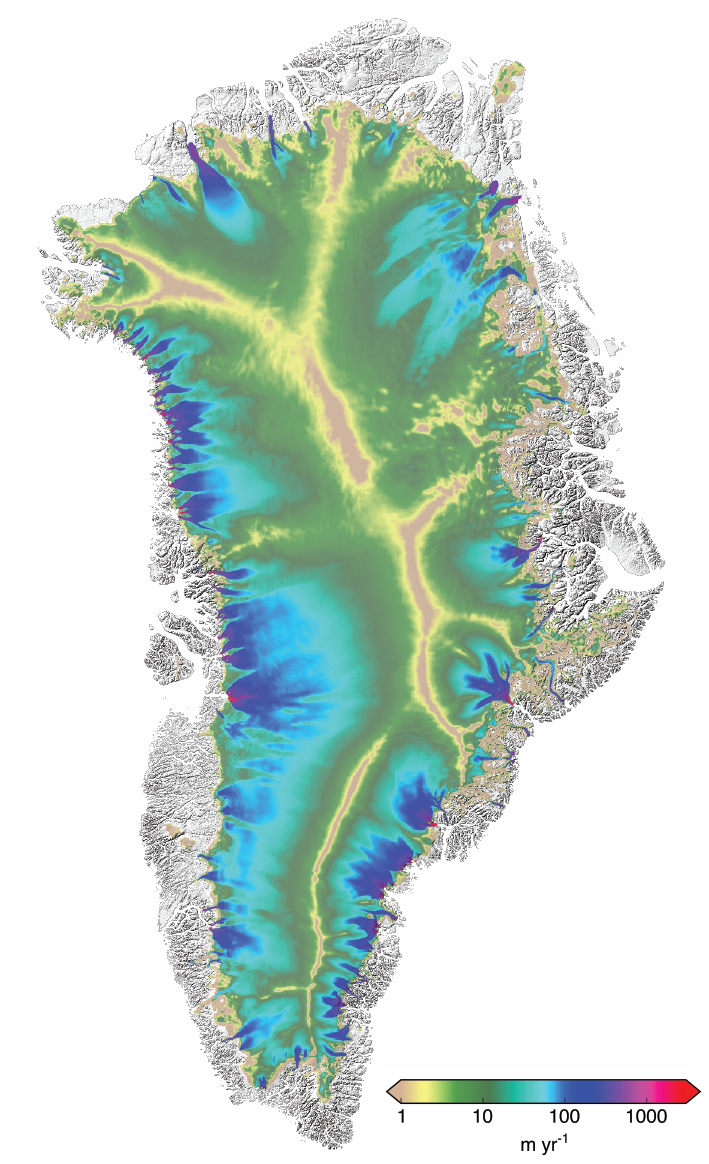
\includegraphics[width=3.0in,keepaspectratio=true]{gris-flow-600m}

    \vfill

    \small Support by email: \PISMEMAIL.
    \medskip

    Manual date \today. Based on PISM \PISMREV.
    \medskip

    \PISMDOWNLOADMSG
  \end{center}
\end{titlepage}

\newpage
\phantom{bob}

\centerline{\textsc{Authorship}}
\bigskip

\normalspacing
PISM is a joint project between developers in the ice sheet modeling group at the University of Alaska (UAF), developers at the Potsdam Institute for Climate Impact Research (PIK), and several additional developers listed here.  Current (or recent) affiliation and area of contributions shown:
\bigskip
\normalspacing

\renewcommand{\arraystretch}{1.3}
\begin{tabular}{ll}
\textbf{Torsten Albrecht (PIK)} & ice shelf physics and numerics \\
\textbf{\underline{Andy Aschwanden} (UAF)} & \begin{minipage}[t]{4in} scripts, visualization, thermodynamics, SeaRISE-Greenland  \end{minipage}  \\
\textbf{Jed Brown (ANL)} & source code original author, SSA numerics, PETSc underpinnings \\
\textbf{\underline{Ed Bueler} (UAF)} & \begin{minipage}[t]{4in} principal investigator, verification, earth deformation, SIA numerics, thermodynamics, documentation  \end{minipage} \\
\textbf{Dani DellaGiustina (UAF)} & regional tools and modeling \\
\textbf{Johannes Feldman (PIK)} & marine ice sheet processes \\
\textbf{Bob Fischer (GFDL)} & coupling design \\
\textbf{Marijke Habermann (UAF)} & inversion\\
\textbf{Marianne Haseloff (UBC)} & ice streams: physics and numerics\\
\textbf{Regine Hock (UAF)} & surface mass and energy balance \\
\textbf{\underline{Constantine Khroulev} (UAF)} & \begin{minipage}[t]{4in} source code primary author, input/output, software design, climate couplers, parallelization, testing, user support, most documentation, most bug fixes, regional tools, \dots \end{minipage} \\
\textbf{Anders Levermann (PIK)} & calving, ice shelf processes \\
\textbf{Craig Lingle (UAF)} & original SIA model, earth deformation \\
\textbf{Maria Martin (PIK)} & SeaRISE-Antarctica, Antarctica processes \\
\textbf{Mattias Mengel (PIK)} & marine ice sheet processes \\
\textbf{David Maxwell (UAF)} & inversion, SSA finite elements, python bindings \\
\textbf{Ward van Pelt (IMAU)} & hydrology analysis and design \\
\textbf{Julien Seguinot (INK)} & bug fixes, temperature index model \\
\textbf{Ricarda Winkelmann (PIK)} & Antarctica processes, coupling, and modeling  \\
\textbf{Florian Ziemen (UAF)} & bug fixes, sliding \\
\end{tabular}

\bigskip
\noindent Email the \underline{underlined} UAF developers at \qquad \PISMEMAIL.

\bigskip\bigskip
\noindent \textsc{Front page}:  Magnitude of horizontal surface velocity from PISM run on a horizontal grid resolution of 600\,m.  Visualization by QGIS.

\vfill

\newpage
\vspace{0.2in}
\begin{quote}
\textsl{Copyright (C) 2004--2014 The PISM Authors}
\medskip

\noindent \textsl{This file is part of PISM.  PISM is free software; you can redistribute it and/or modify it under the terms of the GNU General Public License as published by the Free Software Foundation; either version 3 of the License, or (at your option) any later version.  PISM is distributed in the hope that it will be useful, but WITHOUT ANY WARRANTY; without even the implied warranty of MERCHANTABILITY or FITNESS FOR A PARTICULAR PURPOSE.  See the GNU General Public License for more details.  You should have received a copy of the GNU General Public License\index{GPL (\emph{GNU Public License})} along with PISM; see \emph{\texttt{COPYING}}.  If not, write to the Free Software Foundation, Inc., 51 Franklin St, Fifth Floor, Boston, MA  02110-1301 USA}
\end{quote}
\vspace{0.5in}

\centerline{\textsc{Acknowledgements}}
\bigskip

\small
NASA Modeling, Analysis, and Prediction (MAP) program\index{Organizations!NASA!Modeling, Analysis, and Prediction program} grant \# NNX13AM16G and NASA Cryospheric Sciences program grant \# NNX13AK27G support the development of PISM from 2013 to 2017.  NASA MAP grant \# NNX09AJ38G supported the development of PISM from 2009 to 2013.  Development from 2002 to 2008 was supported by the NASA Cryospheric Sciences program\index{Organizations!NASA!Cryospheric Sciences program}.

The Snow, Ice, and Permafrost group\index{Organizations!Geophysical Institute!Snow, Ice, and Permafrost group} at the Geophysical Institute is the home for the University of Alaska PISM developers; find us in Elvey 410D.  The Arctic Region Supercomputing Center\index{Organizations!Arctic Region Supercomputing Center (ARSC)} has provided significant computational resources and technical help in the development of PISM.

Thanks for comments/questions from many PISM users around the world, including these not already listed as PISM authors:

\begin{quote}
Tolly A{\dh}algeirsd{\'o}ttir, Antje Fitzner, Nick Golledge, Tore Hattermann, Moritz H\"utten, Thomas Kleiner, Leo van Kampenhout, Marianne Madsen, Malou Maris, Tim Morey, Mirena Olaizola, Christian Rodehacke, Nathan Shemonski, Sebastian Simonsen, Anne Solgaard, Ben Sperisen, Synne H\o{}yer Svendsen, Martin Truffer, Shuting Yang, Ryan Woodard
\end{quote}

\noindent for helpful comments and questions on PISM and this \emph{Manual}.  Dave Covey, Don Bahls, and Greg Newby have supported our hardware, software, and computations.  Bob Bindschadler, Sophie Nowicki, Jesse Johnson, and others in the SeaRISE\index{SeaRISE!group} group have motivated and assisted PISM development in many ways.

\normalsize



\newpage
\setcounter{tocdepth}{3}
\small
\tableofcontents
\normalsize

\newpage


\section{Introduction}\label{sec:intro}

Welcome!  All information about PISM is online at the home page
\begin{center}
  \url{http://www.pism-docs.org}
\end{center}
Please see the extensive lists of PISM publications and applications at that page.

This User's Manual gives examples of how to run PISM using publicly-available data for: the whole Greenland ice sheet, the Jakobshavn outlet glacier in Greenland, the Ross ice shelf in Antarctica, and a number of simplified geometry tests.  It documents all the PISM options.  It summarizes the continuum models used by PISM, and it illustrates how PISM's numerical approximations are verified.

See the PISM Installation Manual\footnote{PDF for latest stable release at \url{https://github.com/pism/pism/blob/dev/INSTALL.md}.}
for how to download\index{PISM!download source code} the PISM source code and install
it\index{PISM!install}, along with needed libraries.  The PISM Climate Forcing
Manual\footnote{PDF for latest stable release at \url{http://www.pism-docs.org/wiki/lib/exe/fetch.php?media=pism_forcing.pdf}.}
extends the User's Manual to cover additional couplings to atmosphere and ocean
models and data.

Users who want to understand more deeply how PISM is designed, or who want to extend it,  will need to go beyond what is described here.  See the \emph{Source Code Browser}\index{PISM!\emph{Source Code Browser (HTML)}}, which is online for the latest stable version.\footnote{At \url{http://www.pism-docs.org/wiki/doku.php?id=browser}.}  It can be generated from source code as described in the PISM Installation Manual.  It gives a complete view of the class/object structure of the PISM source code.


\vspace{.3in}
  
\begin{center}
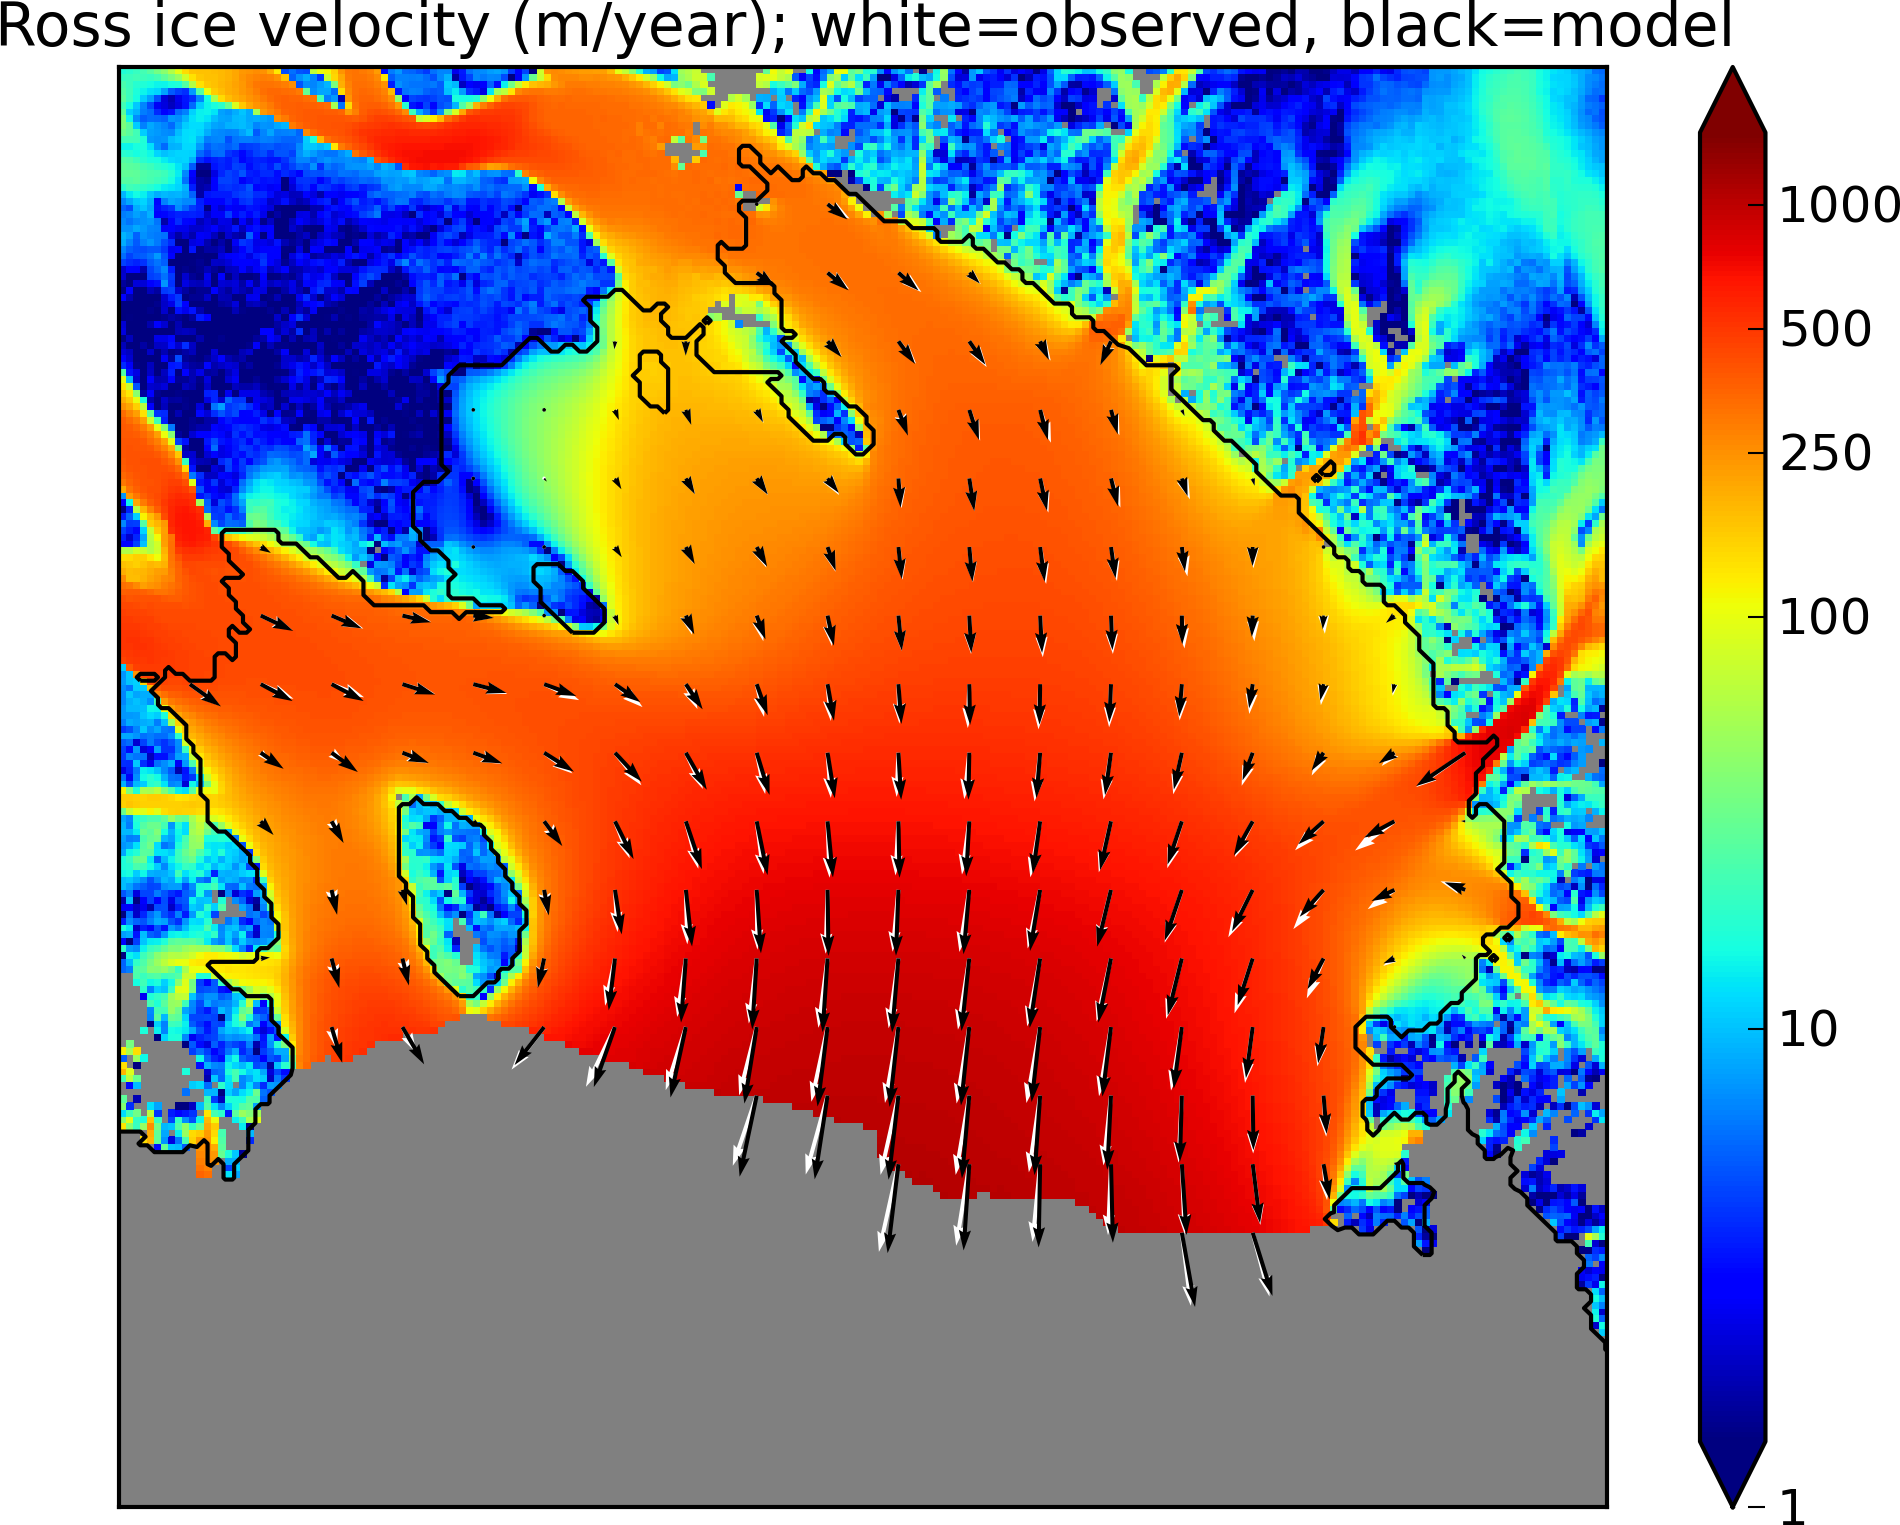
\includegraphics[width=3.5in,keepaspectratio=true]{rossquiver}
\end{center}

\vspace{.2in}

\begin{center}
\framebox{\parbox{5.0in}{ \emph{WARNING}:\index{PISM!warning}  PISM is an ongoing research project.  Ice sheet modeling requires many choices.  Please don't trust the results of PISM or any other ice sheet model without a fair amount of exploration.  Also, please don't expect all your questions to be answered here.  Write to us with questions at \PISMEMAIL.} }
\end{center}


\clearpage\newpage
\section{Getting started}\label{sec:start}\index{PISM!getting started}

This introduction is intended to be interactive and participatory, and it should work on \emph{your personal machine} as well as on a supercomputer.  Please try the commands and view the resulting files.  Do the runs with your own values for the options.  We can't hide the fact that PISM has lots of ``control knobs,'' but fiddling with them will help you get going.  Give it a try!

To install PISM see the \emph{Getting PISM} tab at \href{http://www.pism-docs.org}{\texttt{www.pism-docs.org}}.  Or get the PISM Installation Manual (PDF) at \url{http://www.pism-docs.org/wiki/lib/exe/fetch.php?media=installation.pdf}.  Once PISM is installed, the executable \texttt{pismr} should be available on your system's ``path''; confirm this with ``\texttt{which pismr}''.  The instructions below assume you are using a \texttt{bash} shell or one that accepts \texttt{bash} syntax.  They also assume you have the PISM source code in the directory ``\texttt{pism/}''.

\subsection{A Greenland ice sheet example}

We get started with an extended example showing how to generate initial states for prognostic model experiments on the Greenland ice sheet.  Ice sheet and glacier model studies often involve modeling present and past states using actions like the ones demonstrated here.  Our particular choices made here are motivated by the evaluation of initialization methods in \cite{AschwandenAdalgeirsdottirKhroulev}.

We use data assembled by the \href{http://websrv.cs.umt.edu/isis/index.php/SeaRISE_Assessment}{Sea-level Response to Ice Sheet Evolution (SeaRISE)} assessment process\index{SeaRISE!data} \cite{Bindschadler2013SeaRISE}.  SeaRISE is a community-organized assessment process providing an upper bound on ice sheet contributions to sea level in the next 100--200 years, especially for the IPCC AR5 report in 2013.

This example is a hands-on first look at PISM.  It is not an in-depth tutorial, and some details of what is happening are only explained later in this Manual, which thoroughly discusses PISM options, nontrivial modeling choices, and how to preprocess input data.

The basic runs here, mostly on coarse $20$ and $10\,\textrm{km}$ grids, can be done on a typical workstation or laptop.  PISM is, however, designed to make high resolution (e.g.~$5\,\textrm{km}$ to $1\,\textrm{km}$ grids for whole-Greenland ice sheet modeling) possible by exploiting large-scale parallel processing.  See \cite{AschwandenAdalgeirsdottirKhroulev,Golledgeetal2012,Golledgeetal2013}, among other published high-resolution PISM examples.


\subsection{Input data}

The NetCDF data used to initialize SeaRISE runs is freely-available online: 
\medskip

\centerline{\protect{\textbf{\url{http://websrv.cs.umt.edu/isis/index.php/Present_Day_Greenland}}}}
\medskip

\noindent To download the specific file we want, namely \texttt{Greenland_5km_v1.1.nc}, and preprocess it for PISM, do:
\begin{verbatim}
$ cd pism/examples/std-greenland
$ ./preprocess.sh
\end{verbatim}
\noindent The script \texttt{preprocess.sh} requires \texttt{wget} and also the NetCDF Operators (``NCO''; \url{http://nco.sourceforge.net/}).  It downloads the version 1.1 of the SeaRISE ``master'' present-day data set, which contains ice thickness and bedrock topography from BEDMAP \cite{BamberLayberryGogenini}, and modeled precipitation and surface mass balance rates from RACMO \cite{Ettemaetal2009}, among other fields.

In particular, it creates three new NetCDF files which can be read by PISM.  The spatially-varying fields, with adjusted metadata, go in \texttt{pism_Greenland_5km_v1.1.nc}.  The other two new files contain famous time-dependent paleo-climate records from ice and seabed cores: \texttt{pism_dT.nc} has the GRIP temperature record \cite{JohnsenetalGRIP} and \texttt{pism_dSL.nc} has the SPECMAP sea level record \cite{Imbrieetal1984}.

Any of these NetCDF files can be viewed with \texttt{ncview} or other NetCDF visualization tools; see Table \ref{tab:NetCDFview} below.  An application of IDV to the master data set produced Figure \ref{fig:sr-input}, for example.  Use \texttt{ncdump -h} to see the metadata and history of the files.

\begin{figure}[ht]
\centering
\mbox{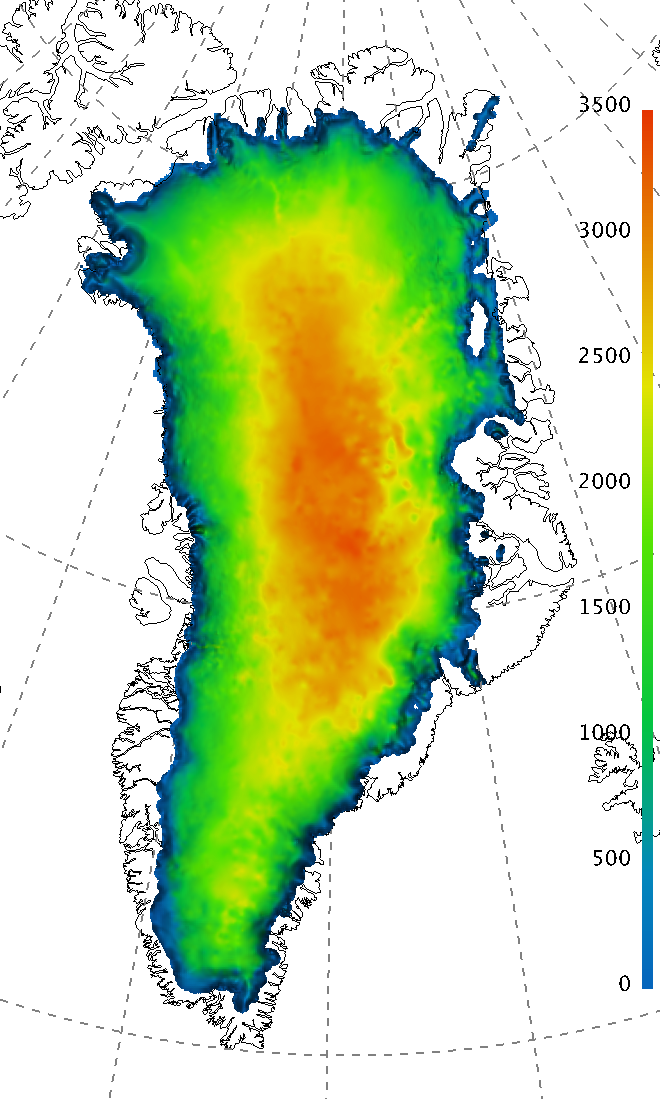
\includegraphics[width=2.0in,keepaspectratio=true]{sr-greenland-thk}
  \qquad
  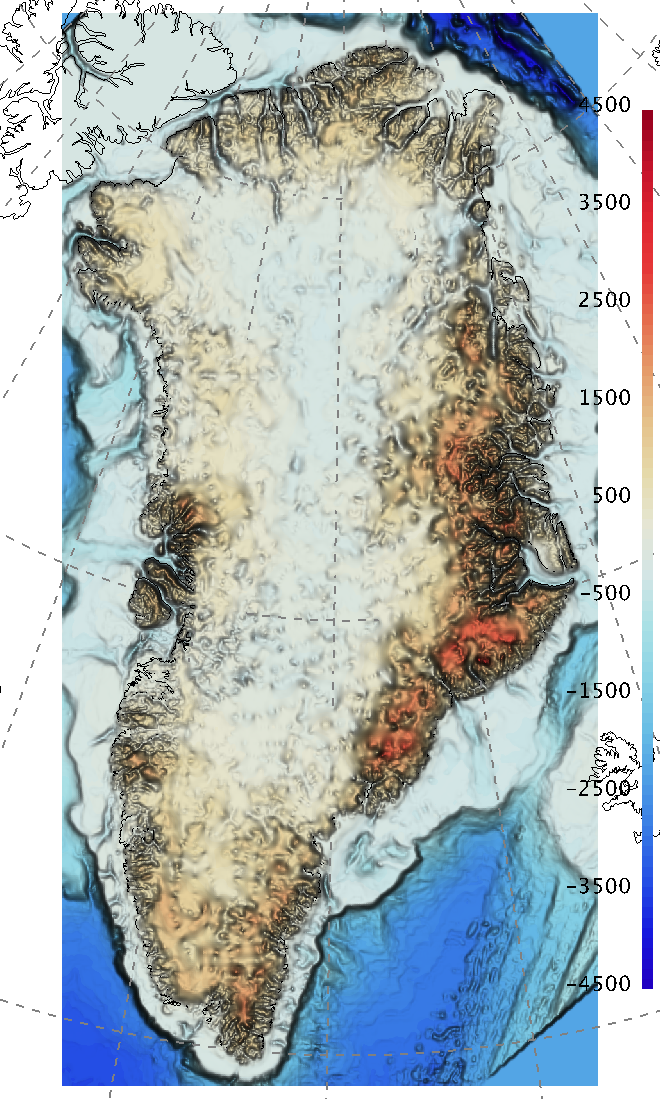
\includegraphics[width=2.0in,keepaspectratio=true]{sr-greenland-topg}
  \qquad
  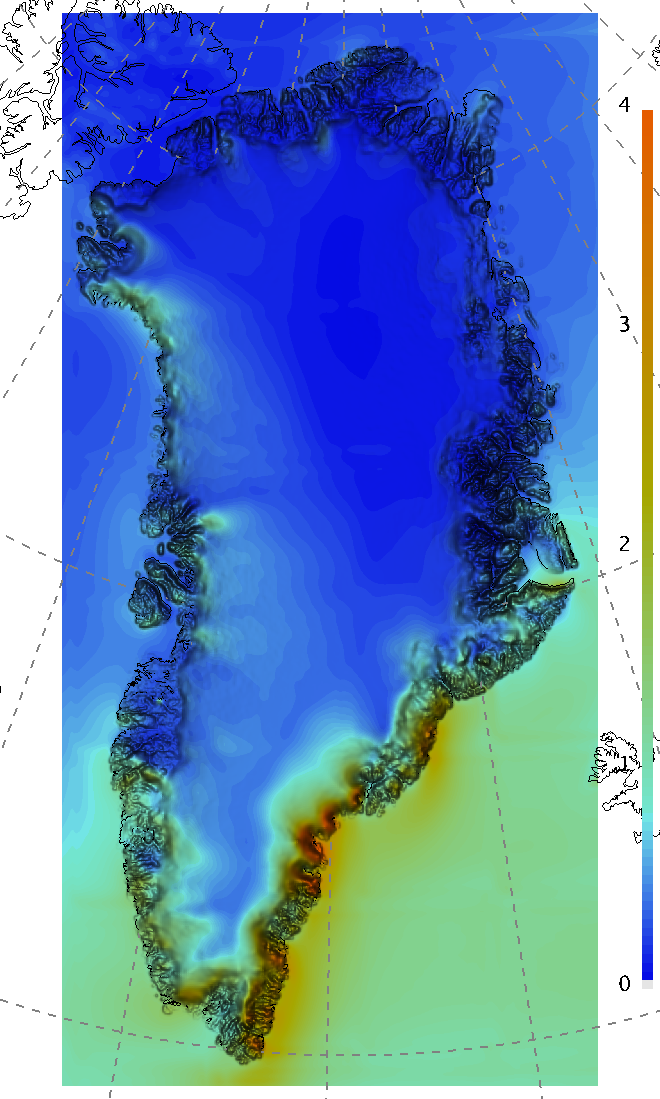
\includegraphics[width=2.0in,keepaspectratio=true]{sr-greenland-prcp}}
\caption{The input file contains present-day ice thickness (left; m), bedrock elevation (center; m), and present-day precipitation (right; m $\text{a}^{-1}$ ice equivalent) for SeaRISE-Greenland.  These are fields \texttt{thk}, \texttt{topg}, and \texttt{precipitation}, respectively, in \texttt{pism_Greenland_5km_v1.1.nc}.}
\label{fig:sr-input}
\end{figure}


\subsection{First run}   \label{subsect:runscript}  Like many Unix programs, PISM allows a lot of command-line options.  In fact, because the variety of allowed ice sheet, shelf, and glacier configurations, and included sub-models, is so large, the list of possible command-line options covers sections \ref{sec:initboot} through \ref{sec:practical-usage} of this manual.  In practice one often builds scripts to run PISM with the correct options, which is what we show here.  The script we use is ``\texttt{spinup.sh}'' in the \texttt{examples/std-greenland/} subdirectory of \texttt{pism/}.

Note that initializing ice sheets, generically called ``spin-up'', can be done by computing approximate steady states with constant boundary data, or, in some cases, by integrating paleo-climatic and long-time-scale information, also applied at the ice sheet boundary, to build a model for the present state of the ice sheet.  Both of these possibilities are illustrated in the \texttt{spinup.sh} script.  The spin-up stage of using an ice sheet model may actually require more processor-hours than follow-on ``experiment'' or ``forecast'' stages.

To see what can be done with the script, read the usage message it produces:
\begin{verbatim}
$ ./spinup.sh
\end{verbatim}

The simplest spin-up approach is to use a ``constant-climate'' model.  We take this approach first.  To see a more detailed view of the PISM command for the first run, do:
\begin{verbatim}
$ PISM_DO=echo ./spinup.sh 4 const 10000 20 sia g20km_10ka.nc
\end{verbatim}
Setting the environment variable \texttt{PISM_DO} in this way tells \texttt{spinup.sh} just to print out the commands it is about to run, not do them.  The ``proposed'' run looks like this:
\label{firstcommand}
\small
\begin{verbatim}
mpiexec -n 4 pismr -boot_file pism_Greenland_5km_v1.1.nc -Mx 76 -My 141 \
  -Mz 101 -Mbz 11 -z_spacing equal -Lz 4000 -Lbz 2000 -skip -skip_max 10 \
  -ys -10000 -ye 0 -surface given -surface_given_file pism_Greenland_5km_v1.1.nc \
  -calving ocean_kill pism_Greenland_5km_v1.1.nc -sia_e 3.0 \
  -ts_file ts_g20km_10ka.nc -ts_times -10000:yearly:0 \
  -extra_file ex_g20km_10ka.nc -extra_times -10000:100:0 \
  -extra_vars diffusivity,temppabase,tempicethk_basal,bmelt,tillwat,csurf,mask,thk,topg,usurf \
  -o g20km_10ka.nc
\end{verbatim}
\normalsize
Let's briefly deconstruct this run.

At the front is ``\texttt{mpiexec -n 4 pismr}''.  This means that the PISM executable \texttt{pismr} is run in parallel on four processes parallel standard (e.g.~cores) under the Message Passing Interface (``MPI''; \url{http://www.mcs.anl.gov/mpi/}).  Though we are assuming you have a workstation or laptop with at least 4 cores, this example will work with 1 to about 50 processors, with reasonably good scaling in speed.  Scaling can be good with more processors if we run at higher spatial resolution \cite{BBssasliding,DickensMorey2013}.  The executable name ``\texttt{pismr}'' stands for the standard ``run'' mode of PISM (in contrast to specialized modes described later in sections \ref{sec:verif} and \ref{sec:simp}).

Next, the proposed run uses option \texttt{-boot_file} to start the run by ``bootstrapping.'' This term describes the creation, by heuristics and highly-simplified models, of the mathematical initial conditions required for a deterministic, time-dependent ice dynamics model.  Then the options describe a $76\times 141$ point grid in the horizontal, which gives 20 km grid spacing in both directions.  Then there are choices about the vertical extent and resolution of the computational grid; more on those later.  After that we see a description of the time-axis, with a start and end time given: ``\texttt{-ys -10000 -ye 0}''.

Then we get the instructions that tell PISM to read the upper surface boundary conditions (i.e.~climate) from a file: ``\texttt{-surface given -surface_given_file pism_Greenland_5km_v1.1.nc}''.  For more on these choices, see subsection \ref{sec:climate-inputs}, and also the PISM Climate Forcing Manual.

Then there are a couple of options related to ice dynamics.  First is a minimal calving model which removes ice at the calving front location given by a thickness field in the input file (``\texttt{-calving ocean_kill}''); see subsection \ref{sec:calving} for this and other calving options).  Then there is a setting for enhanced ice softness (``\texttt{-sia_e 3.0}'').  See subsection \ref{sec:rheology} for more on this enhancement parameter, which we also return to later in the current section in a parameter study.

Then there are longish options describing the fields we want as output, including scalar time series (``\texttt{-ts_file ts_g20km_10ka.nc -ts_times -10000:yearly:0}''; see section \ref{sec:practical-usage}) and space-dependent fields (``\texttt{-extra_file ...}''; again see section \ref{sec:practical-usage}), and finally the named output file (``\texttt{-o g20km_10ka.nc}'').

Note that the modeling choices here are reasonable, but they are not the only way to do it! The user is encouraged to experiment; that is the point of a model.

Now let's actually get the run going:
\begin{verbatim}
$ ./spinup.sh 4 const 10000 20 sia g20km_10ka.nc &> out.g20km_10ka &
\end{verbatim}
\noindent The terminating ``\verb|&|'' asks unix to run the command in the background, so we can keep working in the current shell.  Because we have re-directed the text output (``\verb|&> out.g20km_10ka|''), PISM will show what it is doing in the text file \texttt{out.g20km_10ka}.  Using \texttt{less} is a good way to watch such a growing text-output file.  This run should take only 20 minutes or so.


\subsection{Watching the first run}  \label{subsect:watchrun}  As soon as the run starts it creates time-dependent NetCDF files \texttt{ts_g20km_10ka.nc} and \texttt{ex_g20km_10ka.nc}.  The latter file, which has spatially-dependent fields at each time, is created after the first 100 model years, a few wall clock seconds in this case.  The command \texttt{-extra_file ex_g20km_10ka.nc -extra_times -10000:100:0} adds a spatially-dependent ``frame'' at model times -9900, -9800, \dots, 0.

To look at the spatial-fields output graphically, do:
\begin{verbatim}
$ ncview ex_g20km_10ka.nc
\end{verbatim}
We see that \texttt{ex_g20km_10ka.nc} contains growing ``movies'' of the fields chosen by the \texttt{-extra_vars} option.  A frame of the ice thickness field \texttt{thk} is shown in Figure \ref{fig:growing} (left).

The time-series file \texttt{ts_g20km_10ka.nc} is also growing.  It contains spatially-averaged ``scalar'' diagnostics like the total ice volume or the ice-sheet-wide maximum velocity (variable \texttt{ivol} and \texttt{max_hor_vel}, respectively).  It can be viewed
\begin{verbatim}
$ ncview ts_g20km_10ka.nc
\end{verbatim}
The growing time series for \texttt{ivol} is shown in Figure \ref{fig:growing} (right).  Recall that our intention was to generate a minimal model of the Greenland ice sheet in approximate steady-state with a steady (constant-in-time) climate.  The measurable steadiness of the \texttt{ivol} time series is a possible standard for steady state \cite[for example]{EISMINT00}.

\begin{figure}[ht]
\centering
\mbox{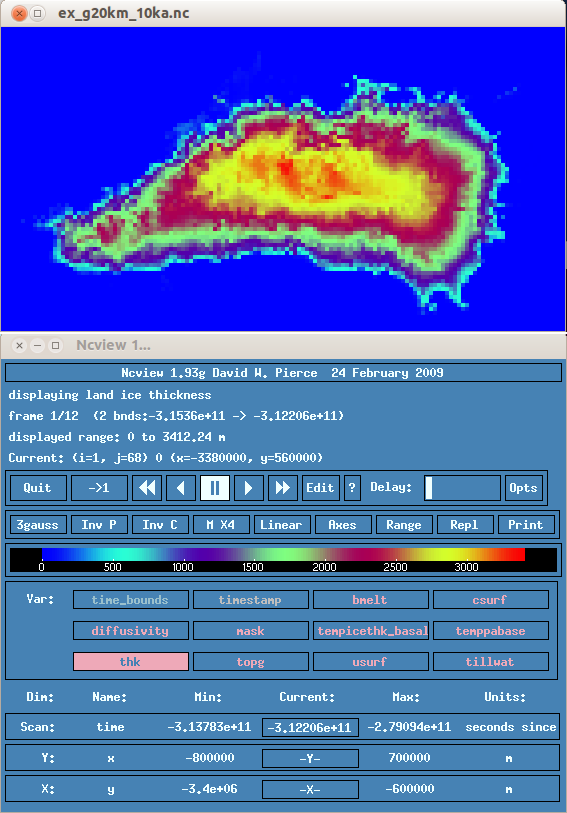
\includegraphics[height=5.0in,keepaspectratio=true]{ex-growing-thk-g20km}
  \qquad 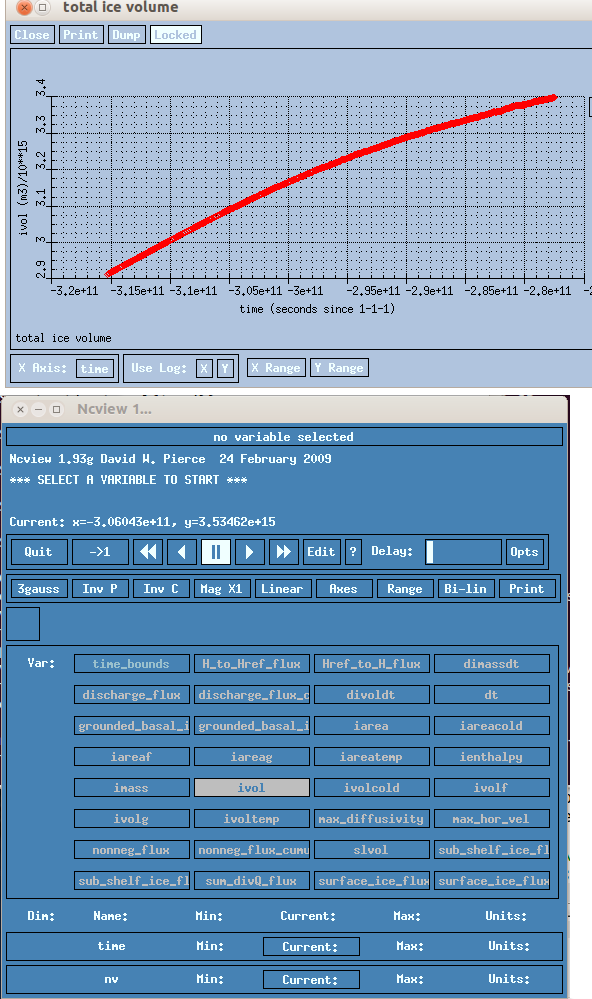
\includegraphics[height=5.0in,keepaspectratio=true]{ts-growing-ivol-g20km}}
\caption{Two views produced by \texttt{ncview} during a PISM model run.  Left: \texttt{thk}, the ice sheet thickness, a space-dependent field, from file \texttt{ex_g20km_10ka.nc}.  Right: \texttt{ivol}, the total ice sheet volume time-series, from file \texttt{ts_g20km_10ka.nc}.}
\label{fig:growing}
\end{figure}

At the end of the run the output file \texttt{g20km_10ka.nc} is generated.  Figure \ref{fig:firstoutput} shows some fields from this file.  In the next subsections we consider their ``quality'' as model results.  To see a report on computational performance, we do:
\begin{verbatim}
$ ncdump -h g20km_10ka.nc |grep history
    :history = "user@machine 2013-11-23 15:57:22 AKST: PISM done.  Performance stats:
0.3435 wall clock hours, 1.3738 proc.-hours, 7274.0065 model years per proc.-hour,
PETSc MFlops = 0.03.\n",
\end{verbatim}

\begin{figure}[ht]
\centering
\mbox{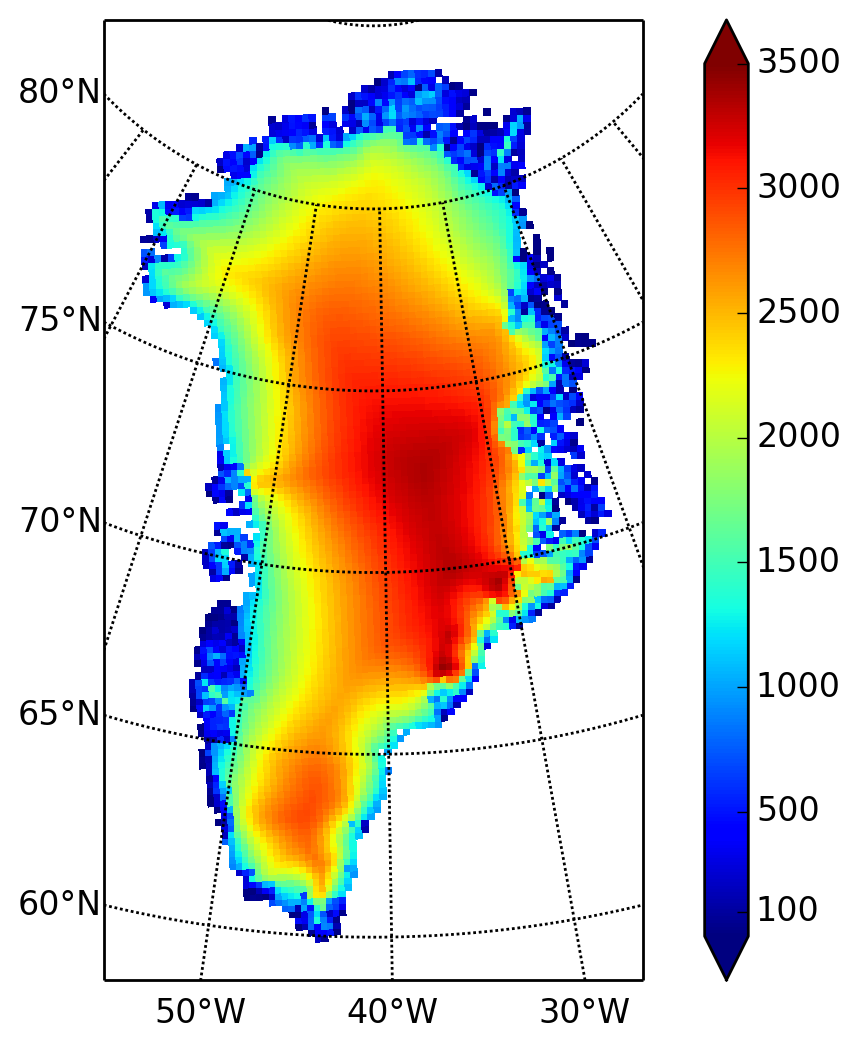
\includegraphics[height=2.75in,keepaspectratio=true]{g20km-10ka-usurf} 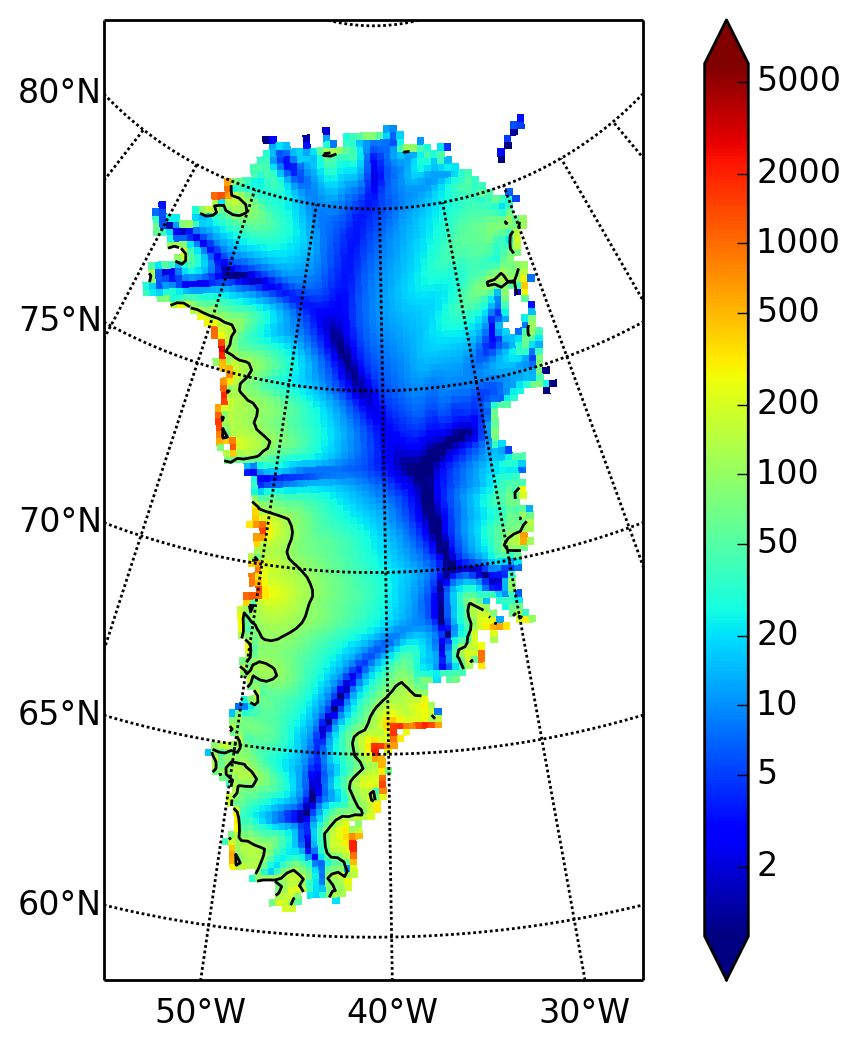
\includegraphics[height=2.75in,keepaspectratio=true]{g20km-10ka-csurf} 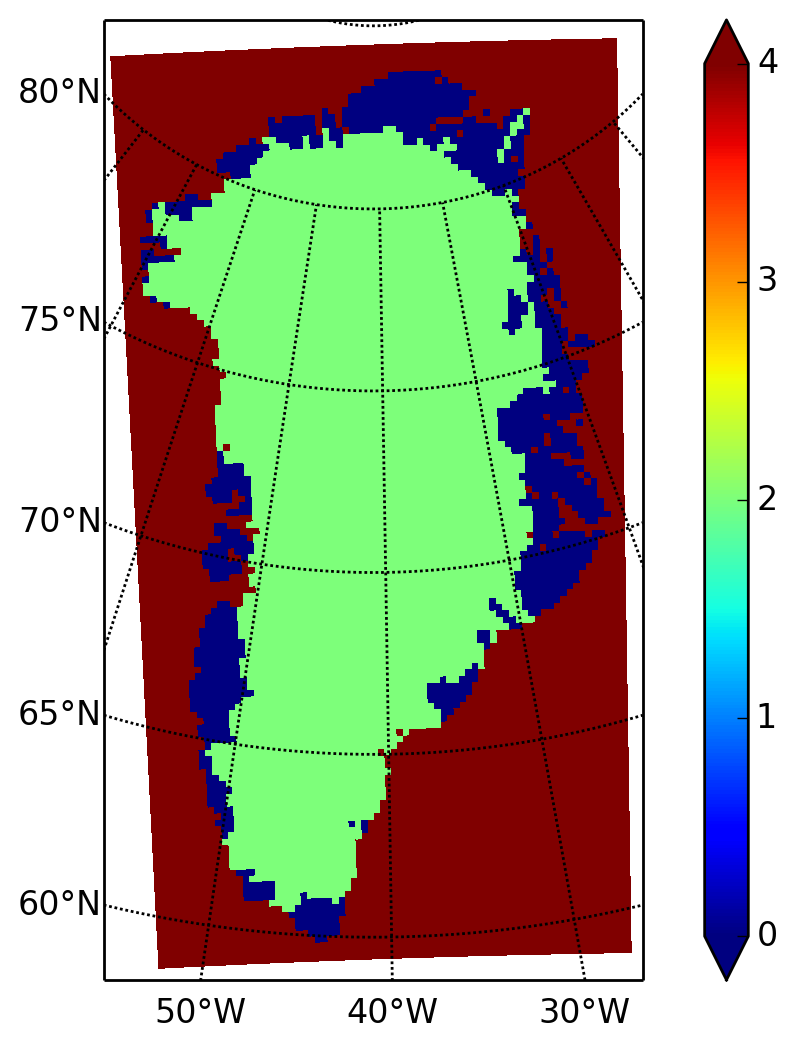
\includegraphics[height=2.75in,keepaspectratio=true]{g20km-10ka-mask}}
\caption{Fields from output file \texttt{g20km_10ka.nc}.  Left: \texttt{usurf}, the ice sheet surface elevation in meters.  Middle: \texttt{csurf}, the surface speed in meters/year ($=$ m/a), including the 100 m/a contour (solid black).  Right: \texttt{mask}, with 0 = ice-free land, 2 = grounded ice, 4 = ice-free ocean.}
\label{fig:firstoutput}
\end{figure}


\subsection{Second run: a better ice-dynamics model}  \label{subsect:ssarun}

It is widely-understood that ice sheets slide on their bases, especially when liquid water is present at the base (see \cite{Joughinetal2001,MacAyeal}, among others).  An important aspect of modeling such sliding is the inclusion of membrane or ``longitudinal'' stresses into the stress balance \cite{BBssasliding}.  The basic stress balance in PISM which involves membrane stresses is the Shallow Shelf Approximation (SSA) \cite{WeisGreveHutter}.  The stress balance used in the previous section was, by contrast, the (thermomechanically-coupled) non-sliding, non-membrane-stress Shallow Ice Approximation (SIA) \cite{BBL,EISMINT00}.  The preferred ice dynamics model within PISM, that allows both sliding balanced by membrane stresses and shear flow as described by the SIA, is the SIA+SSA ``hybrid'' model \cite{BBssasliding,Winkelmannetal2011}.  For more on stress balance theories see section \ref{sec:dynamics} of this Manual.

The practical issue with models of sliding is that a distinctly-uncertain parameter space must be introduced.  This especially involves parameters controlling the amount and pressure of subglacial water (see \cite{AschwandenAdalgeirsdottirKhroulev,Clarke05,Tulaczyketal2000,vanPeltOerlemans2012} among other references).  In this regard, PISM uses the concept of a saturated and pressurized subglacial till with a modeled distribution of yield stress  \cite{BBssasliding,SchoofStream}.  The yield stress arises from the PISM model of the production of subglacial water, which is itself computed through the conservation of energy model \cite{AschwandenBuelerKhroulevBlatter}.  We use such models in the rest of this Getting Started section.

While the \texttt{spinup.sh} script has default sliding-related parameters, for demonstration purposes we change one parameter.  We replace the default power $q=0.25$ in the sliding law (the equation which relates both the subglacial sliding velocity and the till yield stress to the basal shear stress which appears in the SSA stress balance) by a less ``plastic'' and more ``linear'' choice $q=0.5$.  See subsection \ref{subsect:basestrength} for more on sliding laws.  To see the run we propose, do
\begin{verbatim}
$ PISM_DO=echo PARAM_PPQ=0.5 ./spinup.sh 4 const 10000 20 hybrid g20km_10ka_hy.nc
\end{verbatim}
Now remove ``\texttt{PISM_DO=echo}'' and redirect the text output into a file to start the run:
\begin{verbatim}
$ PARAM_PPQ=0.5 ./spinup.sh 4 const 10000 20 hybrid g20km_10ka_hy.nc &> out.g20km_10ka_hy &
\end{verbatim}
This run might take 30 minutes or so.\footnote{Regarding the relative speeds of the runs that produce \texttt{g20km_10ka.nc} and \texttt{g20km_10ka_hy.nc}, note that the computation of the SSA stress balance is substantially more expensive than the SIA in a per-step sense.  However, the SSA stress balance in combination with the mass continuity equation causes the maximum diffusivity in the ice sheet to be substantially lower during the run.  Because the maximum diffusivity controls the time-step in the PISM adaptive time-stepping scheme \cite{BBL}, the number of time steps is reduced in the hybrid run.  To see this contrast do\, \texttt{ncview ts_g20km_10ka*nc}\, and view variables \texttt{max_diffusivity} and \texttt{dt}. }

When this run is finished it produces \texttt{g20km_10ka_hy.nc}.  As before do
\begin{verbatim}
$ ncdump -h g20km_10ka_hy.nc |grep history
\end{verbatim}
to see performance results for your machine.  The number reported as ``\texttt{PETSc MFlops}'' from this run is about $2.6 \times 10^5$, much larger than the previous run, because now calls to the PETSc library are used when solving the non-linear and non-local SSA stress balance in parallel.

The results of this run are shown in Figure \ref{fig:secondoutputcoarse}.  We show the basal sliding speed field \texttt{cbase} in this Figure, where Figure \ref{fig:firstoutput} had the \texttt{mask}, but the reader can check that \texttt{cbase}=0 in the nonsliding SIA-only result \texttt{g20km_10ka.nc}.

\begin{figure}[ht]
\centering
\mbox{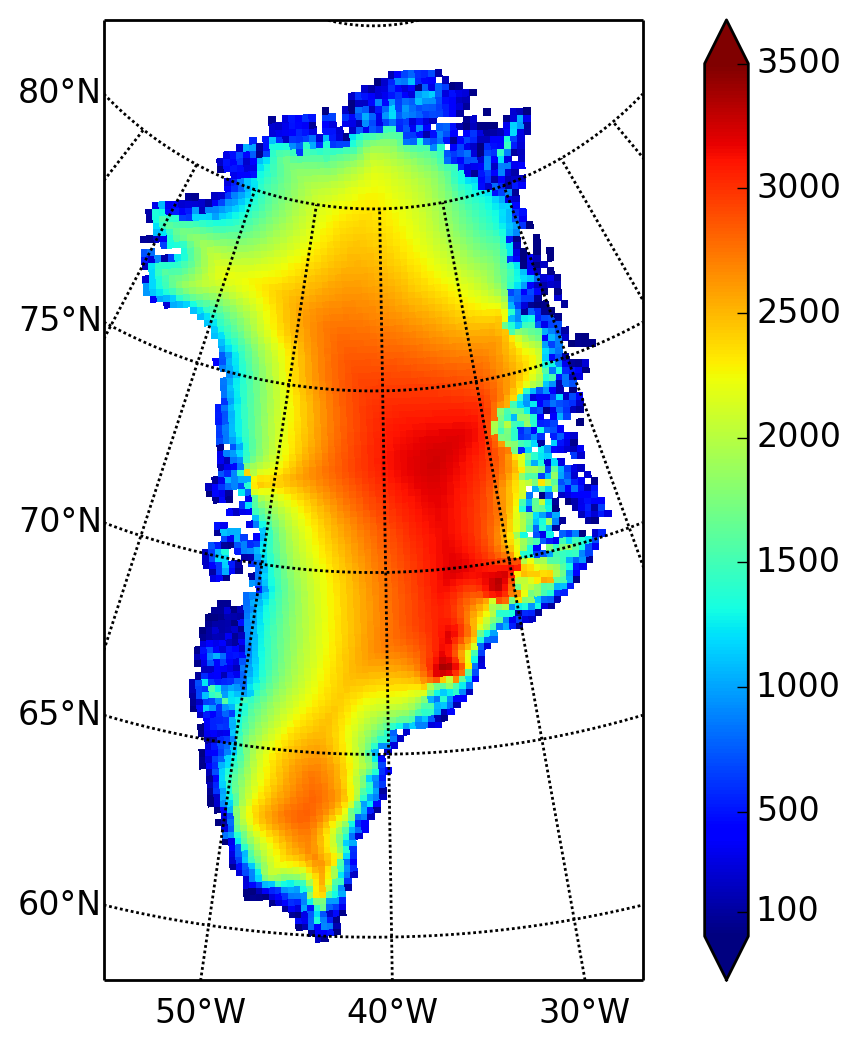
\includegraphics[height=2.75in,keepaspectratio=true]{g20km-10ka-hy-usurf} 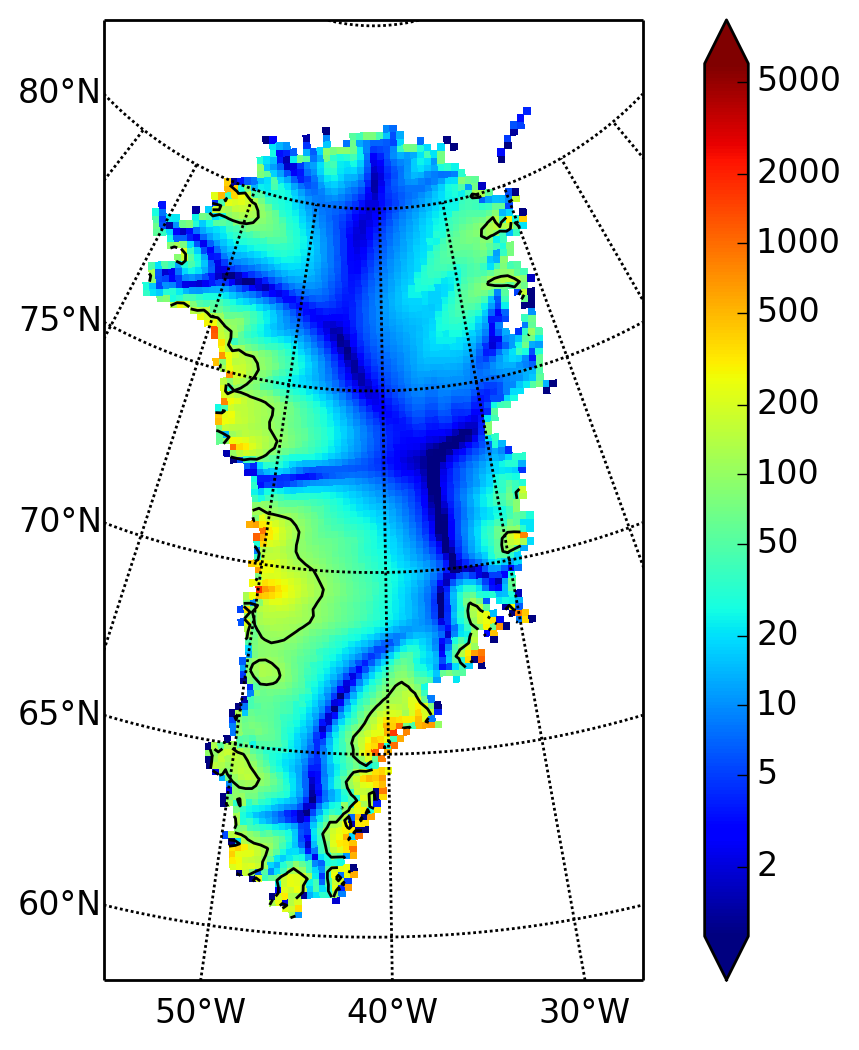
\includegraphics[height=2.75in,keepaspectratio=true]{g20km-10ka-hy-csurf} 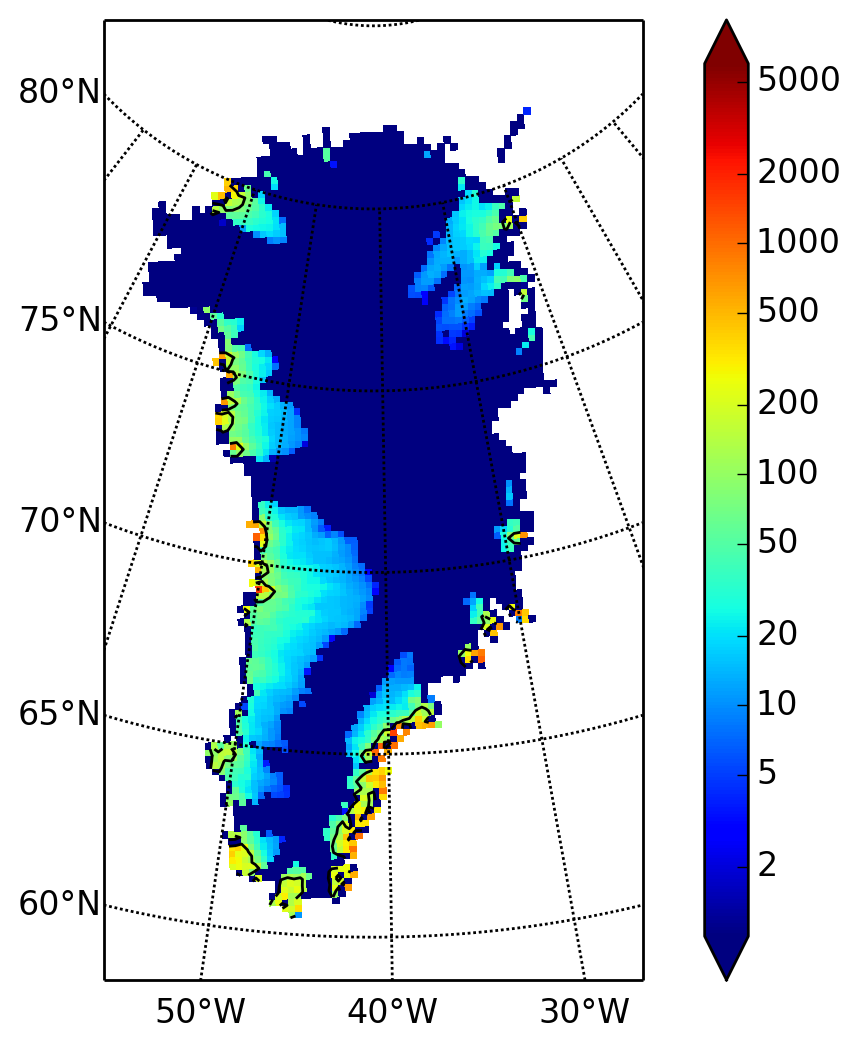
\includegraphics[height=2.75in,keepaspectratio=true]{g20km-10ka-hy-cbase}}
\caption{Fields from output file \texttt{g20km_10ka_hy.nc}.  Left: \texttt{usurf}, the ice sheet surface elevation in meters.  Middle: \texttt{csurf}, the surface speed in m/a, including the 100 m/a contour (solid black).  Right: the sliding speed \texttt{cbase}, shown the same way as \texttt{csurf}.}
\label{fig:secondoutputcoarse}
\end{figure}

The hybrid model includes sliding, and it is important to evaluate that aspect of the output.  However, though it is critical to the response of the ice to changes in climate, basal sliding velocity is essentially unobservable in real ice sheets.  On the other hand, because of relatively-recent advances in radar and image technology and processing \cite{Joughin2002}, the surface velocity of an ice sheet is an observable.  So, how good is our model result for this quantity, namely \texttt{csurf}?  Figure \ref{fig:csurfvsobserved} compares the radar-observed \texttt{surfvelmag} field in the downloaded SeaRISE-Greenland data file \texttt{Greenland_5km_v1.1.nc} with the just-computed PISM result.

\begin{figure}[ht]
\centering
\mbox{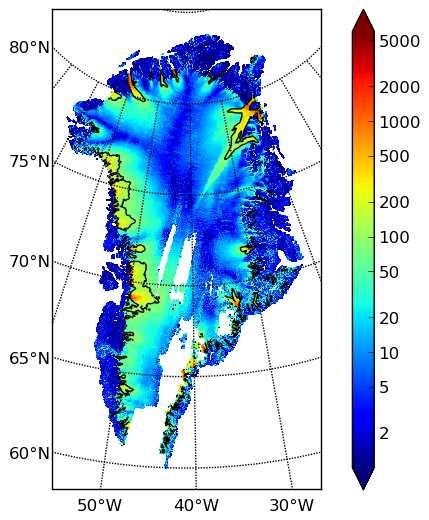
\includegraphics[height=2.75in,keepaspectratio=true]{Greenland-5km-v1p1-surfvelmag} 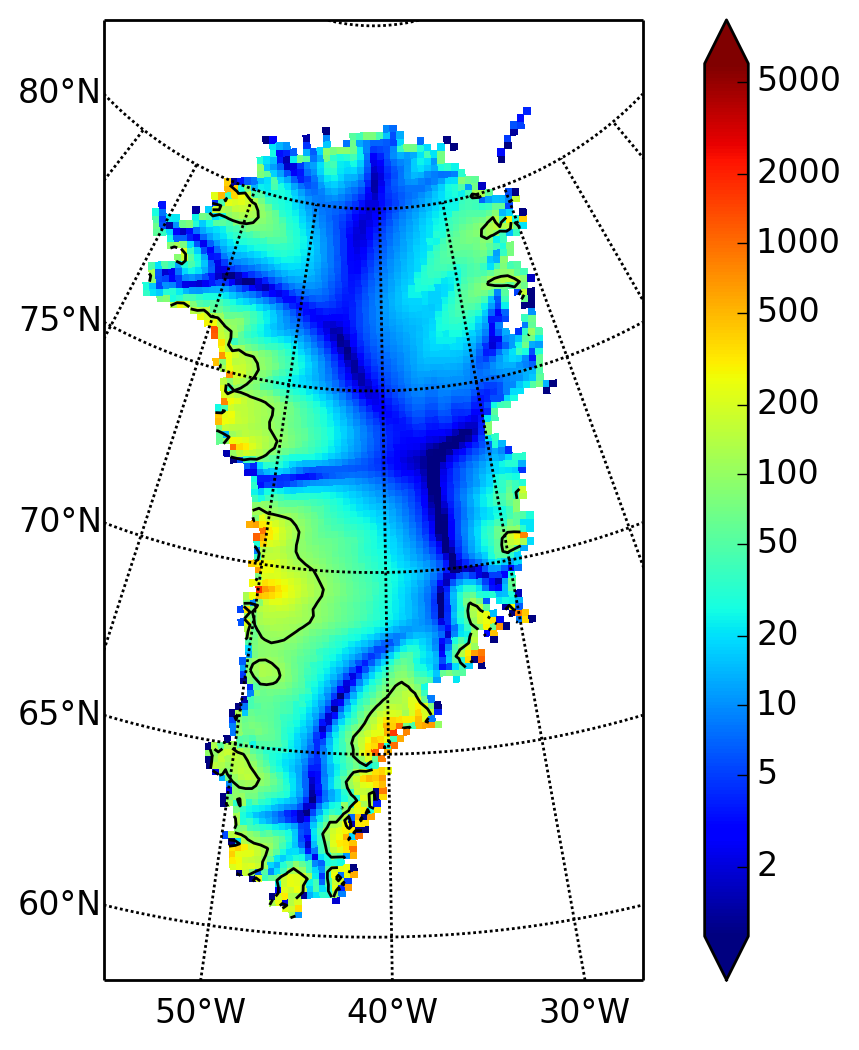
\includegraphics[height=2.75in,keepaspectratio=true]{g20km-10ka-hy-csurf} 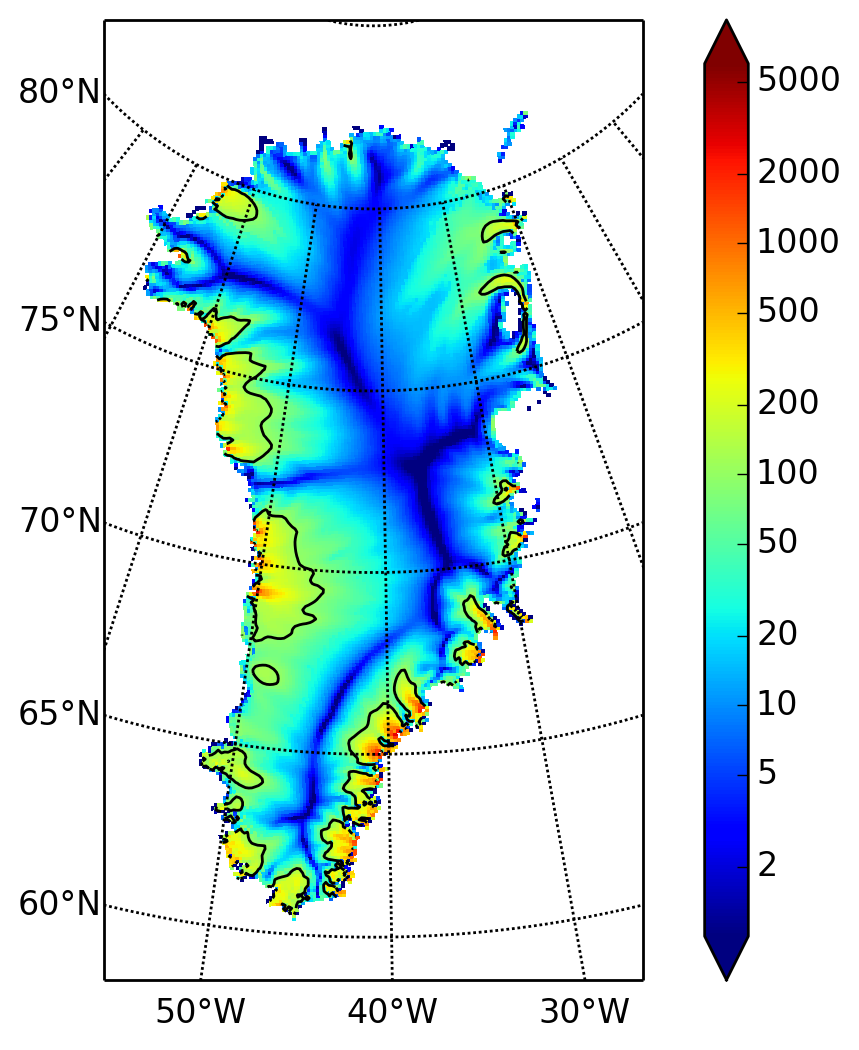
\includegraphics[height=2.75in,keepaspectratio=true]{g10km-10ka-hy-csurf}}
\caption{Comparing observed and modeled surface speed.  All figures have a common scale (m/a), with 100 m/a contour shown (solid black).  Left: \texttt{surfvelmag}, the observed values from SeaRISE data file \texttt{Greenland_5km_v1.1.nc}.  Middle: \texttt{csurf} from \texttt{g20km_10ka_hy.nc}.  Right: \texttt{csurf} from \texttt{g10km_10ka_hy.nc}.}
\label{fig:csurfvsobserved}
\end{figure}

The reader might agree with these broad qualitative judgements:
\begin{itemize}
\item the model results and the observed surface velocity look similar, but
\item the slow flow near the divide is generally in the right areas and of generally the right magnitude, and
\item the observed Northeast Greenland ice stream is much more distinct in observations than in the model.
\end{itemize}

We can compare these easily-generated PISM results to some recent observed-vs-model comparisons of surface velocity maps, of exactly this type, for example Figure 1 in \cite{Priceetal2011} and Figure 8 in \cite{Larouretal2012}.  Note that only ice-sheet-wide parameters and models were used here in PISM, that is, each location in the ice sheet was modeled by the same physics.  By comparison, those published comparisons involved tuning a large number of subglacial parameters to values which would yield close match to observations of the surface velocity.  Such tuning techniques are usually called ``inversion'' or ``assimilation'' of the surface velocity data.  Such methods are also possible in PISM if desired,\footnote{See \cite{vanPeltetal2013} (inversion of DEMs for basal topography) and \cite{Habermannetal2013} (inversion surface velocities for basal shear stress) for PISM-based inversion methods and analysis.} but the advantage of having few parameters in a model is well-known: the results reflect the underlying model not the flexibility of fitting many parameters.

Of course, we have only tried two of the many models possible in PISM.  We are free to identify and adjust important parameters.  The first parameter change we consider, in the next subsection, is one of the most important: grid resolution.


\subsection{Third run: higher resolution}  \label{subsect:higherresrun}

Now we change one key parameter, the grid resolution.  If you can let it run overnight, do
\begin{verbatim}
$ PARAM_PPQ=0.5 ./spinup.sh 4 const 10000 10 hybrid g10km_10ka_hy.nc &> out.g10km_10ka_hy &
\end{verbatim}
This run might take 4 to 6 hours.  However, supposing you have a larger parallel computer, you can change ``\texttt{mpiexec -n 4}'' to ``\texttt{mpiexec -n N}'' where \texttt{N} is a substantially larger number, up to 100 or so with an expectation of reasonable scaling on this grid \cite{BBssasliding,DickensMorey2013}.

Some fields from the result \verb|g10km_10ka_hy.nc| are shown in Figure \ref{fig:secondoutputfiner}.  Figure \ref{fig:csurfvsobserved} also compares observed velocity to the model results from 20 km and 10 km grids.  Model results differ even when the only change is the resolution!  Importantly for ice sheet modeling, using higher resolution ``picks up'' more detail in the bed elevation and climate data.

\begin{figure}[ht]
\centering
\mbox{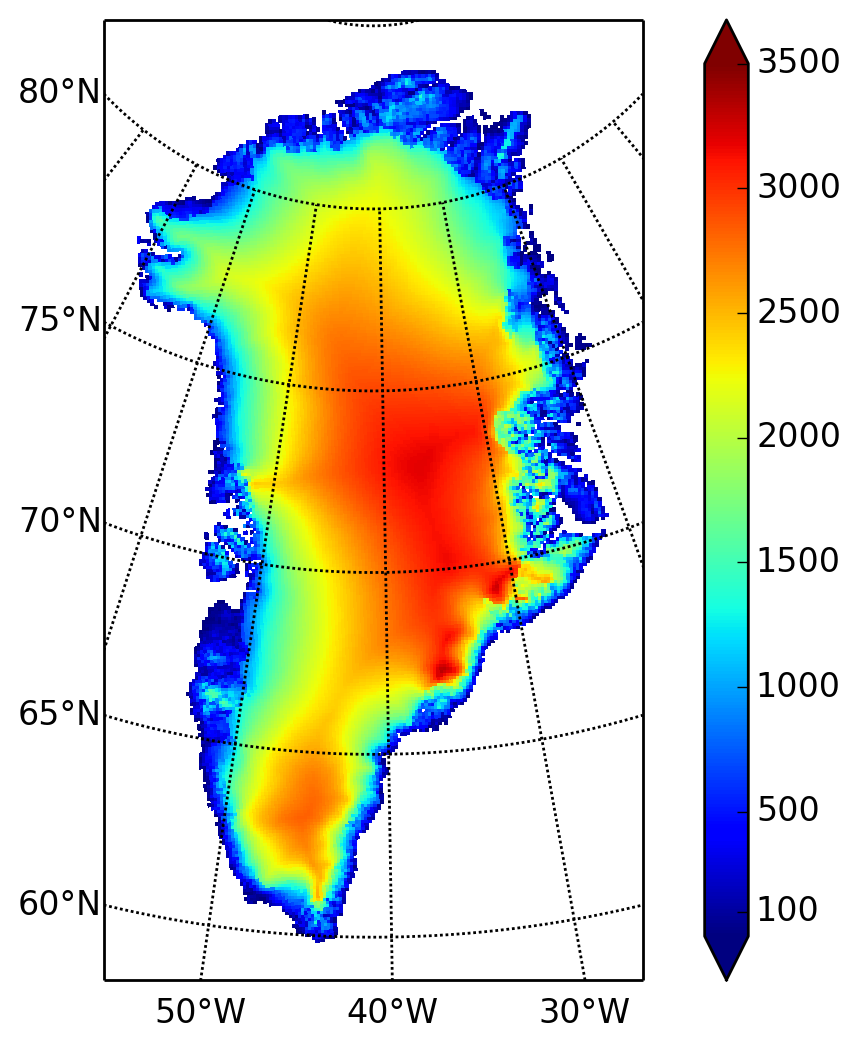
\includegraphics[height=2.75in,keepaspectratio=true]{g10km-10ka-hy-usurf} 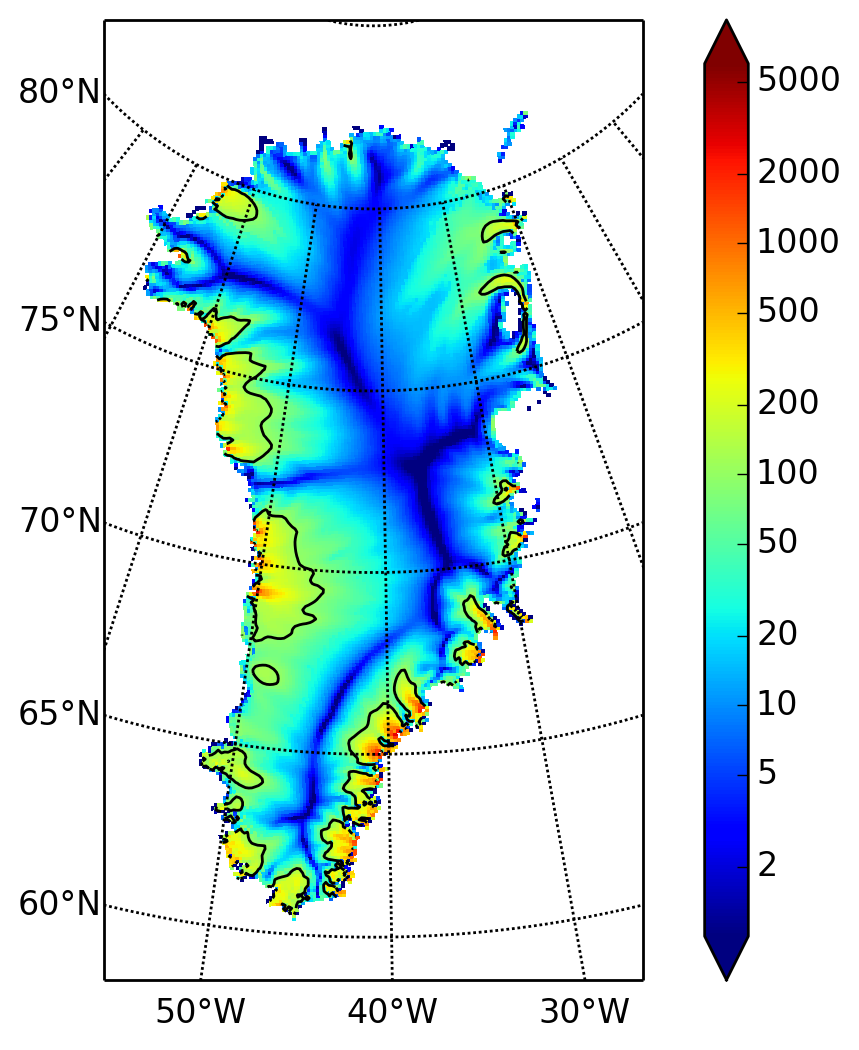
\includegraphics[height=2.75in,keepaspectratio=true]{g10km-10ka-hy-csurf} 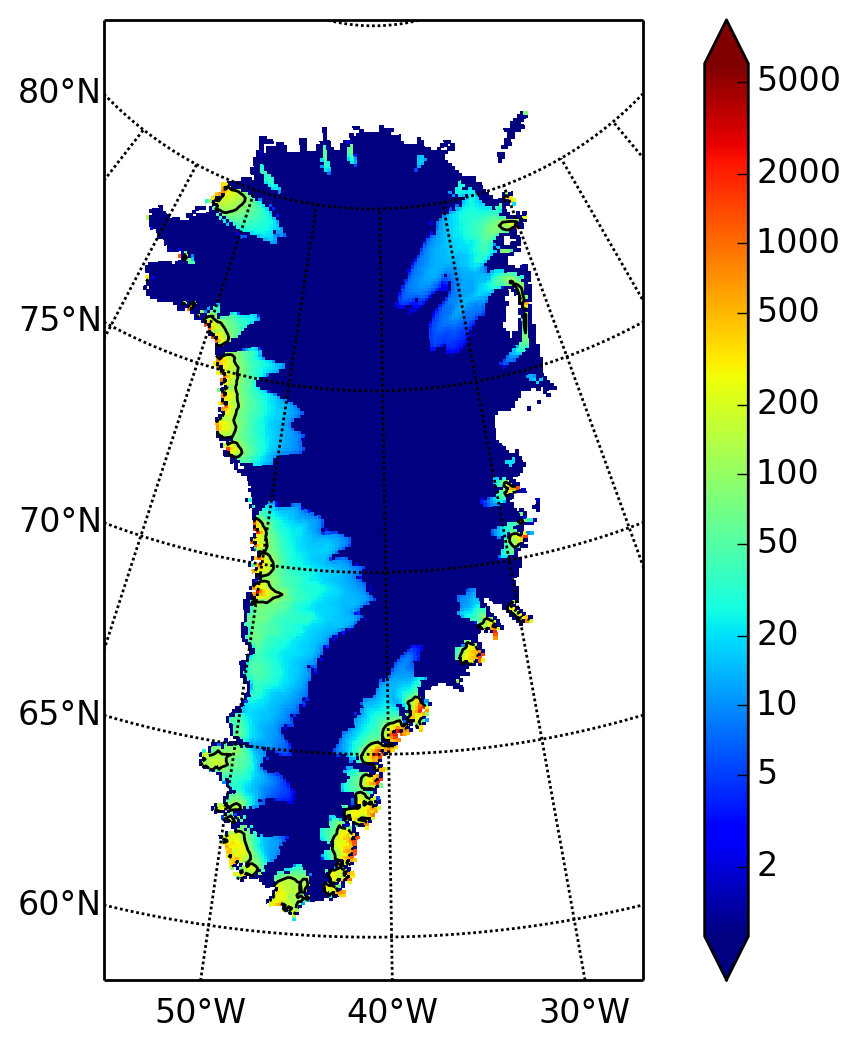
\includegraphics[height=2.75in,keepaspectratio=true]{g10km-10ka-hy-cbase}}
\caption{Fields from output file \texttt{g10km_10ka_hy.nc}.  Compare Figure \ref{fig:secondoutputcoarse}, which only differs by resolution.  Left: \texttt{usurf} in meters.  Middle: \texttt{csurf} in m/a.  Right: \texttt{cbase} in m/a.}
\label{fig:secondoutputfiner}
\end{figure}

As a different kind of comparison, Figure \ref{fig:ivolboth} shows ice volume time series \texttt{ivol} for 20km and 10km runs done here.  We see that this result depends on resolution, in particular because higher resolution grids allow the model to better resolve the flux through topographically-controlled outlet glaciers (compare \cite{Pfefferetal2008}).  However, because the total ice sheet volume is a highly-averaged quantity, the \texttt{ivol} difference from 20km and 10km resolution runs is only about one part in 60 (about 1.5\%) at the final time.  By contrast, as is seen in the near-margin ice in various locations shown in Figure \ref{fig:csurfvsobserved}, the ice velocity at a particular location may change by 100\% when the resolution changes from 20km to 10km.

Roughly speaking, the reader should only consider trusting those model results which are demonstrated to be robust across a range of model parameters, and, in particular, which are shown to be relatively-stable among relatively-high resolution results for a particular case.  Using a supercomputer is justified merely to confirm that lower-resolution runs were already ``getting'' a given feature!

\begin{figure}[ht]
\centering
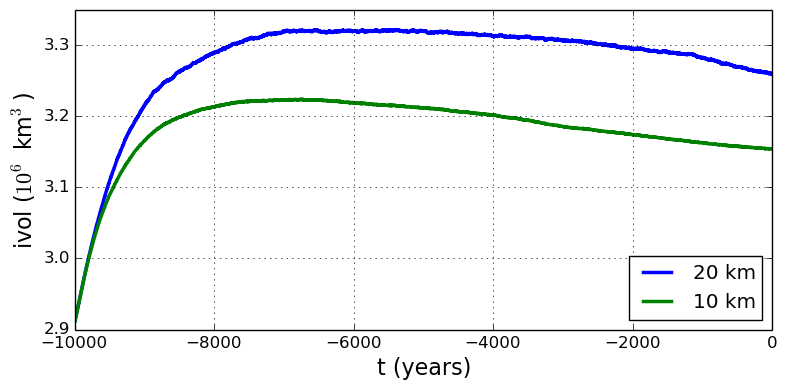
\includegraphics[width=4.0in,keepaspectratio=true]{ivol-both-g20km-g10km}
\caption{Time series of modeled ice sheet volume \texttt{ivol} on 20km and 10km grids.  The present-day ice sheet has volume about $2.9\times 10^6\,\text{km}^3$ \cite{BamberLayberryGogenini}, the initial value seen in both runs.}
\label{fig:ivolboth}
\end{figure}


\subsection{Fourth run: paleo-climate model spin-up}  \label{subsect:paleorun}  

A this point we have barely mentioned one of the most important players in the ice sheet modeling game: the surface mass balance (SMB) model.  Specifically, an SMB model combines precipitation (e.g.~\cite{Balesetal2001} for present-day Greenland) and a model for melt.  Melt models are always based on some approximation of the energy available at the ice surface \cite{Hock05}.  Previous runs in this section used a ``constant-climate'' assumption, which specifically meant using the modeled present-day SMB rates from the regional climate model RACMO \cite{Ettemaetal2009}, as contained in the SeaRISE-Greenland data set \verb|Greenland_5km_v1.1.nc|.

While a physical model of ice dynamics only describes the movement of the ice, the SMB (and the sub-shelf melt rate) are key inputs which directly determine changes in the boundary geometry.  Boundary geometry changes then feedback to determine the stresses seen by the stress balance and thus the motion.

There are other methods for producing SMB than to use present-day modeled values.  We now try such a method, a ``paleo-climate spin-up'' for our Greenland ice sheet model.  Of course, direct measurements of prior climates in Greenland are not available as data!  There are, however, estimates of past surface temperatures at the locations of ice cores \cite[for GRIP]{JohnsenetalGRIP}, along with estimates of past global sea level \cite{Imbrieetal1984} which can be used to determine where the flotation criterion is applied---this is how PISM's \verb|mask| variable is determined.  Also, models have been constructed for how precipitation differs from the present-day values \cite{Huybrechts02}.  For demonstration purposes, these are all used in the next run.  The relevant options are further documented in PISM's Climate Forcing Manual.

As noted, one must compute melt in order to compute SMB.  This is done using a temperature-index, ``positive degree-day'' (PDD) model \cite{Hock05}.  Such a PDD model has parameters for how much snow and/or ice is melted when surface temperatures spend time near or above zero degrees.  Again, see the PISM Climate Forcing Manual for relevant options.

To summarize the paleo-climate model applied here, temperature offsets from the GRIP core record affect the snow energy balance, and thus the rates of melting and runoff calculated by the PDD model.  In warm periods there is more marginal ablation, but precipitation may also increase (according to a temperature-offset model \cite{Huybrechts02}).  Additionally sea level undergoes changes in time and this affects which ice is floating.  Finally we add an earth deformation model, which responds to changes in ice load by changing the bedrock elevation \cite{BLKfastearth}.

To see how all this translates into PISM options, do
\begin{verbatim}
$ PISM_DO=echo PARAM_PPQ=0.5 REGRIDFILE=g20km_10ka_hy.nc \
  ./spinup.sh 4 paleo 25000 20 hybrid g20km_25ka_paleo.nc
\end{verbatim}

\begin{figure}[ht]
\centering
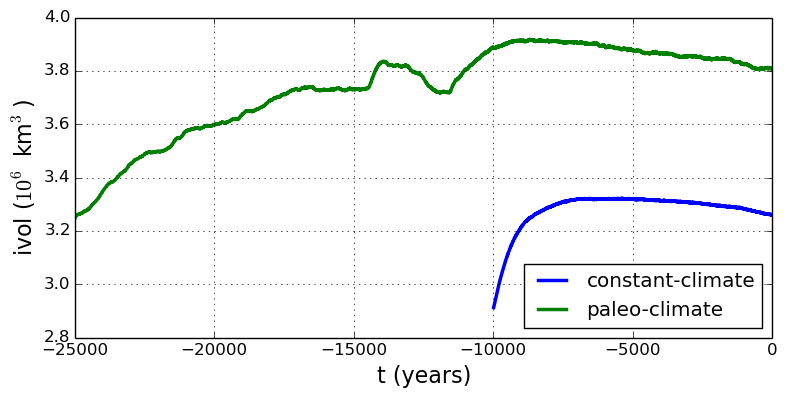
\includegraphics[width=4.5in,keepaspectratio=true]{ivol-const-paleo}
\caption{Time series of modeled ice sheet volume \texttt{ivol} from constant-climate (blue; \texttt{ts_g20km_10ka_hy.nc}) and paleo-climate (red; \texttt{ts_g20km_25ka_paleo.nc}) spinup runs.  Note that the paleo-climate run started with the ice geometry at the end of the constant-climate run.}
\label{fig:ivolconstpaleo}
\end{figure}

You will see an impressive command, which you can compare to the one on page \pageref{firstcommand}.  There are several key changes.  First, we do not start from scratch but instead from a previously computed near-equilibrium result:
\begin{verbatim}
  -regrid_file g20km_10ka_hy.nc -regrid_vars litho_temp,thk,enthalpy,tillwat,bmelt
\end{verbatim}
For more on regridding see subsection \ref{sec:regridding}.  Then we turn on the earth deformation model with option \verb|-bed_def lc|; see subsection \ref{subsect:beddef}.  After that the atmosphere and surface (PDD) models are turned on and the files they need are identified:
\begin{verbatim}
  -atmosphere searise_greenland,delta_T,paleo_precip -surface pdd \
  -atmosphere_paleo_precip_file pism_dT.nc -atmosphere_delta_T_file pism_dT.nc
\end{verbatim}
Then the ocean model, which provides both a subshelf melt rate and a time-dependent sealevel to the ice dynamics core, is turned on with \verb|-ocean constant,delta_SL| and the file it needs is identified with \verb|-ocean_delta_SL_file pism_dSL.nc|.  For all of these ``forcing'' options, see the PISM Climate Forcing Manual.  The remainder of the options are similar or identical to the run that created \verb|g20km_10ka_hy.nc|.

To actually start the run, which we rather arbitrarily start at year -25000, essentially at the LGM, do:
\begin{verbatim}
$ PARAM_PPQ=0.5 REGRIDFILE=g20km_10ka_hy.nc \
  ./spinup.sh 4 paleo 25000 20 hybrid g20km_25ka_paleo.nc &> out.g20km_25ka_paleo &
\end{verbatim}
This run should only take one or two hours, noting it is at a coarse 20 km resolution.

The fields \texttt{usurf}, \texttt{csurf}, and \texttt{cbase} from file \texttt{g20km_25ka_paleo.nc} are sufficiently similar to those shown in Figure \ref{fig:secondoutputcoarse} that they are not shown here.  Close inspection reveals differences, but of course these runs only differ in the applied climate and run duration and not in resolution or ice dynamics parameters.

\begin{figure}[ht]
\centering
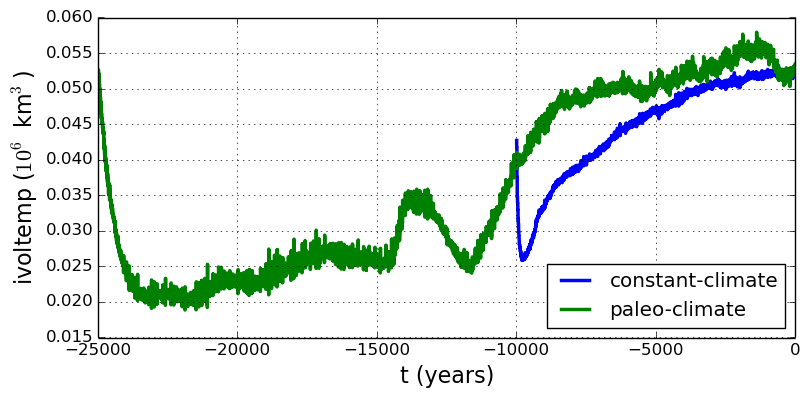
\includegraphics[width=4.5in,keepaspectratio=true]{ivoltemp-const-paleo}
\caption{Time series of temperate ice volume \texttt{ivoltemp} from constant-climate (blue; \texttt{ts_g20km_10ka_hy.nc}) and paleo-climate (red; \texttt{ts_g20km_25ka_paleo.nc}) spinup runs.  The cold of the last ice age affects the fraction of temperate ice.  Note different volume scale compared to that in Figure \ref{fig:ivolconstpaleo}; only about 1\% of ice is temperate (by volume).}
\label{fig:ivoltempconstpaleo}
\end{figure}

To see the difference between runs more clearly, Figure \ref{fig:ivolconstpaleo} compares the time-series variable \texttt{ivol}.  We see the effect of option \verb|-regrid_file g20km_10ka_hy.nc -regrid_vars ...,thk,...|, which implies that the paleo-climate run starts with the ice geometry from the end of the constant-climate run.

Another time-series comparison, of the variable \verb|ivoltemp|, the total volume of temperate (at 0$^\circ$C) ice, appears in Figure \ref{fig:ivoltempconstpaleo}.  The paleo-climate run shows the cold period from $\approx -25$ ka to $\approx -12$ ka.  Both constant-climate and paleo-climate runs then come into rough equilibrium in the holocene.  The bootstrapping artifact, seen at the start of the constant-climate run, which disappears in less than 1000 years, is avoided in the paleo-climate run by starting with the constant-climate end-state.  The reader is encouraged to examine the diagnostic files \texttt{ts_g20km_25ka_paleo.nc} and \texttt{ex_g20km_25ka_paleo.nc} to find more evidence of the (modeled) climate impact on the ice dynamics.


\subsection{Getting serious I: grid sequencing}  \label{subsect:gridseq}  

The previous sections were not very ambitious.  We were just getting started!  Now we demonstrate a serious PISM capability, the ability to change, specifically to \emph{refine}, the grid resolution at runtime.

One can of course do the longest model runs using a coarse grid, like the 20 km grid used first.  It is, however, only possible to pick up detail from high quality data, for instance bed elevation and/or high-resolution climate data, using high grid resolution.

Also, a 20 or 10 km grid is inadequate for resolving the flow of the ice sheet through the kind of fjord-like, few-kilometer-wide topographical confinement which occurs, for example, at Jakobshavn Isbrae in the west Greenland ice sheet \cite{Joughinetal08}, an important outlet glacier which both flows fast and drains a large fraction of the ice sheet.  One possibility is to set up an even higher-resolution PISM regional model covering only one outlet glacier, but this requires decisions about coupling to the whole ice sheet flow.  (See section \ref{sec:jako}.)  But let's work on high resolution for the whole ice sheet and all outlet glaciers.

Consider the following command; compare it to the one on page \pageref{firstcommand}:
\begin{verbatim}
mpiexec -n 4 pismr -boot_file pism_Greenland_5km_v1.1.nc -Mx 301 -My 561 \
  -Mz 201 -Mbz 21 -z_spacing equal -Lz 4000 -Lbz 2000 -ys -200 -ye 0 \
  -regrid_file g20km_10ka_hy.nc -regrid_vars litho_temp,thk,enthalpy,tillwat,bmelt ...
\end{verbatim}
Instead of a 20 km grid in the horizontal (\verb|-Mx 76 -My 141|) we ask for a 5 km grid (\verb|-Mx 301 -My 561|).  Instead of vertical grid resolution of 40 m (\verb|-Mz 101 -z_spacing equal -Lz 4000|) we ask for a vertical resolution of 20 m (\verb|-Mz 201 -z_spacing equal -Lz 4000|).\footnote{See subsections \ref{sec:bootstrapping}, \ref{subsect:coords}, and \ref{subsect:grid} for more about determining the computation domain and grid at bootstrapping.}  Most significantly, however, we say \verb|-regrid_file g20km_10ka_hy.nc| to regrid---specifically, to bilinearly-interpolate---fields from a model result computed on the coarser 20 km grid.  The regridded fields (\verb|-regrid_vars litho_temp,...|) are the evolving mass and energy state variables which are already approximately at equilibrium on the coarse grid.  Because we are bootstrapping (i.e.~using \verb|-boot_file|), the other variables, especially the bedrock topography \verb|topg| and the climate data, are brought in to PISM at ``full'' resolution, that is, on the original 5 km grid in the data file \texttt{pism_Greenland_5km_v1.1.nc}.

This technique could be called ``grid sequencing''.\footnote{It is not quite ``multigrid.''  That would both involve refinement and coarsening stages in computing the fine grid solution.}  The result of the above command will be to compute the near-equilibrium result on the fine 5 km grid, taking advantage of the coarse-gridded computation of approximate equilibrium, and despite a run of only 200 model years (\verb|-ys -200 -ye 0|).  How close to equilibrium we get depends on both durations, i.e.~on both the coarse and fine grid run durations, but certainly the computational effort is reduced by doing a short run on the fine grid.  Note that in the previous subsection we also used regridding.  In that application, however, \verb|-regrid_file| only ``brings in'' fields from a run on the same resolution.

Generally the fine grid run duration in grid sequencing should be at least $t = \Delta x / v_{\text{min}}$ where $\Delta x$ is the fine grid resolution and $v_{\text{min}}$ is the lowest ice flow speed that we expect to be relevant to our modeling purposes.  That is, the duration should be such that slow ice at least has a chance to cross one grid cell.  In this case, if $\Delta x = 5$ km and $v_{\text{min}} = 25$ m/a then we get $t=200$ a.  Though we use this as the duration, it is a bit short, and the reader might compare $t=500$ results (i.e.~using $v_{\text{min}} = 10$ m/a).

Of course there is no reason to jump from $20\,\text{km}$ to $5\,\text{km}$ in one step!  Instead we will do it in two steps, $20\,\text{km}\,\to\,10\,\text{km}\,\to\,5\,\text{km}$, with durations of 10 ka, 2 ka, and 200 a, respectively.  The 20 km coarse grid run is already done; the result is in \texttt{g20km_10ka_hy.nc}.  So we run the following script which is \texttt{gridseq.sh} in \texttt{examples/std-greenland/}.  It calls \texttt{spinup.sh} to collect all the right PISM options:
\begin{scriptvrb}
#!/bin/bash
NN=4
export PARAM_PPQ=0.5
export REGRIDFILE=g20km_10ka_hy.nc
export EXSTEP=100
./spinup.sh $NN const 2000  10 hybrid g10km_gridseq.nc
export REGRIDFILE=g10km_gridseq.nc
export EXSTEP=10
./spinup.sh $NN const 200    5 hybrid  g5km_gridseq.nc
\end{scriptvrb}
Environment variable \verb|EXSTEP| specifies the time in years between writing the spatially-dependent, and large-file-size-generating, frames for the \verb|-extra_file ...| diagnostic output.

Before you run the above script, however, an important

\medskip
\centerline{\large\underline{\emph{WARNING:} the 5km run requires 8 Gb of memory at minimum!}\normalsize}

\medskip
\noindent If you try it without at least 8 Gb of memory then your machine will ``bog down'' and start using the hard disk for swap space!  The run will not complete and your hard disk will get a lot of wear!  (If you have less than 8 Gb memory, comment out the last three lines of the above script---e.g.~using the ``\verb|#|'' character at the beginning of the line---so that you only do the 20 km $\to$ 10 km refinement.)

Run the script like this:
\begin{verbatim}
$ ./gridseq.sh &> out.gridseq &
\end{verbatim}
The 10 km run takes under two hour and the 5 km run takes under four hours.

\begin{figure}[ht]
\centering
\mbox{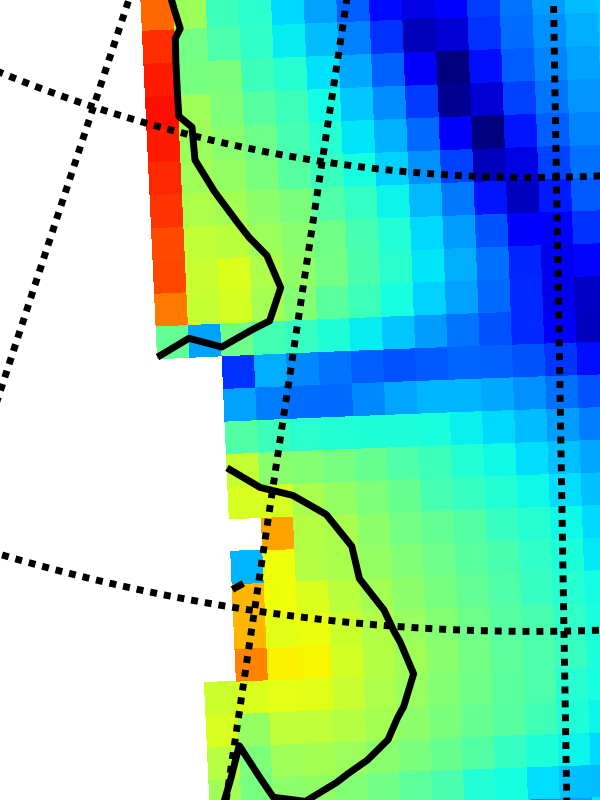
\includegraphics[width=1.65in,keepaspectratio=true]{g40km-detail} 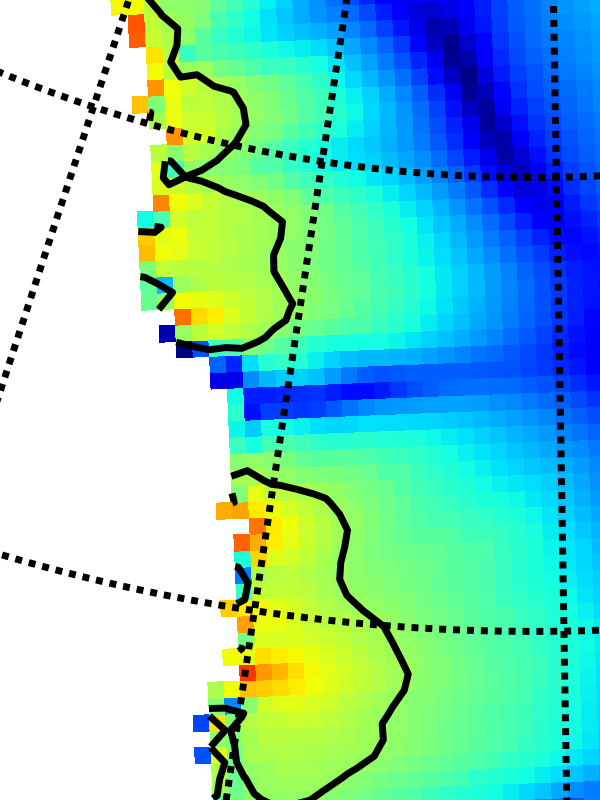
\includegraphics[width=1.65in,keepaspectratio=true]{g20km-detail} 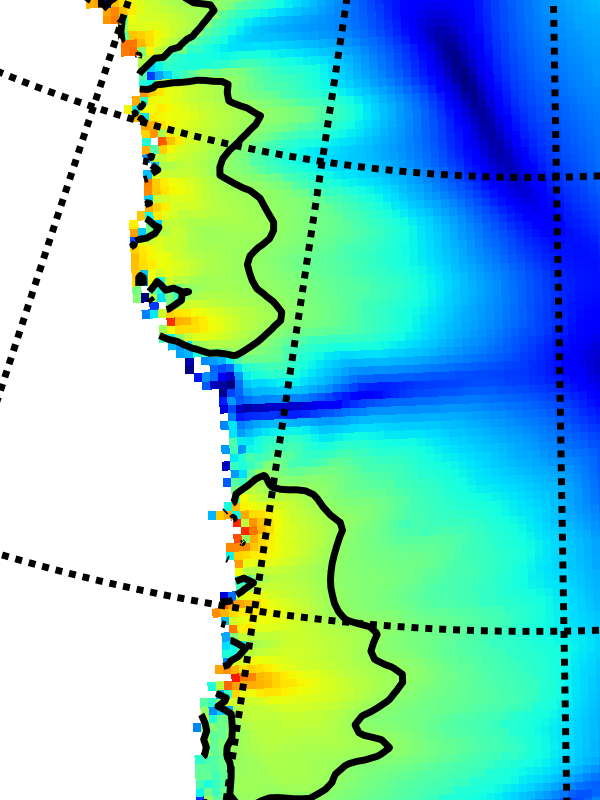
\includegraphics[width=1.65in,keepaspectratio=true]{g10km-detail} 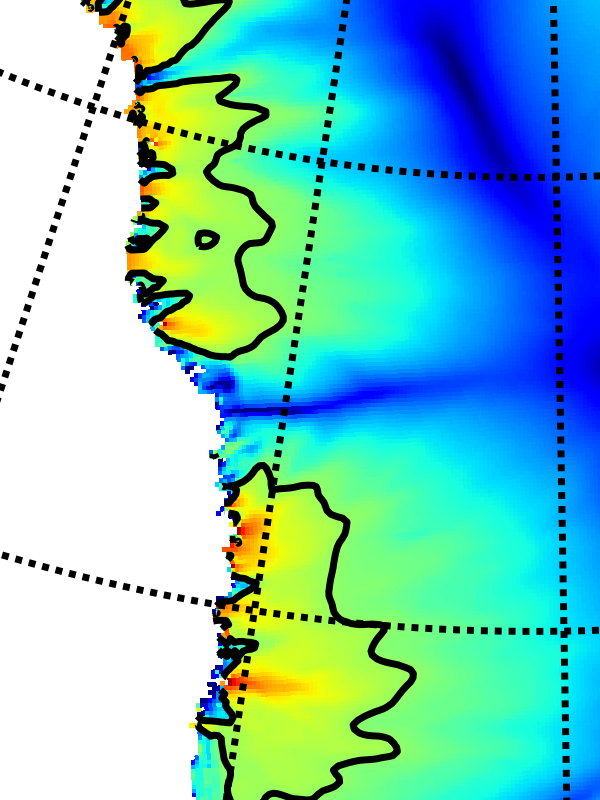
\includegraphics[width=1.65in,keepaspectratio=true]{g5km-detail} }
\caption{Detail of field \texttt{csurf} showing the central western coast of Greenland, including Jakobshavn Isbrae (lowest major flow), from runs of resolution 40, 20, 10, 5 km (left-to-right).  Color scheme and scale, including 100 m/a contour (solid black), are all identical to \texttt{csurf} Figures \ref{fig:secondoutputcoarse}, \ref{fig:csurfvsobserved}, and \ref{fig:secondoutputfiner}.}
\label{fig:gridseqdetail}
\end{figure}

Figure \ref{fig:gridseqdetail}, showing only a detail of the western coast of Greenland, with several outlet glaciers visible, suggests what is accomplished: the high resolution runs have separated outlet glacier flows, as they are in fact.  Note that all of these results were generated in a few wall clock hours on a laptop!  The surface speed \texttt{csurf} from files \texttt{g10km_gridseq.nc} and \texttt{g5km_gridseq.nc} is shown (two right-most subfigures).  In the two left-hand subfigures we show the same field from NetCDF files \texttt{g40km_10ka_hy.nc} and \texttt{g20km_10ka_hy.nc}; the former is an added 40 km result using an obvious modification of the run in section \ref{subsect:ssarun}.

\begin{figure}[ht]
\centering
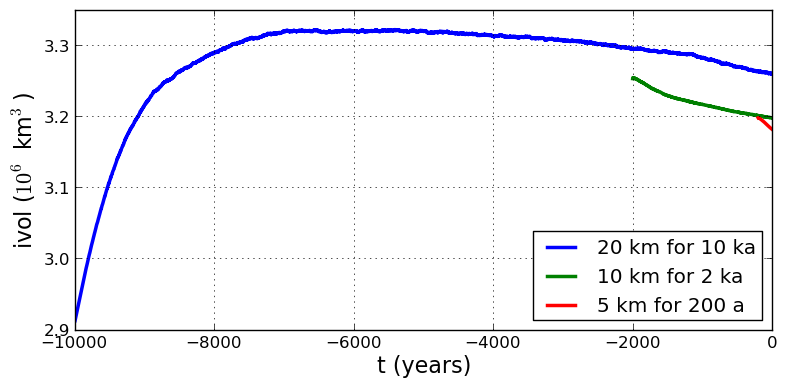
\includegraphics[width=4.5in,keepaspectratio=true]{ivol-gridseq}
\caption{Time series of ice volume \texttt{ivol} from the three runs in our grid sequencing example: 20 km for 10 ka = \texttt{ts_g20km_10ka_hy.nc}, 10 km for 2 ka = \texttt{ts_g10km_gridseq.nc}, and 5 km for 200 a = \texttt{ts_g20km_10ka_hy.nc}.}
\label{fig:ivolgridseq}
\end{figure}

Figure \ref{fig:ivolgridseq}, which shows time series of ice volume, also shows the cost of high resolution, however.  The short 200 a run on the 5 km grid took about 3 wall-clock hours compared to the 10 minutes taken by the 10 ka run on a 20 km grid.  The fact that the time series for ice volume on 10 km and 5 km grids are not very ``steady'' also suggests that these runs should actually be longer.

In this vein, if you have an available supercomputer then a good exercise is to extend our grid sequencing example to 3 km or 2 km resolutions \cite{AschwandenAdalgeirsdottirKhroulev}; these grids are already supported in the script \texttt{spinup.sh}.  Note that the vertical grid also generally gets refined as the horizontal grid is refined.

Going to a 1km grid is possible, but you will start to see the limitations of distributed file systems in writing the enormous NetCDF files in question \cite{DickensMorey2013}.  Notice that a factor-of-five refinement in all three dimensions, e.g.~from 5 km to 1 km in the horizontal, and from 20 m to 4 m in the vertical, generates an output NetCDF file which is 125 times larger.  Since the already-generated 5 km result \texttt{g5km_gridseq.nc} is over 0.5 Gb, the result is a very large file at 1 km.

On the other hand, on fine grids we observe that \emph{memory} parallelism, i.e.~spreading the stored model state over the separated memory of many nodes of supercomputers, is as important as the usual \emph{computation} (CPU) parallelism.

This subsection has emphasized the ``P'' in PISM, the nontrivial parallelism in which the solution of the conservation equations, especially the stress balance equations, is distributed across processors.  An easier and more common mode of parallelism is to distribute distinct model runs, each with different parameter values, among the processors.  For scientific purposes, such parameter studies, whether parallel or not, are at least as valuable as individual high-resolution runs.


\subsection{Getting serious II: an ice dynamics parameter study}  \label{subsect:paramstudy}

The readers of this manual should not assume the PISM authors know all the correct parameters for describing ice flow.  While PISM must have \emph{default} values of all parameters, to help users get started,\footnote{They are stored in human-readable form in the file \texttt{src/pism_config.cdl}.} it has more than two hundred user-configurable parameters.  The goal in this manual is to help the reader adjust them to their desired values.  While ``correct'' values may never be known, or may not exist, examining the behavior of the model as it depends on parameters is both a nontrivial and an essential task.

For some parameters used by PISM, changing their values within their ranges of experimental uncertainty is unlikely to affect model results in any important manner (e.g.~\texttt{sea_water_density}).  For others, however, for instance for the exponent in the basal sliding law, changing the value is highly-significant to model results, as we'll see in this subsection.  This is also a parameter which is very uncertain given current glaciological understanding \cite{CuffeyPaterson}.

To illustrate a parameter study in this Manual we restrict consideration to just two important parameters for ice dynamics,\begin{itemize}
\item $q=$ \texttt{pseudo_plastic_q}: exponent used in the sliding law which relates basal sliding velocity to basal shear stress in the SSA stress balance; see subsection \ref{subsect:basestrength} for more on this parameter, and
\item $e=$ \texttt{sia_enhancement_factor}: values larger than one give flow ``enhancement'' by making the ice deform more easily in shear than is determined by the standard flow law \cite{LliboutryDuval1985,PatersonBudd}; applied only in the SIA stress balance; see subsection \ref{sec:rheology} for more on this parameter.
\end{itemize}

By varying these parameters over full intervals of values, say $0.1\le q \le 1.0$ and $1 \le e \le 6$, we could explore a two-dimensional parameter space.  But of course each $(q,e)$ pair needs a full computation, so we can only sample this two-dimensional space.  Furthermore we must specify a concrete run for each parameter pair.  In this case we choose to run for 1000 model years, in every case initializing from the stored state \texttt{g10km_gridseq.nc} generated in the previous subsection \ref{subsect:gridseq}.

The next script, which is \texttt{param.sh} in \texttt{examples/std-greenland/}, gets values $q\in\{0.1,0.5,1.0\}$ and $e\in\{1,3,6\}$ in a double \texttt{for}-loop.  It generates a run-script for each $(q,e)$ pair.  For each parameter setting it calls \texttt{spinup.sh}, with the environment variable \texttt{PISM_DO=echo} so that \texttt{spinup.sh} simply outputs the run command.  This run command is then redirected into an appropriately-named \texttt{.sh} script file:
\begin{scriptvrb}
#!/bin/bash
NN=4
DUR=1000
START=g10km_gridseq.nc
for PPQ in 0.1 0.5 1.0 ; do
  for SIAE in 1 3 6 ; do
     PISM_DO=echo REGRIDFILE=$START PARAM_PPQ=$PPQ PARAM_SIAE=$SIAE \
       ./spinup.sh $NN const $DUR 10 hybrid p10km_${PPQ}_${SIAE}.nc \
       &> p10km_${PPQ}_${SIAE}.sh
  done
done
\end{scriptvrb}
%$
Notice that, because the stored state \texttt{g10km_gridseq.nc} used $q=0.5$ and $e=3$, one of these runs simply  continues with no change in the physics.

To set up and run the parameter study, without making a mess from all the generated files, do:
\small
\begin{verbatim}
$ cd examples/std-greenland/           # g10km_gridseq.nc should be in this directory
$ mkdir paramstudy
$ cd paramstudy
$ ln -s ../g10km_gridseq.nc            # these four lines make links to ...
$ ln -s ../pism_Greenland_5km_v1.1.nc  #
$ ln -s ../spinup.sh                   #
$ ln -s ../param.sh                    # ... existing files in examples/std-greenland/
$ ./param.sh
\end{verbatim}
\normalsize
The result of the last command is to generate nine run scripts,
\small
\begin{verbatim}
p10km_0.1_1.sh  p10km_0.1_3.sh  p10km_0.1_6.sh
p10km_0.5_1.sh  p10km_0.5_3.sh  p10km_0.5_6.sh
p10km_1.0_1.sh  p10km_1.0_3.sh  p10km_1.0_6.sh
\end{verbatim}
\normalsize
The reader should inspect a few of these scripts.  They are all very similar, of course, but, for instance, the \texttt{p10km_0.1_1.sh} script uses options \texttt{-pseudo_plastic_q 0.1} and \texttt{-sia_e 1}.

\begin{figure}[ht]
\centering
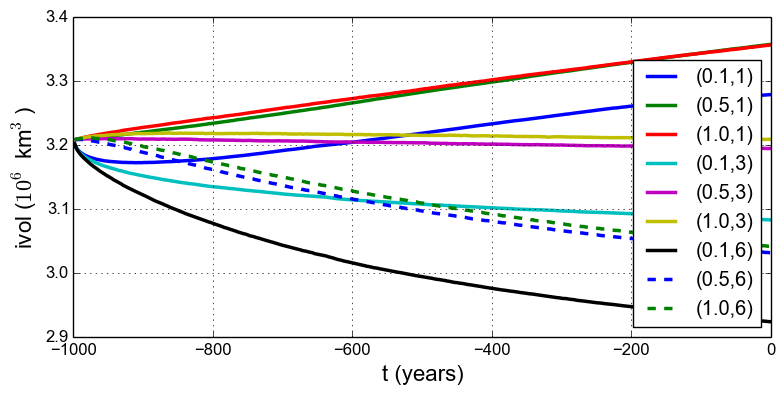
\includegraphics[width=4.5in,keepaspectratio=true]{ivol-param}

\caption{Time series of ice volume \texttt{ivol} from nine runs in our parameter study example, with parameter choices $(q,e)$ given.}
\label{fig:ivolparamstudy}
\end{figure}

We have not yet run PISM, but only asked one script to create nine others.  We now have the option of running them sequentially or in parallel.  Each script itself does a parallel run, over the \texttt{NN=4} processes specified by \texttt{param.sh} when generating the run scripts.  If you have $4 \times 9 = 36$ cores available then you can do the runs fully in parallel (this is \texttt{runparallel.sh} in \texttt{examples/std-greenland/}):
\begin{scriptvrb}
#!/bin/bash
for scriptname in $(ls p10km*sh) ; do
  echo ; echo "starting ${scriptname} ..."
  bash $scriptname &> out.$scriptname &  # start immediately in background
done
\end{scriptvrb}
%$
Otherwise you should do them in sequence (this is \texttt{runsequential.sh} in \texttt{examples/std-greenland/}):
\begin{scriptvrb}
#!/bin/bash
for scriptname in $(ls p10km*sh) ; do
  echo ; echo "starting ${scriptname} ..."
  bash $scriptname                       # will wait for completion
done
\end{scriptvrb}
%$
On the same old 2012-era 4 core laptop, \texttt{runsequential.sh} took a total of just under 7 hours to complete the whole parameter study.  The runs with $q=0.1$ (the more ``plastic'' end of the basal sliding spectrum) took up to four times longer than the $q=0.5$ and $q=1.0$ runs.  Roughly speaking, values of $q$ which are close to zero imply a subglacial till model with a true yield stres, and the result is that even small changes in overall ice sheet state (geometry, energy, \dots) will cause \emph{some} location to exceed its yield stress and suddenly change flow regime.  This will shorten the time steps.  By contrast, the $e$ value is much less significant in determining run times.

\begin{figure}[ht]
\centering
\mbox{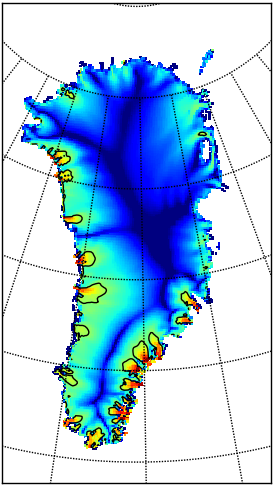
\includegraphics[height=2.6in,keepaspectratio=true]{p10km-01-1-csurf.png} 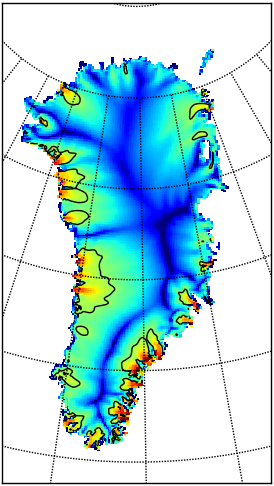
\includegraphics[height=2.6in,keepaspectratio=true]{p10km-01-3-csurf.png} 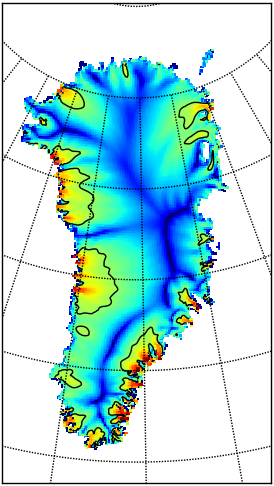
\includegraphics[height=2.6in,keepaspectratio=true]{p10km-01-6-csurf.png} \qquad \hspace{1.87in}}

\mbox{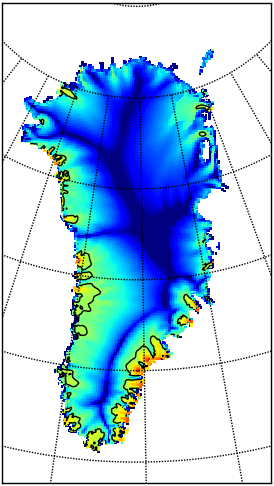
\includegraphics[height=2.6in,keepaspectratio=true]{p10km-05-1-csurf.png} 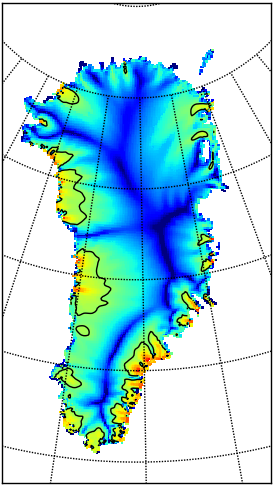
\includegraphics[height=2.6in,keepaspectratio=true]{p10km-05-3-csurf.png} 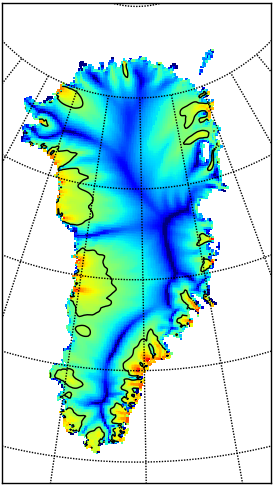
\includegraphics[height=2.6in,keepaspectratio=true]{p10km-05-6-csurf.png} 
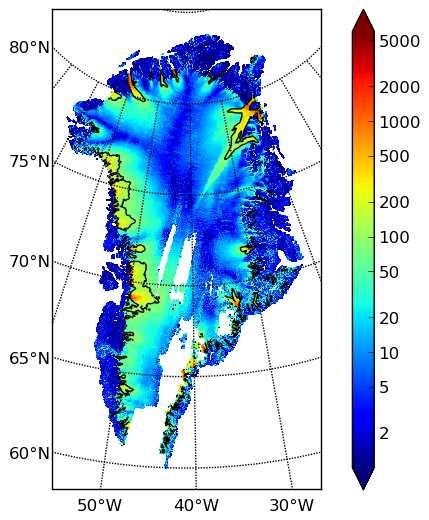
\includegraphics[height=2.7in,keepaspectratio=true]{Greenland-5km-v1p1-surfvelmag}}
\smallskip

\mbox{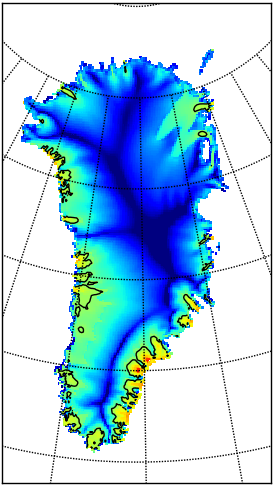
\includegraphics[height=2.6in,keepaspectratio=true]{p10km-1-1-csurf.png} 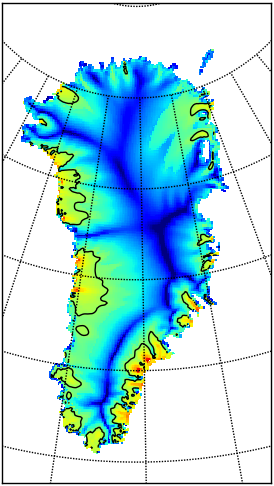
\includegraphics[height=2.6in,keepaspectratio=true]{p10km-1-3-csurf.png} 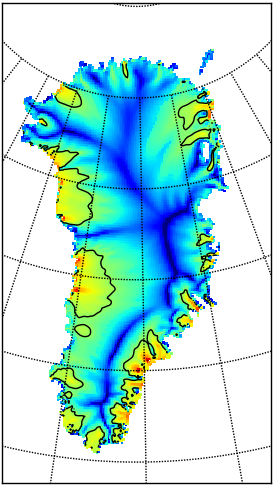
\includegraphics[height=2.6in,keepaspectratio=true]{p10km-1-6-csurf.png} \qquad \hspace{1.87in}}

\caption{Surface speed \texttt{csurf} from a 10 km grid parameter study.  Right-most subfigure is observed data from \texttt{Greenland_5km_v1.1.nc}.  Top row: $q=0.1$ and $e=1,3,6$ (left-to-right).  Middle row: $q=0.5$.  Bottom row: $q=1.0$.  All subfigures have common color scale (velocity m/a), as shown in the right-most figure, with 100 m/a contour shown in all cases (solid black).}
\label{fig:paramstudy}
\end{figure}

On a supercomputer, the \texttt{runparallel.sh} script generally should be modified to submit jobs to the scheduler.  See example scripts \texttt{advanced/paramspawn.sh} and \texttt{advanced/paramsubmit.sh} for a parameter study that does this.  (But see your system administrator if you don't know what a ``job scheduler'' is!)  Of course, if you have a supercomputer then you can redo this parameter study on a 5 km grid.

Results from these runs are seen in Figures \ref{fig:ivolparamstudy} and \ref{fig:paramstudy}.  In the former we see that the $(0.5,3)$ run simply continues the previous initialization run.  In some other graphs we see abrupt initial changes, caused by abrupt parameter change, e.g.~when the basal sliding becomes much more plastic ($q=0.1$).  In all cases with $e=1$ the flow slows and the sheet grows in volume as discharge decreases, while in all cases with $e=6$ the flow accelerates and the sheet shrinks in volume as discharge increases.

In Figure \ref{fig:paramstudy} we can compare the surface speed model results to observations.  Roughly speaking, the ice softness parameter $e$ has effects seen most-clearly by comparing the interior of the ice sheet; scan left-to-right for the $e=1,3,6$ subfigures.  The basal sliding exponent $q$ has effects seen most-clearly by comparing flow along the very steep margin, especially in the southern half of the ice sheet; scan top-to-bottom for $q=0.1,0.5,1.0$, going from nearly-plastic at top to linear at bottom.

From such figures we can make an informal assessment and comparison of the results, but objective assessment is important.  Example objective functionals include: \emph{(i)} compute the integral of the square (or other power) of the difference between the model and observed surface velocity \cite{AschwandenAdalgeirsdottirKhroulev}, or \emph{(ii)} compute the model-observed differences between the histogram of the number of cells with a given surface speed \cite{BKAJS}.  Note that these functionals are measuring the effects of changing a small number of parameters, namely two parameters in the current study.  So-called ``inversion'' might use the same objective functionals but with a much larger parameter space.  Inversion is therefore capable of achieving much smaller objective measures \cite{Habermannetal2013,Larouretal2012,Priceetal2011}, though at the cost of less understanding, perhaps, of the meaning of the optimal parameter values.

\clearpage  % does not lengthen pages, and puts Figure \ref{fig:paramstudy} before Table \ref{tab:NetCDFview}

\subsection{Handling NetCDF files}\label{subsect:nctoolsintro}  PISM takes one or more NetCDF files as input, then it does some computation, and then it produces one or more NetCDF files as output.  Usually, other tools help to extract meaning from these NetCDF files, and yet more tools help with creating PISM input files or post-processing PISM output files.  Thus we conclude this Getting Started section with a list of some NetCDF tools in Table \ref{tab:NetCDFview}.

We frequently use \texttt{ncview} and ``\texttt{ncdump -h}'' for quick visualization and metadata examination.  NCO has powerful command-line manipulation of NetCDF files, but requires some learning.  Often python scripts (using the \texttt{netcdf4-python} package; see the PISM Installation Manual), or Matlab or other languages, are the fastest way to fix up a NetCDF file or extract fields from it.  To use CDO on PISM files, first run the script \texttt{nc2cdo.py}, from the \texttt{util/} PISM directory, on the file.  This fixes the metadata so that CDO will understand the mapping.

See Table \ref{tab:modelhierarchy} in subsection \ref{sec:model-hierarchy} for an overview on the data necessary for modeling.  For more information on the format of input files for PISM, see section \ref{sec:initboot}.

\newcommand{\netcdftool}[1]{#1\index{NetCDF!tools!#1}}
\begin{table}[ht]
\centering
\small
\begin{tabular}{llp{0.45\linewidth}}
  \toprule
  \textbf{Tool} & \textbf{Site} & \textbf{Function} \\
  \midrule
  & \url{www.unidata.ucar.edu/software/netcdf/} & root for NetCDF information \\
  \midrule
  \netcdftool{\texttt{ncdump}} & \emph{included with any NetCDF distribution} & dump binary NetCDF as \texttt{.cdl} (text) file \\
  \netcdftool{\texttt{ncgen}} & \emph{included with any NetCDF distribution} & convert \texttt{.cdl} file to binary NetCDF \\
  \midrule
  \netcdftool{CDO} & \url{http://code.zmaw.de/projects/cdo} & = Climate Data Operators; command-line tools, including conservative re-mapping \\
  \netcdftool{IDV} & \url{http://www.unidata.ucar.edu/software/idv/} & more complete visualization \\
  \netcdftool{NCO}\index{NCO (NetCDF Operators)} & \url{http://nco.sourceforge.net/} & = NetCDF Operators; command-line tools\\
  \netcdftool{NCL} &  \url{http://www.ncl.ucar.edu} & = NCAR Command Language\\
  \netcdftool{\texttt{ncview}} & \href{http://meteora.ucsd.edu/~pierce/ncview_home_page.html}{\texttt{meteora.ucsd.edu/$\sim$pierce}} & quick graphical view \\
  \netcdftool{PyNGL} &  \url{http://www.pyngl.ucar.edu} & Python version of NCL\\
  \bottomrule
\end{tabular}
\normalsize
\caption{A selection of tools for viewing and modifying NetCDF files.}
\label{tab:NetCDFview}
\end{table}


%%% Local Variables: 
%%% mode: latex
%%% TeX-master: "manual"
%%% End: 


% LocalWords:  metadata SPECMAP paleo html IDV


\clearpage\newpage
\section{Ice dynamics, the PISM view}\label{sec:dynamics}

\subsection{Two stress balance models: SIA and SSA}\index{PISM!SIA}\index{PISM!SSA}  At each time-step of a typical PISM run, the geometry, temperature, and basal strength of the ice sheet are included into stress (momentum) balance equations to determine the velocity of the flowing ice.   The ``full'' stress balance equations for flowing ice form a non-Newtonian Stokes model \cite{Fowler}.  PISM does not attempt to solve the Stokes equations themselves, however.  Instead it can numerically solve, in parallel, two different shallow approximations which are well-suited to ice sheet and ice shelf systems:
\begin{itemize}
\item the non-sliding shallow ice approximation (SIA)\index{SIA (shallow ice approximation)} \cite{Hutter}, also called the ``lubrication approximation'' \cite{Fowler}, which describes ice as flowing by shear in planes parallel to the geoid, with a strong connection of the ice base to the bedrock, and
\item the shallow shelf approximation (SSA)\index{SSA (shallow shelf approximation)} \cite{WeisGreveHutter}, which describes a membrane-type flow of floating ice \cite{Morland}, or of grounded ice which is sliding over a weak base \cite{MacAyeal,SchoofStream}.
\end{itemize}

The SIA\index{SIA (shallow ice approximation)!applicability} equations are easier to solve numerically than the SSA, and easier to parallelize, because they are local in each column of ice.\index{parallelization!relative ease of, between SIA and SSA}  Specifically, they describe the vertical shear stress as a local function of the driving stress \cite{Paterson}.  They can confidently be applied to those grounded parts of ice sheets for which the basal ice is frozen to the bedrock, or which is minimally sliding, and where the bed topography is relatively slowly-varying in the map-plane \cite{Fowler}.  These characteristics apply to the majority (by area) of the Greenland and Antarctic ice sheets.

We solve the SIA with a non-sliding base because the traditional \cite{Greve,HuybrechtsdeWolde,PayneBaldwin} addition of ad~hoc ``sliding laws''\index{SIA (shallow ice approximation)!sliding laws} into the SIA stress balance, and especially schemes which ``switch on'' at the pressure-melting temperature \cite{EISMINT00}, have bad continuum  \cite{Fowler01} and numerical \cite[appendix B]{BBssasliding} modeling consequences.

The SSA\index{SSA (shallow shelf approximation)!applicability} equations can confidently be applied to large floating ice shelves, which have small depth-to-width ratio and negligible basal resistance \cite{Morland,MorlandZainuddin}.  The flow speeds in ice shelves are frequently an order-of-magnitude higher than in the non-sliding, grounded parts of ice sheets.

Terrestrial ice sheets also have fast-flowing grounded parts, however, called ``ice streams'' or ``outlet glaciers'' \cite{TrufferEchelmeyer}.  Such features appear at the margin of, and sometimes well into the interior of, the Greenland \cite{Joughinetal2001}\index{Ice Sheets!Greenland ice sheet} and Antarctic \cite{BamberVaughanJoughin}\index{Ice Sheets!Antarctic ice sheet} ice sheets.  Describing these faster-flowing grounded parts of ice sheets requires something more than the non-sliding SIA.  This is because adjacent columns of ice which have different amounts of basal resistance exert strong ``longitudinal'' or ``membrane'' stresses \cite{SchoofStream} on each other.

In PISM the SSA may be used as a ``sliding law'' for grounded ice which is already modeled everywhere by the non-sliding SIA \cite{BBssasliding,Winkelmannetal2011}.  For grounded ice, in addition to including shear in planes parallel to the geoid, we must balance the membrane stresses where there is sliding.  This inclusion of a membrane stress balance is especially important when there are spatial and/or temporal changes in basal strength.  This ``sliding law'' role for the SSA is in addition to its more obvious role in ice shelf modeling.  The SSA plays both roles in a PISM whole ice sheet model in which there are large floating ice shelves (e.g.~as in Antarctica \cite{Golledgeetal2012ant,Martinetal2011,Winkelmannetal2011}; see also section \ref{sec:ross} of the current Manual).

The ``SIA+SSA hybrid'' model is recommended for most whole ice sheet modeling purposes because it seems to be a good compromise given currently-available data and computational power.  A related hybrid model described by Pollard and deConto \cite{PollardDeConto} adds the shear to the SSA solution in a slightly-different manner, but it confirms the success of the hybrid concept.

By default, however, PISM does not turn on (activate) the SSA solver.  This is because a decision to solve the SSA must go with a conscious user choice about basal strength.  The user must both use a command-line option to turn on the SSA (e.g. option \texttt{-stress_balance ssa}; see section \ref{subsect:stressbalance}) and also make choices in input files and runtime options about basal strength (see section \ref{subsect:basestrength}).  Indeed, uncertainties in basal strength boundary conditions usually dominate the modeling error made by not including higher-order stresses in the balance.  

When the SSA model is applied a parameterized sliding relation must be chosen.  A well-known SSA model with a linear basal resistance relation is the Siple Coast (Antarctica) ice stream model by MacAyeal \cite{MacAyeal}.  The linear sliding law choice is explained by supposing the saturated till is a linearly-viscous fluid.  A free boundary problem with the same SSA balance equations but a different sliding law is the Schoof \cite{SchoofStream} model of ice streams, using a plastic (Coulomb) sliding relation.  In this model ice streams appear where there is ``till failure'' \cite{Paterson}, i.e.~where the basal shear stress exceeds the yield stress.  In this model the location of ice streams is not imposed in advance.

As noted, both the SIA and SSA models are \emph{shallow} approximations.  These equations are derived from the Stokes equations by distinct small-parameter arguments, both based on a small depth-to-width ratio for the ice sheet.  For the small-parameter argument in the SIA case see \cite{Fowler}.  For the corresponding SSA argument, see \cite{WeisGreveHutter} or the appendices of \cite{SchoofStream}.  Schoof and Hindmarsh \cite{SchoofHindmarsh} have analyzed the connections between these shallowest models and higher-order models, while \cite{GreveBlatter2009} discusses ice dynamics and stress balances comprehensively.  Note that SIA, SSA, and higher-order models all approximate the pressure as hydrostatic.

Instead of a SIA+SSA hybrid model as in PISM, one might use the Stokes equations, or a ``higher-order'' model (i.e.~less-shallow approximations \cite{Blatter,Pattyn03}), but this immediately leads to a resolution-versus-stress-inclusion tradeoff.  The amount of computation per map-plane grid location is much higher in higher-order models, although careful numerical analysis can generate large performance improvements for such equations \cite{BrownSmithAhmadia2013}.

Time-stepping solutions of the mass conservation and energy conservation equations, which use the ice velocity for advection, can use any of the SIA or SSA or SIA+SSA hybrid stress balances.  No user action is required to turn on these conservation models.  They can be turned off by user options \texttt{-no_mass} (ice geometry does not evolve) or \texttt{-energy none} (ice enthalpy and temperature does not evolve), respectively.

\newenvironment{tightlist}{\begin{itemize}  \vspace{-0.15in}\addtolength{\itemsep}{-0.5\baselineskip} } {\vspace{-0.1in} \end{itemize}}

\newcommand{\nolist}[1]{[\emph{#1}] \vspace{0.1in}}

\begin{table}[ht]
\small\medskip
\begin{tabular}{p{0.22\linewidth}p{0.40\linewidth}p{0.32\linewidth}}
\toprule
\textbf{Model} & \textbf{Assumptions} & \textbf{Required data} \\
\midrule
\vspace{2mm}  \emph{perfectly-plastic ice} \small & \vspace{2mm}\emph{steady state}; ice has shear stresses below a pre-determined ice ``yield stress''; also needs pre-determined location of ice sheet margin  \vspace{2mm} & \vspace{2mm} \begin{tightlist} \item bed elevation \end{tightlist} \\
\emph{balance velocities} \small & \emph{steady state}; ice flows down surface gradient \cite{JoughinetalGrBal97} & \nolist{same as above, plus:}  \begin{tightlist} \item surface mass balance \item (initial) ice thickness \end{tightlist} \\
\textsc{isothermal SIA} & non-sliding lubrication flow, fixed softness \cite{BLKCB,EISMINT96} & \nolist{same as above, but time-dependence is allowed} \\
\textsc{thermo-coupled SIA} & non-sliding lubrication flow, temperature-dependent softness \cite{BBL,EISMINT00} & \nolist{same as above, plus:} \begin{tightlist} \item surface temperature \item geothermal flux \end{tightlist} \\
\textsc{polythermal SIA} & allows liquid water fraction in temperate ice; conserves energy better \cite{AschwandenBuelerKhroulevBlatter,Greve} \vspace{2mm} & \nolist{same as above} \\
\textsc{SIA + SSA hybrid} & SSA as a sliding law for thermo-coupled SIA \cite{BBssasliding,Winkelmannetal2011}; polythermal by default & \nolist{same as above, plus:} \begin{tightlist} \item model for subglacial water \item model for basal resistance \end{tightlist} \\
\emph{Blatter-Pattyn} \small & ``higher-order'', bridging stresses \cite{Blatter,Pattyn03,SchoofCoulombBlatter} & \nolist{same as above} \\
\bottomrule
\end{tabular}
\normalsize
\caption{Hierarchy of flow models in PISM for the grounded
  parts of ice sheets.  Listed from most to fewest simplifying assumptions \emph{and}
  from least to greatest need for boundary data.  The \emph{italicized} models
  are planned for future versions of PISM but are not implemented so far.}
\label{tab:modelhierarchy}
\end{table}


\subsection{A hierarchy of simplifying assumptions for grounded ice flow}
\label{sec:model-hierarchy}\index{PISM!hierarchy of simplifying assumptions}
Table \ref{tab:modelhierarchy} describes a hierarchy of models, listed roughly in order of increasing effectiveness in modeling grounded ice sheets with fast flow features.  This is also the order of increasing need for data to serve as boundary and initial conditions, however, as also described in the Table.

\begin{figure}[ht]
  \centering
  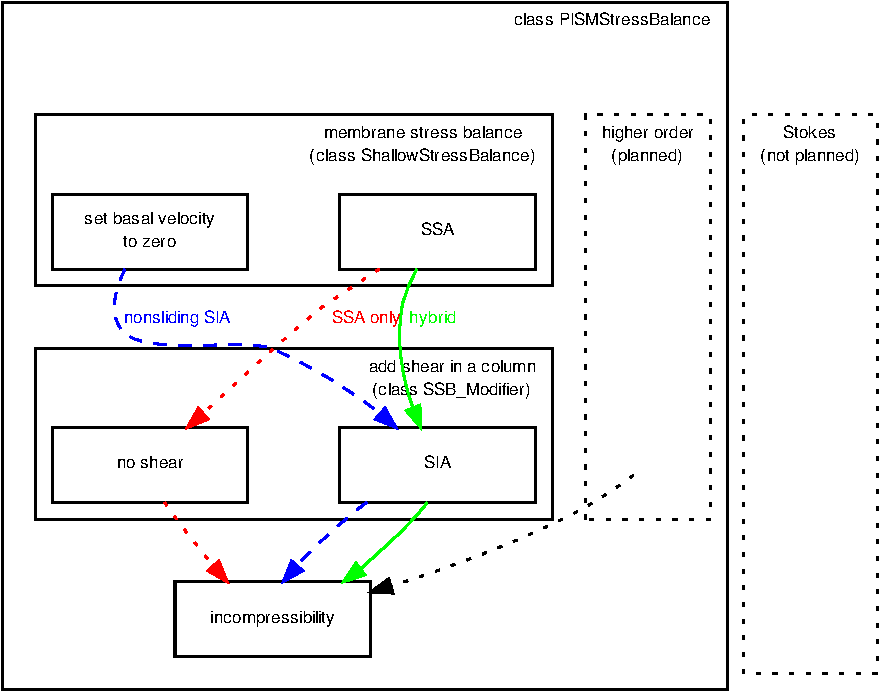
\includegraphics[width=6in]{stressbalance}
  \caption{The SIA-only, SSA-only, and SIA+SSA hybrid models represent different ``routes'' through stress balance PISM components.  In each case the inputs are ice geometry and boundary stresses, and the final output is a three-dimensional velocity field within the ice.}
  \label{fig:stressbalance}
\end{figure}

It may also be helpful to view the implemented stress balances as PISM software components (C++ classes).  Figure \ref{fig:stressbalance} shows the sequences of actions taken by the SIA-only, SSA-only, and SIA+SSA hybrid model components.  In each case a membrane stress solution is generated first, then a distribution of vertical shear in the column of ice is generated second, and finally a use of incompressibility computes the vertical component of the velocity.  The nonsliding SIA-only model has a trivialized membrane stress solution.  The SSA-only model has a trivialized computation of vertical shear.


\subsection{Evolutionary versus diagnostic modeling} \label{subsect:basicmodes}\index{PISM!evolution run}\index{PISM!diagnostic run}    The main goal of a numerical ice sheet model like PISM is to be a dynamical system which evolves as similarly as possible to the modeled ice sheet.  Such a goal assumes one has the ``right'' climate inputs and parameter choices at each time step.  It also assumes one has the ``right'' initial conditions, such as an adequate description of the present state of the ice sheet, but this assumption is rarely satisfied.  Instead a variety of heuristics must be used to minimally-initialize an ice sheet model.  For options associated to establishing mathematical initial conditions when first starting PISM, see section \ref{sec:initboot}.

Inside PISM are evolution-in-time partial differential equations which are solved by taking small time steps.  ``Small'' may vary from thousandths to tens of model years, in practice, depending primarily on grid resolution, but also on modeled ice geometry and flow speed.  Time steps are chosen adaptively in PISM, according to the stability criteria of the combined numerical methods \cite{BBssasliding,BBL}.

However, especially for ice streams and shelves, non-time-stepping ``diagnostic'' solution of the stress balance partial differential equations might be the desired computation, and PISM can also produce such ``diagnostic'' velocity fields.  Such computations necessarily assume that the ice geometry, viscosity, and boundary stresses are known.  Because of the slowness of the ice, in the sense that inertia can be neglected in the stress balance \cite{Fowler}, such computations can determine the ice velocity.

Sections \ref{sec:start} and \ref{sec:ross} give examples illustrating evolutionary and diagnostic modes of PISM, respectively.  The first describes time-stepping evolution models for the Greenland ice sheet, while the second describes a diagnostic SSA model for the Ross ice shelf.


\subsection{Climate inputs, and their interface with ice dynamics}
\label{sec:climate-inputs}  

\begin{figure}[ht]
  \centering
  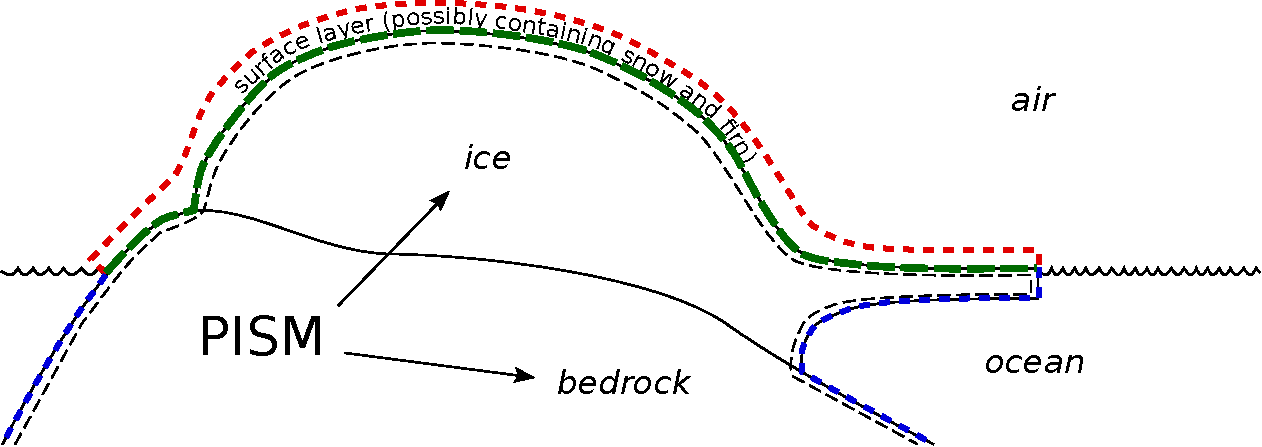
\includegraphics[width=6in]{figs/climate-cartoon.pdf}
  \caption{PISM's view of interfaces between an ice sheet and the outside world}
  \label{fig:climate-inputs}
\end{figure}

Because PISM's job is to approximate ice flow, its ``world view'' is centered around ice dynamics.  The discussion of boundary conditions in this Manual is thus ice-dynamics-centric.  On the other hand, there is no constraint on the nature of, or completeness of, climate models which could be coupled to PISM.  This section therefore explains a PISM organizing principle, namely that \emph{climate inputs affect ice dynamics by a well-defined interface}.

Almost no attempt is made here to describe the physics of the climate around ice sheets, so see \cite{massbalanceglossary} for terminology and \cite{Hock05} for a review of how surface melt can be modeled.  See the Climate Forcing Manual for much more information on PISM's climate-coupling-related options and on the particular fields which are shared between the ice dynamics core and the climate model.  Table \ref{tab:ice-dynamics-bc} lists fields which are needed as boundary conditions at the interfaces.

All PISM ice sheet models have some kind of interface (\textcolor{ForestGreen}{\textbf{green}} in Figure \ref{fig:climate-inputs}) to a subaerial surface processes layer containing snow, firn, and liquid (or refrozen) runoff.  The surface layer is assumed to cover the whole surface of the ice, and all grounded areas that the ice might occupy, including ablation areas and ice-free land.  We also always have an interface (\textcolor{blue}{\textbf{blue}}) to the ocean, but this interface is inactive if there is no floating ice.

\begin{table}[ht]
  \centering
 \begin{tabular}{p{0.45\linewidth}p{0.5\linewidth}}
    \toprule
    \textbf{Boundary surface} & \textbf{Fields (conditions)} \\
    \midrule
    upper surface of the surface processes layer (\textcolor{red}{\textbf{red}}) & \emph{optional}; typically: air temperature, precipitation \\
    top ice surface, but below firn (\textcolor{ForestGreen}{\textbf{green}}) & \emph{required}: boundary temperature (or enthalpy), mass flux (SMB) into the ice\\
    ice shelf basal surface (\textcolor{blue}{\textbf{blue}}) & \emph{required}: mass flux into the ocean, boundary temperature\\
    bottom surface of thermally-modeled bedrock layer (not shown) & \emph{required}: geothermal flux\\
   \bottomrule
  \end{tabular}
\caption{Boundary conditions required by PISM's ice dynamics core; see Figure \ref{fig:climate-inputs}.  The optional \textcolor{red}{\textbf{red}} interface is absent if PISM does not ``own'' the surface processes layer.}
\label{tab:ice-dynamics-bc}
\end{table}

The surface processes layer might be very simple.  It might either read the important fields from a file or otherwise transfer them from a separate (non-PISM) climate model.  If, however, the surface processes layer is ``owned'' by the PISM model then there is an additional interface (\textcolor{red}{\textbf{red}}) to the atmosphere above.  In no case does PISM ``own'' the atmosphere; if it has an interface to the atmosphere at all then it reads atmosphere fields from a file or otherwise transfers them from a climate model.

Regarding the base of the ice, the temperature of a layer of bedrock in contact with grounded ice is generally included in PISM's conservation of energy model; see subsections \ref{subsect:coords} and \ref{subsect:grid}.   Also, as described in section \ref{subsect:beddef}, PISM can apply an optional bed deformation component approximating the movement of the Earth's crust and upper mantle in response to changing ice load.  In these senses everything below the black dashed line in Figure \ref{fig:climate-inputs} is always ``owned'' by PISM.

The PISM ice dynamics core would like to get the required fields listed in Table
\ref{tab:ice-dynamics-bc} directly from observations or measurements, or directly from a GCM.  In many realistic modeling situations, however, PISM code must be used for all or part of the surface processes modeling necessary to provide the ice-dynamics core with the needed fields.  Due to differences in model resolutions and required down-scaling, this need for some PISM-based boundary-processes modelling may occur even in some cases where PISM is coupled to a GCM.  Thus, to be able to use the data that is available, a PISM run might use components that are responsible for modeling surface (snow) processes or sub-shelf/ocean interaction.  These components might be very minimal, merely turning data that we already have into data in the right units and with the right metadata.

\begin{figure}[ht]
  \centering
  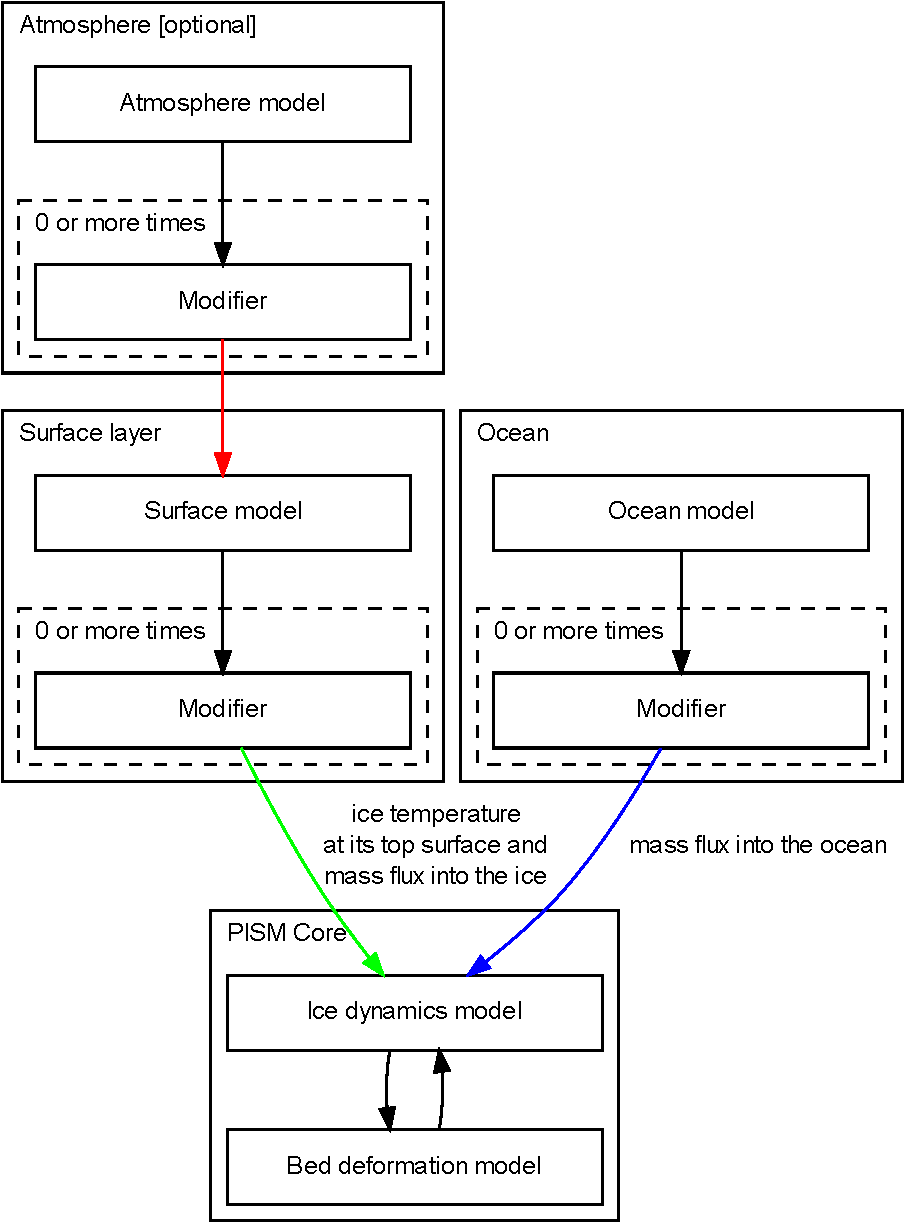
\includegraphics[width=4.0in]{figs/data-flow.pdf}
  \caption{PISM climate input data flow. Colored arrows correspond to interfaces in
    Figure \ref{fig:climate-inputs}.}
  \label{fig:climate-input-data-flow}
\end{figure}

Thus we have PISM's design: the ice-dynamics PISM core does not contain any parameterization or other model for boundary mass or energy fluxes into or out of the ice.  These boundary parameterizations and models are present in the PISM source code, however, as instances of \emph{pism::Component} classes.  This simplifies customizing and debugging PISM's climate inputs, and it promotes code reuse.  It isolates the code that needs to be changed to couple PISM to different climate models.

The classes \mbox{\emph{pism::SurfaceModel}}, \mbox{\emph{pism::AtmosphereModel}}, and \mbox{\emph{pism::OceanModel}} are all derived from \mbox{\emph{pism::Component}}.  Corresponding to the \textcolor{red}{\textbf{red}} dashed line in Figure~\ref{fig:climate-inputs}, a \mbox{\emph{pism::AtmosphereModel}} might not even be present in some PISM configurations.  While they are required, \emph{pism::SurfaceModel} and \emph{pism::OceanModel} may contain (hide) anything from nearly-trivial parameterizations of ice surface temperatures and mass fluxes to a GCM of great complexity.  

The ``modifiers'' in Figure \ref{fig:climate-input-data-flow} adjust the
climate model inputs.  Modifiers can be chained together so that multiple modifications
are made to the outputs of the original component.  For example,
ice-core-derived air temperature offsets, used to model the space-time
distribution of paleo-climatic surface temperature, is an example of an
implemented modifier.  Please see the Climate Forcing Manual for
a list of climate components and modifiers included in PISM source code and other details.
Users wishing to customize PISM's climate inputs and/or couple PISM to a climate
model should additionally see the \emph{PISM Source Browser} at \url{\PISMBROWSERURL}
and the documentation therein.

Figure~\ref{fig:climate-input-data-flow} illustrates the data flow needed
by the ice dynamics core.  The data flow in the other direction, i.e.~needed by the
model to which PISM is coupled, depends on particular modeling choices, but
great flexibility is allowed.

Why describe all this structure here?  On the one hand, some users may be interested
in coupling PISM to other models.  On the other hand, the PISM authors do not
claim expertise in modeling atmosphere, ocean, or even snow processes.  This
separation has a definite code-reliability purpose.  PISM users
are ultimately responsible for providing the climate inputs they intend.


\clearpage\newpage

\section{Initialization and bootstrapping}
\label{sec:initboot}
\optsection{Initialization}\optseealso{Input and output}

There are three ways to start PISM:\begin{itemize}
\item option \fileopt{i} reads a previously-saved ``complete'' PISM model state in a NetCDF file, or
\item option \fileopt{i} \intextoption{bootstrap} reads an ``incomplete'' NetCDF file and uses heuristics to fill in needed fields, or
\item one of the executables \texttt{pisms} or \texttt{pismv} is used to initialize simplified-geometry experiments or verification tests from formulas in the source code, and thus no input file is required.
\end{itemize}
One of the first two choices is required when using the executable \texttt{pismr}.  Modeling usually starts with the \texttt{-i input.nc -bootstrap} option because real ice sheet observations are never complete initial conditions.  Runs with multiple stages often use the \texttt{-i} option after the first stage.

\subsection{Initialization from a saved model state}  ``Initialization''\index{initialization!from saved model state} has the specific, simple meaning in PISM that option ``\texttt{-i}'' was used.  If a previous PISM run has saved a NetCDF file using ``\texttt{-o}'' then that file will contain complete initial conditions for continuing the run.  The output file from the last run can be loaded with ``\texttt{-i}'': \index{executables!\texttt{pisms}}

\begin{verbatim}
$ pisms -eisII A -y 100 -o foo.nc
$ pisms -eisII A -i foo.nc -y 100 -o bar.nc
\end{verbatim}
\smallskip

As noted verification tests (section \ref{sec:verif}) and simplified-geometry experiments (section \ref{sec:simp}) do not need input files at all because they initialize from formulas in the source code.  They can, however, be continued from saved model states using \texttt{-i}.  Specifying the simplified geometry experiment or verification test \emph{is}, however, necessary if the run is to continue with the climate inputs for that experiment or test.  For example, based on the above \texttt{pisms} runs, it is valid to do
\begin{verbatim}
$ pismr -i foo.nc -y 100 -o bar.nc
\end{verbatim}
but the climate and other parameters use PISM default values, and thus are not (necessarily) the values specified in EISMINT II.

As a technical note about saved states, a PISM run with \texttt{-stress_balance ssa} also saves the last SSA velocities to the output file in variables \texttt{u_ssa} and \texttt{v_ssa}.  The presence of these velocities adds efficiency in restarting because an initial estimate speeds up the solution of the SSA stress balance equations.  If you want to use \texttt{-i} but also ignore these velocities then use option \intextoption{dontreadSSAvels}.

\subsubsection*{\texttt{-i} file format}
\label{sec:i-format}
PISM produces CF-1.5 compliant NetCDF\index{PISM!NetCDF file format}\index{NetCDF} files.  The easiest way to learn the output format \emph{and} the \texttt{-i} format is to do a simple run and then look at the metadata in the resulting file, like this:
\begin{verbatim}
$ pisms -eisII A -y 10 -o foo.nc
$ ncdump -h foo.nc | less
\end{verbatim}

Note that variables in the output file have a \texttt{pism_intent}\index{PISM!\texttt{pism_intent} attribute} attribute.  When \texttt{pism_intent} = \texttt{diagnostic}, the variable can be deleted from the file without affecting whether PISM can use it as a \texttt{-i} input file.  Variables with \texttt{pism_intent} = \texttt{model_state}, by contrast, must be present when using \texttt{-i}.

The automatically-produced \texttt{time} variable has a \texttt{units} attribute like \texttt{"seconds since 1-1-1"} because the CF metadata conventions require a reference date.  By default PISM ignores this reference date except when it is used in unit conversions based on a calendar (see below).


\subsection{Bootstrapping}
\label{sec:bootstrapping}
\optsection{Bootstrapping}
\optseealso{Grid}
\optseealso{Input and output}

``Bootstrapping''\index{bootstrapping}\index{initialization!by bootstrapping} in PISM means starting a modeling run with less than sufficient data, and letting essentially heuristic models fill in needed fields.  These heuristics are applied before the first time step is taken, so they are part of an initialization process.  Bootstrapping uses the option \intextoption{bootstrap}; see subsection \ref{subsect:runscript} for an example.

The need for an identified stage like ``bootstrapping'' comes from the fact that initial conditions for the evolution equations describing an ice sheet are not all observable.  As a principal example of this problem, these initial conditions include the temperature within the ice.  Glaciological observations, specifically remote-sensed observations which cover a large fraction or all of an ice sheet, never include this temperature field in practice.  Thus ice sheet modelling often does something like this to get ``reasonable'' initial fields within the ice:
\begin{enumerate}
\item start only with (potentially) observable quantities like surface elevation, ice thickness, ice surface temperature, surface mass balance, and geothermal flux,
\item ``bootstrap'' as defined here, using heuristics to fill in temperatures at depth and to give a preliminary estimate of the basal sliding condition and the three-dimensional velocity field, and
\item \begin{enumerate}
      \item \emph{either} do a long run, often holding the current geometry and surface conditions steady, to evolve toward a steady state which has compatible temperature, stress, and velocity fields,
      \item \emph{or} do a long run using an additional (typically spatially-imprecise) historical record from an ice core or a sea bed core (or both), to apply forcing to the surface temperature or sea level (for instance), but with the same functional result of filling in temperature, stress, and velocity fields.
      \end{enumerate}
\end{enumerate}

When using \intextoption{bootstrap} you will need to specify both grid dimensions (using \texttt{-Mx}, \texttt{-My} and \texttt{-Mz}; see subsection \ref{subsect:grid}) and the height of the computational box for the ice with \texttt{-Lz} (subsection \ref{subsect:coords}).  The data read from the file can determine the horizontal extent of the model, if options \texttt{-Lx}, \texttt{-Ly} are not set.  The additional required specification of vertical extent by \texttt{-Lz} is reasonably natural because typical data used in ``bootstrapping'' are two-dimensional.  Using \texttt{-bootstrap} without specifying all four options \texttt{-Mx}, \texttt{-My}, \texttt{-Mz}, \texttt{-Lz} is an error.

If \texttt{-Lx} and \texttt{-Ly} specify horizontal grid dimensions smaller than in the bootstrapping file, PISM will cut out the center portion of the domain.  Alternatively, options \intextoption{x_range} and \intextoption{y_range} each take a list of two numbers, a list of minimum and maximum $x$ and $y$ coordinates, respectively (in meters), which makes it possible to select a subset that is not centered in the bootstrapping file's grid.

For the key issue of what heuristic is used to determine the temperatures at depth, there are two methods.  The default method uses ice thickness, surface temperature, surface mass balance, and geothermal flux.  The temperature is set to the solution of a steady one-dimensional differential equation in which conduction and vertical advection are in balance, and the vertical velocity linearly-interpolates between the surface mass balance rate at the top and zero at the bottom.  The non-default method, set with option \intextoption{boot_temperature_heuristic quartic_guess}, was the default in older PISM versions (\texttt{stable0.5} and earlier); it does not use the surface mass balance and instead makes a more-heuristic estimate of the vertical temperature profile based only on the ice thickness, surface temperature, and geothermal flux.

\subsubsection*{\texttt{-bootstrap} file format}
\label{sec:bootstrapping-format}

Allowed formats for a bootstrapping file are relatively simple to describe. 
\begin{enumerate}
\item NetCDF variables should have the \texttt{units} containing a
  UDUNITS-2-compatible string. If this attribute is missing, PISM will assume
  that a field uses MKS units.\footnote{PISM uses a library called UDUNITS-2\index{PISM!uses UDUNITS when reading NetCDF files}\index{UDUNITS-2} to convert data present in an input file to MKS.   This means that having ice thickness in feet or temperature in Fahrenheit \emph{is} allowed.}
\item NetCDF coordinate variables should have \texttt{standard_name} or
  \texttt{axis} attributes. These are used to
  determine which \emph{spatial} dimension a NetCDF dimension corresponds to;
  for example see \texttt{ncdump -h} output from a file produced by PISM.  The
  \texttt{x} and \texttt{y} dimensions need not be called ``\texttt{x}''
  and ``\texttt{y}''.
\item Coordinate variables have to be strictly-increasing.
\item Three-dimensional variables will be ignored in bootstrapping.
\item The \texttt{standard_name} attribute is used, when available, to identify a variable, so
  variable names need not match corresponding variables in a
  PISM output file.  See \url{\PISMBROWSERURL} for a list of CF standard
  names used in PISM.  Specifically, the bed elevation (topography) is read by
  \texttt{standard_name} = \texttt{bedrock_altitude} and the ice thickness by
  \texttt{standard_name} = \texttt{land_ice_thickness}.
\item Any two-dimensional variable except bed topography and ice thickness may
  be missing. For missing variables some heuristic will be applied. See
  table \ref{tab:modelhierarchy} for a sketch of the data necessary for
  bootstrapping; see \texttt{src/base/iMbootstrap.cc} for all further details.
\item Surface elevation is ignored if present. Users with surface elevation and
  bed elevation data should compute the ice thickness variable, put it in the
  bootstrapping file, and set its \texttt{standard_name} to \texttt{land_ice_thickness}.
\end{enumerate}


\clearpage\newpage

\section{Modeling choices: Grid and time}
\label{sec:modeling-computational}

\subsection{Computational box} \label{subsect:coords}
\optsection{Computational box}
\optseealso{Grid}

PISM does all simulations in a computational box\index{PISM!computational box} which is rectangular in the PISM coordinates.  The coordinate system has horizontal coordinates $x,y$ and a vertical coordinate $z$.  The $z$ coordinate is measured positive upward from the base of the ice.  The vector of gravity is in the negative $z$ direction.  The surface $z=0$ is the base of the ice, however, and thus is usually not horizontal in the sense of being parallel to the geoid.   The surface $z=0$ is the base of the ice both when the ice is grounded and when the ice is floating.

When the ice is grounded, the true physical vertical coordinate $z'$, namely the coordinate measure relative to a reference geoid, is given by $z'=z+b(x,y)$ where $b(x,y)$ is the bed topography.  The surface $z'=h(x,y)$ is the surface of the ice.  In the grounded case the equation $h(x,y)=H(x,y)+b(x,y)$ always applies if $H(x,y)$ is the thickness of the ice.

In the floating case, the physical vertical coordinate is $z'=z-(\rho_i/\rho_s) H(x,y)$ where $\rho_i$ is the density of ice and $\rho_s$ the density of sea water.  Again $z=0$ is the base of the ice, which is the surface $z' = -(\rho_i/\rho_s) H(x,y)$.  The surface of the ice is $h(x,y) = (1-\rho_i/\rho_s) H(x,y)$.  The \emph{flotation criterion} $-(\rho_i/\rho_s) H(x,y) > b(x,y)$ applies.

The computational box can extend downward into the bedrock.  As $z=0$ is the base of the ice, the bedrock corresponds to negative $z$ values regardless of its true (i.e.~$z'$) elevation.

The extent of the computational box, along with its bedrock extension downward, is determined by four numbers \texttt{Lx}, \texttt{Ly}, \texttt{Lz}, and \texttt{Lbz} (see Figure \ref{fig:rectilinearbox} and Table \ref{tab:compbox}).  The first two of these are half-widths and have units of kilometers when set by options or displayed.

\begin{figure}[ht]
\centering
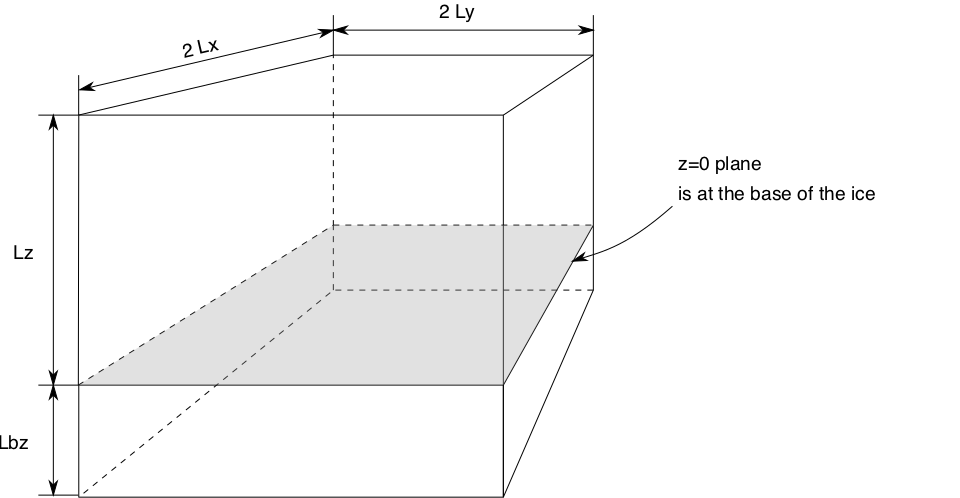
\includegraphics[width=4.0in,keepaspectratio=true]{rectilinearbox}
\caption{PISM's computational box.}
\label{fig:rectilinearbox}
\end{figure}

\begin{table}
  \centering
  \begin{tabular}{llp{0.7\linewidth}}
    \toprule
    \textbf{Option} & \textbf{Meaning}
    \\\midrule
    \txtopt{Lx}{(km)} & Half-width of the computational domain (in the $x$-direction) \\
    \txtopt{Ly}{(km)} & Half-width of the computational domain (in the $y$-direction) \\
    \txtopt{Lz}{(meters)} & Height of the computational domain; must exceed maximum ice thickness \\
    \txtopt{Lbz}{(meters)} & Depth of the computational domain in the bedrock thermal layer
    \\\bottomrule
  \end{tabular}
  \caption{Options defining the extent of PISM's computational box.}
  \label{tab:compbox}
\end{table}


\subsection{Spatial grid}
\label{subsect:grid}
\optsection{Grid!space}

The PISM grid\index{PISM!grid} covering the computational box is equally spaced in horizontal ($x$ and $y$) directions.  Vertical spacing in the ice is quadratic by default but optionally equal spacing can be chosen; choose with options \txtopt{z_spacing}{[\texttt{quadratic}, \texttt{equal}]} at bootstrapping.  The grid read from a ``\texttt{-i}'' input file is used as is.  The bedrock thermal layer model always uses equal vertical spacing.

The grid is described by four numbers, namely the number of grid points \texttt{Mx} in the $x$ direction, the number \texttt{My} in the $y$ direction, the number \texttt{Mz} in the $z$ direction within the ice, and the number \texttt{Mbz} in the $z$ direction within the bedrock thermal layer.  These are specified by options \intextoption{Mx}, \intextoption{My}, \intextoption{Mz}, and \intextoption{Mbz}, respectively. The defaults are 61, 61, 31, and 1, respectively.  Note that \texttt{Mx}, \texttt{My}, \texttt{Mz}, and \texttt{Mbz} all indicate the number of grid \emph{points} so the number of grid \emph{spaces} are one less, thus 60, 60, 30, and 0 in the default case.

The lowest grid point in a column of ice, at $z=0$, coincides with the highest grid point in the bedrock, so \texttt{Mbz} must always be at least one.  Choosing \texttt{Mbz}$>1$ is required to use the bedrock thermal model.  When a thermal bedrock layer is used, the distance \texttt{Lbz} is controlled by the \texttt{-Lbz} option.  Note that \texttt{Mbz} is unrelated to the bed deformation model (glacial isostasy model); see section \ref{subsect:beddef}.

In the quadratically-spaced case the spacing near the ice/bedrock interface is about four times finer than it would be with equal spacing for the same value of \texttt{Mz}, while the spacing near the top of the computational box is correspondingly coarser.  For a detailed description of the spacing of the grid, see the documentation on \texttt{IceGrid::compute_vertical_levels()} in the PISM class browser.

The user should specify the grid when using \texttt{-bootstrap} or when initializing a verification test (section \ref{sec:verif}) or a simplified-geometry experiment (section \ref{sec:simp}).  If one initializes PISM from a saved model state using \texttt{-i} then the input file determines all grid parameters.  For instance, the command

\begin{verbatim}
$  pismr -i foo.nc -y 100
\end{verbatim}

\noindent should work fine if \texttt{foo.nc} is a PISM output file.  Because \texttt{-i} input files take precedence over options,

\begin{verbatim}
$  pismr -i foo.nc -Mz 201 -y 100
\end{verbatim}

\noindent will give a warning that ``\texttt{PISM WARNING: ignoring command-line option '-Mz'}''.


\subsubsection{Parallel domain distribution}
\label{sec:domain-dstribution}
\optsection{Grid!domain distribution}

When running PISM in parallel with \texttt{mpiexec -n N}, the horizontal grid is distributed across $N$ processes\footnote{In most cases one process corresponds to one ``core'' of your computer.}.  PISM divides the grid into $N_x$ parts in the $x$ direction and $N_y$ parts in the $y$ direction.  By default this is done automatically, with the goal that $N_x\times N_y = N$ and $N_x$ is as close to $N_y$ as possible.  Note that $N$ should, therefore, be a composite (not prime) number.

Users seeking to override this default can specify $N_x$ and $N_y$ using the \intextoption{Nx} and \intextoption{Ny} command-line options.

Once $N_x$ and $N_y$ are computed, PISM computes sizes of sub-domains $M_{x,i}$ so that $\sum_{i=1}^{N_x}M_{x,i} = \mathrm{Mx}$ and $M_{x,i} - \left\lfloor \mathrm{Mx} / N_x \right\rfloor < 1$. To specify strip widths $M_{x,i}$ and $M_{y,i}$, use command-line options \intextoption{procs_x} and \intextoption{procs_y}. Each option takes a comma-separated list of numbers as its argument. For example,
\begin{verbatim}
$ mpiexec -n 3 pisms -Mx 101 -My 101 -Nx 1 -Ny 3 -procs_x 101 -procs_y 20,61,20
\end{verbatim}
%$ - match dollar signs to make emacs happy
splits a $101 \times 101$ grid into 3 strips along the $x$ axis.

To see the parallel domain decomposition from a completed run, see the \texttt{rank} variable in the output file, e.g.~using \texttt{-o_size big}.  The same \texttt{rank} variable is available as a spatial diagnostic field (subsection \ref{sec:saving-spat-vari}).


\subsection{Model time}
\label{sec:time}
\optsection{Grid!time}

Table \ref{tab:timeoptions} gives the command-line options which control PISM time.  If option \texttt{-ys} is absent then the start year is read from the input file (if present) or it defaults to zero.  The default value for the end year is the start year plus the given (\texttt{-y}) run length.  If both \texttt{-ys} and \texttt{-ye} are used then the run length is set to the difference.  Using all three of \texttt{-ys}, \texttt{-y} and \texttt{-ys} is not allowed; this generates an error message.

\begin{table}
\begin{tabular}{lp{0.8\linewidth}}\\
\toprule
\textbf{Option} & \textbf{Meaning}\\
\midrule
\txtopt{y}{(years)} & Number of model years to run.\\
\txtopt{ys}{(years)} & Model year at which to start the run.  Also resets the model time, ignoring any time in the input file.\\
\txtopt{ye}{(years)} & Model year at which to end the run.\\
\bottomrule
\end{tabular}
\caption{Command-line options controlling PISM time.}
\label{tab:timeoptions}
\end{table}


\subsection{Calendars}
\label{sec:calendars}
\index{Time!calendars}

Most of PISM, and its ice dynamics core in particular, only needs to know the length of the current time-step.  Internally PISM stores time in ``seconds since a specified moment'' and thus PISM generally does not use or need a calendar.\footnote{Note seconds are part of SI units.}  We refer to PISM internal time as \emph{model time}.

One can select a calendar for more precise control of the model time, however.  A ``calendar'' is a concept that is part of the \href{http://cf-pcmdi.llnl.gov/documents/cf-conventions/1.6/cf-conventions.html}{CF Metadata Conventions}.  Choosing a calendar is appropriate for runs for specific temporal periods like ``the 18th-century'' or ``1989--2010''.  The calendar is generally needed because  specific knowledge of lengths of months and years is required to use climate data properly or to facilitate model validation.

PISM uses \href{http://meteora.ucsd.edu/~pierce/calcalcs/index.html}{CalCalcs} by David~W.~Pierce to perform calendric computations.  This lets us support all the calendars \href{http://cf-pcmdi.llnl.gov/documents/cf-conventions/1.6/cf-conventions.html#calendar}{defined} by the CF Metadata Conventions document except for the \texttt{366_day} (\texttt{all_leap}) calendar.

Time units in PISM's output files always contain a reference date because it is required by the CF metadata conventions.

By default PISM does not use a calendar. This is appropriate for runs that do not require precise application of forcing data or reporting on particular dates (paleo-climate runs, for example).  In this mode PISM ignores the reference date in time unit specifications (such as ``\texttt{days since 1969-7-20}''), though the value set using \config{reference_date} configuration parameter is saved in (is passed forward into) output files.

\begin{table}
  \centering
  \begin{tabular}{lp{0.7\linewidth}}
    \texttt{gregorian} or \texttt{standard} & Mixed Gregorian/Julian calendar used today.\\
    \texttt{proleptic_gregorian} & Gregorian calendar extended to dates before 1582-10-15.\\
    \texttt{noleap} or \texttt{365_day} & Calendar with fixed-length 365-day years\\
    \texttt{360_day} & Calendar with fixed-length 360-day years divided into 30-day months\\
    \texttt{julian} & Julian calendar \\
    \texttt{none} & no calendar\\
  \end{tabular}
  \caption{Calendars supported by PISM. Please see \href{http://meteora.ucsd.edu/~pierce/calcalcs/calendars.html}{CalCalcs documentation} for details.}
  \label{tab:calendars}
\end{table}

Selecting a calendar using the \config{calendar} configuration parameter or the \intextoption{calendar} command-line option enables calendar-based time management; see Table \ref{tab:calendars}.  The implications of selecting a calendar are:
\begin{itemize}
\item PISM uses the \texttt{units} attribute of coordinate variables
  \emph{literally} (including the reference date) in unit conversions. Please
  make sure that the \variable{time} variable in all forcing files has the
  units attribute such as ``\texttt{days since 2012-1-1}''. PISM will stop with
  an error message if a time variable does not have a reference date in its
  unit specification.
\item It is important to use units that are a fixed multiple of ``seconds'',
  such as ``\texttt{minutes since 1989-1-1}'' or ``\texttt{days since
    1999-12-31}'' and avoid ``months'' and ``years''. (PISM uses UDUNITS-2 to
  convert units, and in UDUNITS one month is always interpreted as
  $\frac{1}{12}\cdot 365.242198781$ days.) Please see the 
  \href{http://cf-pcmdi.llnl.gov/documents/cf-conventions/1.6/cf-conventions.html#time-coordinate}{CF
    Conventions} document for details.
\item PISM uses dates in standard output:
\begin{verbatim}
...
   time interval (length)   [2012-01-01, 2021-12-31]  (10.000 years)
...
S 2012-05-26:  0.00011    0.6306   0.00000000           0.00000
$v$Eh m (dt=0.10000)
S 2012-07-01:  0.00014    0.6306   0.00000000           0.00000
\end{verbatim}
\end{itemize}

Just like in the no-calendar mode, run length, run start and run end
times are specified using \intextoption{y}, \intextoption{ys} and
\intextoption{ye} command-line options, respectively. Arguments of
these options are interpreted in a slightly different manner, though:
\begin{itemize}
\item the run length option \texttt{-y} takes an \emph{integer}
  argument, interpreted as the number of \emph{calendar} years
\item options \texttt{-ys} and \texttt{-ye} take \emph{dates} as arguments.
\end{itemize}

For example, either of the following commands sets up a run covering the 21$^{st}$ century:
\begin{verbatim}
$ pismr -calendar gregorian -ys 2001-1-1 -y 100 ...
$ pismr -calendar standard -ys 2001-1-1 -ye 2101-1-1 ...
\end{verbatim}
(These option combinations are equivalent.)

It is also possible to run PISM for the duration of the available forcing data using the \fileopt{time_file} option.  The command
\begin{verbatim}
$ pismr -calendar gregorian -time_file forcing.nc
\end{verbatim}
%$ - match dollar signs to make emacs happy
will extract the reference date and run length from \texttt{forcing.nc}, respecting time bounds.

When a non-trivial calendar is selected, spatial and scalar time-series can be saved daily, monthly or yearly using these calendric computations. See sections~\ref{sec:saving-time-series} and~\ref{sec:saving-spat-vari}.

\subsubsection{Re-starting an interrupted run using \texttt{-time_file}}
\label{sec:time-file-restart}

If a run using \texttt{-time_file} gets interrupted but manages to save a backup, re-starting with \texttt{-time_file} will attempt to re-do the entire run because options \texttt{-y}, \texttt{-ys}, and \texttt{-ye} are ignored:
\begin{verbatim}
# This run gets killed but leaves backup.nc:
$ pismr -i input.nc -time_file time.nc -o output.nc
# This WILL NOT start from the time saved in backup.nc
# and continue until the end time in time.nc
$ pismr -i backup.nc -time_file time.nc -o output.nc
\end{verbatim}
In this case we want to set the start time of the run from \texttt{backup.nc}, but use the end time from \texttt{time.nc}. To achieve this, use the option \intextoption{time_file_continue_run}.
\begin{verbatim}
# This run gets killed but leaves backup.nc:
$ pismr -i input.nc -time_file time.nc -o output.nc
# This WILL continue until the end time in time.nc, starting from backup.nc
$ pismr -i backup.nc -time_file time.nc -o output.nc -time_file_continue_run
\end{verbatim}

\subsection{Diagnostic computations}
\label{sec:diagnostic-computations}

A ``diagnostic'' computation can be defined as one where the internal state does not evolve.  The internal state of PISM is the set of variables read by ``\texttt{-i}''.  You can ask PISM to do a diagnostic computation by setting the run duration to a small number such as $0.001$ years (about $9$ hours). The duration to use depends on the modeling setup, but should be smaller than the maximum time-step allowed by PISM's stability criteria. Such short runs can also be used to look at additional fields corresponding to the current model state.

As an example, consider these two runs:
\begin{verbatim}
pisms -y 6000 -o foo.nc
pismr -i foo.nc -y 0.001 -o bar.nc -o_size big
\end{verbatim}

\noindent The result of the second (short) run is a NetCDF file \texttt{bar.nc} which contains the full three-dimensional velocity field in the scalar NetCDF variables \texttt{uvel}, \texttt{vvel}, and \texttt{wvel}, as well as many other variables.  The file \texttt{foo.nc} does not contain many of these fields because it was written with the default output size of \texttt{medium}.  The ``\texttt{-y 0.001}'' run has diagnostically ``filled-in'' all the fields which PISM can model at a time step, but the run duration was chosen so as to avoid significant model state evolution during the run.

This diagnostic mode is often associated to the modeling of ice shelves and ice streams.  Subsection \ref{sec:ross} describes using a short ``diagnostic'' run to model the Ross ice shelf \cite{MacAyealetal}.  Verification tests I and J, section \ref{sec:verif}, are diagnostic calculations using the SSA.

The NetCDF model state saved by PISM at the end of an \emph{evolution} run (i.e.~with ``\texttt{-y }$Y$'' for $Y>0$) does not, under the default \texttt{-o_size medium} output size, contain the three-dimensional velocity field.  Instead, it contains just a few more variables than those which are needed to restart the run with \texttt{-i}.  One can  force PISM to save all the supported diagnostic quantities at the end of a time-stepping run using the option \texttt{-o_size big}.  Or one can go back and do a ``\texttt{-y small_number}'' diagnostic run using \texttt{-o_size big}.


\subsection{Disabling PISM components}
\label{sec:turning-off}
\optsection{Disabling PISM components}

Certain major model components, unlike more peripheral ones like bed deformation or calving, are ``on'' by default.  They do not need to be turned on explicitly.  For example, the SIA computation is so common that it would be a hassle to require an option to turn it on every time you need it.

But sometimes one wants to disable particular components, during model spin-up, for example.  PISM has the following ``off'' switches:
\begin{itemize}
\item \intextoption{no_mass} disables the mass-continuity (conservation of mass) step
\item \intextoption{energy none} disables the conservation of energy computation
\item \intextoption{energy cold} makes PISM use temperature instead of enthalpy in the energy conservation code
\item \intextoption{stress_balance none} disables the stress balance computation (useful for testing surface mass balance inputs)
\end{itemize}


\subsection{Dealing with more difficult modeling choices}
\label{subsec:hard-choices}\optsection{Dealing with more difficult modeling choices}

Most uses of an ice sheet model depend on careful modeling choices in situations where there are considerable uncertainties \emph{and} the model results depend strongly on those choices.  There may be, at the present state of knowledge, \emph{no clear default values} that PISM can provide.  Furthermore, the available PISM options and sub-models are known to \emph{not} be sufficient for all users.  Thus there are modelling situations for which we know the user may have to do a great deal more hard work than just choose among PISM runtime options.

Here are example cases where users have worked hard:
\begin{itemize}
\item User made use of available data in order to choose parameters for existing PISM models.  These parameters then override PISM defaults.
\begin{center} % our UAF current situation with Greenland
\fbox{ \begin{minipage}[t]{5.0in}
\emph{Example}.  Use regional atmosphere model output to identify PDD parameters suitable for modeling surface mass balance on a particular ice sheet.  Then supply these parameters to PISM by a \texttt{-config\_override} file.
\end{minipage} }
\end{center}
\item User wrote code, including code which modified current PISM internals, either to add additional processes or to ``correct'' PISM default process models.
\begin{center} % the ocean coupler-related Potsdam marine ice sheet mods
\fbox{ \begin{minipage}[t]{5.0in}
\emph{Example}.  Add a new sub-ice-shelf melt model by modifying C++ code in the \texttt{src/coupler/} directory.
\end{minipage} }
\end{center}
\item User simplified the model in use, instead of the default which was more elaborate.
\begin{center} % Nick's -yield_stress constant choice
\fbox{ \begin{minipage}[t]{5.0in}
\emph{Example}.  Instead of using the PISM default mechanism connecting basal melt rate and basal strength, bypass this mechanism by generating a map of yield stress \texttt{tauc} directly and supplying it as input.
\end{minipage} }
\end{center}
\end{itemize}


%%% Local Variables: 
%%% mode: latex
%%% TeX-master: "manual"
%%% End: 

% LocalWords:  


\clearpage\newpage

\section{Modeling choices:  Ice dynamics and thermodynamics}
\label{sec:modeling-dynamics}

\subsection{Choosing the stress balance}
\label{subsect:stressbalance}
\optsection{Stress balance}

The basic stress balance used for all grounded ice in PISM is the non-sliding, thermomechanically-coupled SIA \cite{BBL}.  For the vast majority of most ice sheets, as measured by area or volume, this is an appropriate model, which is an $O(\eps^2)$ approximation to the Stokes model if $\eps$ is the depth-to-length ratio of the ice sheet \cite{Fowler}.

The shallow shelf approximation (SSA)\index{SSA (shallow shelf approximation)} stress balance applies to floating ice.  See the Ross ice shelf example in section \ref{sec:ross} for an example in which the SSA is only applied to floating ice.

The SSA is also used in PISM to describe the sliding of grounded ice and the formation of ice streams \cite{BBssasliding}.  Specifically for the SSA with ``plastic'' (Coulomb friction) basal resistance, the locations of ice streams are determined as part of a free boundary problem of Schoof \cite{SchoofStream}, a model for emergent ice streams within a ice sheet and ice shelf system.  This model explains ice streams through a combination of plastic till failure and SSA stress balance.

This SSA description of ice streams is, however, also the preferred ``sliding law'' for the SIA \cite{BBssasliding,Winkelmannetal2011}.  The SSA should be combined with the SIA, in this way, in preference to classical SIA sliding laws which make ice basal velocity a local function of the basal value of the driving stress.\index{SIA (shallow ice approximation)!sliding laws}.  The resulting combination of SIA and SSA is a ``hybrid'' approximation of the Stokes model \cite{Winkelmannetal2011}.  Option \texttt{-stress_balance ssa+sia} turns on this ``hybrid'' model.  In this use of the SSA as a sliding law, floating ice is also subject to the SSA.

Of course there is more to the use of a stress balance than just turning it on!  At all grounded points a yield stress, or a pseudo-yield-stress in the case of power law sliding (subsection \ref{subsect:basestrength}), is computed from the amount of stored basal water and from a (generally) spatially-varying till strength.  The amount of stored basal water is modeled by the subglacial hydrology mode choice (subsection \ref{subsect:subhydro}) based on the basal melt rate which is, primarily, thermodynamically-determined (subsection \ref{subsect:basestrength}).

Table \ref{tab:stress-balance-choice} describes the basic choice of stress balance.  If the SSA stress balance is used, a choice of two solvers is available, namely \texttt{-ssa_method fd} (default) or \texttt{-ssa_method fem}.  See Table \ref{tab:ssa-usage}, which describes additional controls on the numerical solution of the stress balance equations.  If option \texttt{-ssa_method fd} is chosen then several more controls on numerics are available; see Table \ref{tab:ssafd-controls}.  If the ice sheet being modeled has any floating ice then the user is advised to read section \ref{sec:pism-pik} on modeling marine ice sheets.

\begin{table}[ht]
\centering
\small
\begin{tabular}{p{0.4\linewidth}p{0.5\linewidth}}
\toprule
\textbf{Option} & \textbf{Semantics}\\ \midrule
  \intextoption{stress_balance none} & Turn off ice flow completely.\\
  \intextoption{stress_balance sia} \mbox{(default)} & Grounded ice flows by the non-sliding SIA.  Floating ice essentially doesn't flow, so this model is not recommended for marine ice sheets. \\
  \intextoption{stress_balance ssa} & Use the SSA model exclusively. Horizontal ice velocity is constant throughout ice columns.\\
  \intextoption{stress_balance \mbox{prescribed_sliding}} & Use the constant-in-time prescribed sliding velocity field read from a file set using \fileopt{prescribed_sliding_file}, variables \texttt{ubar} and \texttt{vbar}. Horizontal ice velocity is constant throughout ice columns. \\
  \intextoption{stress_balance ssa+sia} & The recommended sliding law, which gives the SIA+SSA hybrid stress balance.  Combines SSA-computed velocity, using pseudo-plastic till, with SIA-computed velocity according to the combination in \cite{Winkelmannetal2011}; similar to \cite{BBssasliding}.  Floating ice uses SSA only. \\
  \intextoption{stress_balance \mbox{prescribed_sliding+sia}} & Use the constant-in-time prescribed sliding velocity in combination with the non-sliding SIA.\\
\bottomrule
\end{tabular}
\normalsize
\caption{The basic choice of stress balance.}
\label{tab:stress-balance-choice} 
\end{table}


\begin{table}[ht]
  \centering
  \begin{tabular}{p{0.25\linewidth}p{0.7\linewidth}}
     \toprule
     \textbf{Option (default)} & \textbf{Description}\\\midrule
     \intextoption{ssa_method} [\texttt{fd}$\big|$\texttt{fem}] & Both finite difference (\texttt{fd}; the default) and finite element (\texttt{fem}) versions of the SSA numerical solver are implemented in PISM.  The \texttt{fd} solver is the only one which allows PIK options (section \ref{sec:pism-pik}).  \texttt{fd} uses Picard iteration \cite{BBssasliding}, while \texttt{fem} uses a Newton method.  The \texttt{fem} solver has surface velocity inversion capability \cite{Habermannetal2013}.  \\
     \intextoption{ssa_eps} ($10^{13}$) & The numerical schemes for the SSA compute an effective viscosity $\nu$ which depends on strain rates and ice hardness (thus temperature).  The minimum value of the effective viscosity times the thickness (i.e.~$\nu H$) largely determines the difficulty of solving the numerical SSA.  This constant is added to keep $\nu H$ bounded away from zero: $\nu H \to \nu H + \text{\texttt{ssa_eps}}$.  Units of \texttt{ssa_eps} are $\text{Pa}\,\text{m}\,\text{s}$.  Set to zero to turn off this lower bound. \\
     \intextoption{ssa_view_nuh}  & View the product $\nu H$ for your simulation as a runtime viewer (section \ref{sec:diagnostic-viewers}).  In a typical Greenland run we see a wide range of values for $\nu H$ from $\sim 10^{14}$ to $\sim 10^{20}$ $\text{Pa}\,\text{m}\,\text{s}$. \\
\bottomrule
\end{tabular}
\caption{Choice of, and controls on, the numerical SSA stress balance.}
\label{tab:ssa-usage}
\end{table}

\begin{table}[ht]
  \centering
  \bigskip
  \begin{tabular}{p{0.25\linewidth}p{0.7\linewidth}}
     \toprule
     \textbf{Option (default)} & \textbf{Description}\\\midrule
%FIXME: this should be "ssafd_picard_maxi"?
     \intextoption{ssa_maxi} (300) & Set the maximum allowed number of Picard (nonlinear) iterations in solving the shallow shelf approximation.\\
%FIXME: this should be "ssafd_picard_rtol"?
     \intextoption{ssa_rtol} ($10^{-4}$) & The Picard iteration computes a vertically-averaged effective viscosity which is used to solve the equations for horizontal velocity.  Then the new velocities are used to recompute an effective viscosity, and so on.  This option sets the relative change tolerance for the effective viscosity.  The Picard iteration stops when successive values $\nu^{(k)}$ of the vertically-averaged effective viscosity satisfy
      $$\|(\nu^{(k)} - \nu^{(k-1)}) H\|_1 \le Z \|\nu^{(k)} H\|_1$$
where $Z=$ \texttt{ssa_rtol}. \\
    \intextoption{ssafd_ksp_rtol} ($10^{-5}$) & Set the relative change tolerance for the iteration inside the Krylov linear solver used at each Picard iteration. \\
\bottomrule
\end{tabular}
\caption{Controls on the numerical iteration of the \texttt{-ssa_method fd} solver.}
\label{tab:ssafd-controls}
\end{table}

\clearpage


\subsection{Ice rheology}
\label{sec:rheology}
\optsection{Ice rheology}

The ``rheology'' of a viscous fluid refers to the relation between the applied stress and the resulting deformation, the strain rate.  The models of ice rheology available in PISM are all isotropic \cite{Paterson}.   A rheology in this class is described by a ``flow law'', which is, in the most general case in PISM, a function $F(\sigma,T,\omega,P,d)$ in the ``constitutive relation'' form
\begin{equation}
D_{ij} = F(\sigma,T,\omega,P,d)\, \sigma_{ij}'.  \label{eq:constitutive}
\end{equation}
Here $D_{ij}$ is the strain rate tensor, $\sigma_{ij}'$ is the stress deviator tensor, $T$ is the ice temperature, $\omega$ is the liquid water fraction, $P$ is the pressure, $d$ is the grain size, and $\sigma^2 = \frac{1}{2} \|\sigma_{ij}'\|_F = \frac{1}{2} \sigma_{ij}' \sigma_{ij}'$ defines the second invariant $\sigma$ of the stress deviator tensor.

Form \eqref{eq:constitutive} of the flow law is used in the SIA, but the ``viscosity'' form of a flow law, found by inverting the constitutive relation \eqref{eq:constitutive}, is needed for ice shelf and ice stream (SSA) flow \cite{BBssasliding}:
\begin{equation}
\sigma_{ij}' = 2 \nu(D,T,\omega,P,d)\,D_{ij}  \label{eq:viscosityform}
\end{equation}
Here $\nu(D,T,\omega,P,d)$ is the ``effective viscosity'' and $D^2 = \frac{1}{2} D_{ij} D_{ij}$.

Most of the flow laws in PISM are of Glen-Nye single-power type.  For example,
\begin{equation}
F(\sigma,T) = A(T) \sigma^{n-1}  \label{eq:glen}
\end{equation}
is the common temperature-dependent Glen law \cite{PatersonBudd,BBL} (which has no dependence on liquid water fraction, pressure, or grain size).  If the ice softness $A(T)=A_0$ is constant then the law is isothermal, whereas if there is dependence on temperature then $A(T)$ is usually a generalization of ``Arrhenius'' form $A(T) = A \exp(-Q/(R T))$.

The more elaborate Goldsby-Kohlstedt law \cite{GoldsbyKohlstedt} is a function $F(\sigma,T,P,d)$, but in this case the function $F$ cannot be factored into a product of a function of $T,P,d$ and a single power of $\sigma$, as in form \eqref{eq:glen}.

There is only one choice for the flow law which takes full advantage of the enthalpy mode of PISM, which is the thermodynamical modeling (i.e.~conservation of energy) default.  Namely the Glen-Paterson-Budd-Lliboutry-Duval flow law \cite{AschwandenBuelerKhroulevBlatter,LliboutryDuval1985,PatersonBudd}, which is a function $F(\sigma,T,\omega,P)$.  This law is the only one in the literature where the ice softness depends on both the temperature and the liquid water fraction, so it parameterizes the (observed) softening of pressure-melting-temperature ice as its liquid fraction increases.  One can use this default polythermal law or one may choose among a number of ``cold ice'' laws listed in Table \ref{tab:flowlaw} which do not use the liquid water fraction.  

All flow law parameters can be changed using configuration parameters; see section \ref{sec:pism-defaults} and the implementation of flow laws in the \emph{Source Code Browser}.  Note that different flow laws have different numbers of parameters, but all have at least two parameters (e.g.~$A_0$ and $n$ in \texttt{isothermal_glen}).  One can create a new, and reasonably arbitrarily, scalar function $F$ by modifying source code; see source files \texttt{flowlaws.hh}, \texttt{flowlaws.cc} in \texttt{src/base/rheology/}.  To assist such modifications, note that Table \ref{tab:flowlaw} below also lists the C++ classes declared in \texttt{flowlaw.hh}.

\subsubsection*{Choosing the flow laws for SIA and SSA stress balances}  Command-line options \intextoption{sia_flow_law} and \intextoption{ssa_flow_law} choose which flow law is used by the SIA and SSA stress balances, respectively.  Allowed arguments are listed in Tables \ref{tab:flowlaw} and \ref{tab:flowlawgk} below.  Viscosity form \eqref{eq:viscosityform} is not known for the Goldsby-Kohlstedt law \cite{GoldsbyKohlstedt}, so option ``\texttt{-ssa_flow_law gk}'' is an error.

\begin{table}[ht]
\centering
\index{rheology}\index{flow law}
\small
\begin{tabular}{p{0.16\linewidth}p{0.2\linewidth}p{0.58\linewidth}}\toprule
\textbf{Name} & C++ Class & \textbf{Comments and References} \\ \midrule
\texttt{gpbld} &\texttt{GPBLD}  & Glen-Paterson-Budd-Lliboutry-Duval law \cite{LliboutryDuval1985}, the enthalpy-based default in PISM \cite{AschwandenBuelerKhroulevBlatter}.  Extends the Paterson-Budd law (below) to positive liquid water fraction.  If $A_{c}(T)$ is from Paterson-Budd then this law returns $A(T,\omega) = A_{c}(T) (1 + C \omega)$, where $\omega$ is the liquid water fraction, $C$ is a configuration parameter \texttt{gpbld_water_frac_coeff} [default $C=181.25$], and $\omega$ is capped at level \texttt{gpbld_water_frac_observed_limit}.  \\  \midrule
\texttt{pb} &\texttt{PatersonBudd}  & Paterson-Budd law, the cold-mode default.  Fixed Glen exponent $n=3$.  Has a split ``Arrhenius'' term $A(T) = A \exp(-Q/RT^*)$ where \mbox{$A = 3.615 \times 10^{-13}\, \text{s}^{-1}\, \text{Pa}^{-3}$}, \mbox{$Q = 6.0 \times 10^4\, \text{J}\, \text{mol}^{-1}$} if $T^* < 263$ K and
 \mbox{$A = 1.733 \times 10^{3}\, \text{s}^{-1}\, \text{Pa}^{-3}$}, \mbox{$Q = 13.9 \times 10^4\, \text{J}\, \text{mol}^{-1}$} if $T^* > 263$ K; here $T^*$ is pressure-adjusted temperature \cite{PatersonBudd}. \\
\texttt{arr} &  \texttt{PatersonBuddCold} & \emph{Cold} part of Paterson-Budd.  Regardless of temperature, the $A$ and $Q$ values for $T^*<263$ K in  the Paterson-Budd law apply.  This is the flow law used in the thermomechanically-coupled exact solutions run by \texttt{pismv -test F} and \texttt{pismv -test G} \cite{BBL,BB}. \\
\texttt{arrwarm} & \texttt{PatersonBuddWarm} & \emph{Warm} part of Paterson-Budd.  Regardless of temperature, the $A$ and $Q$ values for $T^*>263$ K in Paterson-Budd apply.\\
\texttt{hooke} & \texttt{Hooke} & Hooke law with \mbox{$A(T) = A \exp(-Q/(RT^*) + 3C (T_r - T^*)^\kappa)$.}  Fixed Glen exponent $n=3$ and constants as in \cite{Hooke,PayneBaldwin}.\\
\texttt{isothermal_glen} &  \texttt{IsothermalGlen} & The isothermal Glen flow law.  Here $F(\sigma) = A_0 \sigma^{n-1}$ with inverse $\nu(D) = \frac{1}{2} B_0 D^{(1-n)/(2n)}$ where $A_0$ is the ice softness and $B_0=A_0^{-1/n}$ is the ice hardness. \\
\bottomrule
\normalsize	
\end{tabular}
\caption{Single-power flow laws.  Choose the ice rheology using \texttt{-sia_flow_law} and \texttt{-ssa_flow_law} and one of the above names.  Flow law choices other than \texttt{gpbld} do not use the liquid water fraction $\omega$ but only the temperature $T$.}
\label{tab:flowlaw}
\end{table}

\begin{table}[ht]
\centering
\index{rheology}\index{flow law}
\small
\begin{tabular}{p{0.1\linewidth}p{0.2\linewidth}p{0.55\linewidth}}\toprule
\textbf{Name} & C++ Class & \textbf{Comments and References} \\ \midrule
\texttt{gk} & \texttt{GoldsbyKohlstedt} & This law has a combination of exponents from $n=1.8$ to $n=4$ \cite{GoldsbyKohlstedt}.  It can only be used by the SIA stress balance.  Because it has more than one power, option \texttt{-sia_n} has no effect, though \texttt{-sia_e} works as expected.  This law does not use the liquid water fraction, but only the temperature. \\
\bottomrule
\normalsize	
\end{tabular}
\caption{The Goldsby-Kohlstedt flow law. Use option \texttt{-sia_flow_law gk}.}
\label{tab:flowlawgk}
\end{table}


\subsubsection*{Choose enhancement factor and exponent}  An enhancement factor can be added to any flow law through a runtime option.  Single-power laws also permit control of the flow law exponent through a runtime option.

Options \intextoption{sia_e} and \intextoption{ssa_e} set flow enhancement factors for the SIA and SSA respectively.  Option \texttt{-sia_e} sets ``$e$'' in ``$D_{ij} = e\, F(\sigma,T,\omega,P,d)\, \sigma_{ij}',$'' in equation \eqref{eq:constitutive}.  Option \texttt{-ssa_e} sets ``$e$'' in the viscosity form so that ``$\sigma_{ij}'  = e^{-1/n}\, 2\, \nu(D,T,\omega,P,d)\, D_{ij}.$''

Options \intextoption{sia_n} and \intextoption{ssa_n} set the exponent when a single-power flow law is used (see Table \ref{tab:flowlaw}).  Simply changing to a different value from the default $n=3$ is not recommended without a corresponding change to the enhancement factor, however.  This is because the coefficient and the power are non-trivially linked when a power law is fit to experimental data \cite{CuffeyPaterson,PatersonBudd}.

Here is a possible approach to adjusting both the enhancement factor and the exponent.  Suppose $\sigma_0$ is preferred as a scale (reference) for the driving stress that appears in both SIA and SSA models.  Typically this is on the order of one bar or $10^5$ Pa.  Suppose one wants the same amount of deformation $D_0$ at this reference driving stress as one changes from the old exponent $n_{old}$ to the new exponent $n_{new}$.  That is, suppose one wants both
  $$D_0 = E_{old}\, A\, \sigma_0^{n_{old}} \qquad \text{and} \qquad D_0 = E_{new}\, A\, \sigma_0^{n_{new}}$$
to be true with a new enhancement factor $E_{new}$.  Eliminating $D_0$ and solving for the new enhancement factor gives
\begin{equation}
E_{new} = E_{old}\, \sigma_0^{n_{old} - n_{new}}.  \label{eq:renewexponent}
\end{equation}
It follows, for example, that if one has a run with values
\begin{quote}
\texttt{-sia_e 3.0 -sia_n 3.0}
\end{quote}
then a new run with exponent $n=6.0$ and the same deformation at the reference driving stress of $10^5$ Pa will use
\begin{quote}
\texttt{-sia_e 3.0e-15 -sia_n 6.0}
\end{quote}
because $E_{new} = 3.0 \sigma_0^{3-6} = 3.0 \times (10^5)^{-3}$ from equation \eqref{eq:renewexponent}.

A corresponding formula applies to \texttt{-ssa_e} if the \texttt{-ssa_n} value changes.

\begin{table}[ht]
\centering
\bigskip
\index{flow law exponent}\index{enhancement factor}
\small
\begin{tabular}{p{0.18\linewidth}p{0.26\linewidth}p{0.5\linewidth}}\toprule
\textbf{Option (default)} & \textbf{Configuration parameter} & \textbf{Comments} \\ \midrule
\intextoption{sia_e} (1.0) & \texttt{sia_enhancement_factor} & Note \cite[see supplement]{AschwandenAdalgeirsdottirKhroulev} used $3.0$ for Greenland ice sheet simulations while \cite{Martinetal2011} used $4.5$ for simulations of the Antarctic ice sheet with PISM-PIK. \\
\intextoption{sia_n} (3.0) & \texttt{sia_Glen_exponent} & See text and eqn \eqref{eq:renewexponent} to also set \texttt{-sia_e} if \texttt{-sia_n} changes. \\
\intextoption{ssa_e} (1.0) & \texttt{ssa_enhancement_factor} & Note \cite{Martinetal2011} used $0.512$ for simulations of the Antarctic ice sheet with PISM-PIK. \\
\intextoption{ssa_n} (3.0) & \texttt{ssa_Glen_exponent} & See text and eqn \eqref{eq:renewexponent} to also set \texttt{-ssa_e} if \texttt{-ssa_n} changes. \\
\bottomrule
\normalsize	
\end{tabular}
\caption{For all flow laws, an enhancement factor can be added by a runtime option.  For the single-power flow laws in Table \ref{tab:flowlaw}, the (Glen) exponent can be controlled by a runtime option.}
\label{tab:enhancementandexponent}
\end{table}

\clearpage


\subsection{Surface gradient method}
\label{subsect:gradient}
\optsection{Driving stress computation}

PISM computes surface gradients to determine the ``driving stress''
	$$(\tau_{d,x},\tau_{d,y}) = - \rho g H \grad h,$$
where $H$ is the ice thickness, and $h = H+b$ is the ice surface elevation.  The driving stress enters into both the SIA and SSA stress balances, but in the former the driving stress is needed on a staggered grid, while in the latter the driving stress is needed on the regular grid.

Surface gradients are computed by finite differences in several slightly-different ways.  There are options for choosing which method to use, but to the best of our knowledge there is no theoretical advice on the best, most robust mechanism.  There are three \intextoption{gradient} methods in PISM:

\noindent\texttt{-gradient mahaffy}\quad  This most ``standard'' way computes the surface slope onto the staggered grid for the SIA \cite{Mahaffy}.  It makes $O(\Delta x^2,\Delta y^2)$ errors.  For computations of driving stress on the regular grid, centered differencing is used instead.

\noindent\texttt{-gradient haseloff}\quad  This is the default method.  It only differs from \texttt{mahaffy} at ice-margin locations, where it alters the formula for the slope in cases where an adjacent ice-free bedrock surface elevation is above the ice elevation.

\noindent\texttt{-gradient eta}\quad  In this method we first transform the thickness $H$ by $\eta = H^{(2n+2)/n}$ and then differentiate the sum of the thickness and the bed using centered differences:
	$$\grad h = \grad H + \grad b = \frac{n}{(2n+2)} \eta^{(-n-2)/(2n+2)} \nabla \eta + \nabla b.$$
Here $b$ is the bed elevation and $h$ is the surface elevation.  This transformation sometimes has the benefits that the surface values of the horizontal velocity and vertical velocity, and the driving stress, are better behaved near the margin.  See \cite{BLKCB} for technical explanation of this transformation and compare \cite{SaitoMargin}.  The actual finite difference schemes applied to compute the surface slope are similar to option \texttt{mahaffy}.


\subsection{Modeling conservation of energy} \label{subsect:energy}
\optsection{Energy conservation}

In normal use PISM solves the conservation of energy problem within the ice, the thin subglacial layer, and a layer of thermal bedrock.  For the ice and the subglacial layer it uses an enthalpy-based scheme \cite{AschwandenBuelerKhroulevBlatter} which allows the energy to be conserved even when the temperature is at the pressure-melting point.

Ice at the melting point is called ``temperate'' ice.  Part of the thermal energy of temperate ice is in the latent heat of the liquid water stored between the crystals of the temperate ice.  Part of the thermal energy of the whole glacier is in the latent heat of the liquid water under the glacier.  The enthalpy scheme correctly models these storehouses of thermal energy, and thus it allows polythermal and fully-temperate glaciers to be modeled \cite{AschwandenBlatter}.

The state of the full conservation of energy model includes the 3D \texttt{enthalpy} variable plus the 2D \texttt{bwat} and \texttt{tillwat} subglacial hydrology state variables (subsection \ref{subsect:subhydro}), all of which are seen in output files.  The important basal melt rate computation involves all of these energy state variables, because the basal melt rate (\texttt{bmelt} in output files) comes from conserving energy across the ice-bedrock layer \cite{AschwandenBuelerKhroulevBlatter}.  Fields \texttt{temp}, \texttt{liqfrac}, and \texttt{temp_pa} seen in output files are all actually diagnostic outputs because all of these can be recovered from the enthalpy and the ice geometry.

Because this part of PISM is just a conservation law, there is little need for the user to worry about controlling it.  If desired, however, conservation of energy can be turned off entirely with \intextoption{energy none}.  The default enthalpy-based conservation of energy model (i.e.~\texttt{-energy enthalpy}) can be replaced by the temperature-based (i.e.~``cold ice'') method used in \cite{BBssasliding} and verified in \cite{BBL} by setting option \intextoption{energy cold}.

The thermal bedrock layer model is turned off by setting \texttt{-Mbz 1} (i.e.~zero spaces) while it is turned on by choosing a depth and number of points, as in \texttt{-Lbz 1000 -Mbz 21}, for example, which gives a layer depth of 1000 m and grid spaces of 50 m (= 1000/20).  The input geothermal flux (\texttt{bheatflx} in output files) is applied at the bottom of the bedrock thermal layer if such a layer is present and otherwise it is applied at the base of the ice.


\subsection{Computing ice age} \label{subsect:age}
\optsection{Computing ice age}

By default, PISM does not compute the age of the ice\index{PISM!modeling the age of the ice} because it does not directly impact ice flow when using the default flow laws.  It is very easy to turn on.  Just set \intextoption{age}.  A 3D variable \texttt{age} will appear in output files.  It is read at input if \texttt{-age} is set and otherwise it is ignored even if present in the input file.  If \texttt{-age} is set and the variable \texttt{age} is absent in the input file then the initial age is set to zero.


%%% Local Variables: 
%%% mode: latex
%%% TeX-master: "manual"
%%% End: 

% LocalWords:  


\clearpage\newpage
\section{Modeling choices:  The subglacier}
\label{sec:modeling-subglacier}

\subsection{Controlling basal strength}  \label{subsect:basestrength}
\optsection{Basal strength and sliding}

When using option \intextoption{stress_balance ssa+sia}, the SIA+SSA hybrid stress balance, a model for basal resistance is required.  This model for basal resistance is based, at least conceptually, on the hypothesis that the ice sheet is underlain by a layer of till \cite{Clarke05}.  The user can control the parts of this model:\begin{itemize}
\item the so-called sliding law, typically a power law, which relates the ice base (sliding) velocity to the basal shear stress, and which has a coefficient which is or has the units of a yield stress,
\item the model relating the effective pressure on the till layer to the yield stress of that layer, and
\item the model for relating the amount of water stored in the till to the effective pressure on the till.
\end{itemize}
This subsection explains the relevant options.

The primary example of \texttt{-stress_balance ssa+sia} usage is in section \ref{sec:start} of this Manual, but the option is also used in sections \ref{subsect:MISMIP}, \ref{subsect:MISMIP3d}, \ref{sec:storglaciaren}, and \ref{sec:jako}.

In PISM the key coefficient in the sliding is always denoted as yield stress $\tau_c$, which is \texttt{tauc} in PISM output files.  This parameter represents the strength of the aggregate material at the base of an ice sheet, a poorly-observed mixture of pressurized liquid water, ice, granular till, and bedrock bumps.  The yield stress concept also extends to the power law form, and thus most standard sliding laws can be chosen by user options (below).  One reason that the yield stress is a useful parameter is that it can be compared, when looking at PISM output files, to the driving stress (\texttt{taud_mag} in PISM output files).  Specifically, where $\text{\tt tauc} < \text{\tt taud_mag}$ you are likely to see sliding if option \texttt{-stress_balance ssa+sia} is used.

A historical note on modeling basal sliding is in order.  Sliding can be added directly to a SIA stress balance model by making the sliding velocity a local function of the basal value of the driving stress.  Such an SIA sliding mechanism appears in ISMIP-HEINO \cite{Calovetal2009HEINOfinal} and in EISMINT II experiment H \cite{EISMINT00}, among other places.  This kind of sliding is \emph{not} recommended, as it does not make sense to regard the driving stress as the local generator of flow if the bed is not holding all of that stress \cite{BBssasliding,Fowler01}.  Within PISM, for historical reasons, there is an implementation of SIA-based sliding only for verification test E; see section \ref{sec:verif}.  PISM does \emph{not} support this SIA-based sliding mode in other contexts.

\subsubsection*{Choosing the sliding law}  In PISM the sliding law can be chosen to be a purely-plastic (Coulomb) model, namely,
\begin{equation}
   |\tau_b| \le \tau_c \quad \text{and} \quad \tau_b = \tau_c \frac{\mathbf{u}}{|\mathbf{u}|} \quad\text{if and only if}\quad |\mathbf{u}| > 0,
\label{eq:plastic}
\end{equation}
which says that the (vector) basal shear stress $\tau_b$ is at most the yield stress $\tau_c$, and only when the shear stress reaches the yield value can there be sliding.  Alternatively, the sliding law can be chosen to be a power law,
\begin{equation}
\tau_b = \tau_c \frac{\mathbf{u}}{u_{\text{threshold}}^q |\mathbf{u}|^{1-q}}.
\label{eq:pseudoplastic}
\end{equation}
Condition \eqref{eq:plastic} is studied in \cite{SchoofStream} and \cite{SchoofTill} in particular.  Power laws for sliding are common across the glaciological literature (e.g.~see \cite{CuffeyPaterson,GreveBlatter2009}), but we explain here the specific form of equation \eqref{eq:pseudoplastic}, which allows the coefficient $\tau_c$ to have units of stress regardless of the power $q$.

In both of the above equations \eqref{eq:plastic} and \eqref{eq:pseudoplastic} we call $\tau_c$ the \emph{yield stress}.  We call the power law \eqref{eq:pseudoplastic} a ``pseudo-plastic'' law with power $q$ and threshold velocity $u_{\text{threshold}}$.  Note that at the threshold velocity the basal shear stress $\tau_b$ has exact magnitude $\tau_c$.  In equation \eqref{eq:pseudoplastic}, $q$ is the power controlled by \texttt{-pseudo_plastic_q}, and the threshold velocity $u_{\text{threshold}}$ is controlled by \texttt{-pseudo_plastic_uthreshold}.  The plastic model \eqref{eq:plastic} is the $q=0$ case of \eqref{eq:pseudoplastic}.

See Table \ref{tab:sliding-power-law} for options controlling the choice of sliding law. The purely plastic case is the default; just use \texttt{-stress_balance ssa} \texttt{-stress_balance ssa+sia} to turn it on.

\begin{quote}
  \textbf{WARNING!} Options \texttt{-pseudo_plastic_q} and \texttt{-pseudo_plastic_uthreshold} have no effect if \texttt{-pseudo_plastic} is not set.
\end{quote}

In both equations \eqref{eq:plastic} and \eqref{eq:pseudoplastic}, $\tau_c$ corresponds to the variable \texttt{tauc} in PISM output files.

\begin{table}
  \centering
 \begin{tabular}{lp{0.6\linewidth}}
    \\\toprule
    \textbf{Option} & \textbf{Description}
    \\\midrule
    \intextoption{pseudo_plastic} & Enables the pseudo-plastic power law model.  If this is not set the sliding law is purely-plastic, so \texttt{pseudo_plastic_q} and \texttt{pseudo_plastic_uthreshold} are inactive. \\
    \txtopt{plastic_reg}{(m/a)} & Set the value of $\eps$ regularization of the plastic law, in the formula $\tau_b = \tau_c \mathbf{u}/\sqrt{|\mathbf{u}|^2 + \eps^2}$.  The default is $0.01$ m/a.  This parameter is inactive if \texttt{-pseudo_plastic} is set. \\
    \intextoption{pseudo_plastic_q} & Set the exponent $q$ in \eqref{eq:pseudoplastic}.  The default is $0.25$. \\
    \txtopt{pseudo_plastic_uthreshold}{(m/a)} & Set $u_{\text{threshold}}$ in \eqref{eq:pseudoplastic}.  The default is $100$ m/a.\\ \bottomrule
  \end{tabular}
\caption{Sliding law command-line options}
\label{tab:sliding-power-law}
\end{table}

Equation \eqref{eq:pseudoplastic} is a very flexible power law form.  For example, the linear case is $q=1$, in which case if $\beta=\tau_c/u_{\text{threshold}}$ then the law is of the form
\begin{equation*}
  \tau_b = \beta \mathbf{u}  
\end{equation*}
(The ``$\beta$'' coefficient is also called $\beta^2$ in some sources \cite[for example]{MacAyeal}.)  If you want such a linear sliding law, and you have a value $\beta=$\texttt{beta} in $\text{Pa}\,\text{s}\,\text{m}^{-1}$, then use this option combination:
\begin{verbatim}
-pseudo_plastic -pseudo_plastic_q 1.0 -pseudo_plastic_uthreshold 3.1556926e7 \
  -yield_stress constant -tauc beta
\end{verbatim}
\noindent This sets $u_{\text{threshold}}$ to 1 $\text{m}\,\text{s}^{-1}$ but using units $\text{m}\,\text{a}^{-1}$.

More generally, it is common in the literature to see power-law sliding relations in the form
\begin{equation*}
  \tau_b = C |\mathbf{u}|^{m-1} \mathbf{u},
\end{equation*}
where $C$ is a constant, as for example in sections \ref{subsect:MISMIP} and \ref{subsect:MISMIP3d}.  In that case, use this option combination:
\begin{verbatim}
-pseudo_plastic -pseudo_plastic_q m -pseudo_plastic_uthreshold 3.1556926e7 \
  -yield_stress constant -tauc C
\end{verbatim}

\subsubsection*{Determining the yield stress}

Other than setting it to a constant in some special cases, the above discussion does not determine the yield stress $\tau_c$.  As shown in Table \ref{tab:yieldstress}, there are two schemes for determining $\tau_c$:
\begin{itemize}
\item \texttt{-yield_stress mohr_coulomb} (the default) determines the yields stress by models of a till material property (the till friction angle) and a model of the effective pressure on the saturated till.
\item \texttt{-yield_stress constant} requires the yield stress to be supplied as time-independent data, or set to a time- and space-independent constant by a run-time option, while
\end{itemize}

In particular, option combination \texttt{-yield_stress constant -tauc X} can be used to fix the yield stress to have value $\tau_c=$\texttt{X} at all grounded locations and all times if desired, but note this is not necessarily a good modelling choice.

In normal modelling cases, variations in yield stress are part of the explanation of the locations of ice streams \cite{SchoofStream}.  The default model \texttt{-yield_stress mohr_coulomb} determines these variations in time and space.  The value of $\tau_c$ is determined in part by a subglacial hydrology model, including the modeled till-pore water amount \texttt{tillwat} (subsection \ref{subsect:subhydro}), which then determines the effective pressure $N_{til}$ (see below).  The value of $\tau_c$ is also determined in part by a material property field $\phi=$\texttt{tillphi}, the ``till friction angle''.  These quantities are related by the Mohr-Coulomb criterion \cite{CuffeyPaterson}:
\begin{equation}
   \tau_c = c_{0} + (\tan\phi)\,N_{til}.  \label{eq:mohrcoulomb}
\end{equation}
Here $c_0$ is called the ``till cohesion'', whose default value in PISM is zero \cite[formula (2.4)]{SchoofStream} but which can be set by option \intextoption{till_c_0}.

\begin{table}
  \centering
 \begin{tabular}{lp{0.6\linewidth}}
    \\\toprule
    \textbf{Option} & \textbf{Description}
    \\\midrule
    \intextoption{yield_stress mohr_coulomb} &   The default.  Use equation \eqref{eq:mohrcoulomb} to determine $\tau_c$.  Only effective if \texttt{-stress_balance ssa} or \texttt{-stress_balance ssa+sia} is also set. \\
    \intextoption{till_c_0} & Set the value of the till cohesion ($c_{0}$) in the plastic till model.  The value is a pressure, given in kPa.\\
   \intextoption{tauc_slippery_grounding_lines} & If set, replace normally-computed $\tau_c$ from Mohr-Coulomb relation, which uses the effective pressure from the modeled amount of water in the till, by the minimum value of $\tau_c$ from Mohr-Coulomb, i.e. by using the effective pressure corresponding to the maximum amount of till-stored water.  Does not alter the reported amount of till water, nor does this mechanism affect water conservation.\\
    \txtopt{plastic_phi}{(degrees)} & Use a constant till friction angle. The default is $30^{\circ}$.\\
    \txtopt{topg_to_phi}{\emph{list of 4 numbers}} & Compute $\phi$ using equation \eqref{eq:phipiecewise}.\\ \midrule
    \intextoption{yield_stress constant} &   Keep the current values of the till yield stress $\tau_c$.  That is, do not update them by the default model using the stored basal melt water.  Only effective if \texttt{-stress_balance ssa} or \texttt{-stress_balance ssa+sia} is also set. \\
    \intextoption{tauc} &   Directly set the till yield stress $\tau_c$, in units Pa, at all grounded locations and all times.  Only effective if used with \texttt{-yield_stress constant}, because otherwise $\tau_c$ is updated dynamically. \\ \bottomrule
  \end{tabular}
\caption{Command-line options controlling how yield stress is determined.}
\label{tab:yieldstress}
\end{table}

We find that an effective, though heuristic, way to determine $\phi=$\texttt{tillphi} is to make it a function of bed elevation \cite{AschwandenAdalgeirsdottirKhroulev,Martinetal2011,Winkelmannetal2011}.  This heuristic is motivated by hypothesis that basal material with a marine history should be weak \cite{HuybrechtsdeWolde}.  PISM has a mechanism setting $\phi$=\texttt{tillphi} to be a \emph{piecewise-linear} function of bed elevation.  The option is
\begin{verbatim}
-topg_to_phi phimin,phimax,bmin,bmax
\end{verbatim}
\newcommand{\phimin}{\phi_{\mathrm{min}}}
\newcommand{\phimax}{\phi_{\mathrm{max}}}
\newcommand{\bmin}{b_{\mathrm{min}}}
\newcommand{\bmax}{b_{\mathrm{max}}}
Thus the user supplies 4 parameters: $\phimin$, $\phimax$, $\bmin$, $\bmax$, where $b$ stands for the bed elevation.  To explain these, we define $M = (\phimax - \phimin) / (\bmax - \bmin)$.  Then
\begin{equation}
  \phi(x,y) =
  \begin{cases}
    \phimin, & b(x,y) \le \bmin, \\
    \phimin + (b(x,y) - \bmin) \,M, & \bmin < b(x,y) < \bmax, \\
    \phimax, & \bmax \le b(x,y).
  \end{cases}
  \label{eq:phipiecewise}
\end{equation}

It is worth noting that an earth deformation model (see section \ref{subsect:beddef}) changes $b(x,y)=$ used in \eqref{eq:phipiecewise}, so that a sequence of runs such as
\begin{verbatim}
pismr -i foo.nc -bed_def lc -stress_balance ssa+sia -topg_to_phi 10,30,-50,0 ... -o bar.nc
pismr -i bar.nc -bed_def lc -stress_balance ssa+sia -topg_to_phi 10,30,-50,0 ... -o baz.nc
\end{verbatim}
will use \emph{different} \texttt{tillphi} fields in the first and second runs.  PISM will print a warning during initialization of the second run:
\begin{verbatim}
* Initializing the default basal yield stress model...
  option -topg_to_phi seen; creating tillphi map from bed elev ...
PISM WARNING: -topg_to_phi computation will override the 'tillphi' field
              present in the input file 'bar.nc'!
\end{verbatim}
Omitting the \texttt{-topg_to_phi} option in the second run would make PISM continue with the same \texttt{tillphi} field which was set in the first run.

\subsection*{Determining the effective pressure}  When using the default option \texttt{-yield_stress mohr_coulomb}, the effective pressure on the till $N_{til}$ is determined by the modeled amount of water in the till.  Lower effective pressure means that more of the weight of the ice is carried by the pressurized water in the till and thus the ice can slide more easily.  That is, equation \eqref{eq:mohrcoulomb} sets the value of $\tau_c$ proportionately to $N_{til}$.  The amount of water in the till is, however, a nontrivial output of the hydrology (subsection \ref{subsect:subhydro}) and conservation-of-energy (section \ref{subsect:energy}) submodels in PISM.

Following \cite{Tulaczyketal2000}, based on laboratory experiments with till extracted from an ice stream in Antarctica, we use the following parameterization:
\begin{equation}
N_{til} = \delta P_o \, 10^{(e_0/C_c) \left(1 - (W_{til}/W_{til}^{max})\right)}  \label{eq:computeNtil}
\end{equation}
Here $P_o$ is the ice overburden pressure which is determined entirely by the ice thickness and density, $W_{til}=$ \texttt{tillwat} is the effective thickness of water in the till, $W_{til}^{max}$ is the maximum amount of water in the till (see subsection \ref{subsect:subhydro}), and the remaining parameters are set by options in Table \ref{tab:effective-pressure}.

\begin{table}
  \centering
 \begin{tabular}{lp{0.6\linewidth}}
    \\\toprule
    \textbf{Option} & \textbf{Description}
    \\\midrule
    \intextoption{till_reference_void_ratio} & $= e_0$ in \eqref{eq:computeNtil}, dimensionless, with default value 0.69 \cite{Tulaczyketal2000} \\
    \intextoption{till_compressibility_coefficient} & $= C_c$ in \eqref{eq:computeNtil}, dimensionless, with default value 0.12 \cite{Tulaczyketal2000} \\
    \intextoption{till_effective_fraction_overburden} & $= \delta$ in \eqref{eq:computeNtil}, dimensionless, with default value 0.01 \\ \bottomrule
  \end{tabular}
\caption{Command-line options controlling how till effective pressure $N_{til}$ in equation \eqref{eq:mohrcoulomb} is determined.}
\label{tab:effective-pressure}
\end{table}


\subsection{Subglacial hydrology}  \label{subsect:subhydro}
\optsection{Subglacial hydrology}

At the present time, two simple subglacial hydrology models are implemented and documented in PISM, namely \texttt{-hydrology null} and \texttt{-hydrology routing}.  The water source for both of these models is the energy conservation model which computes the basal melt rate \texttt{bmelt}, but see also option \texttt{-input_to_bed_file} (Table \ref{tab:hydrology}) for a mechanism to add water directly into the subglacial layer.  Some of the water put into the subglacial layer is stored locally in a layer of subglacial till by the hydrology model.  Depending on the hydrology model, some water is transported horizontally according to the gradient of the modeled hydraulic potential.

In both hydrology models a state variable \texttt{tillwat} records the effective thickness of the layer of liquid water in the till, and it is used to compute the effective pressure on the till (see the previous subsection).  The pressure of the transportable water \texttt{bwat} in the \texttt{routing} model does not relate directly to the effective pressure on the till.

\begin{table}
  \centering
 \begin{tabular}{lp{0.55\linewidth}}
    \\\toprule
    \textbf{Option} & \textbf{Description}
    \\\midrule
    \txtopt{hydrology_tillwat_max}{(m)} & Maximum effective thickness for water stored in till. \\
    \intextoption{hydrology_use_const_bmelt} & Replace the conservation-of-energy computed basal melt rate \texttt{bmelt} with a constant. \\
    \txtopt{hydrology_const_bmelt}{(m/a)} & If \texttt{-hydrology_use_const_bmelt} is set then use this to set the constant the rate (as water thickness per time). \\
    \fileopt{input_to_bed_file} & Specifies a NetCDF file which contains a time-dependent field \texttt{inputtobed} which has units of water thickness per time.  This rate is added to the \texttt{bmelt} rate. \\
% FIXME: leave undocumented?    \txtopt{input_to_bed_period}{(a)} & The period, in years, of \texttt{-input_to_bed_file} data. \\
% FIXME: leave undocumented?    \txtopt{input_to_bed_reference_year}{(a)} & The reference year for periodizing the \texttt{-input_to_bed_file} data. \\
    \bottomrule
  \end{tabular}
\caption{Subglacial hydrology command-line options for all hydrology models.}
\label{tab:hydrology}
\end{table}

\subsubsection*{The default model \texttt{-hydrology null} model}  In this model the water is \emph{not} conserved but it is stored locally in the till up to a specified amount; option \intextoption{hydrology_tillwat_max} sets that amount.  The water is not conserved in the sense that water above the \texttt{hydrology_tillwat_max} level is lost permanently.  This model is based on the ``undrained plastic bed'' concept of \cite{Tulaczyketal2000b}; see also \cite{BBssasliding}.  See Table \ref{tab:hydrologynull}.

This non-conserving \texttt{-hydrology null} model has been extensively used, in combination with the Mohr-Coulomb till described in subsection \ref{subsect:basestrength} above, in modelling ice streaming \cite[among others]{AschwandenAdalgeirsdottirKhroulev,BBssasliding}.  Many other combinations of the basal strength models and hydrology models in PISM have not been significantly tested.

\begin{table}
  \centering
 \begin{tabular}{lp{0.55\linewidth}}
    \\\toprule
    \textbf{Option} & \textbf{Description}
    \\\midrule
    \intextoption{hydrology null} & The default model.  Not mass conserving in the map-plane but much faster than \texttt{-hydrology routing}.  Based on ``undrained plastic bed'' model of \cite{Tulaczyketal2000b}. \\
    \small\txtopt{hydrology_tillwat_decay_rate_null}{(m/a)}\normalsize &  Applies only to \texttt{-hydrology null}.  Water stored in till accumulates at the computed basal melt rate minus this rate. \\    \bottomrule
  \end{tabular}
\caption{Subglacial hydrology command-line options for the \texttt{-hydrology null} model}
\label{tab:hydrologynull}
\end{table}

\subsubsection*{The mass-conserving \texttt{-hydrology routing} model}  In this model the water \emph{is} conserved in the map-plane.  Some water still gets put into the till, with the same maximum value \texttt{hydrology_tillwat_max}, but excess water is horizontally-transported.  An additional state variable \texttt{bwat} is used by \texttt{routing} for the effective thickness of the layer of transportable water.  This transportable water will flow in the direction of the negative of the gradient of the modeled hydraulic potential.  In the \texttt{routing} model this potential is calculated by assuming that the transportable subglacial water is at the overburden pressure \cite{Siegertetal2009}.  Ultimately the transportable water will reach the ice sheet grounding line or ice-free-land margin, at which point it will be lost.  The amount that is lost this way is reported to the user.

In this model there is an additional equation for transfer of water between the till (\texttt{tillwat}) and the transport system (\texttt{bwat}).  This transfer is governed by the differential equation
\begin{equation}  \label{eq:hydrologytransfer}
  \frac{\partial W_{til}}{\partial t} = \mu \left(\min\left\{\omega W,W_{til}^{max}\right\} - W_{til}\right)
\end{equation}
where $W_{til}=$ \texttt{tillwat} is the effective thickness of water in the till, $W=$ \texttt{bwat} is the effective thickness of water in the transport system, $\mu$ is the rate coefficient for the transfer, and $\omega$ is the proportion of $W$ that $W_{til}$ tends toward.  At all times $0 \le W_{til} \le W_{til}^{max}$ in this model.  Table \ref{tab:hydrologyrouting} describes how these parameters are set.

Several parameters are used in determining how water flows in the \texttt{routing} model.  Specifically, the horizontal subglacial water flux is determined by a generalized Darcy flux relation \cite{Clarke05,Schoofetal2012}
\begin{equation}  \label{eq:flux}
\bq = - k\, W^\alpha\, |\grad \psi|^{\beta-2} \grad \psi
\end{equation}
where $\bq$ is the lateral water flux, $W=$ \texttt{bwat} is the effective thickness of the layer of transportable water, $\psi$ is the hydraulic potential, and $k$, $\alpha$, $\beta$ are controllable parameters (Table \ref{tab:hydrologyrouting}).

In the \texttt{routing} model the hydraulic potential $\psi$ is determined by
\begin{equation}
\psi = P_o + \rho_w g (b + W)  \label{eq:hydraulicpotential}
\end{equation}
where $P_o=\rho_i g H$ is the ice overburden pressure, $g$ is gravity, $\rho_i$ is ice density, $\rho_w$ is fresh water density, $H$ is ice thickness, and $b$ is the bedrock elevation.

For most choices of the relevant parameters and most grid spacings, the \texttt{routing} model is at least two orders of magnitude more expensive computationally than is the \texttt{null} model.  This follows directly from the CFL-type time-step restriction on lateral flow of a fluid with velocity on the order of centimeters to meters per second (i.e.~the subglacial liquid water \texttt{bwat}) compared to the much slower velocity of the flowing ice above.  Therefore the user should start with short runs of order a few model years, use option \intextoption{report_mass_accounting} to see the time-stepping behavior at \texttt{stdout}, and use \texttt{daily} or even \texttt{hourly} reporting for scalar and spatially-distributed time-series to see hydrology model behavior.

\begin{table}
  \centering
 \begin{tabular}{lp{0.55\linewidth}}
    \\\toprule
    \textbf{Option} & \textbf{Description}
    \\\midrule
    \intextoption{hydrology routing} & Choose the mass-conserving horizontal transport model in which the pressure of transportable water is equal to overburden pressure. \\
    \txtopt{hydrology_hydraulic_conductivity}{$k$} &  $=k$ in formula \eqref{eq:flux}.  \\
    \txtopt{hydrology_null_strip}{(km)} &  In the boundary strip water is removed and this is reported.  This option simply specifies the width of this strip, which should typically be one or two grid cells. \\
    \txtopt{hydrology_gradient_power_in_flux}{$\beta$} &  $=\beta$ in formula \eqref{eq:flux}.  \\
    \txtopt{hydrology_thickness_power_in_flux}{$\alpha$} &  $=\alpha$ in formula \eqref{eq:flux}.  \\
    \intextoption{report_mass_accounting} &  At each major model time-step the amount of subglacial water lost to ice-free land, to the ocean, and into the ``null strip'' is reported. \\
    \txtopt{hydrology_tillwat_rate}{($\text{s}^{-1}$)} & $=\mu$ in equation \eqref{eq:hydrologytransfer}.  Rate coefficient for $W \leftrightarrow W_{til}$ transfer mechanism.  Defaults to $10^{-6} \text{s}^{-1}$. \\
    \intextoption{hydrology_tillwat_transfer_proportion} & $=\omega$ in equation \eqref{eq:hydrologytransfer}; dimensionless.  In $W \leftrightarrow W_{til}$ transfer mechanism, $W_{til}$ will be comparable to this multiple of $W$.  Defaults to $100$. \\    \bottomrule
  \end{tabular}
\caption{Command-line options specific to hydrology model \texttt{routing}.}
\label{tab:hydrologyrouting}
\end{table}

% FIXME  -hydrology distributed is not documented; controlled by options
% hydrology_roughness_scale, hydrology_cavitation_opening_coefficient,
% hydrology_creep_closure_coefficient, hydrology_regularizing_porosity
%    \intextoption{init_P_from_steady}  & Only applies to \texttt{-hydrology distributed}. \\


\subsection{Earth deformation models} \label{subsect:beddef} \index{earth deformation} \index{PISM!earth deformation models, using}
\optsection{Earth deformation models}

The option \txtopt{bed_def}{[\texttt{iso, lc}]} turns one of the two available bed deformation models.

The first model \texttt{-bed_def iso}, is instantaneous pointwise isostasy.  This model assumes that the bed at the starting time is in equilibrium with the load.  Then, as the ice geometry evolves, the bed elevation is equal to the starting bed elevation minus a multiple of the increase in ice thickness from the starting time: $b(t,x,y) = b(0,x,y) - f [H(t,x,y) - H(0,x,y)]$.  Here $f$ is the density of ice divided by the density of the mantle, so its value is determined by setting the values of \texttt{lithosphere_density} and \texttt{ice_density} in the configuration file; see subsection \ref{sec:pism-defaults}.  For an example and verification, see Test H in Verification section. 

The second model \texttt{-bed_def lc} is much more physical.  It is based on papers by Lingle and Clark \cite{LingleClark} and Bueler and others \cite{BLKfastearth}.  It generalizes and improves the most widely-used earth deformation model in ice sheet modeling, the flat earth Elastic Lithosphere Relaxing Asthenosphere (ELRA) model \cite{Greve2001}.  It imposes  essentially no computational burden because the Fast Fourier Transform is used to solve the linear differential equation \cite{BLKfastearth}.  When using this model in PISM, the rate of bed movement (uplift) is stored in the PISM output file and then is used to initialize the next part of the run.  In fact, if gridded ``observed'' uplift data is available, for instance from a combination of actual point observations and/or paleo ice load modeling, and if that uplift field is put in a NetCDF variable with standard name \texttt{tendency_of_bedrock_altitude} in the  \texttt{-boot_file} file, then this model will initialize so that it starts with the given uplift rate.

Here are minimal example runs to compare these models:
\begin{verbatim}
$ mpiexec -n 4 pisms -eisII A -y 8000 -o eisIIA_nobd.nc
$ mpiexec -n 4 pisms -eisII A -bed_def iso -y 8000 -o eisIIA_bdiso.nc
$ mpiexec -n 4 pisms -eisII A -bed_def lc -y 8000 -o eisIIA_bdlc.nc
\end{verbatim}
Compare the \texttt{topg}, \texttt{usurf}, and \texttt{dbdt} variables in the resulting output files.  See also the comparison done in \cite{BLKfastearth}.


\subsection{Parameterization of bed roughness in the SIA} \label{subsect:bedsmooth} \index{Parameterization of bed roughness}
\optsection{Parameterization of bed roughness}

Schoof \cite{Schoofbasaltopg2003} describes how to alter the SIA stress balance to model ice flow over bumpy bedrock topgraphy.  One computes the amount by which bumpy topography lowers the SIA diffusivity.  An internal quantity used in this method is a smoothed version of the bedrock topography.  As a practical matter for PISM, this theory improves the SIA's ability to handle bed roughness because it parameterizes the effects of ``higher-order'' stresses which act on the ice as it flows over bumps.  For additional technical description of PISM's implementation, see the \emph{Browser} page ``Using Schoof's (2003) parameterized bed roughness technique in PISM''.

This parameterization is ``on'' by default when using \texttt{pismr}.  There is only one associated option: \intextoption{bed_smoother_range} gives the half-width of the square smoothing domain in meters.  If zero is given, \texttt{-bed_smoother_range 0} then the mechanism is turned off.  The mechanism is on by default using executable \texttt{pismr}, with the half-width set to 5 km (\texttt{-bed_smoother_range 5.0e3}), giving Schoof's recommended smoothing size of 10 km \cite{Schoofbasaltopg2003}.

This mechanism is turned off by default in executables \texttt{pisms} and \texttt{pismv}.

Under the default setting \texttt{-o_size medium}, PISM writes fields \texttt{topgsmooth} and \texttt{schoofs_theta} from this mechanism.  The thickness relative to the smoothed bedrock elevation, namely \texttt{topgsmooth}, is the difference between the unsmoothed surface elevation and the smoothed bedrock elevation.  It is \emph{only used internally by this mechanism}, to compute a modified value of the diffusivity; the rest of PISM does not use this or any other smoothed bed.  The field \texttt{schoofs_theta} is a number $\theta$ between $0$ and $1$, with values significantly below zero indicating a reduction in diffusivity, essentially a drag coefficient, from bumpy bed.


%%% Local Variables: 
%%% mode: latex
%%% TeX-master: "manual"
%%% End: 

% LocalWords:  


\clearpage\newpage

\section{Modeling choices: Marine ice sheet modeling}
\label{sec:pism-pik}
\index{PISM!PISM-PIK}
\index{PISM!marine ice sheet modeling}
\optsection{Marine ice sheets}

PISM is often used to model whole ice sheets surrounded by ocean, with attached floating ice shelves, or smaller regions like outlet glaciers flowing into embayments and possibly generating floating tongues.  This section explains the geometry and stress balance mechanisms in PISM that apply to floating ice and especially at the vertical calving faces of floating ice.  The physics at calving fronts is very different from elsewhere on an ice sheet, because the flow is nothing like the lubrication flow addressed by the SIA, and nor is the physics like the sliding flow in the interior of an ice domain.  The needed physics at the calving front can be thought of as boundary condition modifications to the mass continuity equation and to the SSA stress balance equation.

References \cite{Albrechtetal2011,Levermannetal2012,Winkelmannetal2011} by authors in the research group of Prof.~Anders Levermann at the Potsdam Institute for Climate Impact Research (``PIK''), Germany, describe most of the mechanisms covered in this section.  These are all improvements to the grounded, SSA-as-a-sliding law model of \cite{BBssasliding}.  These improvements make PISM an effective Antarctic model, as demonstrated by \cite{Golledgeetal2013,Martinetal2011,Winkelmannetal2012}, among other publications.  These improvements had a separate existence as the ``PISM-PIK'' model from 2009--2010, but since PISM stable0.4 are part of PISM itself.  A summary of options to turn on most of these ``PIK'' mechanisms is in Table \ref{tab:pism-pik-part-grid}, while the PIK calving law called ``eigencalving'' \cite{Levermannetal2012} is included later in Table \ref{tab:calving}.  When in doubt, the PISM user should set option \intextoption{pik} to turn on all of mechanisms in Table \ref{tab:pism-pik-part-grid}, but the user must still choose a calving model.

\begin{table}[ht]
  \centering
 \begin{tabular}{lp{0.7\linewidth}}
    \\\toprule
    \textbf{Option} & \textbf{Description}
    \\\midrule
    \texttt{cfbc} & apply the stress boundary condition along the ice shelf calving front \cite{Winkelmannetal2011} \\
    \texttt{kill_icebergs} & identify and eliminate free-floating icebergs, which cause well-posedness problems for the SSA stress balance solver \cite{Winkelmannetal2011} \\
    \texttt{part_grid} & allow the ice shelf front to advance by a part of a grid cell, avoiding
	the development of unphysically-thinned ice shelves \cite{Albrechtetal2011} \\
    \texttt{part_redist} &  scheme which makes the -part_grid mechanism conserve mass  \cite{Albrechtetal2011} \\ 
    \midrule
    \intextoption{pik} & equivalent to option combination ``\texttt{-cfbc -kill_icebergs -part_grid -part_redist}'' \\
    \bottomrule
 \end{tabular}
\caption{Options which turn on PIK ice shelf front mechanisms (other than ``eigencalving'' \cite{Levermannetal2012}).}
\label{tab:pism-pik-part-grid}
\end{table}

\subsection{Flotation criterion, mask, and sea level}
\label{sec:floatmask}
\optsection{Marine ice sheets!Mask}

The most basic decision about marine ice sheet dynamics made internally by PISM is whether a ice-filled grid cell is floating.  That is, PISM applies the ``flotation criterion'' \cite{Winkelmannetal2011} at every time step and at every grid location to determine whether the ice is floating on the ocean or not.  The result is stored in the \texttt{mask} variable.  The \texttt{mask} variable has \texttt{pism_intent} = \texttt{diagnostic}, and thus it does \emph{not} need to be included in \texttt{-i} or \texttt{-boot_file} input files.

The possible values of the \texttt{mask}\index{mask} are given in Table \ref{tab:maskvals}.  The mask does not \emph{by itself} determine ice dynamics.  For instance, even when ice is floating (mask value \texttt{MASK_FLOATING}), the user must turn on the usual choice for ice shelf dynamics, namely the SSA stress balance, by using options \intextoption{stress_balance ssa} or \intextoption{stress_balance ssa+sia}.

\begin{table}[ht]
  \centering
 \small
  \begin{tabular}{p{0.25\linewidth}p{0.65\linewidth}}
    \toprule
    \textbf{Mask value} & \textbf{Meaning}\\
    \midrule
    0=\texttt{MASK_ICE_FREE_BEDROCK} & ice free bedrock \\
    2=\texttt{MASK_GROUNDED}& ice is grounded \\
    3=\texttt{MASK_FLOATING} & ice is floating (the SIA is never applied; the SSA is applied if the \texttt{ssa} or \texttt{ssa+sia} stress balance model is selected\\
    4=\texttt{MASK_ICE_FREE_OCEAN} & ice-free ocean \\
    \\\bottomrule
  \end{tabular}
  \normalsize
  \caption{The PISM mask\index{mask}, in combination with user options, determines the dynamical model.}
  \label{tab:maskvals} 
\end{table}

Assuming that the geometry of the ice is allowed to evolve (which can be turned off by option \texttt{-no_mass}), and assuming an ocean exists so that a sea level is used in the flotation criterion (which can be turned off by option \intextoption{dry}), then at each time step the mask will be updated.

\subsubsection{Sub-grid treatment of the grounding line position}
\label{sec:subgrid-grounding-line}
\optsection{Marine ice sheets!Grounding line}

The command-line option \intextoption{subgl} turns on a parameterization of the grounding line position based on the ``LI'' parameterization described in \cite{Gladstoneetal2012}. With this option PISM computes an extra floatation mask, available as the \texttt{gl_mask} output variable, which corresponds to the fraction of the cell that is grounded. Cells that are ice-free or fully floating are assigned the value of $0$, fully-grounded icy cells --- the value of $1$, and partially grounded cells (ones containing the grounding line) --- a value between $0$ and $1$.

This field has two uses in PISM:
\begin{itemize}
\item It is used to scale the basal friction in cells containing the grounding line in order to avoid an abrupt change in the basal friction from the ``last'' grounded cell to the ``first'' floating cell. Please see the source code browser for the detailed description and section \ref{subsect:MISMIP3d} for an application.
\item It is used to adjust the basal melt rate in cells containing the grounding line: in such cells the basal melt rate is set to $M_{b,\text{ adjusted}} = \lambda M_{b,\text{ grounded}} + (1 - \lambda)M_{b,\text{ shelf base}}.$, where $\lambda$ is the value of the floatation mask. Use \intextoption{no_sungl_basal_melt} to disable this.
\end{itemize}

\subsection{Partially-filled cells at the boundaries of ice shelves}
\label{sec:part-grid}
\optsection{Marine ice sheets!Calving front motion}

Albrecht et al \cite{Albrechtetal2011} argue that the correct movement of the ice shelf calving front on a finite-difference grid, assuming for the moment that ice velocities are correctly determined (see below), requires tracking some cells as being partially-filled (option \intextoption{part_grid}).  If the calving front is moving forward, for example, then the neighboring cell gets a little ice at the next time step.  It is not correct to add that little mass as a thin layer of ice which fills the cell's horizontal extent, as that would smooth the steep ice front after a few time steps.  Instead the cell must be regarded as having ice which is comparably thick to the upstream cells, but where the ice only partially fills the cell.

Specifically, the PIK mechanism turned on by \texttt{-part_grid} adds mass to the partially-filled cell which the advancing front enters, and it determines the coverage ratio according to the ice thickness of neighboring fully-filled ice shelf cells.  If option \texttt{-part_grid} is used then the PISM output file will have field \texttt{Href} which shows the amount of ice in the partially-filled cells as a thickness.  When a cell becomes fully-filled, in the sense that the \texttt{Href} thickness equals the average of neighbors, then the residual mass is redistributed to neighboring partially-filled or empty grid cells if option \intextoption{part_redist} is set.

The stress balance equations determining the velocities are only sensitive to ``fully-filled'' cells.  Similarly, advection is controlled only by values of velocity in fully-filled cells.  Adaptive time stepping (specifically: the CFL criterion) limits the speed of ice front propagation so that at most one empty cell is filled, or one full cell emptied, per time step by the advance or retreat, respectively, of the calving front.

\subsection{Stress condition at calving fronts}
\label{sec:cfbc}
\optsection{Marine ice sheets!Calving front stresses}

The vertically integrated force balance at floating calving fronts has been formulated by \cite{Morland} as
\begin{equation}
\int_{z_s-\frac{\rho}{\rho_w}H}^{z_s+(1-\frac{\rho}{\rho_w})H}\mathbf{\sigma}\cdot\mathbf{n}\;dz = \int_{z_s-\frac{\rho}{\rho_w}H}^{z_s}\rho_w g (z-z_s) \;\mathbf{n}\;dz.
\label{eq:cfbc}
\end{equation}
with $\mathbf{n}$ being the horizontal normal vector pointing from the ice boundary oceanward, $\mathbf{\sigma}$ the \emph{Cauchy} stress tensor, $H$ the ice thickness and $\rho$ and $\rho_{w}$ the densities of ice and seawater, respectively, for a sea level of $z_s$. The integration limits on the right hand side of equation \eqref{eq:cfbc} account for the pressure exerted by the ocean on that part of the shelf, which is below sea level (bending and torque neglected). The limits on the left hand side change for water-terminating outlet glacier or glacier fronts above sea level according to the bed topography.  By applying the ice flow law (section \ref{sec:rheology}), equation \eqref{eq:cfbc} can be rewritten in terms of strain rates (velocity derivatives), as one does with the SSA stress balance itself.

Note that the discretized SSA stress balance, in the default finite difference discretization chosen by \intextoption{ssa_method} \texttt{fd}, is solved with an iterative matrix scheme.  If option \intextoption{cfbc} is set then, during matrix assembly, those equations which are for fully-filled grid cells along the ice domain boundary have terms replaced according to equation \eqref{eq:cfbc}, so as to apply the correct stresses \cite{Albrechtetal2011,Winkelmannetal2011}.

\subsubsection{Modeling melange back-pressure}
\label{sec:model-melange-pressure}
\optsection{Marine ice sheets!Melange}

As mentioned above, by using the flow law, equation~\eqref{eq:cfbc} can be written in terms of velocity components:
\newcommand{\psw}{p_{\text{ocean}}}
\newcommand{\pice}{p_{\text{ice}}}
\newcommand{\pmelange}{p_{\text{melange}}}
\newcommand{\n}{\mathbf{n}}
\newcommand{\nx}{\n_{x}}
\newcommand{\ny}{\n_{y}}
\begin{equation}
  \label{eq:cfbc-uv}
  \begin{array}{lclcl}
    2 \nu H (2u_x + u_y) \nx &+& 2 \nu H (u_y + v_x)  \ny &=& \displaystyle \int_{b}^{h}(\pice - \psw) dz\, \nx,\\
    2 \nu H (u_y + v_x)  \nx &+& 2 \nu H (2v_y + u_x) \ny &=& \displaystyle \int_{b}^{h}(\pice - \psw) dz\, \ny.
  \end{array}
\end{equation}
Here $\nu$ is the vertically-averaged ice viscosity, $b$ is the bottom ice surface, $h$ is the top ice surface elevation, and $\psw$ and $\pice$ are pressures of the column of sea water and ice, respectively.

We call the integral on the right hand side the ``pressure imbalance term''. We assume that the melange back-pressure $\pmelange$ does not exceed $\pice - \psw$ and introduce $\lambda \in [0,1]$ (the melange back pressure fraction) such that
\begin{equation*}
  \pmelange = \lambda (\pice - \psw).
\end{equation*}

Then melange pressure is added to the ordinary ocean pressure so that the pressure imbalance term scales with $\lambda$:
\begin{align}
\int_{b}^{h}(\pice - (\psw + \pmelange))\, dz &= \int_{b}^{h}(\pice - (\psw + \lambda(\pice - \psw)))\, dz \notag \\
&= (1 - \lambda) \int_{b}^{h} (\pice - \psw)\, dz.  \label{eq:cfbc-3}
\end{align}
By default, $\lambda$ is set to zero, but PISM implements a scalar time-dependent ``melange back pressure fraction offset'' forcing in which $\lambda$ can be read from a file.  Please see the \emph{PISM's Climate Forcing Manual} for details.

\subsection{Iceberg removal}
\label{sec:kill-icebergs}
\optsection{Marine ice sheets!Icebergs}

Any calving mechanism (see subsection \ref{sec:calving}) removes ice along the seaward front of the ice shelf domain.  This can lead to isolated cells either filled or partially-filled with floating ice, or to patches of floating ice (icebergs) fully surrounded by ice free ocean neighbors.  This ice is detached from the flowing and partly-grounded ice sheet.  That is, calving can lead to icebergs.

In terms of our basic model of ice as a viscous fluid, however, the stress balance for an iceberg is not well-posed because the ocean applies no resistance to balance the driving stress.  (See \cite{SchoofStream}.)  In this situation the numerical SSA stress balance solver will fail.

Option \intextoption{kill_icebergs} turns on the mechanism which cleans this up.  This option is therefore generally needed if there is nontrivial calving.  The mechanism identifies free-floating icebergs by using a 2-scan connected-component labeling algorithm.  It then eliminates such icebergs, with the corresponding mass loss reported as a part of the 2D discharge flux diagnostic (see subsection \ref{sec:saving-spat-vari}).

\subsection{Calving}
\label{sec:calving}
\optsection{Marine ice sheets!Calving}

PISM-PIK introduced a physically-based 2D-calving parameterization \cite{Levermannetal2012}.  This calving parameterization is turned on in PISM by option \intextoption{calving eigen_calving}.  Average calving rates, $c$, are proportional to the product of principal components of the horizontal strain rates, $\dot{\epsilon}_{_\pm}$, derived from SSA-velocities 
\begin{equation}
\label{eq: calv2}
c = K\; \dot{\epsilon}_{_+}\; \dot{\epsilon}_{_-}\quad\text{and}\quad\dot{\epsilon}_{_\pm}>0\:.
\end{equation}
The rate $c$ is in $\text{m}\,\text{s}^{-1}$, and the principal strain rates $\dot\eps_\pm$ have units $\text{s}^{-1}$, so $K$ has units $\text{m}\,\text{s}$.  The constant $K$ incorporates material properties of the ice at the front.  It can be set using the \intextoption{eigen_calving_K} option or a configuration parameter (\texttt{eigen_calving_K} in \texttt{src/pism_config.cdl}).

The actual strain rate pattern strongly depends on the geometry and boundary conditions along the confinements of an ice shelf (coast, ice rises, front position).  The strain rate pattern provides information in which regions preexisting fractures are likely to propagate, forming rifts (in two directions).  These rifts may ultimately intersect, leading to the release of icebergs.  This (and other) ice shelf calving models are not intended to resolve individual rifts or calving events, but it produces structurally-stable calving front positions which agree well with observations.  Calving rates balance calving-front ice flow velocities on average.

The partially-filled grid cell formulation (subsection \ref{sec:part-grid}) provides a framework suitable to relate the calving rate produced by \texttt{eigen_calving} to the mass transport scheme at the ice shelf terminus.  Ice shelf front advance and retreat due to calving are limited to a maximum of one grid cell length per (adaptive) time step.  The calving rate (velocity) from \texttt{eigen_calving} can be used to limit the overall timestep of PISM--thus slowing down all of PISM--by using \intextoption{cfl_eigen_calving}.  This ``CFL''-type time-step limitation is definitely recommended in high-resolution runs which attempt to model calving position accurately.  Without this option, under certain conditions where PISM's adaptive time step happens to be long enough, dendritic structures can appear at the calving front because the calving mechanism cannot ``keep up'' with the computed calving rate.

PISM also includes three more basic calving mechanisms (Table \ref{tab:calving}). The option \intextoption{calving thickness_calving} is based on the observation that ice shelf calving fronts are commonly thicker than about 150--250\,m (even though the physical reasons are not clear yet). Accordingly, any floating ice thinner than $H_{\textrm{cr}}$ is removed along the front, at a rate at most one grid cell per time step. The value of $H_{\mathrm{cr}}$ can be set using the \intextoption{thickness_calving_threshold} option or the \texttt{thickness_calving_threshold} configuration parameter.

Option \intextoption{calving float_kill} removes (calves), at each time step of the run, any ice that satisfies the flotation criterion.  Use of this option implies that there are no ice shelves in the model at all.

Option \intextoption{calving ocean_kill} chooses the calving mechanism removing ice in the ``open ocean''. It requires the option \fileopt{ocean_kill_file}, which specifies the file containing the ice thickness field \texttt{thk}. (This can be the input file specified using \texttt{-i} or \texttt{-boot_file}.) Any locations which were ice-free (\texttt{thk}$=0$) and which had bedrock elevation below sea level (\texttt{topg}$<0$), in the provided data set, are marked as ice-free ocean.  The resulting mask is not altered during the run, and is available as diagnostic field \texttt{ocean_kill_mask}.  At these places any floating ice is removed at each step of the run.  Ice shelves can exist in locations where a positive thickness was supplied in the provided data set.

To select several calving mechanisms, use a comma-separated list of keywords mentioned in Table \ref{tab:calving}:
\begin{verbatim}
-calving eigen_calving,thickness_calving,ocean_kill
\end{verbatim}

\begin{table}[ht]
  \centering
  \begin{tabular}{lp{0.6\linewidth}}
    \toprule
    \textbf{Option} & \textbf{Description} \\
    \midrule
    \intextoption{calving eigen_calving} & Physically-based calving parameterization \cite{Levermannetal2012,Winkelmannetal2011}.  Whereever the product of principal strain rates is positive, the calving rate is proportional to this product.  \\
    \intextoption{cfl_eigen_calving} & Apply CFL-type criterion to reduce (limit) PISM's time step, according to for eigen-calving rate.  \\
    \txtopt{eigen_calving_K}{($K$)} & Sets the proportionality parameter $K$ in $\text{m}\,\text{s}$. \\ \midrule
    \intextoption{calving thickness_calving} & Calve all near-terminus ice which is thinner than ice threshold thickness $H_{\textrm{cr}}$. \\
    \txtopt{thickness_calving_threshold}{(m)} & Sets the thickness threshold $H_{\textrm{cr}}$ in meters. \\ \midrule
    \intextoption{calving float_kill} & All floating ice is calved off immediately.\\ \midrule
    \intextoption{calving ocean_kill} & All ice flowing into grid cells marked as ``ice free ocean'', according to the ice thickness in the provided file, is calved. \\
    \fileopt{ocean_kill_file} & Sets the file with the \texttt{thk} field used to compute maximum ice extent.\\
    \bottomrule
  \end{tabular}
\caption{Options for the four calving models in PISM.}
\label{tab:calving}
\end{table}


%%% Local Variables:
%%% mode: latex
%%% TeX-master: "manual"
%%% End:

% LocalWords:  html PISM PISM's


\clearpage\newpage

\section{Practical usage}
\label{sec:practical-usage}

\newcommand{\allextras}{\ref{tab:three-d-diagnostics},~\ref{tab:three-d-diagnostics-vector},~\ref{tab:two-d-diagnostics-1},~\ref{tab:two-d-diagnostics-2},~\ref{tab:two-d-diagnostics-3},~and~\ref{tab:two-d-diagnostics-vector}}

\subsection{Input and output}
\label{sec:input-output}
\optsection{Input and output}
\optseealso{Bootstrapping}
\optseealso{Regridding}

PISM is a program that reads NetCDF files and then outputs NetCDF files.  Table \ref{tab:input-output-options} summarizes command-line options controlling the most basic ways to input and output NetCDF files when starting and ending PISM runs.

\begin{table}[ht]
  \centering
 \begin{tabular}{lp{0.6\linewidth}}
    \toprule
    \textbf{Option} & \textbf{Description} \\
    \midrule
    \fileopt{i} & Chooses a PISM output file (NetCDF format) to initialize or restart from.  See section \ref{sec:initboot}. \\
    \intextoption{bootstrap} & Bootstrap from the file set using \texttt{-i} using heuristics to ``fill in'' missing fields.  See section \ref{sec:initboot}. \\
    \intextoption{dontreadSSAvels} & Turns off reading the \texttt{ubar_ssa} and \texttt{vbar_ssa} velocities saved by a previous run using the \texttt{ssa} or \texttt{ssa+sia} stress balance (see section \ref{subsect:stressbalance}). \\ \midrule
    \fileopt{o} & Chooses the output file name.  Default name is \texttt{unnamed.nc}.\\
    \txtopt{o_size}{$\left<\text{size}\right>$} & Chooses the ``size'' of the output file to produce.  Possible sizes are \texttt{none} (\emph{no} output file at all), \texttt{small} (only variables necessary to restart PISM), \texttt{medium} (the default, includes a few diagnostic quantities), \texttt{big} (writes all the variables mentioned in Tables~\allextras), and \texttt{big_2d} writes all 2D variables but only 3D variables that are model state.  Configuration variables \texttt{output.sizes.medium}, \texttt{output.sizes.big}, and \texttt{output.sizes.big_2d} list the written variables for those sizes. \\
    \bottomrule
 \end{tabular}
\caption{Basic NetCDF input and output options}
\label{tab:input-output-options}
\end{table}

Table \ref{tab:stdout} lists the controls on what is printed to the standard output.  Note the \texttt{-help} and \texttt{-usage} options for getting help at the command line.

\begin{table}[ht]
  \centering
 \begin{tabular}{lp{0.7\linewidth}}
    \toprule
    \textbf{Option} & \textbf{Description} \\
    \midrule 
    \intextoption{help} &  Brief descriptions of the many PISM and PETSc options.  The run occurs as usual according to the other options.  (The option documentation does not get listed if the run didn't get started properly.)  Use with a pipe into \texttt{grep} to get usefully-filtered information on options, for example ``\texttt{pisms -help | grep cold}''. \\
    \intextoption{info} & Gives information about PETSc operations during the run. \\
   \intextoption{list_diagnostics}  & Prints a list of all available diagnostic outputs (time series and spatial) for the run with the given options.  Stops run after printing the list. \\
   \intextoption{log_summary}  & At the end of the run gives a performance summary and also a synopsis of the PETSc configuration in use.\\
   \intextoption{options_left} & At the end of the run shows an options table which will indicate if
   a user option was not read or was misspelled.\\
   \intextoption{usage} &   Short summary of PISM executable usage, without listing all the options, and without doing the run.\\
   \midrule
   \intextoption{verbose} & Increased verbosity of standard output.  Usually given with an integer level; 0,1,2,3,4,5 are allowed.  If given without argument then sets level 3, while ``\texttt{-verbose 2}'' is the default (i.e.~equivalent to no option).  At the extremes, \texttt{-verbose 0} produces no stdout at all, \texttt{-verbose 1} prints only warnings and a few high priority messages, and \texttt{-verbose 5} spews a lot of usually-undesirable stuff.  \texttt{-verbose 3} output regarding initialization may be useful.  \\
   \midrule
   \intextoption{version} &   Show version numbers of PETSc and PISM.\\
   \bottomrule
  \end{tabular}
\caption{Options controlling PISM's standard output}
\label{tab:stdout}
\end{table}

The following sections describe more input and output options, especially related to saving quantities during a run, or adding to the ``diagnostic'' outputs of PISM.

\clearpage

\subsubsection{PISM file I/O performance}
\label{sec:pism-io-performance}

When working with fine grids\footnote{For example, resolutions of 2km and higher on the whole-Greenland scale.}, the time PISM spends writing output files, spatially-varying diagnostic files, or backup files can become significant.

It turns out that it is a lot faster to read and write files using the \texttt{t,y,x,z} storage order, as opposed to the more convenient (e.g.~for NetCDF tools) \texttt{t,z,y,x} order.  The reason is that PISM uses the \texttt{y,x,z} order internally,\footnote{This is not likely to change.} and therefore writing an array in a different order is an inherently-expensive operation.

You can, however, choose any one of the three supported output orders using the \intextoption{o_order} option with one of \texttt{xyz}, \texttt{yxz}, and \texttt{zyx} as the argument.

To transpose dimensions in an existing file, use the \texttt{ncpdq} (``permute dimensions quickly'') tool from the NCO (\emph{NetCDF Operators}) suite.  For example, run
\begin{verbatim}
$ ncpdq -a t,z,zb,y,x bad.nc good.nc
\end{verbatim}
%$ - match dollar signs to make emacs happy
to turn \texttt{bad.nc} (with any inconvenient storage order) into \texttt{good.nc} using the \texttt{t,z,y,x} order.

PISM also supports NetCDF-4 parallel I/O, which gives better performance in
high-resolution runs and avoids NetCDF-3 file format limitations. (In a
NetCDF-3 file a variable record cannot exceed 4 gigabytes.) Build PISM with
parallel NetCDF-4 and use \intextoption{o_format} \texttt{netcdf4_parallel} to
enable this code.

In addition to \texttt{-o_format netcdf4_parallel} and \texttt{netcdf3}
(default) modes, PISM can be built with PnetCDF for best I/O performance. The
option \texttt{-o_format pnetcdf} turns ``on'' PnetCDF I/O code. (PnetCDF seems
to be somewhat fragile, though, so use at your own risk.)


\subsection{Saving time series of scalar diagnostic quantities}
\index{time-series}\index{PISM!saving time-series}
\label{sec:saving-time-series}
\optsection{Saving scalar time-series}

\newcommand{\alltsvars}{\ref{tab:time-series-1},~\ref{tab:time-series-2},~and~\ref{tab:time-series-3}}

 It is also possible to save time-series of certain scalar diagnostic quantities using a combination of the options \texttt{-ts_file}, \texttt{-ts_times}, and \texttt{-ts_vars}.  For example,
\begin{verbatim}
$ pismr -i foo.nc -y 1e4 -o output.nc -ts_file time-series.nc \
        -ts_times 0:1:1e4 -ts_vars volume_glacierized,area_glacierized_grounded
\end{verbatim}
%$ - match dollar signs to make emacs happy
will run for 10000 years, saving total ice volume and grounded ice area to \texttt{time-series.nc} \emph{yearly}. See tables \ref{tab:time-series-opts} for the list of options and tables \alltsvars{} for the full list of supported time-series.

Note that, similarly to the snapshot-saving code (section \ref{sec:snapshots}), this mechanism does not affect adaptive time-stepping.  Here, however, PISM will save exactly the number of time-series records requested, \emph{linearly interpolated onto requested times}.

Omitting the \texttt{-ts_vars} option makes PISM save \emph{all} available
variables, as listed in tables \alltsvars{}.  Because scalar
time-series take minimal storage space, compared to spatially-varying data,
this is usually a reasonable choice. Run PISM with the
\intextoption{list_diagnostics} option to see the list of all available time-series.

If the file \texttt{foo.nc}, specified by \texttt{-ts_file foo.nc}, already exists then by default the existing file will be moved to \texttt{foo.nc~} and the new time series will go into \texttt{foo.nc}.  To append the time series onto the end of the existing file, use option \texttt{-ts_append}.

PISM buffers time-series data and writes it at the end of the run, once 10000
values are stored, or when an \texttt{-extra_file} is saved, whichever comes first. Sending an \texttt{USR1} (or
\texttt{USR2}) signal to a PISM process flushes these buffers, making it
possible to monitor the run. (See section \ref{subsect:signal} for more about
PISM's signal handling.)

\begin{table}[ht]
 \centering
 \begin{tabular}{p{0.35\linewidth}p{0.55\linewidth}}\toprule
    \textbf{Option} & \textbf{Description} \\
    \midrule
    \fileopt{ts_file} & Specifies the file to save to.\\
    \timeopt{ts_times} & Specifies times to save at as a MATLAB-style range $a:\Delta t:b$, a comma-separated list, or a keyword (\texttt{hourly}, \texttt{daily}, \texttt{monthly}, \texttt{yearly}). See section \ref{sec:saving-spat-vari}. \\
    \listopt{ts_vars} & Comma-separated list of variables, see
    tables~\alltsvars. Omitting this
    option is equivalent to listing the \emph{all} variables.\\
    \intextoption{ts_append} & Append time series to file if it already exists.  No effect if file does not yet exist. \\
    \bottomrule
  \end{tabular}
\caption{Command-line options controlling saving scalar time-series}
\label{tab:time-series-opts}
\end{table}

Besides the above information on usage, here are comments on the physical significance of several scalar diagnostics which appear in tables \alltsvars:\index{PISM!physical meaning of scalar diagnostics}
\begin{itemize}
  \item For each variable named \dots\texttt{_flux}, positive values mean ice sheet mass gain.
  \item PISM reports ice volume, ice mass, and several other quantities for ``glacierized'' areas. These quantities do not include contributions from areas where the ice thickness is equal to or below the value of the configuration parameter \texttt{output.ice_free_thickness_standard} (in meters). Corresponding ``nonglacierized'' quantities \emph{do} include areas with a thin, ``seasonal'' ice cover.
  \item The \texttt{sub_shelf_ice_flux} may be non-zero even if \texttt{area_glacierized_shelf} (floating ice area) is zero. This is due to the fact that during time-stepping fluxes are computed before calving is applied, and the ice area is computed \emph{after} calving. Hence ice that is calved off experiences top-surface and basal fluxes, but does not contribute to the reported area. This is a small error that approaches zero as the grid is refined. In this case \texttt{sub_shelf_ice_flux} should be added to the calving flux during post-processing.
%FIXME \footnote{This will be fixed in a later release of PISM.}
  \item Ice volume and area are computed and then split among floating and grounded portions: \texttt{volume_glacierized} $\mapsto$ (\texttt{volume_glacierized_shelf}, \texttt{volume_glacierized_grounded}) while \texttt{area_glacierized} $\mapsto$ (\texttt{area_glacierized_shelf},\texttt{area_glacierized_grounded}).  The volumes have units \textsl{$m^3$} and the areas have units \textsl{$m^2$}.
  \item The thermodynamic state of the ice sheet can be assessed, in part, by the amount of cold or temperate (``\texttt{temp}'') ice.  Thus there is another splitting: \texttt{volume_glacierized} $\mapsto$ (\texttt{volume_glacierized_cold}, \texttt{volume_glacierized_temperate}) and \texttt{area_glacierized} $\mapsto$ (\texttt{area_glacierized_cold_base},\texttt{area_glacierized_temperate_base}).
  \item If a PISM input file contains the \texttt{proj4} global attribute with a PROJ.4 string defining the projection then PISM computes corrected cell areas
using this information, grid parameters, and the WGS84 reference ellipsoid. This yields areas and volumes with greater accuracy.
  \item The sea-level-relevant ice volume \texttt{slvol} is the total grounded ice volume minus the amount of ice, that, in liquid form, would fill up the regions with bedrock below sea level, if this ice were removed.  That is, \texttt{slvol} is the sea level rise potential of the ice sheet at that time.  The result is reported  in sea-level equivalent, i.e.~meters of sea level rise.
  \item Fields \texttt{max_diffusivity} and \texttt{max_hor_vel} relate to PISM time-stepping.  These quantities appear in per-time-step form in the standard output from PISM (i.e.~at default verbosity).  \texttt{max_diffusivity} determines the length of the mass continuity sub-steps for the SIA stress balance (sub-)model.  \texttt{max_hor_vel} determines the CFL-type restriction for mass continuity and conservation of energy contributions of the SSA stress balance (i.e.~sliding) velocity.
\end{itemize}

\begin{table}[ht]
  \centering
 \begin{tabular}{p{0.4\linewidth}p{0.1\linewidth}p{0.4\linewidth}}
    \toprule
    \textbf{Name} & \textbf{Units} & \textbf{Description}\\
    \midrule
    \texttt{grounded_basal_ice_flux_cumulative} & \textsl{kg} &  cumulative total grounded basal ice flux \\
    \texttt{discharge_flux_cumulative} & \textsl{kg} &  cumulative discharge (calving etc.) flux \\
    \texttt{nonneg_rule_flux_cumulative} & \textsl{kg} &  cumulative \emph{numerical} ice flux resulting from enforcing the $\mathrm{thk} \ge 0$ rule \\
    \texttt{sub_shelf_ice_flux_cumulative} & \textsl{kg} &  cumulative total sub-shelf ice flux \\
    \texttt{surface_ice_flux_cumulative} & \textsl{kg} &  cumulative total over ice domain of top surface ice mass flux \\
    \texttt{mass_rate_of_change_glacierized} & \textsl{kg  / s} &  rate of change of the ice mass in glacierized areas \\
    \texttt{mass_rate_of_change_nonglacierized} & \textsl{kg  / s} &  total ice mass rate of change \\
    \texttt{discharge_flux} & \textsl{kg  / s} &  discharge (calving and icebergs) flux \\
    \texttt{volume_rate_of_change_glacierized} & \textsl{$m^{3}$  / s} &  rate of change of the ice volume in glacierized areas \\
    \texttt{volume_rate_of_change_nonglacierized} & \textsl{$m^{3}$  / s} &  total ice volume rate of change \\
    \texttt{dt} & \textsl{second} &  mass continuity time step \\
    \texttt{grounded_basal_ice_flux} & \textsl{kg  / s} &  total, over grounded ice, of basal ice flux \\
    \texttt{area_glacierized} & \textsl{$m^{2}$} &  total glacierized area \\
    \texttt{area_glacierized_cold_base} & \textsl{$m^{2}$} &  glacierized area where basal ice is cold \\
    \texttt{area_glacierized_shelf} & \textsl{$m^{2}$} &  total ice shelf area \\
    \texttt{area_glacierized_grounded} & \textsl{$m^{2}$} &  total grounded glacierized area \\
    \texttt{area_glacierized_temperate_base} & \textsl{$m^{2}$} &  glacierized area where basal ice is temperate \\
    \texttt{enthalpy_glacierized} & \textsl{J} &  total ice enthalpy in glacierized areas \\
    \texttt{enthalpy_nonglacierized} & \textsl{J} &  total ice enthalpy \\
    \multicolumn{3}{c}{Continued in Table \ref{tab:time-series-2}}\\
    \bottomrule
  \end{tabular}
\caption{Scalar time-series supported by PISM, part 1}
\label{tab:time-series-1}
\end{table}

\begin{table}[ht]
  \centering
 \begin{tabular}{p{0.4\linewidth}p{0.1\linewidth}p{0.4\linewidth}}
    \toprule
    \textbf{Name} & \textbf{Units} & \textbf{Description}\\
    \midrule
    \multicolumn{3}{c}{Continued from Table \ref{tab:time-series-1}}\\
    \texttt{mass_glacierized} & \textsl{kg} &  total mass of the ice in glacierized areas \\
    \texttt{mass_nonglacierized} & \textsl{kg} &  total ice mass \\
    \texttt{volume_glacierized} & \textsl{$m^{3}$} &  total ice volume in glacierized areas \\
    \texttt{volume_nonglacierized} & \textsl{$m^{3}$} &  total ice volume, including seasonal cover \\
    \texttt{volume_glacierized_cold} & \textsl{$m^{3}$} &  volume of cold ice in glacierized areas \\
    \texttt{volume_nonglacierized_cold} & \textsl{$m^{3}$} &  total volume of cold ice \\
    \texttt{volume_glacierized_shelf} & \textsl{$m^{3}$} &  total volume of ice shelves \\
    \texttt{volume_glacierized_grounded} & \textsl{$m^{3}$} &  total volume of grounded glaciers \\
    \texttt{volume_glacierized_temperate} & \textsl{$m^{3}$} &  total volume of temperate ice in glacierized areas \\
    \texttt{volume_nonglacierized_temperate} & \textsl{$m^{3}$} &  total volume of temperate ice \\
    \texttt{max_diffusivity} & \textsl{$m^{2}$  / s} &  maximum diffusivity \\
    \texttt{max_hor_vel} & \textsl{m  / s} &  maximum (absolute) component of horizontal ice velocity over the grid \\
    \texttt{nonneg_rule_flux} & \textsl{kg  / s} &  \emph{numerical} ice flux resulting from enforcing the $\mathrm{thk} \ge 0$ rule \\
    \texttt{slvol} & \textsl{m} &  total sea-level relevant ice \textbf{in sea-level equivalent} \\
    \texttt{sub_shelf_ice_flux} & \textsl{kg  / s} &  total sub-shelf ice flux \\
    \texttt{surface_ice_flux} & \textsl{kg  / s} &  total over ice domain of top surface ice mass flux \\
    \multicolumn{3}{c}{Continued in Table \ref{tab:time-series-3}}\\
    \bottomrule
  \end{tabular}
\caption{Scalar time-series supported by PISM, part 2}
\label{tab:time-series-2}
\end{table}

\begin{table}[ht]
  \centering
  \begin{tabular}{p{0.4\linewidth}p{0.1\linewidth}p{0.4\linewidth}}
    \toprule
    \textbf{Name} & \textbf{Units} & \textbf{Description}\\
    \midrule
    \multicolumn{3}{c}{Continued from Table \ref{tab:time-series-2}}\\
    \texttt{hydro_ice_free_land_loss_cumulative} & \textsl{kg} & cumulative liquid water loss from subglacial hydrology into cells with mask as ice free land \\
    \texttt{hydro_ice_free_land_loss} & \textsl{ks / s} & rate of liquid water loss from subglacial hydrology into cells with mask as ice free land \\
    \texttt{hydro_ocean_loss_cumulative} & \textsl{kg} & cumulative liquid water loss from subglacial hydrology into cells with mask as ocean \\
    \texttt{hydro_ocean_loss} & \textsl{kg / s} & rate of liquid water loss from subglacial hydrology into cells with mask as ocean \\
    \texttt{hydro_negative_thickness_gain_cumulative} & \textsl{kg} & cumulative non-conserving liquid water gain from subglacial hydrology transportable water thickness coming out negative during time step, and being projected up to zero \\
    \texttt{hydro_negative_thickness_gain} & \textsl{kg / s} & rate of non-conserving liquid water gain from subglacial hydrology transportable water thickness coming out negative during time step, and being projected up to zero \\
    \texttt{hydro_null_strip_loss_cumulative} & \textsl{kg} & cumulative liquid water loss from subglacial hydrology into cells inside the null strip \\
    \texttt{hydro_null_strip_loss} & \textsl{kg / s} & rate of liquid water loss from subglacial hydrology into cells inside the null strip\\
    \bottomrule
  \end{tabular}
\caption{Scalar time-series supported by PISM (with a mass-conserving subglacial hydrology model), part 3}
\label{tab:time-series-3}
\end{table}

\clearpage

\subsection{Saving time series of spatially-varying diagnostic quantities}
\label{sec:saving-spat-vari}
\optsection{Saving 2D and 3D time-series}
\index{PISM!saving diagnostic quantities regularly}
\index{PISM!diagnostic quantities}


Sometimes it is useful to have PISM save a handful of diagnostic \emph{maps} at some interval like every 10 years or even every month.  One can use snapshots (section \ref{sec:snapshots}), but doing so can easily fill your hard-drive because snapshots are complete (i.e.~re-startable) model states.  Sometimes you want a \emph{subset} of model variables saved frequently in an output file.

Use options \texttt{-extra_file}, \texttt{-extra_times}, and \texttt{-extra_vars} for this.  For example,
\begin{verbatim}
$ pismr -i foo.nc -y 10000 -o output.nc -extra_file extras.nc \
        -extra_times 0:10:1e4 -extra_vars velsurf_mag,velbase_mag
\end{verbatim}
%$ - match dollar signs to make emacs happy
will run for 10000 years, saving the magnitude of horizontal velocities at the ice surface and at the base of ice every 10 years.  Times are specified using a comma-separated list or a MATLAB-style range.  See Table \ref{tab:extras} for all the options controlling this feature.  Tables~\allextras{} list all the variable choices.

Note that options \intextoption{extra_times},
\intextoption{save_times}, \intextoption{ts_times} take \emph{dates}
if a non-trivial calendar is selected. For example,
\begin{verbatim}
pismr ... -extra_times 10       # every 10 years
pismr ... -extra_times 2days    # every 2 days
pismr ... -calendar gregorian -extra_times 1-1-1:daily:11-1-1 # daily for 10 years
pismr ... -calendar gregorian -extra_times daily -ys 1-1-1 -ye 11-1-1
pismr ... -calendar gregorian -extra_times 2hours -ys 1-1-1 -ye 1-2-1
\end{verbatim}

The step in the range specification can have the form \texttt{Nunit},
for example \texttt{5days}. Units based on ``months'' and ``years''
are not supported if a non-trivial calendar is selected.

In addition to specifying a constant step in \texttt{-extra_times a:step:b} one can save every hour, day, month, or every year by using \texttt{hourly}, \texttt{daily}, \texttt{monthly} or \texttt{yearly} instead of a number; for example
\begin{verbatim}
$ pismr -i foo.nc -y 100 -o output.nc -extra_file extras.nc \
        -extra_times 0:monthly:100 -extra_vars dHdt
\end{verbatim}
%$ - match dollar signs to make emacs happy
will save the rate of change of the ice thickness every month for 100
years. With \texttt{-calendar none} (the default), ``monthly'' means
``every $\frac 1 {12}$ of the year'', and ``yearly'' is ``every
$3.14\dots\times10^7$ seconds, otherwise PISM uses month lengths
computed using the selected calendar.

It is frequently desirable to save diagnostic quantities at regular intervals for the whole duration of the run; options \intextoption{extra_times}, \intextoption{ts_times}, and \intextoption{save_times} provide a shortcut. For example, use \texttt{-extra_times yearly} to save at the end of every year.

This is especially useful when using a climate forcing file to set run duration:
\begin{verbatim}
$ pismr -i foo.nc -surface given -surface_given_file climate.nc \
        -calendar gregorian -time_file climate.nc \
        -extra_times monthly -extra_file ex.nc -extra_vars thk
\end{verbatim}
%$ - match dollar signs to make emacs happy
will save ice thickness at the end of every month while running PISM for the duration of climate forcing data in \texttt{climate.nc}.

Times given using \texttt{-extra_times} describe the reporting intervals by giving the endpoints of these reporting intervals.  The save itself occurs at the end of each interval.  This implies, for example, that \texttt{0:1:10} will produce 10 records at times 1,\dots,10 and \emph{not} 11 records.

If the file \texttt{foo.nc}, specified by \texttt{-extra_file foo.nc}, already exists then by default the existing file will be moved to \texttt{foo.nc\~} and the new time series will go into \texttt{foo.nc}.  To append the time series onto the end of the existing file, use option \texttt{-extra_append}.

The list of available diagnostic quantities depends on the model setup. For
example, a run with only one vertical grid level in the bedrock thermal layer
will not be able to save \texttt{litho_temp}, an SIA-only run does not use a
basal yield stress model and so will not provide \texttt{tauc}, etc. To see
which quantities are available in a particular setup, use the
\intextoption{list_diagnostics} option, which prints the list of diagnostics
and stops.

The \texttt{-extra_file} mechanism modifies PISM's adaptive time-stepping scheme so as to step to, and save at,
\emph{exactly} the times requested.  By contrast, as noted in subsection \ref{sec:saving-time-series}, the \texttt{-ts_file} mechanism does not alter PISM's time-steps and instead uses linear interpolation to save at the requested times in between PISM's actual time-steps.

\begin{table}[ht]
 \centering
 \begin{tabular}{p{0.35\linewidth}p{0.55\linewidth}}\toprule
    \textbf{Option} & \textbf{Description}\\
    \midrule
    \fileopt{extra_file} & Specifies the file to save to; should be different from the output \texttt{o} file.\\
    \timeopt{extra_times} & Specifies times to save at either as a MATLAB-style range $a:\Delta t:b$ or a comma-separated list.\\
    \listopt{extra_vars} & Comma-separated list of variables, see
    tables~\allextras \\
    \intextoption{extra_split} & Save to separate files, similar to \texttt{-save_split}\\
    \intextoption{extra_append} & Append variables to file if it already exists.  No effect if file does not yet exist, and no effect if \intextoption{extra_split} is set. \\
    \bottomrule
  \end{tabular}
\caption{Command-line options controlling extra diagnostic output}
\label{tab:extras}
\end{table}

\begin{table}[ht]
  \centering
  \begin{tabular}{p{0.15\linewidth}p{0.15\linewidth}p{0.6\linewidth}}
    \toprule
    \textbf{Name} & \textbf{Units} & \textbf{Description} \\
    \midrule
    \texttt{age} & \textsl{s} & age of ice \\
    \texttt{enthalpy} & \textsl{J $\mathrm{kg}^{-1}$} & ice enthalpy (includes sensible heat, latent heat, pressure) \\
    \texttt{hardness} & \textsl{Pa s$^{1/n}$} & ice hardness ($n$ is the Glen exponent) \\
    \texttt{effective_viscosity} & \textsl{kPa s} & effective ice viscosity \\
    \texttt{cts} & \textsl{none} &  $\mathrm{cts} = E/E_s(p)$; cold-temperate transition surface is $\mathrm{cts} = 1$ \\
    \texttt{liqfrac} & \textsl{none} &  liquid water fraction in ice (between $0$ and $1$) \\
    \texttt{litho_temp} & \textsl{K} & lithosphere (bedrock) temperature, in \texttt{PISMBedThermalUnit} \\
    \texttt{pressure} & \textsl{Pa} &  ice pressure (in hydrostatic approximation) \\
    \texttt{strainheat} & \textsl{mW / $m^3$} & rate of strain heating in ice (dissipation heating) \\
    \texttt{tauxz} & \textsl{Pa} &  stress component $\tau_{xz}$ (in shallow ice approximation) \\
    \texttt{tauyz} & \textsl{Pa} &  stress component $\tau_{yz}$ (in shallow ice approximation) \\
    \texttt{temp} & \textsl{K} &  ice temperature \\
    \texttt{temp_pa} & \textsl{degrees Celsius} &  pressure-adjusted ice temperature (degrees above pressure-melting point) \\
    \bottomrule
  \end{tabular}
\caption{Scalar 3D diagnostic quantities}
\label{tab:three-d-diagnostics}
\end{table}

\begin{table}[ht]
  \centering
  \begin{tabular}{p{0.15\linewidth}p{0.15\linewidth}p{0.6\linewidth}}
    \toprule
    \textbf{Name} & \textbf{Units} & \textbf{Description} \\
    \midrule
    \texttt{uvel} & \textsl{m / year} &  horizontal velocity of ice in the X direction \\
    \texttt{vvel} & \textsl{m / year} &  horizontal velocity of ice in the Y direction \\
    \texttt{wvel} & \textsl{m / year} &  vertical velocity of ice, relative to geoid \\
    \texttt{wvel_rel} & \textsl{m / year} &  vertical velocity of ice, relative to base of ice directly below \\
    \bottomrule
  \end{tabular}
\caption{Vector 3D diagnostic quantities}
\label{tab:three-d-diagnostics-vector}
\end{table}

% about 20 diagnostics per table seems to fit fine
\begin{table}[ht]
  \centering
  \begin{tabular}{p{0.15\linewidth}p{0.15\linewidth}p{0.6\linewidth}}
    \toprule
    \textbf{Name} & \textbf{Units} & \textbf{Description} \\
    \midrule
    \texttt{bedtoptemp} & \textsl{K} & temperature of top of bedrock thermal layer \\
    \texttt{beta} & \textsl{Pa s / m} & basal drag coefficient\\
    \texttt{bfrict} & \textsl{W  / $m^2$} &  basal frictional heating \\
    \texttt{bheatflx} & \textsl{W  / $m^2$} & upward geothermal flux at bedrock surface \\
    \texttt{bmelt} & \textsl{m / year} & ice basal melt rate in ice thickness per time \\
    \texttt{bwat} & \textsl{m} & effective thickness of subglacial melt water \\
    \texttt{bwprel} & \textsl{1} & pressure of transportable water in subglacial layer as fraction of the overburden pressure\\
    \texttt{bwp} & \textsl{Pa} & subglacial (pore) water pressure \\
    \texttt{cell_area} & \textsl{$m^{2}$} & cell areas \\
    \texttt{ice_mass} & \textsl{$kg$} & mass of the ice in a cell \\
    \texttt{climatic_mass_balance_cumulative} & \textsl{kg / m$^2$} & cumulative surface mass balance (accumulation/ablation) \\
    \texttt{climatic_mass_balance} & \textsl{kg / m$^2$ / year} & surface mass balance (accumulation/ablation) rate \\
    \texttt{dHdt} & \textsl{m / year} &  ice thickness rate of change \\
    \texttt{dbdt} & \textsl{m / year} & bedrock uplift rate \\
    \texttt{deviatoric_stresses} & \textsl{Pa} & 2D deviatoric stresses (this saves 3 fields: in the $X$ direction, in the $Y$ direction, and the shear stress) \\
    \texttt{diffusivity_staggered} & \textsl{$m^{2}$  / s} &  diffusivity of SIA mass continuity equation, on the staggered grid \\
    \texttt{diffusivity} & \textsl{$m^{2}$  / s} &  diffusivity of SIA mass continuity equation \\
    \texttt{discharge_flux_cumulative} & \textsl{Gt} & cumulative ice discharge (calving) flux \\
    \texttt{effbwp} & \textsl{Pa} & effective pressure of transportable water in subglacial layer (overburden pressure minus water pressure)\\
    \texttt{enthalpybase} & \textsl{J  / kg} &  ice enthalpy at the base of ice \\
    \texttt{enthalpysurf} & \textsl{J  / kg} &  ice enthalpy at 1m below the ice surface \\
   \multicolumn{3}{c}{Continued in Table \ref{tab:two-d-diagnostics-2}}\\
  \bottomrule
  \end{tabular}
  \caption{Scalar 2D diagnostic quantities, part 1}
  \label{tab:two-d-diagnostics-1}
\end{table}

\begin{table}[ht]
  \centering
  \begin{tabular}{p{0.15\linewidth}p{0.15\linewidth}p{0.6\linewidth}}
    \toprule
    \textbf{Name} & \textbf{Units} & \textbf{Description} \\
    \midrule
    \multicolumn{3}{c}{Continued from Table \ref{tab:two-d-diagnostics-1}}\\
    \texttt{floating_basal_flux_cumulative} & \textsl{Gt} & cumulative basal flux into the ice in floating areas \\
    \texttt{flux_divergence} & \textsl{m / year} &  flux divergence \\
    \texttt{flux_mag} & \textsl{$m^{2}$ / year} &  magnitude of vertically-integrated horizontal flux of ice \\
    \texttt{grounded_basal_flux_cumulative} & \textsl{Gt} & cumulative basal flux into the ice in grounded areas \\
    \texttt{hardav} & $Pa\, s^{1/n}$ &  vertical average of ice hardness \\
    \texttt{height_above_flotation} & $m$ &  height above flotation \\
    \texttt{hydrobmelt} & \textsl{m / year} & the version of \texttt{bmelt} seen by the hydrology model\\
    \texttt{hydroinput} & \textsl{m / year} & total water input into subglacial hydrology layer\\
    \texttt{hydrovelbase_mag} & \textsl{m / s} & the version of \texttt{velbase_mag} seen by the 'distributed' hydrology model\\
    \texttt{ice_surface_temp} & \textsl{K} & annual average ice surface temperature, below firn processes \\
    \texttt{lat} & \textsl{degrees north} & latitude \\
    \texttt{lon} & \textsl{degrees east} & longitude \\
    \texttt{mask} & \textsl{none} & grounded/dragging/floating integer mask \\
    \texttt{nonneg_flux_cumulative} & \textsl{Gt} & cumulative numerical flux created by enforcing non-negativity of ice thickness \\
    \texttt{nuH} & \textsl{kPa s m} & ice thickness times effective viscosity, on the staggered grid\\
    \texttt{proc_ice_area} & \textsl{none} &  number of cells containing ice in a processor's domain \\
    \texttt{rank} & \textsl{none} &  processor rank \\
    \texttt{schoofs_theta} & \textsl{1} &  multiplier $\theta$ in \cite{Schoofbasaltopg2003} \\
    \texttt{shelfbmassflux} & \textsl{m / year} & ice mass flux from ice shelf base (positive flux is loss from ice shelf) \\
    \texttt{shelfbtemp} & \textsl{Kelvin} & absolute temperature at ice shelf base \\
    \texttt{strain_rates} & \textsl{1/s} & eigenvalues of the horizontal, vertically-integrated strain rate tensor \\
   \multicolumn{3}{c}{Continued in Table \ref{tab:two-d-diagnostics-3}}\\
  \bottomrule
  \end{tabular}
  \caption{Scalar 2D diagnostic quantities, part 2}
  \label{tab:two-d-diagnostics-2}
\end{table}

\begin{table}[ht]
  \centering
  \begin{tabular}{p{0.15\linewidth}p{0.15\linewidth}p{0.6\linewidth}}
    \toprule
    \textbf{Name} & \textbf{Units} & \textbf{Description} \\
    \midrule
    \multicolumn{3}{c}{Continued from Table \ref{tab:two-d-diagnostics-2}}\\
    \texttt{taub_mag} & \textsl{Pa} & magnitude of the basal shear stress \\
    \texttt{tauc} & \textsl{Pa} & yield stress for basal till (plastic or pseudo-plastic model) \\
    \texttt{taud_mag} & \textsl{Pa} &  magnitude of the driving stress at the base of ice \\
    \texttt{tempbase} & \textsl{K} &  ice temperature at the base of ice \\
    \texttt{tempicethk_basal} & \textsl{m} &  thickness of the basal layer of temperate ice \\
    \texttt{tempicethk} & \textsl{m} &  temperate ice thickness (total column content) \\
    \texttt{temppabase} & \textsl{Celsius} &  pressure-adjusted ice temperature at the base of ice \\
    \texttt{tempsurf} & \textsl{K} &  ice temperature at 1m below the ice surface \\
    \texttt{thksmooth} & \textsl{m} &  thickness relative to smoothed bed elevation in \cite{Schoofbasaltopg2003} \\
    \texttt{thk} & \textsl{m} & land ice thickness \\
    \texttt{tillphi} & \textsl{degrees} & friction angle for till under grounded ice sheet \\
    \texttt{topgsmooth} & \textsl{m} &  smoothed bed elevation in \cite{Schoofbasaltopg2003}\\
    \texttt{topg} & \textsl{m} & bedrock surface elevation \\
    \texttt{usurf} & \textsl{m} & ice upper surface elevation \\
    \texttt{velbar_mag} & \textsl{m / year} &  magnitude of vertically-integrated horizontal velocity of ice \\
    \texttt{velbase_mag} & \textsl{m / year} &  magnitude of horizontal velocity of ice at base of ice \\
    \texttt{velsurf_mag} & \textsl{m / year} &  magnitude of horizontal velocity of ice at ice surface \\
    \texttt{wallmelt} & \textsl{m / year} & wall melt into subglacial hydrology layer from (turbulent) dissipation of energy in transportable water\\
    \bottomrule
  \end{tabular}
  \caption{Scalar 2D diagnostic quantities, part 3}
  \label{tab:two-d-diagnostics-3}
\end{table}

\begin{table}[ht]
  \centering
  \begin{tabular}{p{0.15\linewidth}p{0.15\linewidth}p{0.6\linewidth}}
    \toprule
    \textbf{Name} & \textbf{Units} & \textbf{Description} \\
    \midrule
    \texttt{h_x} & \textsl{none} &  the x-component of the surface gradient, on the staggered grid\\
    \texttt{h_y} & \textsl{none} &  the y-component of the surface gradient, on the staggered grid\\
    \texttt{taub} & \textsl{Pa} & basal shear stress, X and Y components. See also \texttt{taub_mag}. \\
    \texttt{taud} & \textsl{Pa} & driving stress at the base of ice, X and Y components. See also \texttt{taud_mag}. \\
    \texttt{flux} & \textsl{$m^{2}$ / year} & vertically-integrated horizontal flux of ice, X and Y components. See also \texttt{flux_mag}. \\
    \texttt{velbar} & \textsl{m / year} &  vertical mean of horizontal ice velocity in the X and Y directions. See also \texttt{velbar_mag}. \\
    \texttt{velbase} & \textsl{m / year} &  horizontal velocity of ice at the base of ice in the X and Y directions. See also \texttt{velbase_mag}. \\
    \texttt{velsurf} & \textsl{m / year} &  horizontal velocity of ice at ice surface in the X and Y directions. See also \texttt{velsurf_mag}.\\
    \texttt{wvelbase} & \textsl{m / year} &  vertical velocity of ice at the base of ice, relative to the geoid \\
    \texttt{wvelsurf} & \textsl{m / year} &  vertical velocity of ice at ice surface, relative to the geoid \\
    \texttt{bwatvel} & \textsl{m / year} & velocity of water in subglacial layer, on the staggered grid\\
    \bottomrule
  \end{tabular}
  \caption{Vector 2D diagnostic quantities (vector)}
  \label{tab:two-d-diagnostics-vector}
\end{table}

\clearpage

\subsection{Saving re-startable snapshots of the model state}\index{snapshots of the model state}\index{PISM!saving snapshots of the model state}
\label{sec:snapshots}
\optsection{Saving snapshots}
Sometimes you want to check the model state every 1000 years, for example.  One possible solution is to run PISM for a thousand years, have it save all the fields at the end of the run, then restart and run for another thousand, and etc.  This forces the adaptive time-stepping mechanism to stop \emph{exactly} at multiples of 1000 years, which may be desirable in some cases.

If saving exactly at specified times is not critical, then use the \texttt{-save_file} and \texttt{-save_times} options.  For example,
\begin{verbatim}
$ pismr -i foo.nc -y 10000 -o output.nc -save_file snapshots.nc \
        -save_times 1000:1000:10000
\end{verbatim}
starts a PISM evolution run, initializing from \texttt{foo.nc}, running for
10000 years and saving snapshots to \texttt{snapshots.nc} at the first time-step
after each of the years 1000, 2000, \dots, 10000.

We use a MATLAB-style range specification, $a:\Delta t:b$, where $a,\Delta t,b$ are in years.  The time-stepping scheme is not affected, but as a consequence we do not guarantee producing the exact number of snapshots requested if the requested save times have spacing comparable to the model time-steps.  This is not a problem in the typical case in which snapshot spacing is much greater than the length of a typical time step.

It is also possible to save snapshots at intervals that are not equally-spaced
by giving the \texttt{-save_times} option a comma-separated list. For example,
\begin{verbatim}
$ pismr -i foo.nc -y 10000 -o output.nc -save_file snapshots.nc \
        -save_times 1000,1500,2000,5000
\end{verbatim}
will save snapshots on the first time-step after years 1000, 1500, 2000 and 5000.
The comma-separated list given to the \texttt{-save_times} option can be at most 200 numbers long.

If \texttt{snapshots.nc} was created by the command above, running
\begin{verbatim}
$ pismr -i snapshots.nc -y 1000 -o output_2.nc
\end{verbatim}
will initialize using the last record in the file, at about $5000$ years.  By contrast, to restart from $1500$ years (for example) it is necessary to extract the corresponding record using \texttt{ncks}\index{NCO (NetCDF Operators)!ncks}
\begin{verbatim}
$ ncks -d t,1500years snapshots.nc foo.nc
\end{verbatim}
and then restart from \texttt{foo.nc}.  Note that \texttt{-d t,N} means ``extract the $N$-th record'' (counting from zero).  So, this command is equivalent to
\begin{verbatim}
$ ncks -d t,1 snapshots.nc foo.nc
\end{verbatim}
Also note that the second snapshot will probably be \emph{around} $1500$ years and \texttt{ncks} handles this correctly: it takes the record closest to $1500$ years.

By default re-startable snapshots contain only the variables needed for
restarting PISM. Use the command-line option \texttt{-save_size} to change what is saved.

Another possible use of snapshots is for restarting runs on a batch system which kills jobs which go over their allotted time.  Running PISM with options \texttt{-y 1500} \texttt{-save_times 1000:100:1400} would mean that if the job is killed before completing the whole 1500 year run, we can restart from near the last multiple of $100$ years.  Restarting with option \texttt{-ye} would finish the run on the desired year.

When running PISM on such a batch system it is also possible to save
re-startable snapshots at equal wall-clock time (as opposed to model time)
intervals by adding the ``\txtopt{backup_interval}{hours}'' option.

\textbf{A note of caution:} if the wall-clock limit is equal to $N$ times backup
interval for a whole number $N$ PISM will likely get killed while writing the
last backup.

It is also possible to save snapshots to separate files using the
\texttt{-save_split} option.  For example, the run above can be changed to
\begin{verbatim}
$ pismr -i foo.nc -y 10000 -o output.nc -save_file snapshots \
        -save_times 1000,1500,2000,5000 -save_split
\end{verbatim}
for this purpose.  This will produce files called
\texttt{snapshots-}year\texttt{.nc}.  This option is generally faster if many
snapshots are needed, apparently because of the time necessary to reopen a
large file at each snapshot when \texttt{-save_split} is not used.  Note
that tools like NCO\index{NCO (NetCDF Operators)!wildcards} and
\texttt{ncview}\index{NetCDF!tools!work with wildcards} usually behave as desired with wildcards like ``\texttt{snapshots-*.nc}''.

Table \ref{tab:snapshot-opts} lists the options related to saving snapshots of the model state.

\begin{table}[ht]
  \centering
 \begin{tabular}{p{0.35\linewidth}p{0.55\linewidth}}\toprule
    \textbf{Option} & \textbf{Description} \\
    \midrule
    \fileopt{save_file} & Specifies the file to save to.\\
    \timeopt{save_times} & Specifies times at which to save snapshots, by either a MATLAB-style range $a:\Delta t:b$ or a comma-separated list. \\
    \intextoption{save_split} & Separate the snapshot output into files
    named \texttt{snapshots-}year\texttt{.nc}.  Faster if you are saving more
    than a dozen or so snapshots. \\
    \txtopt{save_size}{[none,small,medium,big,big_2d]} & similar to \texttt{o_size},
    changes the ``size'' of the file (or files) written; the default is ``small''\\
    \bottomrule
  \end{tabular}
\caption{Command-line options controlling saving snapshots of the model state.}
\label{tab:snapshot-opts}
\end{table}


\subsection{Run-time diagnostic viewers}
\label{sec:diagnostic-viewers}
\optsection{Run-time diagnostic viewers}
Basic graphical views of the changing state of a PISM ice model are available at the command line by using options listed in table \ref{tab:diag-viewers}.  All the quantities listed in tables~\allextras{} are available.  Additionally, a couple of diagnostic quantities are \emph{only} available as run-time viewers; these are shown in table \ref{tab:special-diag-viewers}.

Note that (for performance and implementation reasons) map viewers
are transposed.

\begin{table}[ht]
 \centering
  \begin{tabular}{p{0.4\linewidth}p{0.5\linewidth}}\toprule
    \textbf{Option} & \textbf{Description}\\
    \midrule
    \listopt{view_map} & Turns on map-plane views of one or several variables, see tables~\allextras \\
    \txtopt{view_size}{number} & desired viewer size, in pixels\\
    \intextoption{display} & The option \texttt{-display :0} seems to
    frequently be needed to let PETSc use Xwindows when running multiple
    processes.  \emph{It must be given as a \emph{final} option, after all the
      others.}\\
   \bottomrule
  \end{tabular}
\caption{Options controlling run-time diagnostic viewers}
\label{tab:diag-viewers}
\end{table}

The option \texttt{-view_map} shows map-plane views of 2D fields and surface
and basal views of 3D fields (see tables~\allextras); for example:
\begin{verbatim}
$ pismr -i input.nc -y 1000 -o output.nc -view_map thk,tempsurf
\end{verbatim}
shows ice thickness and ice temperature at the surface.

\begin{table}[ht]
  \centering
 \begin{tabular}{p{0.35\linewidth}p{0.55\linewidth}}\toprule
    \textbf{Variable name or an option} & \textbf{Description}\\\midrule
  \intextoption{ssa_view_nuh} & log base ten of \texttt{nuH}, only available
    if the finite-difference SSA solver is active. You can adjust the viewer
    size with \txtopt{ssa_nuh_viewer_size}{\emph{number}}. \\
    \intextoption{ksp_monitor_draw} & Iteration monitor for the Krylov subspace routines (KSP) in PETSc. Residual norm versus iteration number.\\
    \bottomrule
  \end{tabular}
\caption{Special run-time-only diagnostic viewers}
\label{tab:special-diag-viewers}
\end{table}


\subsection{PISM's configuration flags and parameters, and how to change them}
\label{sec:pism-defaults}
\optsection{PISM configuration file}

PISM's behavior depends on values of many flags and physical parameters (see
\href{http://www.pism-docs.org/doxy/html/index.html}{PISM Source Code Browser} for details). Most of parameters have default values\footnote{For \texttt{pismr}, grid parameters $Mx$, $My$, $Mz$, $Mbz$, $Lz$, $Lbz$, that must be set at bootstrapping, are exceptions.} which are read from the configuration file \texttt{pism_config.nc} in the \texttt{lib} sub-directory.

It is possible to run PISM with an alternate configuration file using the \fileopt{config} command-line option:
\begin{verbatim}
$ pismr -i foo.nc -y 1000 -config my_config.nc
\end{verbatim}
The file \texttt{my_config.nc} has to contain \emph{all} of the flags and parameters present in \texttt{pism_config.nc}.

The list of parameters is too long to include here; please see the \href{http://www.pism-docs.org/doxy/html/index.html}{PISM Source Code Browser} for an automatically-generated table describing them.

Some command-line options \emph{set} configuration parameters; some PISM executables have special parameter defaults. To examine what parameters were used in a particular run, look at the attributes of the \texttt{pism_config} variable in a PISM output file.

\subsubsection*{Managing parameter studies}
\label{sec:parameter-studies}
Keeping all PISM output files in a parameter study straight can be a challenge.  If the parameters of interest were controlled using command-line options then one can use \texttt{ncdump -h} and look at the \texttt{history} global attribute.

Alternatively, one can change parameter values by using an ``overriding'' configuration file.  The \fileopt{config_override} command-line option provides this alternative.  A file used with this option can have a subset of the configuration flags and parameters present in \texttt{pism_config.nc}. Moreover, PISM adds the \texttt{pism_config} variable with values used in a run to the output file, making it easy to see which parameters were used.

Here's an example.  Suppose we want to compare the dynamics of an ice-sheet on Earth to the same ice-sheet on Mars, where the only physical change was to the value of the acceleration due to gravity.  Running
\begin{verbatim}
$ pismr -i input.nc -y 1e5 -o earth.nc <other PISM options>
\end{verbatim}
produces the ``Earth'' result, since PISM's defaults correspond to this planet.  Next, we create \texttt{mars.cdl} containing the following:
\small
\begin{verbatim}
netcdf mars {
    variables:
    byte pism_overrides;
    pism_overrides:constants.standard_gravity = 3.728;
    pism_overrides:constants.standard_gravity_doc = "m s-2; standard gravity on Mars";
}
\end{verbatim}
\normalsize
Notice that the variable name is \texttt{pism_overrides} and not \texttt{pism_config} above. Now
\small
\begin{verbatim}
$ ncgen -o mars_config.nc mars.cdl
$ pismr -i input.nc -y 1e5 -config_override mars_config.nc -o mars.nc <other PISM options>
\end{verbatim}
\normalsize
will create \texttt{mars.nc}, the result of the ``Mars'' run.  Then we can use \texttt{ncdump} to see what was different about \texttt{mars.nc}:
\small
\begin{verbatim}
$ ncdump -h earth.nc | grep pism_config: > earth_config.txt
$ ncdump -h mars.nc | grep pism_config: > mars_config.txt
$ diff -U 1 earth_config.txt mars_config.txt
--- earth_config.txt	2015-05-08 12:44:43.000000000 -0800
+++ mars_config.txt	2015-05-08 12:44:51.000000000 -0800
@@ -734,3 +734,3 @@
                pism_config:ssafd_relative_convergence_units = "1" ;
-               pism_config:constants.standard_gravity_doc = "acceleration due to gravity on Earth geoid" ;
+               pism_config:constants.standard_gravity_doc = "m s-2; standard gravity on Mars" ;
                pism_config:constants.standard_gravity_type = "scalar" ;
@@ -1057,3 +1057,3 @@
                pism_config:ssafd_relative_convergence = 0.0001 ;
-               pism_config:constants.standard_gravity = 9.81 ;
+               pism_config:constants.standard_gravity = 3.728 ;
                pism_config:start_year = 0. ;
\end{verbatim}
\normalsize

\subsubsection*{Saving PISM's configuration for post-processing}
\label{sec:saving-pism-config}

In addition to saving \texttt{pism_config} in the output file, PISM automatically adds this  variable to all files it writes (snap shots, time series of scalar and spatially-varying diagnostic quantities, and backups). This may be useful for post-processing and analysis of parameter sties as the user has easy access to all configuration options, model choices, etc., without the need to keep run scripts around.

\subsection{Regridding}
\label{sec:regridding}
\optsection{Regridding}
\optseealso{Bootstrapping}

It is common to want to interpolate a coarse grid model state onto a finer grid or vice versa.  For example, one might want to do the EISMINT II experiment on the default grid, producing output \texttt{foo.nc}, but then interpolate both the ice thickness and the temperature onto a finer grid.  The basic idea of ``regridding'' in PISM is that one starts over from the beginning on the finer grid, but one extracts the desired variables stored in the coarse grid file and interpolates these onto the finer grid before proceeding with the actual computation.

The transfer from grid to grid is reasonably general---one can go from coarse to fine or vice versa in each dimension $x,y,z$---but the transfer must always be done by \emph{interpolation} and never \emph{extrapolation}.  (An attempt to do the latter will always produce a PISM error.)

Such ``regridding'' is done using the \fileopt{regrid_file} and
\listopt{regrid_vars} commands as in this example: \index{executables!\texttt{pisms}}

\begin{verbatim}
$  pisms -eisII A -Mx 101 -My 101 -Mz 201 -y 1000 \
         -regrid_file foo.nc -regrid_vars thk,temp -o bar.nc
\end{verbatim}
\noindent By specifying regridded variables ``\texttt{thk,temp}'', the ice thickness and temperature values from the old grid are interpolated onto the new grid.  Here one doesn't need to regrid the bed elevation, which is set identically zero as part of the EISMINT II experiment A description, nor the ice surface elevation, which is computed as the bed elevation plus the ice thickness at each time step anyway.

A slightly different use of regridding occurs when ``bootstrapping'', as described in section \ref{sec:initboot} and illustrated by example in section \ref{sec:start}.

See table \ref{tab:regridvar} for the regriddable variables using
\texttt{-regrid_file}.  Only model state variables are regriddable, while climate and boundary data generally are not explicitly regriddable.  (Bootstrapping, however, allows the same general interpolation as this explicit regrid.)

\begin{table}[ht]
  \centering
  \begin{tabular}{ll}\toprule
    \textbf{Name} & \textbf{Description}\\ \midrule
    \texttt{age} & age of ice\\
    \texttt{bwat} & effective thickness of subglacial melt water \\
    \texttt{bmelt} & basal melt rate \\
    \texttt{dbdt} & bedrock uplift rate \\
    \texttt{litho_temp} & lithosphere (bedrock) temperature \\
    \texttt{mask} & grounded/dragging/floating integer mask, see section \ref{sec:floatmask} \\
    \texttt{temp} & ice temperature \\
    \texttt{thk} & land ice thickness \\
    \texttt{topg} & bedrock surface elevation \\
    \texttt{enthalpy} & ice enthalpy\\
    \bottomrule
  \end{tabular}
\caption{Regriddable variables.\index{regrid}  Use \texttt{-regrid_vars} with these names.}
\label{tab:regridvar}
\end{table}

Here is another example: suppose you have an output of a PISM run on a fairly
coarse grid (stored in \texttt{foo.nc}) and you want to continue this run on a
finer grid. This can be done using \texttt{-regrid_file} along with
\texttt{-bootstrap}\index{refining the grid}:
\begin{verbatim}
$ pismr -i foo.nc -bootstrap -Mx 201 -My 201 -Mz 21 -Lz 4000 \
        -regrid_file foo.nc -regrid_vars litho_temp,enthalpy -y 100 -o bar.nc \
        -surface constant
\end{verbatim}
% matching $ sign
In this case all the model-state 2D variables present in \texttt{foo.nc} will
be interpolated onto the new grid during bootstrapping, which happens first,
while three-dimensional variables are filled using heuristics mentioned in
section \ref{sec:initboot}.  Then temperature in bedrock (\texttt{litho_temp}) and
ice enthalpy (\texttt{enthalpy}) will be interpolated from \texttt{foo.nc} onto the
new grid during the regridding stage, overriding values set at the
bootstrapping stage.  All of this, bootstrapping and regridding, occurs before
the first time step.

By default PISM checks the grid overlap and stops if the current computational domain is not a subset of the one in a \texttt{-regrid_file}. It is possible to disable this check and allow constant extrapolation: use the option \intextoption{allow_extrapolation}.

For example, in a PISM run the ice thickness has to be lower than the vertical extent of the computational domain. If the ice thickness exceeds \texttt{Lz} PISM saves the model state and stops with an error message.
\begin{verbatim}
$ pismr -i input.nc -bootstrap -Mz 11 -Lz 1000 -z_spacing equal \
        -y 3e3 \
        -o too-short.nc
PISM ERROR: Ice thickness exceeds the height of the computational box (1000.0000 m).
            The model state was saved to 'too-short_max_thickness.nc'.
            To continue this simulation, run with
            -i too-short_max_thickness.nc -bootstrap -regrid_file too-short_max_thickness.nc \
            -allow_extrapolation -Lz N [other options]
            where N > 1000.0000.
\end{verbatim}
% matching $ sign

Regridding with extrapolation makes it possible to extend the vertical grid and continue a simulation like this one --- just follow the instructions provided in the error message.

\newcommand\pid{\textsl{pid}s}

\subsection{Signals, to control a running PISM model} \label{subsect:signal} \index{signals} \index{PISM!catches signals -TERM,-USR1,-USR2}  Ice sheet model runs sometimes take a long time, so the state of a run may need checking.  Sometimes the run needs to be stopped, but with the possibility of restarting.  PISM implements these behaviors using ``signals'' from the POSIX standard, included in Linux and most flavors of Unix.  Table \ref{tab:signals} summarizes how PISM responds to signals.  A convenient form of \texttt{kill}, for Linux users, is \texttt{pkill} which will find processes by executable name.  Thus ``\texttt{pkill -USR1 pismr}'' might be used to send all PISM processes the same signal, avoiding an explicit list of \pid.

\begin{table}[ht]
\centering
\begin{tabular}{llp{0.60\linewidth}}\toprule
\textbf{Command} & \textbf{Signal} & \textbf{PISM behavior} \\
\midrule
\texttt{kill -KILL} \pid & \texttt{SIGKILL} & Terminate with extreme prejudice. PISM cannot catch it and no state is saved. \\
\texttt{kill -TERM} \pid & \texttt{SIGTERM} & End process(es), but save the last model state in the output file, using \texttt{-o} name or default name as normal.  Note that the \texttt{history} string in the output file will contain an ``\texttt{EARLY EXIT caused by signal SIGTERM}'' indication. \\
\texttt{kill -USR1} \pid & \texttt{SIGUSR1} & Process(es) will continue after saving the model state at the end of the current time step, using name ``\texttt{pism}\textsl{X}\texttt{-}\textsl{year}\texttt{.nc}''.  Time-stepping is not altered.  Also flushes time-series output buffers. \\
\texttt{kill -USR2} \pid & \texttt{SIGUSR2} & Just flush time-series output buffers.\index{signals!USR2} \\
\bottomrule
\end{tabular}
\caption{Signalling running PISM processes.  ``\pid''~stands for list of all identifiers of the PISM processes.}
\label{tab:signals}
\end{table}

Here is an example.  Suppose we start a long verification run in the
background, with standard out redirected into a file: \index{executables!\texttt{pismv}}

\begin{verbatim}
pismv -test G -Mz 101 -y 1e6 -o testGmillion.nc >> log.txt &
\end{verbatim}

\noindent This run gets a Unix process id,\index{signals!pid (process id)} which we assume is ``8920''.  (Get it using \texttt{ps} or \texttt{pgrep}.)  If we want to observe the run without stopping it we send the \texttt{USR1} signal:\index{signals!USR1}

\begin{verbatim}
kill -USR1 8920
\end{verbatim}

\noindent (With \texttt{pkill} one can usually type ``\texttt{pkill -usr1 pismv}''.)  Suppose it happens that we caught the run at year 31871.5.  Then, for example, a NetCDF file \texttt{pismv-31871.495.nc} is produced.  Note also that in the standard out log file \texttt{log.txt} the line

\begin{verbatim}
caught signal SIGUSR1:  Writing intermediate file ... and flushing time series.
\end{verbatim}
\noindent appears around that time step.  Suppose, on the other hand, that the run needs to be stopped.  Then a graceful way is\index{signals!term}

\begin{verbatim}
kill -TERM 8920
\end{verbatim}

\noindent because the model state is saved and can be inspected.



\subsection{Understanding adaptive time-stepping} \label{subsect:adapt}
\index{PISM!adaptive time stepping scheme}
\optsection{Adaptive time-stepping}

At each time step the PISM standard output includes ``flags'' and then a summary of the model state using a few numbers.  A typical example is
\small
\begin{verbatim}
v$Eh  diffusivity (dt=0.83945 in 2 substeps; av dt_sub_mass_cont=0.41972)
S -124791.571:  3.11640   2.25720      3.62041    18099.93737
y  SSA:     3 outer iterations, ~17.0 KSP iterations each
\end{verbatim}
\normalsize

The characters ``\texttt{v\$Eh}'' at the beginning of the flags line, the first line in the above example, give a very terse description of which physical processes were modeled in that time step.  Here ``\texttt{v}'' means that a stress balance was solved to compute the velocity.  Then the enthalpy was updated (``\texttt{E}'') and the ice thickness and surface elevation were updated (``\texttt{h}'').  The rest of the flags line looks like

  ``\texttt{diffusivity (dt=0.83945 in 2 substeps; av dt_sub_mass_cont=0.41972)}''

\noindent Recall that the PISM time step is determined by an
adaptive mechanism.  Stable mass conservation and conservation of energy solutions
require such an adaptive time-stepping scheme \cite{BBL}.  The first character
we see here, namely ``\texttt{diffusivity}'', is the adaptive-timestepping ``reason''
flag.  See Table \ref{tab:adaptiveflag}.  We also see that
there was a major time step of $0.83945$ model years divided into $2$ substeps of
about $0.42$ years.  The \intextoption{skip} option enables this mechanism, while
\intextoption{skip_max} sets the maximum number of such substeps.  The adaptive
mechanism may choose to take fewer substeps than \texttt{-skip_max} so as to
satisfy certain numerical stability criteria, however.

The second line in the above, the line which starts with ``\texttt{S}'', is the summary.  Its format, and the units for these numbers, is simple and is given by a couple of lines printed near the beginning of the standard output for the run:
\small
\begin{verbatim}
P       YEAR:       ivol      iarea  max_diffusivity  max_hor_vel
U      years   10^6_km^3  10^6_km^2         m^2 s^-1       m/year
\end{verbatim}
\normalsize
That is, in each summary we have the total ice volume, total ice area, maximum diffusivity (of the SIA mass conservation equation), and maximum horizontal velocity (i.e.~$\max(\max(|u|), \max(|v|))$).

The third line of the above example shows that the SSA stress balance was solved.  Information on the number of nonlinear (outer) and linear (inner) iterations is provided \cite{BBssasliding}.

\begin{table}[ht]
\centering
\begin{tabular}{p{0.3\linewidth}p{0.65\linewidth}}\toprule
  \textbf{PISM output} & \textbf{Active adaptive constraint or PISM sub-system \mbox{that limited time-step size}} \\ \midrule
  \texttt{3D CFL} & three-dimensional CFL for temperature/age advection \cite{BBL} \\
  \texttt{diffusivity} & diffusivity for SIA mass conservation \cite{BBL,HindmarshPayne} \\
  \texttt{end of the run} & end of prescribed run time \\
  \texttt{max} & maximum allowed $\Delta t$ applies; set with \texttt{-max_dt} \\
  \texttt{internal (derived class)} & maximum $\Delta t$ was temporarily set by a derived class \\
  \texttt{2D CFL} & 2D CFL for mass conservation in SSA regions (upwinded; \cite{BBssasliding})\\
  \texttt{-ts_... reporting} & the \texttt{-ts_times} option and the \mbox{\texttt{time_stepping.hit_ts_times}} \mbox{configuration flag}; see section \ref{sec:saving-time-series} \\
  \texttt{-extra_... reporting} & the \texttt{-extra_times} option; see section \ref{sec:saving-spat-vari} \\
  \texttt{surface} & a surface or an atmosphere model \\
  \texttt{ocean} & an ocean model \\
  \texttt{hydrology} & a hydrology model stability criterion, see section \ref{subsect:subhydro} \\
  \texttt{BTU} & time-the bedrock thermal layer model, see section \ref{subsect:energy} \\
  \texttt{eigencalving} & the eigen-calving model, see section \ref{sec:calving} \\
  
  \bottomrule
  \normalsize
\end{tabular}
\caption{Meaning of the adaptive time-stepping ``reason'' flag in the standard output flag line.}
\label{tab:adaptiveflag}
\end{table}

\begin{table}[ht]
  \centering
 \begin{tabular}{lp{0.6\linewidth}}
    \toprule
    \textbf{Option} & \textbf{Description} \\
    \midrule
    \intextoption{adapt_ratio} & Adaptive time stepping ratio for the explicit
    scheme for the mass balance equation. \\
    \txtopt{max_dt}{(years)} & The maximum time-step in years.  The adaptive
    time-stepping scheme will make the time-step shorter than this as needed
    for stability, but not longer.\\
    \intextoption{skip} & Enables time-step skipping, see below. \\
    \intextoption{skip_max} & Number of mass-balance steps, including SIA
    diffusivity updates, to perform before temperature, age, and SSA
    stress balance computations are done.  This is only effective if the time
    step is being limited by the diffusivity time step restriction associated
    to mass continuity using the SIA.  The maximum recommended value for
    \texttt{-skip_max} is, unfortunately, dependent on the context.  The
    temperature field should be updated when the surface changes significantly,
    and likewise the basal sliding velocity if it comes (as it should) from the
    SSA calculation.\\

   \txtopt{timestep_hit_multiples}{(years)} & Hit multiples of the number of model years specified. For example, if stability criteria require a time-step of 11 years and the \texttt{-timestep_hit_multiples 3} option is set, PISM will take a 9 model year long time step. This can be useful to enforce consistent sampling of periodic climate data.\\
   \bottomrule
  \end{tabular}
\caption{Options controlling time-stepping}
\label{tab:time-stepping}
\end{table}

\subsection{PETSc options for PISM users}\label{subsect:petscoptions}
\optsection{PETSc options for PISM users}

All PETSc programs including PISM accept command line options which control how PETSc distributes jobs among parallel processors, how it solves linear systems, what additional information it provides, and so on.  The PETSc manual \cite{petsc-user-ref} is the complete reference on these options.  We list some here that are useful to PISM users.  They can be mixed in any order with PISM options.

Both for PISM and PETSc options, there are ways of avoiding the inconvenience of long commands with many runtime options.  Obviously, and as illustrated by examples in the previous sections, shell scripts can be set up to run PISM.  But PETSc also provides two mechanisms to give runtime options without retyping at each run command.

First, the environment variable \texttt{PETSC_OPTIONS} can be set.  For example, a sequence of runs might need the same refined grid, and you might want to know if other options are read, ignored, or misspelled.  Set (in bash):

\texttt{export PETSC_OPTIONS="-Mx 101 -My 101 -Mz 51 -options_left"}

\noindent The runs 
\begin{verbatim}
$ pismv -test F -y 100
$ pismv -test G -y 100
\end{verbatim}
\noindent then have the same refined grid in each run, and the runs report on which options were read.

Alternatively, the file \texttt{.petscrc} is always read, if present, from the directory where PISM (i.e.~the PETSc program) is started.  It can have a list of options, one per line.   In theory, these two PETSc mechanisms (\verb|PETSC_OPTIONS| and \verb|.petscrc|) can be used together.

% "-da_processors_x M -da_processors_y N" should not be documented in this sub-appendix
% because they do not work.  the reason is that IceModelVec2 and IceModelVec3 put 
% the Mx, My dimensions in different arguments to the DACreate commands

Now we address controls on how PETSc solves systems of linear equations, which uses the PETSc ``KSP'' component (Krylov methods).  Such linear solves are needed each time the nonlinear SSA stress balance equations are used (e.g.~with the option \texttt{-stress_balance ssa -ssa_method fd}).

Especially for solving the SSA equations with high resolution on multiple processors, it is recommended that the option \intextoption{ssafd_ksp_rtol} be set lower than its default value of $10^{-5}$.  For example, 

\begin{verbatim}
$  mpiexec -n 8 ssa_testi -Mx 3 -My 769 -ssa_method fd
\end{verbatim}

\noindent may fail to converge on a certain machine, but adding ``\verb|-ssafd_ksp_rtol 1e-10|'' works fine.

There is also the question of solver \emph{type}, using option \intextoption{ssafd_ksp_type}.  Based on one processor evidence from \texttt{ssa_testi}, the following are possible choices in the sense that they work and allow convergence at some reasonable rate: \texttt{cg}, \texttt{bicg}, \texttt{gmres}, \texttt{bcgs}, \texttt{cgs}, \texttt{tfqmr}, \texttt{tcqmr}, and \texttt{cr}.  It appears \texttt{bicg}, \texttt{gmres}, \texttt{bcgs}, and \texttt{tfqmr}, at least, are all among the best.  The default is \texttt{gmres}.

Actually the KSP uses preconditioning.  This aspect of the solve is critical for parallel scalability, but it gives results which are dependent on the number of processors.  The preconditioner type can be chosen with \intextoption{ssafd_pc_type}. Several choices are possible, but for solving the ice stream and shelf equations we recommend only \texttt{bjacobi}, \texttt{ilu}, and \texttt{asm}.  Of these it is not currently clear which is fastest; they are all about the same for \texttt{ssa_testi} with high tolerances (e.g.~\texttt{-ssa_rtol 1e-7} \texttt{-ssafd_ksp_rtol 1e-12}).  The default (as set by PISM) is \texttt{bjacobi}.  To force no preconditioning, which removes processor-number-dependence of results but may make the solves fail, use \texttt{-ssafd_pc_type none}.

For the full list of PETSc options controlling the SSAFD solver, run
\begin{verbatim}
$ ssa_testi -ssa_method fd -help | grep ssafd_ | less
\end{verbatim}
% $

\subsection{Utility and test scripts} \label{subsect:scripts}\index{python scripts} In the \verb|test/| and \verb|util/| subdirectories of the PISM directory the user will find some python scripts and one Matlab script, listed in Table \ref{tab:scripts-overview}.  The python scripts are all documented at the \textsl{Packages} tab on the \href{http://www.pism-docs.org/doxy/html/index.html}{PISM Source Code Browser}.  The python scripts all take option \texttt{--help}.

\newcommand{\scripthead}[1]{\texttt{#1}}

\begin{table}[ht]
  \centering
 \begin{tabular}{p{0.35\linewidth}p{0.65\linewidth}}
    \toprule
    \textbf{Script} & \textbf{Purpose}\\
    \midrule
    \scripthead{test/vfnow.py} & Organizes the process of verifying PISM.  Specifies standard refinement paths for each of the tests (section \ref{sec:verif}). \\
    \scripthead{test/vnreport.py} & Automates the creation of convergence graphs like figures \ref{fig:thickerrsB}--~\ref{fig:velerrsI}. \\
    \scripthead{util/fill_missing.py} & Uses an approximation to Laplace's equation $\grad^2 u = 0$ to smoothly replace missing values in a two-dimensional NetCDF variable.  The ``hole'' is filled with an average of the boundary non-missing values. Depends on \texttt{netcdf4-python} and \texttt{scipy} Python packages. \\
    \scripthead{util/flowline.py} &  See subsection \ref{sec:flowline-modeling}. \\
    \scripthead{util/flowlineslab.py} &  See subsection \ref{sec:flowline-modeling}. \\
   \scripthead{util/check_stationarity.py} & Evaluate stationarity of a variable in a PISM \texttt{-ts_file} output. \\
    \scripthead{util/nc2cdo.py} & Makes a netCDF file ready for Climate Data Operators (CDO). \\
    \scripthead{util/nc2mat.py} & Reads specified variables from a NetCDF file and writes them to an output file in the MATLAB binary data file format \texttt{.mat}, supported by MATLAB version 5 and later.  Depends on \texttt{netcdf4-python} and \texttt{scipy} Python packages. \\
    \scripthead{util/nccmp.py} & A script comparing variables in a given pair
    of NetCDF files; used by PISM software tests. \\
    \scripthead{util/pism_config_editor.py} & Makes modifying or
    creating PISM configuration files easier. \\
    \scripthead{util/pism_matlab.m} & An example MATLAB script showing how to
    create a simple NetCDF file PISM can bootstrap from.\index{bootstrapping!preparing data using MATLAB}\\
    \scripthead{util/PISMNC.py} & Used by many Python example scripts to generate a PISM-compatible file with the right dimensions and time-axis. \\
   \bottomrule
  \end{tabular}
\caption{Some scripts which help in using PISM.}
\label{tab:scripts-overview}
\end{table}

\clearpage

\subsection{Using PISM for flow-line modeling}
\label{sec:flowline-modeling}
\optsection{Flow-line modeling}

As described in sections \ref{subsect:coords} and \ref{subsect:grid}, PISM is a
three-dimensional model. Moreover, parameters
\texttt{Mx} and \texttt{My} have to be greater than or equal to three, so it is
not possible to turn PISM into a 2D (flow-line) model by setting \texttt{Mx} or
\texttt{My} to 1.

There is a way around this, though: by using the \intextoption{periodicity}
option to tell PISM to make the computational grid $y$-periodic and providing
initial and boundary conditions that are functions of $x$ only one can ensure
that there is no flow in the $y$-direction. (Option \intextoption{periodicity}
takes an argument specifying the direction: \texttt{none}, \texttt{x},
\texttt{y} and \texttt{xy}--- for ``periodic in both X- and Y-directions''.)

In this case \texttt{Mx} can be any number; we want to avoid unnecessary
computations, though, so ``\texttt{-Mx 3}'' is the obvious choice.

One remaining problem is that PISM still expects input files to contain both
\texttt{x} and \texttt{y} dimensions. To help with this, PISM comes with a
Python script \texttt{flowline.py} that turns NetCDF files with $N$ grid points
along a flow line into files with 2D fields containing $N\times3$ grid
points.\footnote{This script requires the \texttt{numpy} and
  \texttt{netCDF4} Python modules.  Run \texttt{flowline.py --help} for a
  full list of options.}

Here's an example which uses the script \texttt{util/flowlineslab.py} to create a minimal, and obviously unrealistic, dataset.  A file \texttt{slab.nc} is created by \texttt{util/flowlineslab.py}, but it is not ready to use with PISM.  Proceed as follows, after checking that \texttt{util/} is on your path:
\begin{verbatim}
$ flowlineslab.py                         # creates slab.nc with only an x-direction
$ flowline.py -o slab-in.nc --expand -d y slab.nc
\end{verbatim}
%$ - match dollar signs to make emacs happy
produces  a PISM-ready \texttt{slab-in.nc}.  Specifically, \texttt{flowline.py} ``expands'' its input file in the y-direction.  Now we can ``bootstrap'' from \texttt{slab-in.nc}:
\begin{verbatim}
$ mpiexec -n 2 pismr -surface given -i slab-in.nc -bootstrap -periodicity y \
    -Mx 201 -My 3 -Lx 1000 -Ly 4 -Lz 2000 -Mz 11 -y 10000 -o pism-out.nc
\end{verbatim}
%$ - match dollar signs to make emacs happy
To make it easier to visualize data in the file created by PISM, ``collapse'' it:
\begin{verbatim}
$ flowline.py -o slab-out.nc --collapse -d y pism-out.nc
\end{verbatim}
%$ - match dollar signs to make emacs happy

\subsection{Managing source code modifications}
\label{sec:code-modifications}

``Practical usage'' may include editing the source code to extend, fix
or replace parts of PISM.

We provide both user-level (this manual) and developer-level documentation.
Please see source code browsers at \url{http://www.pism-docs.org} for the latter.

\begin{itemize}
\item To use your (modified) version of PISM, you will need to follow the
  compilation from sources instructions in the \emph{Installation Manual}
\item We find it very useful to be able to check if a recent source code change
  broke something. PISM comes with ``regression tests'', which check if certain
  parts of PISM perform the way it should.\footnote{This automates running
    verification tests described in section \ref{sec:verif}, for example.}

  Run ``\texttt{make test}'' in the build directory to run PISM's regression tests.

  Note, though, that while a test failure usually means that the new code needs
  more work, passing all the tests does not guarantee that everything works as
  it should. We are constantly adding new tests, but so far only a subset
  of PISM's functionality can be tested automatically.
\item We strongly recommend using a version control system to manage code
  changes. Not only is it safer than the alternative, it is also more efficient.
\end{itemize}

%%% Local Variables: 
%%% mode: latex
%%% TeX-master: "manual"
%%% End: 

% LocalWords:  NetCDF Regridding emacs ncview startable


\clearpage\newpage

\section{Verification}\label{sec:verif}
\optsection{Verification}

\bigskip
\begin{quote}  Two types of errors may be distinguished: modeling errors and numerical errors.  Modeling errors arise from not solving the right equations.  Numerical errors result from not solving the equations right.  The assessment of modeling errors is \emph{validation}, whereas the assessment of numerical errors is called \emph{verification} \dots  Validation makes sense only after verification, otherwise agreement between measured and computed results may well be fortuitous.
\end{quote}\index{validation versus verification}
\hfill P.~Wesseling, (2001)  \emph{Principles of Computational Fluid Dynamics}, pp.~560--561 \cite{Wesseling}
\bigskip

Verification\index{PISM!verification of} is the essentially mathematical task of checking that the predictions of the numerical code are close to the predictions of a continuum model, the one which the numerical code claims to approximate.  It is a crucial task for a code as complicated as PISM. In verification there is no comparison between model output and observations of nature.  Instead, one compares exact solutions of the continuum model, in circumstances in which they are available, to their numerical approximations.

Reference \cite{Roache} gives a broad discussion of verification and validation in computational fluid dynamics. See \cite{BLKCB} and \cite{BBL} for discussion of verification issues for the isothermal and thermomechanically coupled shallow ice approximation (SIA), respectively, and for exact solutions to these models, and \cite{BBssasliding,SchoofStream} for verification using an exact solution to the SSA equations for ice streams.

In PISM there is a separate executable \texttt{pismv} which is used for SIA-related verification, and there are additional scripts for SSA-related verification.  The source codes which are verified by \texttt{pismv} are, however, exactly the same source files as are run by the normal PISM executable \texttt{pismr}.  In technical terms, \texttt{pismv} runs a derived class of the PISM base class.

\begin{table}[ht]
\centering
\small
\begin{tabular}{p{0.1\linewidth}p{0.4\linewidth}p{0.25\linewidth}p{0.15\linewidth}}\toprule
\textbf{Test} & \textbf{Continuum model tested} & \textbf{Comments} & \textbf{Reference} \\ \midrule
A & isothermal SIA, steady,  flat bed, constant accumulation &  & \cite{BLKCB} \\
B & isothermal SIA, flat bed, zero accum & similarity soln & \cite{BLKCB,Halfar83} \\
C & isothermal SIA, flat bed, growing accum & similarity soln & \cite{BLKCB} \\
D & isothermal SIA, flat bed, oscillating accum & compensatory accum. & \cite{BLKCB} \\
E & isothermal SIA; as A  but with sliding in a sector &  compensatory accum. & \cite{BLKCB} \\
F & thermomechanically coupled SIA (mass and energy cons.), steady, flat bed &  compensatory accum.~and heating& \cite{BB,BBL} \\
G & thermomechanically coupled SIA; as F  but with oscillating accumulation  & ditto & \cite{BB,BBL} \\
H & bed deformation coupled with isothermal SIA & joined similarity & \cite{BLKfastearth} \\
I & stream velocity computation using SSA (plastic till) &  & \cite{SchoofStream,BBssasliding} \\
J & shelf velocity computation using SSA  &  & (source code) \\
K & pure conduction in ice and bedrock & & \cite{BuelerTestK} \\
L & isothermal SIA, steady, non-flat bed & numerical ODE soln & (source code) \\ \bottomrule
\normalsize
\end{tabular}
\caption{Exact solutions for verification.}
\label{tab:tests}
\end{table}

\begin{table}[ht]
\centering
\small
\begin{tabular}{@{}llll}\toprule
\textbf{Test} & \textbf{Example invocation}  \\ \midrule
A & \texttt{pismv -test A -Mx 61 -My 61 -Mz 11 -y 25000} \\
B & \texttt{pismv -test B -Mx 61 -My 61 -Mz 11 -ys 422.45 -y 25000}  \\
C & \texttt{pismv -test C -Mx 61 -My 61 -Mz 11 -y 15208.0}  \\
D & \texttt{pismv -test D -Mx 61 -My 61 -Mz 11 -y 25000}  \\
E & \texttt{pismv -test E -Mx 61 -My 61 -Mz 11 -y 25000}  \\
F & \texttt{pismv -test F -Mx 61 -My 61 -Mz 61 -y 25000}  \\
G & \texttt{pismv -test G -Mx 61 -My 61 -Mz 61 -y 25000}  \\
H & \texttt{pismv -test H -Mx 61 -My 61 -Mz 11 -y 40034 -bed_def_iso} \\
I & \texttt{ssa_testi -ssa_method fd -Mx 5 -My 500 -ssa_rtol 1e-6 -ssafd_ksp_rtol 1e-11} \\ % FIXME?: use .py 
J & \texttt{ssa_testj -ssa_method fd -Mx 60 -My 60 -ssafd_ksp_rtol 1e-12} \\ % FIXME?: use .py 
K & \texttt{pismv -test K -Mx 6 -My 6 -Mz 401 -Mbz 101 -y 130000} \\
L & \texttt{pismv -test L -Mx 61 -My 61 -Mz 31 -y 25000} \\ \bottomrule
\normalsize
\end{tabular}
\caption{Canonical PISM\index{executables!\texttt{pismv}!options to run verification tests}\index{verification tests} verification runs using the exact solutions listed in Table \ref{tab:tests}.}
\label{tab:tests-exec}
\end{table}

\begin{table}[ht]
  \centering
 \begin{tabular}{lp{0.7\linewidth}}
    \toprule
    \textbf{Option} & \textbf{Description} \\
    \midrule
    \intextoption{test} & Choose verification test by
    single character name; see Table \ref{tab:tests}.\\
    \intextoption{no_report} & Do not report errors at the end of a verification run.\\
    \intextoption{eo} & Only evaluate the exact solution; no numerical
    approximation at all.
   \\\bottomrule
  \end{tabular}
\caption{pismv command-line options}
\label{tab:pismv-options}
\end{table}

Table \ref{tab:tests} summarizes the many exact solutions currently available in PISM.  Most of these exact solutions are solutions of \emph{free boundary problems} for partial differential equations; only Tests A, E, J, K are fixed boundary value problems.

Table \ref{tab:tests-exec} shows how to run each of them on a coarse grids.  Note that tests I and J require special executables \texttt{ssa_testi,ssa_testj} which are built with configuration flag \texttt{Pism_BUILD_EXTRA_EXECS} equal to \texttt{ON}.  Table \ref{tab:pismv-options} gives the special verification-related options of the \texttt{pismv} executable.

Numerical errors are not, however, the dominant reasons why ice sheet models give imperfect results.  The largest sources of errors include those from using the wrong (e.g.~over-simplified or incorrectly-parameterized) continuum model, and from observational or pre-processing errors present in input data.  Our focus here on numerical errors has a model-maintenance goal.  It is \emph{easier} to maintain code by quantitatively confirming that it produces small errors in cases where those can be measured, rather than ``eyeballing'' results to see that they are ``right'' according to human judgment.

The goal of verification is not generally to see that the error is zero at any particular resolution, or even to show that the error is small in a predetermined absolute sense.  Rather the goals are
\begin{itemize}
\item to see that the error \emph{is} decreasing,
\item to measure the rate at which it decreases, and
\item to develop a sense of the magnitude of numerical error before doing realistic ice sheet model runs.
\end{itemize}
Knowing the error decay rate may give a prediction of how fine a grid is necessary to achieve a desired smallness for the numerical error.

Therefore one must ``go down'' a grid refinement ``path'' and measure numerical error for each grid \cite{Roache}.  The refinement path is defined\index{refinement path!definition} by a sequence of spatial grid cell sizes which decrease toward the refinement limit of zero size \cite{MortonMayers}.  In PISM the timestep $\Delta t$ is determined adaptively by a stability criterion (see subsection \ref{subsect:adapt}).  In PISM one specifies the number of grid points, thus the grid cell sizes because the overall dimensions of the computational box are normally fixed; see subsection \ref{subsect:coords}.  By ``measuring the error for each grid'' we mean computing a norm (or norms) of the difference between the numerical solution and the exact solution.

For a grid refinement path example, in tests of the thermomechanically-coupled SIA model one refines in three dimensions, and these runs produced Figures 13, 14, and 15 of \cite{BBL}:\index{refinement path!example}
\begin{quote}\small
\begin{verbatim}
pismv -test G -max_dt 10.0 -y 25000 -Mx 61 -My 61 -Mz 61 -z_spacing equal
pismv -test G -max_dt 10.0 -y 25000 -Mx 91 -My 91 -Mz 91 -z_spacing equal
pismv -test G -max_dt 10.0 -y 25000 -Mx 121 -My 121 -Mz 121 -z_spacing equal
pismv -test G -max_dt 10.0 -y 25000 -Mx 181 -My 181 -Mz 181 -z_spacing equal
pismv -test G -max_dt 10.0 -y 25000 -Mx 241 -My 241 -Mz 241 -z_spacing equal
pismv -test G -max_dt 10.0 -y 25000 -Mx 361 -My 361 -Mz 361 -z_spacing equal
\end{verbatim}
\normalsize\end{quote}
The last two runs require a supercomputer!  In fact the $361\times 361\times 361$ run involves more than $100$ million unknowns, updated at each of millions of time steps. Appropriate use of parallelism (\texttt{mpiexec -n NN pismv}) and of the \texttt{-skip} modification to adaptive timestepping accelerates such fine-grid runs; see section \ref{subsect:adapt}.

Figures \ref{fig:thickerrsB} through
\ref{fig:velerrsI} show a sampling of the results of verifying PISM using the
tests described above.\index{PISM!verification results and reporting}  These
figures were produced automatically using Python scripts
\texttt{test/vfnow.py} \index{executables!python scripts!\texttt{vfnow.py}} and \texttt{test/vnreport.py}.\index{executables!python scripts!\texttt{vnreport.py}}  See subsection \ref{subsect:scripts}.

These figures \emph{do not} show outstanding rates of convergence, relative to textbook partial differential equation examples.  For the errors in tests B and G, see the discussion of free margin shape in \cite{BLKCB}.  For the errors in test I, the exact continuum solution is not very smooth at the free boundary \cite{SchoofStream}.  

\begin{figure}[ht]
\centering
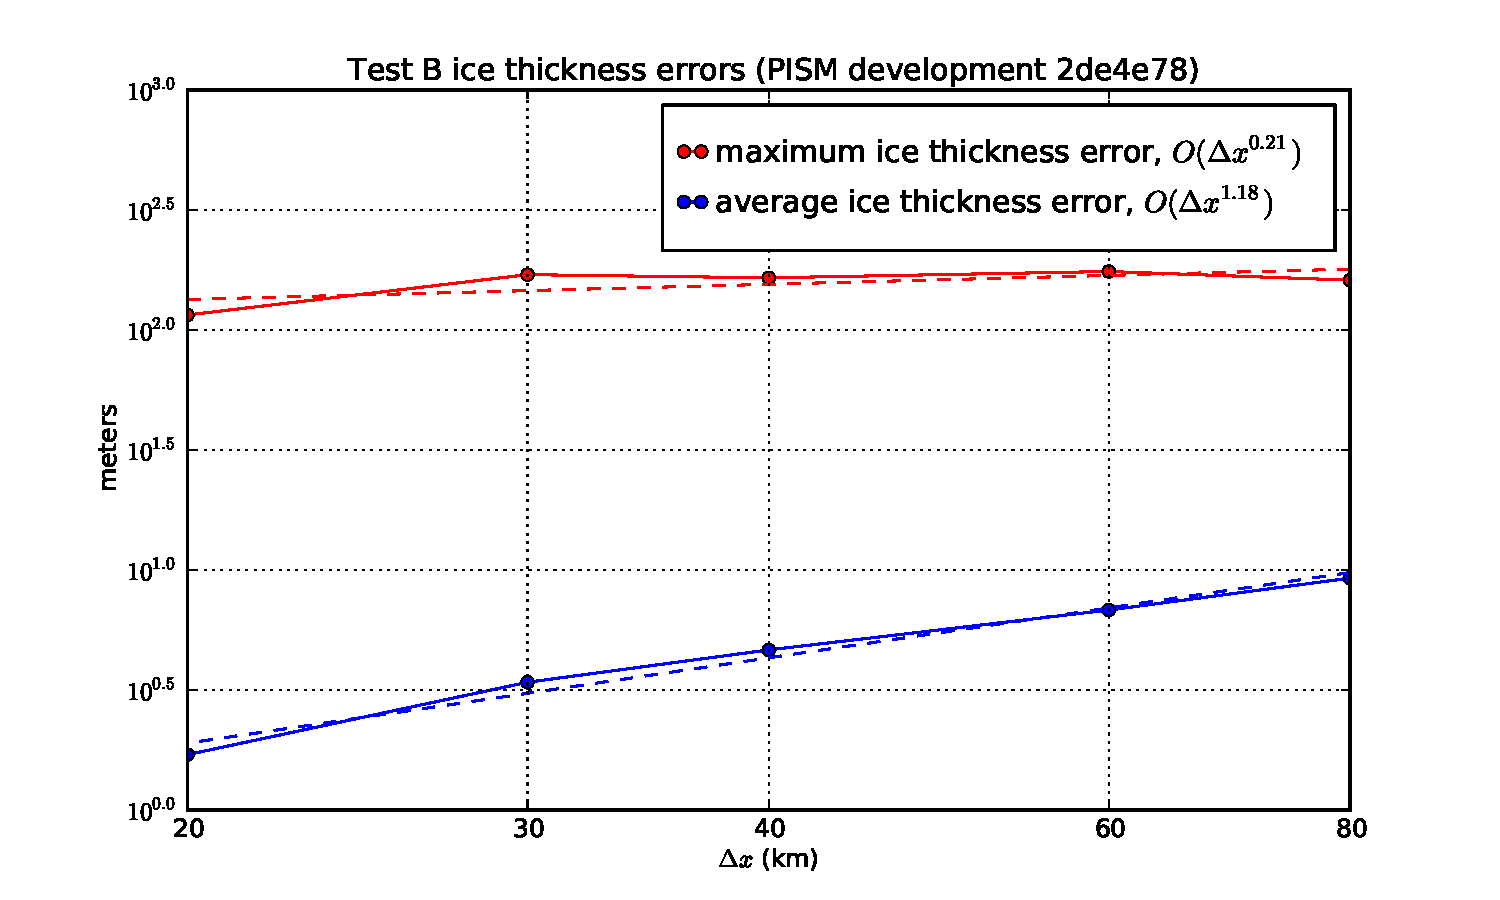
\includegraphics[width=5.0in,keepaspectratio=true]{test-B-thickness}
\caption{Numerical thickness errors in test B. See \cite{BLKCB} for discussion.}
\label{fig:thickerrsB}
\end{figure}

\begin{figure}[ht]
\centering
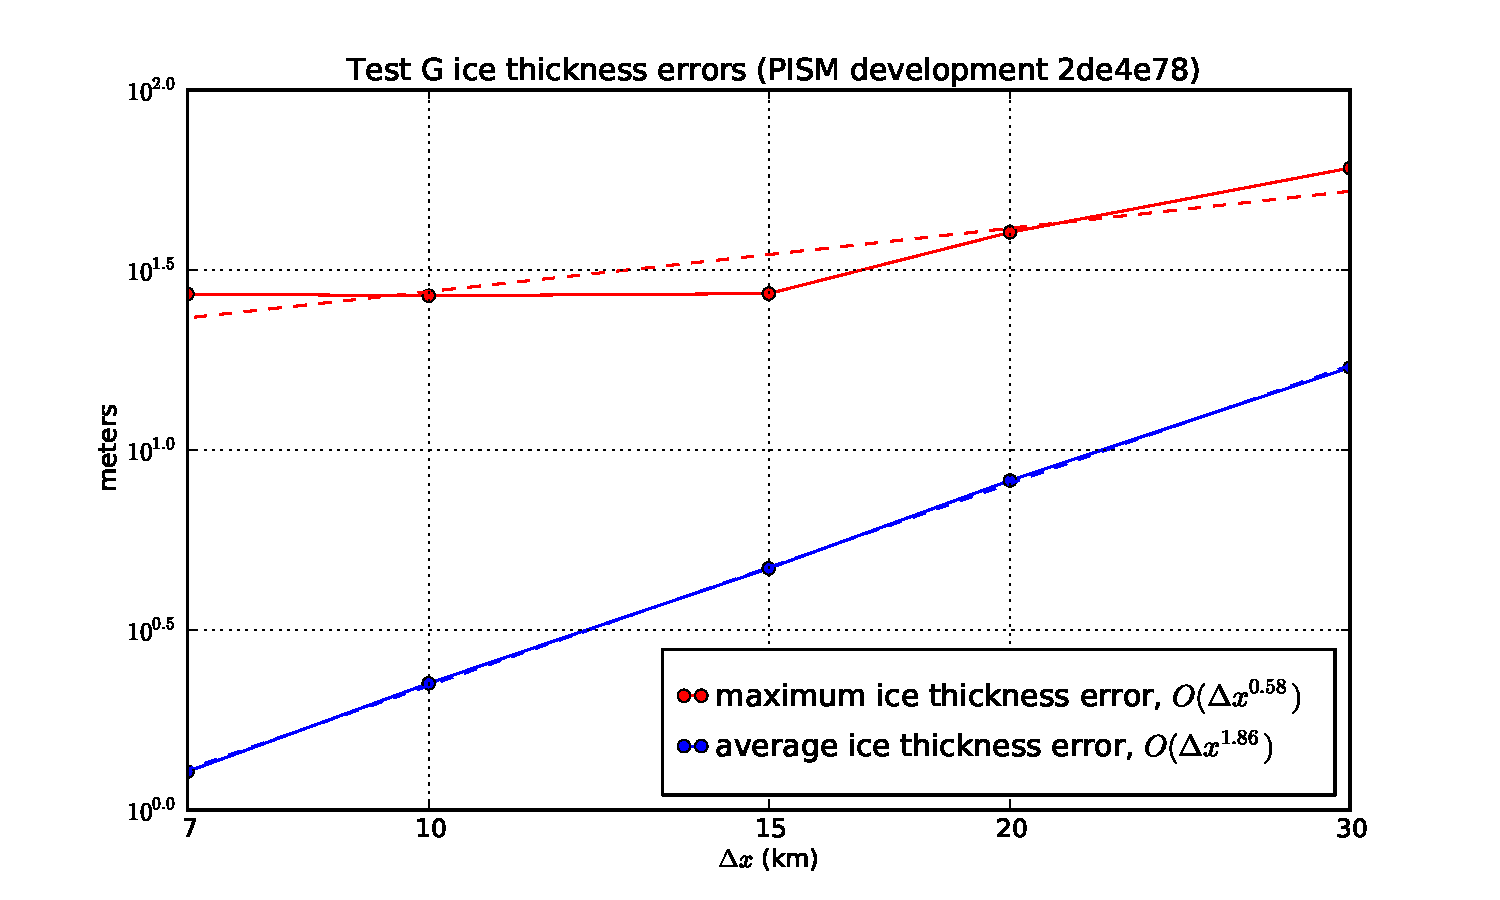
\includegraphics[width=5.0in,keepaspectratio=true]{test-G-thickness}
\caption{Numerical thickness errors in test G.  See \cite{BBL} and \cite{BLKCB}.}
\label{fig:thickerrsG}
\end{figure}

\begin{figure}[ht]
\centering
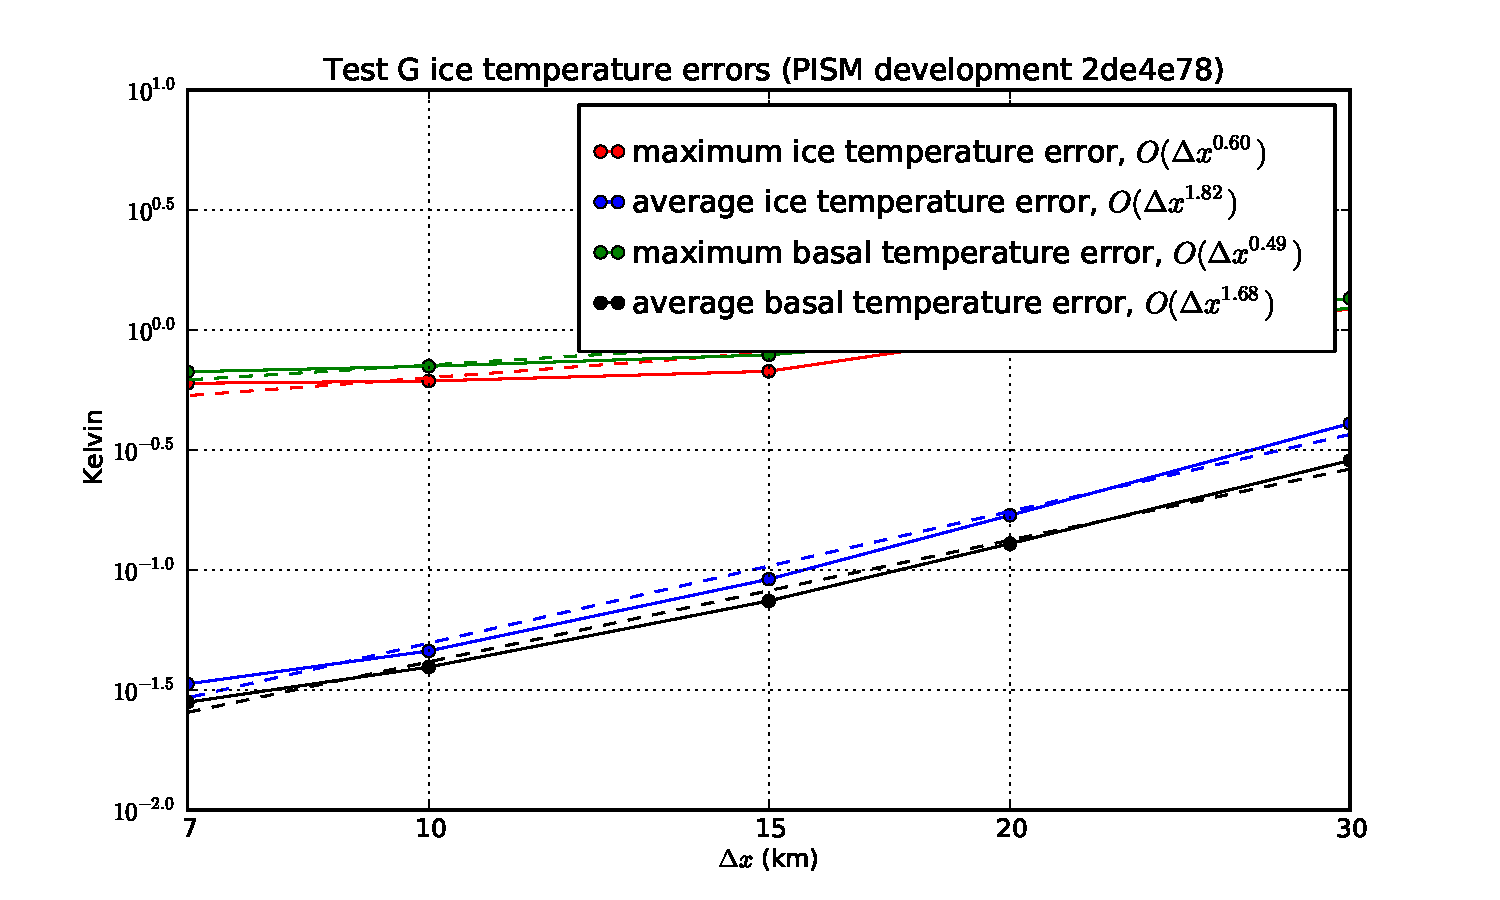
\includegraphics[width=5.0in,keepaspectratio=true]{test-G-temp}
\caption{Numerical temperature errors in test G. See \cite{BBL}.}
\label{fig:temperrsG}
\end{figure}

\begin{figure}[ht]
\centering
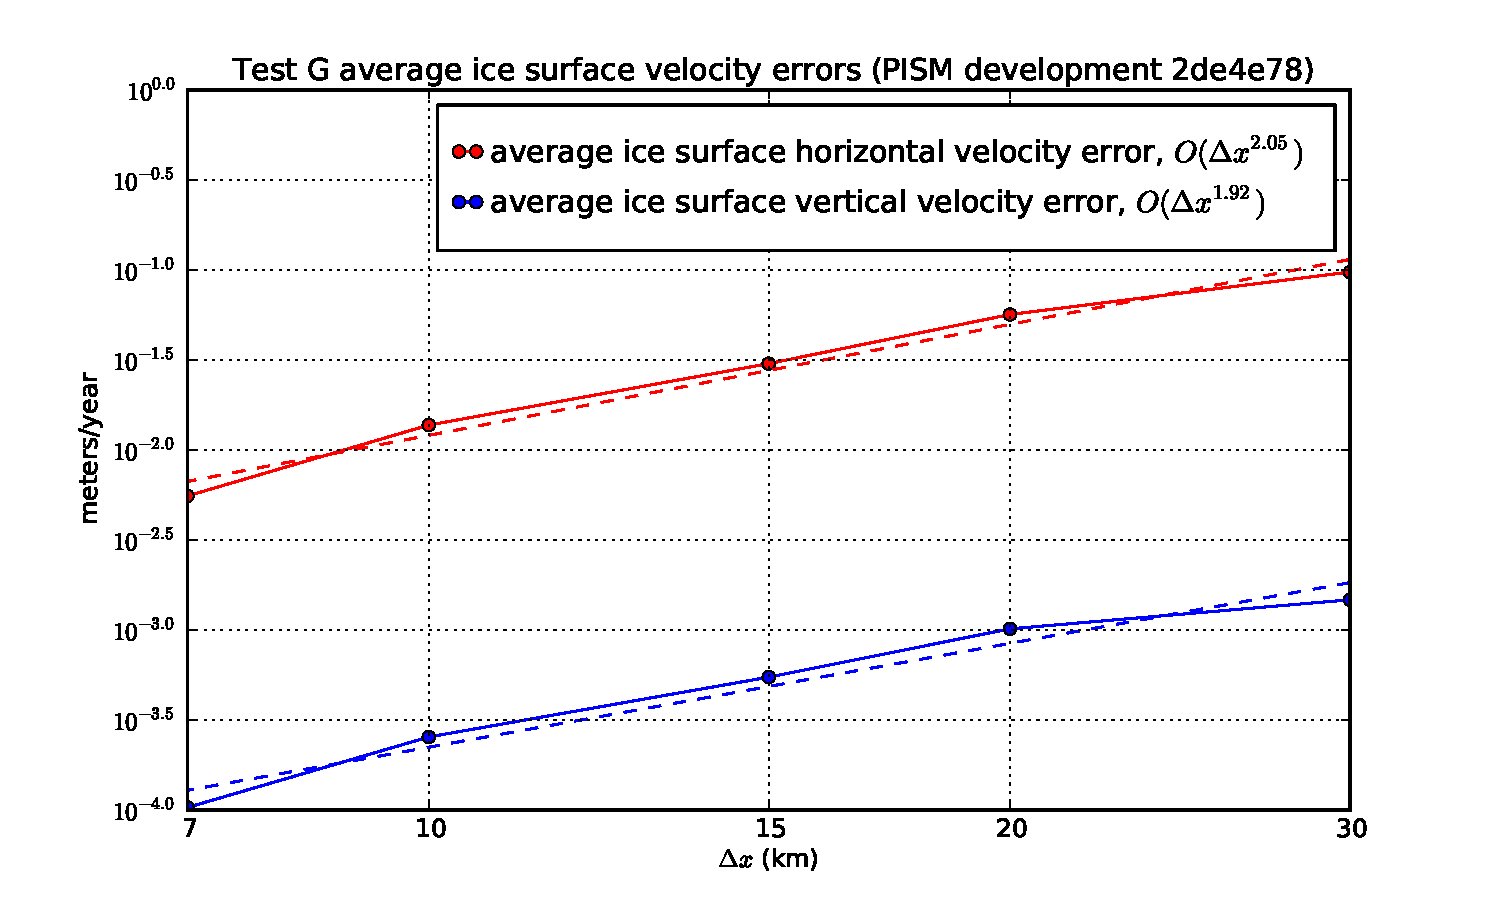
\includegraphics[width=5.0in,keepaspectratio=true]{test-G-surfvels}
\caption{Numerical errors in computed surface velocities in test G.}
\label{fig:surfvelerrsG}
\end{figure}

\begin{figure}[ht]
\centering
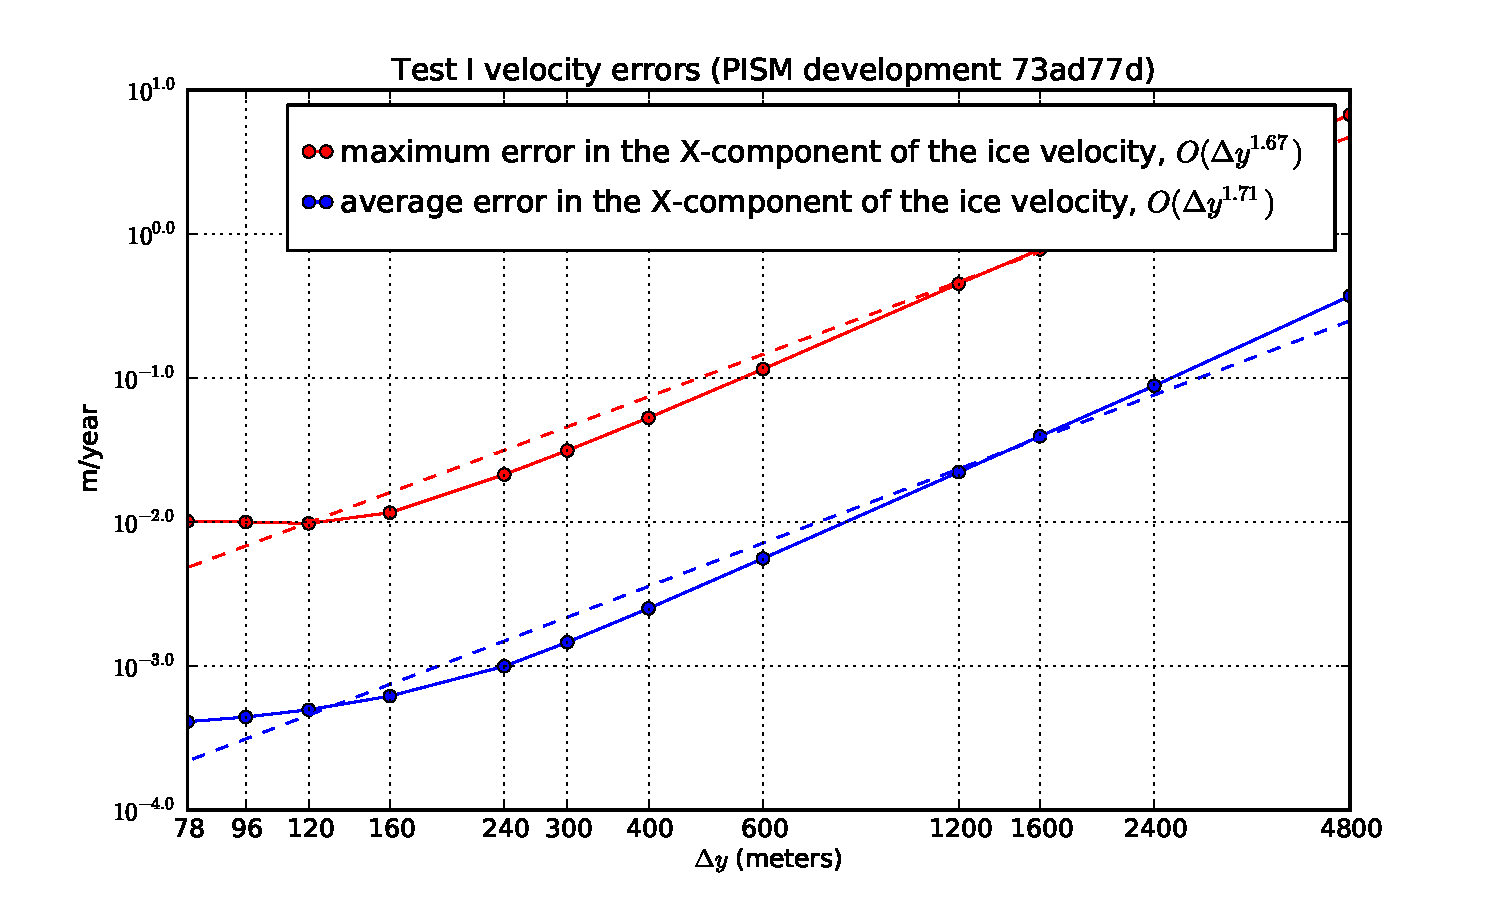
\includegraphics[width=5.0in,keepaspectratio=true]{test-I-errors}
\caption{Numerical errors in horizontal velocities in test I, an ice stream. See \cite{SchoofStream,BBssasliding}.}
\label{fig:velerrsI}
\end{figure}

%%% Local Variables: 
%%% mode: latex
%%% TeX-master: "manual"
%%% End: 


\clearpage\newpage

\section{Simplified geometry experiments with PISM}\label{sec:simp}

There have been three stages of ice sheet model intercomparisons based on simplified geometry experiments since the early 1990s \cite{BuelerSpray}.\index{EISMINT!defined}

EISMINT I \cite[ European Ice Sheet Modeling INiTiative]{EISMINT96}\footnote{See \url{http://homepages.vub.ac.be/\%7Ephuybrec/eismint.html}.} was the first of these and involved only the isothermal shallow ice approximation (SIA).  Both fixed margin and moving margin experiments were performed in EISMINT I, and various conclusions were drawn about the several numerical schemes used in the intercomparison.  EISMINT I is superceded, however, by verification using the full variety of known exact solutions to the isothermal SIA \cite{BLKCB}.  The ``rediscovery'', since EISMINT I, of the Halfar similarity solution with zero accumulation \cite{Halfar83}, and verification runs using that solution, already suffices to measure the isothermal SIA performance of PISM more precisely than would be allowed by comparison to EISMINT I results.

EISMINT II \cite{EISMINT00} pointed out interesting and surprising properties of the thermocoupled SIA.  References \cite{BBL,Hindmarsh04,Hindmarsh06,PayneBaldwin,SaitoEISMINT,BBssasliding} each interpret the EISMINT II experiments and/or describe attempts to add more complete physical models to ``fix'' the (perceived and real) shortfalls of ice sheet model behavior on EISMINT II experiments.  We believe that the discussion in \cite{PayneDongelmans,PayneBaldwin,BBL} adequately explains the ``spokes'' in EISMINT II experiment F as a genuine fluid instability, while \cite{Fowler01} and Appendix B of \cite{BBssasliding} adequately cautions against the continuum model that generates the ``spokes'' in EISMINT II experiment H.   Thus we can move on from that era of controversy.  In any case, PISM has built-in support for all of the published and unpublished EISMINT II experiments; these are described in the next subsection.

The ISMIP (Ice Sheet Model Intercomparison Project)\footnote{See \url{http://homepages.vub.ac.be/\%7Ephuybrec/ismip.html}.}\index{ISMIP!defined} round of intercomparisons covers 2008--2013 (at least).  There are four components of ISMIP substantially completed, namely HOM = Higher Order Models \cite{ISMIPHOM,HOMelmer}, HEINO = Heinrich Event INtercOmparison \cite{GreveTakahamaCalov,Calovetal2009HEINOfinal}, MISMIP (below), and MISMIP3d (also below).

PISM participated in HEINO, but this ability is unmaintained.   We believe\index{ISMIP!interpretation of HEINO results} the continuum problem described by HEINO, also used in EISMINT II experiment H (above), is not meaningfully approximate-able because of a required discontinuous jump in the basal velocity field.  The continuum problem predicts infinite vertical velocity because of this jump \cite[Appendix B]{BBssasliding}.  Details of the numerical schemes and their results are irrelevant if the continuum model makes such a prediction.  PISM offers the physical continuum model described in \cite{BBssasliding}, an SIA+SSA hybrid, as an alternative to the continuum model used in ISMIP-HEINO and EISMINT II experiment H.  Indeed the SIA+SSA hybrid is offered as a unified shallow model for real ice sheets (section \ref{sec:dynamics}).

There is no current plan to support ISMIP-HOM \cite{ISMIPHOM,HOMelmer}, but comparison of shallow PISM results to exact Stokes solutions is a goal for PISM evaluation.

A third and fourth ISMIP parts are the two parts of the Marine Ice Sheet Model Intercomparison Project, MISMIP\index{ISMIP!MISMIP} \cite{MISMIP2012} and MISMIP3D\index{ISMIP!MISMIP3d} \cite{MISMIP3d2013}.  These experiments are supported in PISM, as described in subsections \ref{subsect:MISMIP} and \ref{subsect:MISMIP3d} below.


\subsection{EISMINT II}\label{subsect:EISMINTII}
\optsection{EISMINT II}

There are seven experiments described in the published EISMINT II writeup \cite{EISMINT00}.\index{EISMINT}  They are named A, B, C, D, F, G, and H.  They have these common features:\begin{itemize}
\item runs are for 200,000 years, with no prescribed time step;
\item a $61\times 61$ horizontal grid on a square domain ($1500$ km side length) is prescribed;
\item surface inputs (temperature and mass balance) have angular symmetry around the grid center;
\item the bed is flat and does not move (no isostasy);
\item the temperature in the bedrock is not modeled;
\item only the cold (not polythermal) thermomechanically-coupled SIA is used \cite{EISMINT00}; and
\item basal melt rates do not affect the evolution of the ice sheet.
\end{itemize}
The experiments differ from each other in their various combinations of surface temperature and mass balance parameterizations.  Experiments H and G involve basal sliding, under the physically-dubious SIA sliding rubric \cite[Appendix B]{BBssasliding}, while the others don't.  Four experiments start with zero ice (A,F,G,H), while the other experiments (B,C,D) start from the final state of experiment A.

In addition to the seven experiments published in \cite{EISMINT00}, there were an additional five experiments described in the EISMINT II intercomparison description 
\cite{EISIIdescribe}, labeled E, I, J, K, and L.\index{EISMINT!unpublished additional EISMINT II experiments}  These experiments share most features listed above, but with the following differences.  Experiment E is the same as experiment A except that the peak of the accumulation, and also the low point of the surface temperature, are shifted by 100 km in both $x$ and $y$ directions; also experiment E starts with the final state of experiment A.  Experiments I and J are similar to experiment A but with non-flat ``trough'' bed topography.  Experiments K and L are similar to experiment C but with non-flat ``mound'' bed topography.

See table \ref{tab:eisII} for how to run all EISMINT II experiments in PISM.  Note that the vertical grid is not specified in EISMINT II, but it seems that good simulation of the thermomechanically-coupled conditions near the base of the ice requires relatively-fine resolution there.  (It is difficult to be quantitative because of a lack of theory.)  We suggest using the default unequally-spaced grid with 61 levels, which gives a grid spacing of 18 m in the ice layer closest to the bed.  Alternatively these experiments can be done with an equally-spaced grid; in this case we suggest using 201 vertical levels to give 20 m spacing, for example.

These SIA-only simulations parallelize well.  Very roughly, for the standard $61\times 61$ horizontal grid, wall-clock-time speedups will occur up to about 30 processors.  Runs on finer (horizontal) grids will benefit from even more processors.

Table \ref{tab:eisII} shows how all EISMINT II experiments are done in PISM.  Experiments below the horizontal line in Table \ref{tab:eisII} are only documented in \cite{EISIIdescribe}.

\begin{table}[ht]
\centering
\small
\begin{tabular}{@{}llll}\toprule
\textbf{Command: ``\texttt{pisms }'' $+$} & \textbf{Relation to experiment A} \\
\midrule
\texttt{-eisII A -Mx 61 -My 61 -Mz 61 -y 200000 -o eisIIA.nc} & \\
\texttt{-eisII B -i eisIIA.nc -y 2e5 -o eisIIB.nc} & warmer \\
\texttt{-eisII C -i eisIIA.nc -y 2e5 -o eisIIC.nc} & less snow (lower accumulation)\\
\texttt{-eisII D -i eisIIA.nc -y 2e5 -o eisIID.nc} & smaller area of accumulation \\
\texttt{-eisII F -Mx 61 -My 61 -Mz 61 -y 2e5 -o eisIIF.nc} & colder; famous spokes \cite{BBL} \\
\texttt{-eisII G -Mx 61 -My 61 -Mz 201 -y 2e5 -o eisIIG.nc} & sliding (regardless of temperature) \\
\texttt{-eisII H -Mx 61 -My 61 -Mz 201 -y 2e5 -o eisIIH.nc} & melt-temperature activated sliding \\ \midrule
\texttt{-eisII E -i eisIIA.nc -y 2e5 -o eisIIE.nc} & shifted climate maps \\
\texttt{-eisII I -Mx 61 -My 61 -Mz 201 -y 2e5 -o eisIII.nc} & trough topography \\
\texttt{-eisII J -i eisIII.nc -y 2e5 -o eisIIJ.nc} & trough topography and less snow \\
\texttt{-eisII K -Mx 61 -My 61 -Mz 201 -y 2e5 -o eisIIK.nc} & mound topography \\
\texttt{-eisII L -i eisIIK.nc -y 2e5 -o eisIIL.nc} & mound topography and less snow \\
\bottomrule
\normalsize
\end{tabular}
\caption{Running the EISMINT II experiments in PISM.\index{PISM!running the EISMINT II experiments in}  Use \texttt{-skip -skip_max 5}, on the $61\times 61$ default grid, for significant speedup.}
\label{tab:eisII}
\end{table}

The EISMINT II experiments can be run with various modifications of the default settings.  Of course the grid can be refined.  For instance, a twice as fine grid in the horizontal is ``\texttt{-Mx 121 -My 121}''.  Table \ref{tab:eisIIoptions} lists some optional settings which are particular to the EISMINT II experiments.

\begin{table}[ht]
\centering
\small
\begin{tabular}{@{}lllp{0.45\linewidth}}\toprule
\textbf{Option} & \textbf{Default values [expers]} & \textbf{Units} & \textbf{Meaning} \\\midrule
\intextoption{eisII} & A & &  Choose single character name of EISMINT II \cite{EISMINT00} simplified geometry experiment.  See Table \ref{tab:eisII}. \\
\intextoption{Mmax} & 0.5 [ABDEFGHIK], 0.25 [CJL] & m$/$a & max value of accumulation rate \\
\intextoption{Rel} & 450 [ABEFGHIK], 425 [CDJL] & km & radial distance to equilibrium line \\
\intextoption{Sb} & $10^{-2}$ [\emph{all}] & (m/a)/km & radial gradient of accumulation rate \\
\intextoption{ST} & $1.67 \times 10^{-2}$ [\emph{all}] & K/km & radial gradient of surface temperature\\
\intextoption{Tmin} & 238.15 [ACDEGHIJKL], & K & max of surface temperature \\
 & 243.15[B], 223.15[F] & & \\
\intextoption{bmr_in_cont} & & & Include the basal melt rate in the mass continuity computation; overrides EISMINT II default. \\
\bottomrule\normalsize
\end{tabular}
\caption{Changing the default settings for EISMINT II}
\label{tab:eisIIoptions}
\end{table}

In PISM the height of the computational box, the quantity set by \texttt{-Lz}, is set at the beginning of the run.  It is chosen for the EISMINT II experiments according to the observed maximum values occuring in standard runs.  If the ice thickens beyond the chosen level for the top of the computational box then additional layers are automatically added to the computational grid.  In fact, if the ice grows above the height of the computational box then a message appears, \texttt{PISM WARNING: max ice thickness ... is greater than the height of the computational box ...}, and then at least two additional levels are added to the vertical grid.  However, in general this mechanism can run away to use up all memory in extreme cases so, if the height of the computational box grows so large that the grid has more than twice the original number of vertical levels, then PISM produces an error message and stops.   Therefore it is possible that the number of vertical levels at the end of the run exceeds the initial \texttt{-Mz} value.  Setting EISMINT II options \texttt{-Mmax} or \texttt{-Sb} to produce higher accumulation rates than the default values (see table \ref{tab:eisIIoptions}) may cause the ice sheet to thicken above the standard thickness and therefore trigger this automatic extension mechanism.  Similarly, colder ice caused by nonstandard \texttt{-Tmin} or \texttt{-ST} values can produce unusually thick ice.  The user may always choose to use a larger, more conservative value for option \texttt{-Lz}, however.

See subdirectory \verb|examples/eismintII/| for a simple helper script \verb|runexp.sh|.


\subsection{MISMIP}\label{subsect:MISMIP}
\optsection{MISMIP}\index{ISMIP!MISMIP}

This intercomparison addresses grounding line dynamics by considering an idealized one-dimensional stream-shelf system.  In summary, a flowline ice stream and ice shelf system is modeled, the reversibility of grounding line movement under changes in the ice softness is tested, different sliding laws are tested, and the behavior of grounding lines on reverse-slope beds is tested.  The intercomparison process is described at the website

\centerline{\url{http://homepages.ulb.ac.be/~fpattyn/mismip/}}

\noindent Find a full text description there, along with the published report on the results \cite{MISMIP2012}; that paper includes results from PISM version 0.1.  These documents are essential reading for understanding MISMIP results generally, and for appreciating the brief discussion in this subsection.

PISM's version of MISMIP includes an attached ice shelf even though modeling the shelf is theoretically unnecessary in the flow line case.  The analysis in \cite{SchoofMarine1} shows that the only effect of an ice shelf, in the flow line case, is to transfer the force imbalance at the calving front directly to the ice column at the grounding line.  Such an analysis does not apply to ice shelves with two horizontal dimensions; real ice shelves have ``buttressing'' and ``side drag'' and other forces not present in the flow line \cite{Goldbergetal2009}.  See the next subsection on MISMIP3d and the Ross ice shelf example in section \ref{sec:ross}, among other examples.

We must adapt the usual 3d PISM model to two horizontal dimensions, i.e.~to do flow-line problems (see section \ref{sec:flowline-modeling}).  The flow direction for MISMIP is taken to be ``$x$''.  We periodize the cross-flow direction ``$y$'', and use the minimum number of points in the $y$-direction.  This number turns out to be ``\texttt{-My 3}''; fewer points than this in the cross-flow direction confuses the finite difference scheme.

PISM can do MISMIP experiments with either of two applicable ice dynamics models.  Model 1 is a pure SSA model; ``category 2'' in the MISMIP classification.  Model 2 combines SIA and SSA velocities as described in \cite{Winkelmannetal2011}; ``category 3'' because it resolves ``vertical'' shear (i.e.~using SIA flow).

There are many runs for a complete MISMIP intercomparison submission.  Specifically, for a given model there are $62$ runs for each grid choice, and three (suggested) grid choices, so a full suite is $3 \times 62 = 186$ runs.

The coarsest grid (``mode 1'') has 12 km spacing.  The finest grid, ``mode 2'' with 1.2 km spacing, accounts for all the compute time, however; in the MISMIP description it is 1500 grid spaces in the flow line direction (= 3001 grid \emph{points} in PISM's doubled computational domain).  In between is ``mode 3'', a mode interpretable by the intercomparison participant, and here we just use a 6 km grid.

The implementation of MISMIP in PISM conforms to the intercomparison description, but that document specifies
\begin{quotation}
\dots we require that the rate of change of grounding line position be $0.1$ m/a or less, while the rate of change of ice thickness at each grid point at which ice thickness is defined must be less than $10^{-4}$ m/a \dots
\end{quotation}
as a standard for ``steady state''.  The scripts here do not implement this stopping criterion.  However, we report enough information, in PISM output files with scalar and spatially-variable time-series, to compute a grounding line rate or the time at which the thickness rate of change drops below $10^{-4}$ m/a.

See

  \centerline{\texttt{examples/mismip/mismip2d/README.md}}

\noindent for usage of the scripts that run MISMIP experiments in PISM.  For example, as described in this \texttt{README.md}, the commands

\begin{verbatim}
$ ./run.py -e 1a --mode=1 > experiment-1a-mode-1.sh
$ bash experiment-1a-mode-1.sh 2 >& out.1a-mode-1 &
$ ./plot.py ABC1_1a_M1_A7.nc -p -o profileA7.png
\end{verbatim}

\noindent first generate a bash script, then use it to do a run which takes about 20 minutes, and then generate an image in \texttt{.png} format.  Note that step 7 is in the middle of the experiment.  It is shown in Figure \ref{fig:MISMIPmodel1exper1aA7} (left).
 
\begin{figure}[ht]
\centering
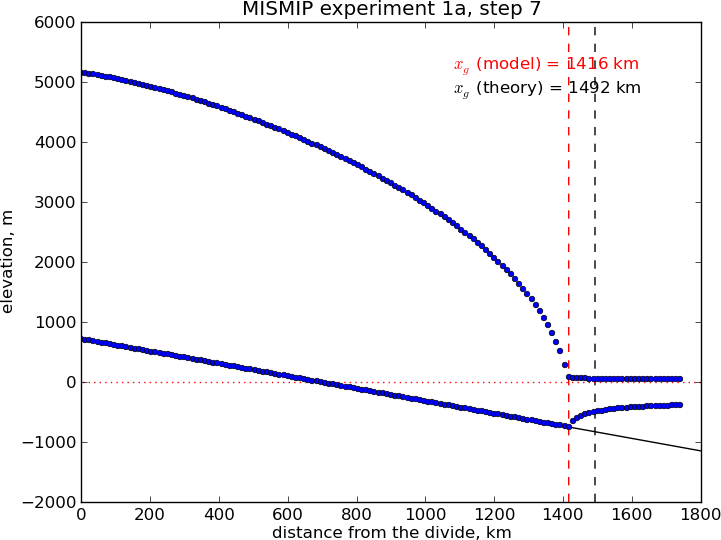
\includegraphics[width=3.3in,keepaspectratio=true]{profileA7} \,
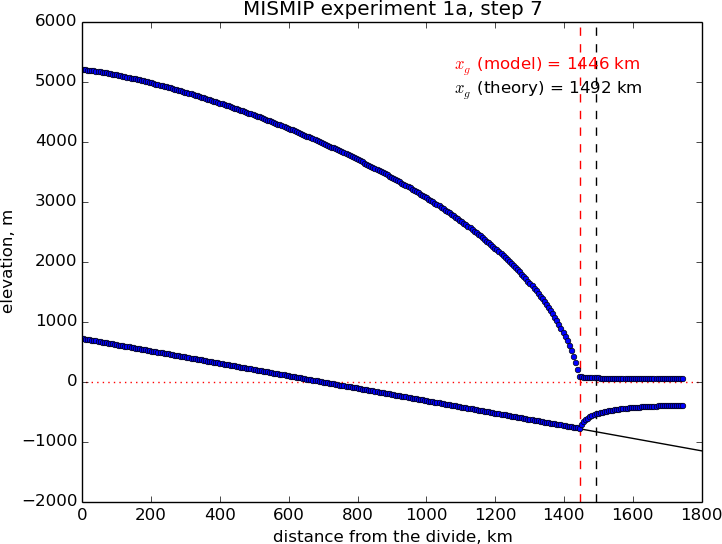
\includegraphics[width=3.3in,keepaspectratio=true]{profileA7-M3}
\caption{A marine ice sheet profile in the MISMIP intercomparison; PISM model 1, experiment 1a, at step 7.  Left: grid mode 1 (12 km grid).  Right: grid mode 3 (6 km grid).}
\label{fig:MISMIPmodel1exper1aA7}
\end{figure}

\begin{figure}[ht]
\centering
\includegraphics[width=4.0in,keepaspectratio=true]{SM-1a-A1}
\caption{Analytical profile for steady state of experiment 1a, step 1, from theory in \cite{SchoofMarine1}.  This is a boundary layer asymptotic matching result, but not the exact solution to the equations.}
\label{fig:SMexper1aM1A1}
\end{figure}

The script \texttt{MISMIP.py} in \texttt{examples/mismip/mismip2d} has the ability to compute the profile from the Schoof's \cite{SchoofMarine1} asymptotic-matching boundary layer theory.  This script is a Python translation, using \texttt{scipy} and \texttt{pylab}, of the \Matlab codes in \url{http://homepages.ulb.ac.be/~fpattyn/mismip/MISMIP_distribution.tar}.  For example,

\begin{verbatim}
$ python MISMIP.py -o mismip_analytic.png
\end{verbatim}
 
\noindent produces a \verb|.png| image file with Figure \ref{fig:SMexper1aM1A1}.  By default \texttt{run.py} uses the asymptotic-matching thickness result from the \cite{SchoofMarine1} theory to initialize the initial ice thickness, as allowed by the MISMIP specification.

\begin{figure}[ht]
\centering
\includegraphics[width=3.3in,keepaspectratio=true]{profileA7-M2}
\caption{Results from MISMIP grid mode 2, with 1.2 km spacing, for steady state of experiment 1a: profile at step 7 (compare Figure \ref{fig:MISMIPmodel1exper1aA7}).}
\label{fig:MISMIPmode2results}
\end{figure}

Generally the PISM result does not put the grounding line in the same location as Schoof's boundary layer theory, and at least at coarser resolutions the problem is with PISM's numerical solution, not with Schoof's semi-analytic theory.  The result improves under grid refinement, however.  Results from grid mode 3 with 6 km spacing, instead of 12 km in mode 1, are the right part of Figure \ref{fig:MISMIPmodel1exper1aA7}.  The corresponding results from grid mode 2, with 1.2 km spacing, are in Figure \ref{fig:MISMIPmode2results}.  Note that the difference between the numerical grounding line location and the semi-analytical location has been reduced from 76 km for grid mode 1 to 16 km for grid mode 2 (a factor of about 5), by using a grid refinement from 12 km to 1.2 km (a factor of about 10).


\subsection{MISMIP3d}\label{subsect:MISMIP3d}
\optsection{MISMIP3d}\index{ISMIP!MISMIP3d}
The ice2sea MISMIP3d intercomparison is a two-horizontal-dimensional extension of the flowline case described above.  As before, in MISMIP3d the grounding line position and its reversibility under changes of physical parameters is analyzed.  Instead of changing the ice softness, however, the spatial distribution and magnitude of basal friction is adjusted between experiments.  The applied basal friction perturbation of the basal friction is a localized gaussian ``bump'' and thus a curved grounding line is obtained.  In contrast to the flowline experiments, no (semi-)analytical solutions are available to compare to the numerical results.

A full description of the MISMIP3d experiments can be found at

\centerline{\url{http://homepages.ulb.ac.be/~fpattyn/mismip3d/}}

\noindent and the results are published in \cite{MISMIP3d2013}.

A complete set of MISMIP3d experiments consists of three runs: Firstly, a flowline solution on a linearly-sloped bed, similar to the flowline MISMIP experiments of the previous section, is run into a steady state (``standard experiment \texttt{Stnd}'').  Then the localized sliding perturbation is applied (``perturbation experiment'')  causing the grounding line to shift and lose symmetry.  Two different amplitudes of the perturbation are considered (``\texttt{P10}'' and ``\texttt{P75}'').  Finally, beginning from the final state of the perturbation experiment, the sliding perturbation is removed and the system is run again into steady state (``reversibility experiment'').  The resulting geometry, in particular the grounding line position, is expected to be close to that of the standard experiment.  Expecting such reversibility assumes that a particular stationary ice geometry only depends on its physical parameters and boundary conditions and not on how it is dynamically reached.

For these experiments in PISM, a Python script generates a shell script which has the commands and options for running a MISMIP3d experiment.  The python script is \texttt{createscript.py} in the folder \texttt{examples/mismip/mismip3d/}.  Run

\begin{verbatim}
$ ./createscript.py -h
\end{verbatim}

\noindent to see a usage message.  A \texttt{README.md} gives a tutorial on how to use \texttt{createscript.py} and do the runs themselves.

For the flowline \texttt{Stnd} experiment, as in the MISMIP case, a computational domain with three grid points in the direction orthogonal to the ice flow (arbitrarily chosen as y-direction) is chosen by \texttt{createscript.py}.  For the perturbation and reversibility experiments a domain is defined which is symmetric along the ice-divide (mirror symmetry) and along the center line of the ice flow, while the side boundaries are periodic, which corresponds to a free-slip condition for the flow in x-direction. Though this choice of the symmetric computational domain increases computational cost, it allows us to use standard PISM without fixing certain boundary conditions in the code.  (That is, it avoids the issues addressed in the regional mode of PISM; see section \ref{sec:jako}.)

PISM participated in the MISMIP3d intercomparison project \cite{MISMIP3d2013} using version \texttt{stable0.5}, and the exact results can be reproduced using that version.  PISM's results, and the role of resolution and the new subgrid grounding line interpolation scheme are discussed in \cite{Feldmannetal2014}.

We observed a considerable improvement of the results with respect to the absolute grounding line positions compared to other models (e.g. the FE reference model Elmer/Ice) and to the reversibility when applying the subgrid grounding line interpolation method; see Figure \ref{fig:Subgl}.  Furthermore, we observed that only using SSA yields almost the same results as the full hybrid SIA+SSA computation for the MISMIP3D (and also the MISMIP) experiments, but, when not applying the SIA computation, after a considerably shorter computation time (about 10 times shorter).  We explain the small and almost negligible SIA velocities for the MISMIP(3D) experiments with the comparably small ice surface gradients in the MISMIP3d ice geometries.  See Fig.~\ref{fig:compSIASSA} for a comparison of SSA and SIA velocities in the MISMIP3D geometry.  Note that both Figures \ref{fig:Subgl} and \ref{fig:compSIASSA} were generated with resolution of $\Delta x = \Delta y = 1\;$km.

\begin{figure}[ht]
\centering
\includegraphics[width=3.3in,keepaspectratio=true]{Subgl}
\includegraphics[width=3.3in,keepaspectratio=true]{NoSubgl}
\caption{Comparison between the grounding lines of the higher-amplitude (``\texttt{P75}'') MISMIP3d experiments performed with PISM when using the subgrid grounding line interpolation method (left) or not using it (right).  In both cases the SIA+SSA hybrid is used.}
\label{fig:Subgl}
\end{figure}

\begin{figure}[ht]
\centering
\includegraphics[width=5.0in,keepaspectratio=true]{comp-SIA-SSA}
\caption{The SIA velocities are negligible in the MISMIP3d standard experiment (``\texttt{Stnd}'').  The steady state ice geometry is plotted (black) together with the computed SSA velocity (red) and SIA velocity (blue). The SIA velocity reaches its maximum value of about $10\,$m/a at the grounding line, about two orders of magnitude less than the maximum of the SSA velocity.}
\label{fig:compSIASSA}
\end{figure}

%%% Local Variables: 
%%% mode: latex
%%% TeX-master: "manual"
%%% End: 


\clearpage\newpage

\section{Validation case studies}\label{sec:validation} 

``Validation'' describes the comparison of numerical model output with physical observations in cases where the observations are sufficiently-complete and of sufficient quality so that the performance of the numerical model can be assessed \cite{Roache,Wesseling}.  Roughly speaking, validation can happen when the observations or data are better than the model, so the comparison measures the quality of the numerical model and not merely errors in, or incompleteness of, the data.  Because of the difficulty of measuring boundary conditions for real ice flows, this situation is not automatic in glaciology, or even common.\footnote{Which explains the rise of ``simplified geometry intercomparisons''; see section \ref{sec:simp}.}  Nonetheless we try two cases, first where PISM is applied on millimeter scale to model a laboratory experiment, and second for a large-scale ice flow in which all uncertainties of bedrock topography, basal sliding, and subglacial hydrology are removed, namely a present-day ice shelf.

\subsection{An SIA flow model for a table-top laboratory experiment}\label{sec:labgum}
\index{PISM!validation of SIA flow model} \index{validation!SIA flow model}

Though there are additional complexities to the flow of real ice sheets, an ice sheet is a shear-thinning fluid with a free surface.  PISM ought to be able to model such flows in some generality.  We test that ability here by comparing PISM's isothermal SIA numerical model to a laboratory observations of a 1\% Xanthan gum suspension in water in a table-top, moving-margin experiment by R.~Sayag and M.~Worster \cite{SayagWorster2013,SayagPeglerWorster2012}.  The ``gum'' fluid is more shear-thinning than ice, and it has much lower absolute viscosity values, but it has the same density.  This flow has total mass $\sim 1$ kg, compared to $\sim 10^{18}$ kg for the Greenland ice sheet.

We compare our numerical results to the ``constant-flux'' experiment from \cite{SayagWorster2013}.  Figure \ref{fig:labgumexperiment} shows the experimental setup by reproducing Figures 2(c) and 2(d) from that reference.  A pump pushes the translucent blue-dyed fluid through a round 8 mm hole in the middle of a clear table-top at a mass rate of about 3 gm/s.  The downward-pointing camera, which produced the right-hand figure, allows measurement of the location of margin of the ``ice cap'', and in particular of its radius.  The measured radii data are the black dots in Figure \ref{fig:labgumresult}.

\begin{figure}[ht]
\centering
\includegraphics[width=6.0in,keepaspectratio=true]{labgumexperiment}
\caption{Reproduction of Figures 2(c) and 2(d) from \cite{SayagWorster2013}.  Left: experimental  apparatus used for ``constant-flux release'' experiment.  Right: snapshot of constant-flux experiment (plan view), showing an axisymmetric front.}
\label{fig:labgumexperiment}
\end{figure}

The closest glaciological analog would be an ice sheet on a flat bed fed by positive basal mass balance (i.e.~``refreeze'') underneath the dome, but with zero mass balance elsewhere on the lower and upper surfaces.  However, noting that the mass-continuity equation is vertically-integrated, we may model the input flux (mass balance) as arriving at the \emph{top} of the ice sheet, to use PISM's climate-input mechanisms.  The flow though the input hole is simply modeled as constant across the hole, so the input ``climate'' uses \texttt{-surface given} with a field \texttt{climatic_mass_balance}, in the bootstrapping file, which is a positive constant in the hole and zero outside.  While our replacement of flow into the base by mass balance at the top represents a very large change in the vertical component of the velocity field, we still see good agreement in the overall shape of the ``ice sheet'', and specifically in the rate of margin advance.

Sayag \& Worster estimate Glen exponent $n = 5.9$ and a softness coefficient $A = 9.7 \times 10^{-9}\,\text{Pa}^{-5.9}\,\text{s}^{-1}$ for the flow law of their gum suspension, using regression of laboratory measurements of the radius.  (Compare PISM defaults $n=3$ and $A\approx 4\times 10^{-25}\,\text{Pa}^{-3}\,\text{s}^{-1}$ for ice.)  Setting the Sayag \& Worster values is one of several changes to the configuration parameters, compared to PISM ice sheet defaults, which are done in part by overriding parameters at run time by using the \texttt{-config_override} option.  See \texttt{examples/labgum/preprocess.py} for the generation of a configuration \texttt{.nc} file with these settings.

To run the example on the default 10 mm grid, first do
\begin{verbatim}
$ python preprocess.py
\end{verbatim}
%$ - match dollar signs to make emacs happy
and then do a run for 746 model seconds \cite{SayagWorster2013} on the 10 mm grid on a $520\,\text{mm}\,\times 520\,\text{mm}$ square domain using 4 processors:
\begin{verbatim}
$ ./rungum.sh 4 52 &> out.lab52 &
\end{verbatim}
%$ - match dollar signs to make emacs happy
This run generates text file \texttt{out.lab52}, diagnostic files \texttt{ts_lab52.nc} and \texttt{ex_lab52.nc}, and final output \texttt{lab52.nc}.  This run took about 5 minutes on a 2013 laptop, thus roughly real time!  When it is done, you can compare the modeled radius to the experimental data:
\begin{verbatim}
$ ./showradius.py -o r52.png -d constantflux3.txt ts_lab52.nc
\end{verbatim}
%$ - match dollar signs to make emacs happy

You can also redo the whole thing on higher resolution grids (here: 5 and 2.5 mm), here using 6 MPI processes if the runs are done simultaneously, and when it is done after several hours, make a combined figure just like Figure \ref{fig:labgumresult}:
\begin{verbatim}
$ ./preprocess.py -Mx 104 -o initlab104.nc
$ ./preprocess.py -Mx 208 -o initlab208.nc
$ ./rungum.sh 2 104 &> out.lab104 &
$ ./rungum.sh 4 208 &> out.lab208 &
$ ./showradius.py -o foo.png -d constantflux3.txt ts_lab*.nc
\end{verbatim}
%$ - match dollar signs to make emacs happy

\begin{figure}[ht]
\centering
\includegraphics[width=6.5in,keepaspectratio=true]{labgumradius}
\caption{Radius $r_N(t)$ for runs with 10 mm (\texttt{ts_lab52.nc}), 5 mm (\texttt{ts_lab104.nc}), and 2.5 mm (\texttt{ts_lab208.nc}) grids, compared to observations from Sayag \& Worster's \cite{SayagWorster2013} table-top ``ice cap'' (gravity current) made from a 1 \% Xanthan gum suspension, as shown in Figure \ref{fig:labgumexperiment}.}
\label{fig:labgumresult}
\end{figure}

We see that on the coarsest grid the modeled volume has ``steps'' because the margin advances discretely.  Note we are computing the radius by first computing the fluid-covered area $a$ on the cartesian grid, and then using $a=\pi r^2$ to compute the radius.

Results are better on finer grids, especially at small times, because the input hole has radius of only 8 mm.  Furthermore this ``ice cap'' has radius comparable to the hole for the first few model seconds.  The early evolution is thus distinctly non-shallow, but we see that increasing the model resolution reduces most of the observation-model difference.  In fact there is little need for ``higher-order'' stresses because the exact similarity solution of the shallow continuum equations, used by Sayag \& Worster, closely-fits the data even for small radius and time \cite[Figure 4]{SayagWorster2013}.

In any case, the large-time observations are very closely-fit by the numerical results at all grid resolutions.  We have used the Glen-law parameters $n,A$ as calculated by Sayag \& Worster, but one could do parameter-fitting to get the ``best'' values if desired.  In particular, roughly speaking, $n$ controls the slope of the results in Figure \ref{fig:labgumresult} and $A$ controls their vertical displacement.


\subsection{An SSA flow model for the Ross Ice Shelf in Antarctica}\label{sec:ross} \index{PISM!diagnostic Ross ice shelf model}\index{Ice Sheets!Antarctic ice sheet!Ross ice shelf} \index{PISM!validation of SSA ice shelf model}\index{validation!SSA ice shelf model} \index{Ross ice shelf}
\optsection{Ross ice shelf}

As part of the EISMINT series of intercomparisons, MacAyeal and others \cite{MacAyealetal} successfully validated early-1990s ice shelf numerical models using velocity data for the Ross ice shelf.  The data were from the RIGGS survey \cite{RIGGS2}, acquired in the period 1973--1978 and measured at a few hundred locations in a grid across the shelf.  Substantial modelling developments followed EISMINT-Ross, including inverse modeling to recover depth-averaged viscosity \cite{RommelaereMacAyeal} and parameter-sensitivity studies \cite{HumbertGreveHutter}.  Previous PISM versions set up the EISMINT-Ross flow model and performed the diagnostic computation, with RIGGS data for validation.

However, availability of rich new data sets for ice sheet modeling, including the ALBMAP v1 \cite{LeBrocqetal2010} ice sheet geometry, bedrock, and climate data set, and the radar-derived (InSAR) MEaSUREs Antarctica Velocity Map \cite{Rignotetal2011}, allows us to use more complete, recent, and higher-resolution data for the same basic job.  Furthermore one can extend the diagnostic Ross ice shelf calculation both to other ice shelves around Antarctica and to time-evolving (``prognostic'') cases using the eigencalving \cite{Levermannetal2012} mechanisms.

The scripts in this subsection are found in directory \texttt{examples/ross/}.  In summary, the script \texttt{preprocess.py} downloads data and builds a NetCDF input file for PISM.  For the diagnostic computation we document first, the script \texttt{run_diag.sh} (in subdirectory \texttt{examples/ross/diagnostic/}) runs PISM.  The script \texttt{plot.py} shows a comparison of observations and model results, as in Figure \ref{fig:rosspython}.

\subsubsection*{Preprocessing the data}  The script \texttt{preprocess.py} downloads ALBMAP and MEaSUREs NetCDF files using \texttt{wget}; these files total around 100 Mb.  Then it uses NCO to cut out the relevant portion of the grid and CDO to conservatively-interpolate the high-resolution (500 m) velocity data onto the coarser (5 km) geometry grid used in ALBMAP.  The script \texttt{nc2cdo.py} from directory \texttt{util/}, prepares the NetCDF file for the application of CDO, which requires complete projection information.  Do

\begin{verbatim}
$ cd examples/ross/
$ ./preprocess.py
\end{verbatim}
%$ - match dollar signs to make emacs happy

The NetCDF file \texttt{Ross_combined.nc} produced by \texttt{preprocess.py} contains ice thickness, bed elevations, surface temperature, net accumulation, as well as latitude and longitude values.  All of these are typical of ice sheet modelling data, both in diagnostic runs and as needed to initialize and provide boundary conditions for prognostic (evolutionary) runs; see below for the prognostic case with these data.  The \texttt{_combined} file also has variables \texttt{u_ssa_bc} and \texttt{v_ssa_bc} for the boundary values used in the (diagnostic and prognostic) computation of velocity.  They are used at all grounded locations and at ice shelf cells that are immediate neighbors of grounded ice.  The variable \texttt{bc_mask} specifies these locations.  Finally the variables \texttt{u_ssa_bc,v_ssa_bc}, which contain observed values, are used after the run to compare to the computed interior velocities.

\subsubsection*{Diagnostic computation of ice shelf velocity}  The diagnostic velocity computation bootstraps from \texttt{Ross_combined.nc} and does a zero-year run; in the $211\times 211$ grid case we demonstrate below, the key parts of the PISM command are

\begin{verbatim}
pismr -i ../Ross_combined.nc -bootstrap -Mx 211 -My 211 -Mz 3 -Lz 3000 -z_spacing equal \
    -surface given -stress_balance ssa -energy none -yield_stress constant -tauc 1e6 \
    -pik -ssa_dirichlet_bc -y 0 -ssa_e 0.6 -ssafd_ksp_monitor
\end{verbatim}
%$ - match dollar signs to make emacs happy

\noindent The computational grid here is the ``native'' $5$ km data grid used in ALBMAP.  Regarding the options,

\begin{itemize}
\item The maximum thickness of the ice is $2766$ m so we choose a height for the computational box large enough to contain the ice (i.e.~\texttt{-Lz 3000}).  Vertical grid resolution is, however, unimportant in this case because we use the SSA stress balance only, and the temperature set at bootstrapping suffices to determine the ice softness; thus the options \texttt{-Mz 3 -z_spacing equal -energy none}.

\item Option \texttt{-stress_balance ssa} selects the SSA stress balance and turns off the SIA stress balance computation, since our goal is to model the ice shelf.  It also side-steps a technical issue: PISM uses periodic boundary conditions at domain boundaries and most fields in this setup are not periodic.  Turning off SIA avoids operations such as differencing surface elevation across the domain edges.  For a more complete solution to this technical issue see section \ref{sec:jako} about a regional model using option \verb|-no_model_strip| and executable \verb|pismo|.

\item Option \texttt{-y 0} chooses a diagnostic run.

\item Option \texttt{-pik} is equivalent to \texttt{-cfbc -kill_icebergs} in this non-evolving example.  Note that \texttt{-kill_icebergs} removes effectively-detached bits of ice, especially in McMurdo sound area, so that the SSA problem is well-posed for the grounded-ice-sheet-connected ice shelf.

\item Option \intextoption{ssa_dirichlet_bc} forces the use of fields \texttt{u_ssa_bc,v_ssa_bc,bc_mask} described above.  The field \texttt{bc_mask} is $1$ at boundary condition locations, and $0$ elsewhere.  For the prognostic runs below, the ice thickness is also fixed at boundary condition locations, so as to prescribe ice flux as an ice shelf input.

\item Options \texttt{-yield_stress constant -tauc 1e6} essentially just turn off the grounded-ice evolving yield stress mechanism, which is inactive anyway, and force a high resistance under grounded ice so it does not slide.  

\item Option \texttt{-ssa_e 0.6} is the single tuned parameter; this value gives good correlation between observed and modeled velocity magnitudes.

\item Option \texttt{-ssafd_ksp_monitor} provides feedback on the linear solver iterations ``underneath'' the nonlinear (shear-thinning) SSA solver iteration.
\end{itemize}

There is no need to type in the above command; just do

\begin{verbatim}
$ cd diagnostic/
$ ./run_diag.sh 2 211 0.6
\end{verbatim}
%$ - match dollar signs to make emacs happy

Note \texttt{run_diag.sh} accepts three arguments: \texttt{run_diag.sh N Mx E} does a run with
\texttt{N} MPI processes, an \texttt{Mx} by \texttt{Mx} grid, and option \texttt{-ssa_e E}.  The choices above give a run which only takes a few seconds, and it produces output file \texttt{diag_Mx211.nc}.

There are many reasonable choices for the effective softness of an ice shelf, as ice density, temperature, and the presence of fractures all influence the effective softness.  Using an enhancement factor \texttt{-ssa_e 0.6} acknowledges that the physical justification for tuning the ice softness is uncertain.  One could instead use the temperature itself or the ice density\footnote{High accumulation rates, cold firn with minimal compression, and basal freeze-on of marine ice may all generate significant variation in shelf density.} as tuning parameters, and these are worthwhile experiments for the interested PISM user.

The script \texttt{plot.py} takes PISM output such as \texttt{diag_Mx211.nc} to produce Figure \ref{fig:rosspython}.  The run shown in the figure used an enhancement factor of $0.6$ as above.  The thin black line outlines the floating shelf, which is the actual modeling domain here.  To generate this Figure yourself, do

\begin{verbatim}
$ ../plot.py diag_Mx211.nc
\end{verbatim}
%$ - match dollar signs to make emacs happy

\begin{figure}[ht]
\centering
\mbox{\includegraphics[width=3.3in,keepaspectratio=true]{rossquiver}\quad \includegraphics[width=2.7in,keepaspectratio=true]{rossscatter}}
\caption{\protect{\emph{Left}}: Color is speed in m/a.  Arrows are observed (white) and modeled (black) velocities.  \protect{\emph{Right}}: Comparison between modeled and observed speeds at points plotted on the left.}
\label{fig:rosspython}
\end{figure}

\subsubsection*{Extending this example to other ice shelves}  The SSA diagnostic solution described in this section can be easily applied to other ice shelves in Antarctica, such as the Filchner-Ronne Ice Shelf modeled using PISM in \cite{AlbrechtLevermann2012}, for example.

Simply choose a different rectangular domain, within the area covered by the whole-Antarctic data-sets used here, at the preprocessing stage.  In particular you should modify the lines ``\texttt{ncks -O -d x1,439,649 -d y1,250,460 ...}'' (for ALBMAP data) and ``\texttt{ncks -d x,2200,3700 -d y,3500,4700 ...}'' (for MEaSUREs velocity data) in the script \texttt{examples/ross/preprocess.py}.

\subsubsection*{Prognostic modelling using eigencalving}  Next we summarize how you can create an evolving-geometry model of the Ross ice shelf with constant-in-time inflow across the fixed grounding line.  See \texttt{README.md} and \texttt{run_prog.sh} in \texttt{examples/ross/prognostic/}.  This example also demonstrates the \intextoption{calving eigen_calving} model for a moving calving front \cite{Levermannetal2012}.

Start by running \texttt{preprocess.py} in \texttt{examples/ross/} as described above.  If you have already done the diagnostic example above, then this stage is complete.

Then change to the \texttt{prognostic/} directory and run the default example:

\begin{verbatim}
$ cd examples/ross/prognostic/
$ ./run_prog.sh 4 211 0.6 100
\end{verbatim}
%$ - match dollar signs to make emacs happy    

\noindent This 100 model year run on 4 processes and a 5 km grid took about twenty minutes on a 2013 laptop.  It starts with a bootstrapping stage which does a \texttt{y 0} run, which generates \texttt{startfile_Mx211.nc}.  It then re-initializes to start the prognostic run itself.  See the \texttt{README.md} for a bit more on the arguments taken by \texttt{run_prog.sh} and on viewing the output files.

The PISM command done here is (essentially, and without showing diagnostic output choices)

\begin{verbatim}
pismr -i startfile_Mx211.nc -surface given -stress_balance ssa \
    -yield_stress constant -tauc 1e6 -pik -ssa_dirichlet_bc -ssa_e 0.6 \
    -y 100 -o prog_Mx211_yr100.nc -o_order zyx -o_size big \
    -calving eigen_calving,thickness_calving -eigen_calving_K 1e17 \
    -calving_cfl -thickness_calving_threshold 150.0 \
    -ssafd_ksp_type gmres -ssafd_ksp_norm_type unpreconditioned \
    -ssafd_ksp_pc_side right -ssafd_pc_type asm -ssafd_sub_pc_type lu
\end{verbatim}
%$ - match dollar signs to make emacs happy    

Several of these options are different from those used in the diagnostic case.  First, while the command \texttt{-pik} is the same as before, now each part of its expansion, namely \texttt{-cfbc -kill_icebergs -part_grid}, is important.  As the calving front evolves (i.e.~regardless of the calving law choices), option \texttt{-part_grid} moves the calving front by one grid cell only when the cell is full of the ice flowing into it; see \cite{Albrechtetal2011}.  The option \texttt{-kill_icebergs} is essential to maintain well-posedness of the SSA velocity problem at each time step \cite{Winkelmannetal2011}.  See section \ref{sec:pism-pik}.

Option combination
\begin{verbatim}
    -calving eigen_calving,thickness_calving -eigen_calving_K 1e17 \
    -calving_cfl -thickness_calving_threshold 150.0
\end{verbatim}
%$ - match dollar signs to make emacs happy
specifies that ice at the calving front will be removed if either a criterion on the product of principal stresses is satisfied \cite{Levermannetal2012}, namely \texttt{eigen_calving} with the given constant $K$, or if the ice thickness goes below the given threshold of 150 meters.  See subsection \ref{sec:calving}.

There is also an extended option combination
\begin{verbatim}
    -ssafd_ksp_type gmres -ssafd_ksp_norm_type unpreconditioned \
    -ssafd_ksp_pc_side right -ssafd_pc_type asm -ssafd_sub_pc_type lu
\end{verbatim}
%$ - match dollar signs to make emacs happy
which tells the PETSc KSP object used by the SSA solver to solve in the most robust, though not necessarily fastest, way.  In particular, the linear problem is spread across processors using an additive Schwarz domain decomposition preconditioning method (\texttt{pc_type asm}) \cite{Smithetal1996}, along with the standard \texttt{gmres} KSP solver, and then on each processor the local part of the linear system is solved by a direct method by the preconditioner (\texttt{sub_pc_type lu}).  These choices seem to be effective for solving SSA stress balances on the complicated-geometry domains which arise from nontrivial calving laws.

%FIXME \textbf{Evolving fracture density.}  See \texttt{README.md}, \texttt{preprocess_frac.py}, and \texttt{run_frac.sh} in directory \texttt{examples/ross/fracture_density/}.  This example demonstrates the fracture density transport model in \cite{AlbrechtLevermann2012}.


%%% Local Variables:
%%% mode: latex
%%% TeX-master: "manual"
%%% End:


%\clearpage\newpage
%
\section{Example: Modeling Storglaci{\"a}ren, a mountain glacier}\label{sec:storglaciaren} \index{Storglaci{\"a}ren}
\optsection{Storglaci{\"a}ren}

Storglaci{\"a}ren\footnote{``Storglaci{\"a}ren'' means ``big glacier'' in Swedish.} is a small valley glacier in northern Sweden (Figure~\ref{fig:storglaciaren}).  It is approximately 3.2\,km long and 1\,km wide, smaller than a single grid cell in most Greenland models.  Most of the glacier is temperate, except for a cold near-surface layer in the ablation zone.  Such a thermal structure is often-called a Scandinavian-type structure.  Thanks to the nearby Tarfala research station it is one of the best investigated glaciers worldwide, and the wealth of data available makes it suitable for modeling studies.  Here we demonstrate how PISM can be used for valley glaciers in a flow-line mode, and we show that PISM's conservation of energy scheme is able to simulate the glacier's thermal structure.

\begin{figure}[ht]
  \centering
  \includegraphics[width=3.in,keepaspectratio=true]{storglaciaren}\qquad
  \includegraphics[width=2.75in,keepaspectratio=true]{storglaciaren-dem}
  \caption{Storglaci{\"a}ren, northern Sweden. Left: photo by R. Hock. Right: digital elevation model.}
  \label{fig:storglaciaren}
\end{figure}

To get started, change directories and run the preprocess script:
\begin{quote}\small
\begin{verbatim}
$ cd examples/storglaciaren/
$ ./preprocess.sh
\end{verbatim}
\normalsize\end{quote}
This reads the digital elevation model from ASCII files and generates the necessary input files for both the 3-dimensional and the flow-line application.  The file \texttt{psg_config.cdl} is also transformed to \texttt{psg_config.nc}.  It contains several \texttt{pism_overrides} parameter choices suitable for small valley glaciers.  Specifically, we increase the limit above which drainage occurs from 1\,\% to 2\,\% liquid water fraction.

The just-generated flowline bootstrapping file is \texttt{pism_storglaciaren_flowline.nc}.  The variable \texttt{ice_surface_temp} in this file uses the mean annual air temperature $T_{\mathrm{MA}}=-6^{\circ}$C from the nearby Tarfala Research Stations below the firn line ($z_{\textrm{FL}} = 1400$\,m above sea level), but, above the firnline where the ice is temperate, we use 0$^{\circ}$C.

So let's run the flow-line example on 2 MPI processes:
\begin{quote}\small
\begin{verbatim}
$ ./psg_flowline.sh 2 &> out.stor &
\end{verbatim}
\normalsize\end{quote}

The first two runs smooth the surface and generate a near-steady enthalpy field.

At the next stage we attempt to infer the mass balance that has the present day geometry as a steady-state (for now, we ignore the fact that Storglaci{\"a}ren is probably not in a steady-state).  For this purpose we can use PISM's mass balance modifier:
\begin{quote}\small
\begin{verbatim}
-surface constant,forcing -force_to_thk psg_flowline_35m_steady.nc -force_to_thk_alpha 0.05
\end{verbatim}
\normalsize\end{quote}
The result of this run is shown in Figure~\ref{fig:storglaciaren-ftt-result}. Without much parameter fine-tuning, simulated surface velocities are reasonably close to observations, c.f. \cite{AschwandenBlatter}.  We also see that a mass balance of about 4 meters per year at the bergschrund, almost linearly decreasing to -4.5 meters per year at the tongue, is required to maintain the glacier's geometry.  However, observations show that a more realistic present day mass balance decreases lineafly from 2.5 meters per year at the bergschrund to -3 meters per year at the tongue.  We now use the surface processes model which is enabled by \texttt{-surface elevation} and allows to define temperature and surface mass balance as a function of surface elevation (see the \emph{PISM's climate forcing components} document for details).  The next run uses this present day mass balance which is imposed via 
\begin{quote}\small
\begin{verbatim}
-acab -3,2.5.,1200,1450,1615 -acab_limits -3,0
\end{verbatim}
\normalsize\end{quote} 
For simplicity we assume that the firnline does not change with time. After 25 years the glacier has thinned in the accumulation area but the signal has not yet reached the ablation zone (Figure~\ref{fig:storglaciaren-25a-result}). (Plots were produced with the script \texttt{plot_flowline_results.py}.)

\begin{figure}[ht]
  \centering
  \includegraphics[width=5.in,keepaspectratio=true]{sg-flowline-ftt-result}
  \caption{Storglaci{\"a}ren, northern Sweden.  Modeled present day.  Upper panel: horizontal surface velocity (blue solid), basal sliding velocity (blue dashed), and modified surface mass balance (purple) along flowline in meters per year. Lower panel: thermal structure. Red colors indicate liquid water content, blue colors are temperature in degrees Celsius.}
  \label{fig:storglaciaren-ftt-result}
\end{figure}

\begin{figure}[ht]
  \centering
  \includegraphics[width=5.in,keepaspectratio=true]{sg-flowline-25a-result}
  \caption{Storglaci{\"a}ren, northern Sweden. 25\,a model run with present-day surface mass balance. Upper panel: horizontal surface velocity (blue solid), basal sliding velocity (blue dashed), and surface mass balance (purple) along flowline in meters per year. Lower panel: thermal structure. Red colors indicate liquid water content, blue colors are temperature in degrees Celsius.}
  \label{fig:storglaciaren-25a-result}
\end{figure}


\clearpage\newpage

\section{Example: A regional model of the Jakobshavn outlet glacier}\label{sec:jako} \index{Jakobshavn} \index{PISM!regional model example}

\optsection{Jakobshavn}

Jakobshavn Isbrae is a fast-flowing outlet glacier in western Greenland that drains approximately 7\% of the area of the Greenland ice sheet.  It experienced a large acceleration following the loss of its floating tongue in the 1990s \cite{JoughinAbdalatiFahnestock}, an event which seems to have been driven by warmer ocean temperatures \cite{Hollandetal2008}.  Because it is thick, has a steep surface slope, has a deep trough in its bedrock topography (Figure \ref{fig:jako-basin-topg}), and has a thick layer of low-viscosity temperate ice at its base \cite{Luethietal2009}, this ice flow is different from the ice streams in West Antarctica or Northeast Greenland \cite{TrufferEchelmeyer}.
 
This section describes how to build a PISM regional model of this outlet glacier using scripts from \texttt{examples/jako/} \cite{DellaGiustina2011}, but the same strategy will work for other outlet glaciers.  We also demonstrate the outlet-glacier-mode PISM executable \texttt{pismo}, and a Python drainage-basin-delineation tool \texttt{regional-tools}, also by the PISM authors.  Such regional models allow modest-size computers to run high resolution models\footnote{PISM can do 1km runs for the whole Greenland ice sheet; see this \href{http://www.pism-docs.org/wiki/doku.php?id=news:first1km}{news item}.  You need a supercomputer for that!} and large ensembles.  Model-based regional analysis is also justified if additional data is available for the region, of course.\index{PISM!pismo executable for outlet glaciers}\index{regional-tools}

\index{CReSIS bedrock topography for Jakobshavn}
The geometric data used here is the SeaRISE  \cite{Bindshadler2012SeaRISE} 1 km dataset for the whole Greenland ice sheet.  It contains bedrock topography from recent CReSIS radar in the Jakobshavn area.  We also use the SeaRISE 5 km data set which has climatic mass balance from the Greenland-region climate model RACMO \cite{Ettemaetal2009}.  A regional ice flow model also generally needs boundary conditions.  For this we use a 5 km whole ice sheet spun-up model state from PISM, described in Section \ref{sec:start} of this \emph{Manual}.  You can generate the file by running those scripts at their highest-resolution settings, or you can download the result, a 1.3 Gib NetCDF file, from the PISM website.

\begin{figure}[ht]
  \centering
  \includegraphics[height=2.1in,keepaspectratio=true]{jako-ftt-mask} \, \includegraphics[height=2.1in,keepaspectratio=true]{jako-topg}
  \caption{A \texttt{regional-tools} script computes a drainage basin mask from the surface DEM (left; Modis background) and a user-identified terminus rectangle (blue).  The regional model benefits from high-resolution bedrock elevations inland from Jakobshavn fjord (right; meters asl).}
  \label{fig:jako-basin-topg}
\end{figure}


\subsection*{Get the drainage basin delineation tool}
The drainage basin tool \texttt{regional-tools} is described at \url{https://github.com/pism/regional-tools}.  Get it using \texttt{git} and set it up as directed in its \texttt{README.md}.  Then come back to the \texttt{examples/jako/} directory and link the script.  Here is the quick summary:
\begin{quote}\small
\begin{verbatim}
$ cd ~/usr/local/                                      # the location you want
$ git clone https://github.com/pism/regional-tools.git
$ cd regional-tools/
$ python setup.py install                              # may add "sudo" or "--user"
$ cd PISM/examples/jako/
$ ln -s ~/usr/local/regional-tools/pism_regional.py .  # symbolic link to tool
\end{verbatim}
\normalsize\end{quote}

\subsection*{Preprocess the data and get the whole ice sheet model file}
Script \texttt{preprocess.sh} downloads and cleans the 1 km SeaRISE data, an 80 Mb file called \texttt{Greenland1km.nc}.\footnote{If this file is already present then no actual download occurs, and preprocessing proceeds.  Thus:  Do not worry about download time if you need to preprocess again.  The same comment applies to other downloaded files.}  The script also downloads the SeaRISE 5 km data set \texttt{Greenland_5km_v1.1.nc}, which contains the RACMO surface mass balance field (not present in the 1 km data set).  If you have already run the example in Section \ref{sec:start} then you already have this file and you can link to it to avoid downloading:
\begin{quote}\small
\begin{verbatim}
$ ln -s ../searise-greenland/Greenland_5km_v1.1.nc
\end{verbatim}
\normalsize\end{quote}
Finally, the same script also downloads a pre-computed 5 km grid PISM model result \texttt{g5km_0_ftt.nc} for the whole ice sheet, a 1.3Gb file so there may be some delay.  This provides the boundary conditions, and the thermodynamical initial condition, for the regional flow model we are building.

So now let's actual run the preprocessing script:
\begin{quote}\small
\begin{verbatim}
$ ./preprocess.sh
\end{verbatim}
\normalsize\end{quote}
Files \texttt{gr1km.nc}, \texttt{g5km_climate.nc}, and \texttt{g5km_bc.nc} will appear.  These can be examined in the usual ways, for example:
\begin{quote}\small
\begin{verbatim}
$ ncdump -h gr1km.nc | less            # read metadata
$ ncview gr1km.nc                      # view fields
\end{verbatim}
\normalsize\end{quote}
Note specifically that the boundary condition file \texttt{g5km_bc.nc} contains thermodynamical spun-up variables (\texttt{enthalpy,bmelt,bwat}) and boundary values for the sliding velocity (\texttt{u_ssa_bc,v_ssa_bc}); these have been extracted from \texttt{g5km_0_ftt.nc}.

None of the above actions is specific to Jakobshavn, though all are specific to Greenland.  If your goal is to build a regional model of another outlet glacier in Greenland, then you may be able to use \texttt{preprocess.sh} as is.  The SeaRISE 1 km data set only has recent CReSIS bed topography data for the vicinity of the Jakobshavn outlet, however, and it is otherwise just BEDMAP.  Because outlet glacier flows are bed-topography-dominated, additional bed elevation data should be sought.

\subsection*{Extract the region for modeling}
We are going to extract a ``drainage basin mask'' from the surface elevation data (DEM) in \texttt{gr1km.nc}.  The goal is to determine the locations, outside of the flow into the outlet glacier we want to model, where boundary conditions taken from the precomputed whole ice sheet run can be applied.  Such locations are outside of the drainage basin.  The basin is determined by the gradient flow from the surface elevation, thus its generation uses a highly-simplified ice dynamics model (namely: ice flows down the surface gradient).  We will apply the full PISM model in the basin interior.  Outside the basin we will apply simplified models or use the whole ice sheet results as boundary conditions.  The script \texttt{pism_regional.py} computes the drainage basin based on a user choice of a ``terminus rectangle''; see Figure \ref{fig:jako-basin-topg}.  
\begin{itemize}
\item \textbf{To use the GUI.}  The script can be used in graphical user interface (GUI) mode:
\begin{quote}\small
\begin{verbatim}
$ python pism_regional.py
\end{verbatim}
\normalsize\end{quote}
Select \texttt{gr1km.nc} to open.  Once the topographic map appears in the Figure window, you may zoom enough to see the general outlet glacier area.  Then select the button ``Select terminus rectangle''.  Use the mouse to select a small rectangle around the Jakobshavn terminus (calving front), or around the terminus of another glacier if you want to model that.  Once you have a highlighted rectangle, select a ``border width'' of at least 50 cells.\footnote{This recommendation is somewhat Jakobshavn-specific. We want our model to have an ice-free down flow (western) boundary on the resulting computational domain for the modeled region.}  Then click ``Compute the drainage basin mask.''  Because this is a large data set there will be some delay. (But multi-core users will see that an automatic parallel computation is done.)  Finally click ``Save the drainage basin mask'' and save with your preferred name; we will assume it is ``jakomask.nc.''  Then quit.
\item \textbf{To use the command-line interface.}  There are reasons for using the command-line interface of the same script \texttt{pism_regional.py}, including to re-create the mask without changing the terminus rectangle choice, and because of the slowness of the GUI for large data sets.  In fact, for repeatability, we now assume you have used command-line options to calculate the drainage basin as follows:
\begin{quote}\small
\begin{verbatim}
$ python pism_regional.py -i gr1km.nc -o jakomask.nc -x 360,382 -y 1135,1176 -b 50
\end{verbatim}
\normalsize\end{quote}
This call generated the red region in Figure \ref{fig:jako-basin-topg}.  Options \verb|-x A,B -y C,D| identify the grid index ranges of the terminus rectangle, and option \verb|-b| sets the border width.  To see more script options, run with \verb|--help|.
\end{itemize}

\subsection*{Cut out the computational domain for the regional model}
We still need to ``cut out'' from the whole ice sheet geometry data \verb|gr1km.nc| the computational domain for the regional model.  The climate data file \texttt{g5km_climate.nc} and the boundary condition file \texttt{g5km_bc.nc} do not need this action because PISM's coupling and SSA boundary condition codes already handle interpolation and/or subsampling for such data.

You may have noticed that the text output from running \texttt{pism_regional.py} included a cutout command which uses \texttt{ncks} from the NCO tools.  This command also appears as a global attribute of \texttt{jakomask.nc}:
\begin{quote}\small
\begin{verbatim}
$ ncdump -h jakomask.nc | grep cutout
\end{verbatim}
\normalsize\end{quote}
Copy and run the command that appears, something like
\begin{quote}\small
\begin{verbatim}
$ ncks -d x,299,918 -d y,970,1394 gr1km.nc jako.nc
\end{verbatim}
\normalsize\end{quote}
This command is also applied to the mask file; note the option \verb|-A| for ``append'':
\begin{quote}\small
\begin{verbatim}
$ ncks -A -d x,299,918 -d y,970,1394 jakomask.nc jako.nc
\end{verbatim}
\normalsize\end{quote}
Now look at \verb|jako.nc|, for example with ``\verb|ncview -minmax all jako.nc|''.  This file is the full geometry data ready for a regional model.  The field \verb|ftt_mask| identifies the drainage basin, outside of which we will use simplified time-independent boundary conditions.  Specifically, outside of the \verb|ftt_mask| area, but within the computational domain defined by the extent of \verb|jako.nc|, we will essentially keep the initial thickness.  Inside the \verb|ftt_mask| area all fields will evolve normally.

\subsection*{Quick start}
The previous steps starting with the command ``\verb|./preprocess.sh|'' above, then using the command-line version of \verb|pism_regional.py|, and then doing the \verb|ncks| cut-out steps, are all accomplished in one script,
\begin{quote}\small
\begin{verbatim}
$ ./quickjakosetup.sh
\end{verbatim}
\normalsize\end{quote}
Running this takes about a minute on a fast laptop.

\subsection*{Spinning-up the regional model on a 5km grid}
To run the PISM regional model we will need to know the number of grid points in the 1 km grid in \verb|jako.nc|.  Do this:
\begin{quote}\small
\begin{verbatim}
$ ncdump -h jako.nc |head
    netcdf jako {
    dimensions:
      y = 425 ;
      x = 620 ;
    ...
\end{verbatim}
\normalsize\end{quote}
The grid has spacing of 1 km, so our computational domain is a 620 km by 425 km rectangle.  A 2 km resolution, century-scale model run is easily achievable on a desktop or laptop computer, and that is our goal below.  A 5 km resolution spin-up run, matching the resolution of the 5 km whole ice sheet state which was computed on a supercomputer, is also achievable on a small computer; we do that first.

The boundary condition fields in \verb|g5km_bc.nc|, from the whole ice sheet model result  \verb|g5km_0_ftt.nc|, may or may not, depending on modeler intent, be spun-up adequately for the purposes of the regional model.  For instance, the intention may be to study equilibrium states with model settings special to the region.  Here, however we assume that more regional spin-up is needed.  We will get first an equilibrium\footnote{Determining ``equilibrium'' requires a decision, of course.  A standard satisfied here is that the ice volume in the region changes by less than 0.1 percent in the final 100 model years.  See \texttt{ivol} in \texttt{ts_spunjako_0.nc}.} 5 km regional model, and then do a century run of a 2 km model based on that.

Quick calculations for the 5 km grid\footnote{Calculate \texttt{620/5 + 1} and \texttt{425/5 + 1}, for example.} suggest \verb|-Mx 125 -My 86|.  So now we do a basic run using 4 MPI processes:
\begin{quote}\small
\begin{verbatim}
$ ./spinup.sh 4 125 86 >> out.spin5km &
\end{verbatim}
\normalsize\end{quote}
You can read the \texttt{stdout} log file while it runs: ``\verb|less out.spin5km|''.  The run takes about 10 processor-hours.   % 9.12 proc-hours on bueler-lemur
It produces three files which can be viewed (e.g.~with \verb|ncview|): \verb|spunjako_0.nc|, \verb|ts_spunjako_0.nc|, and \verb|ex_spunjako_0.nc|.  Some more comments on this run are appropriate:
\begin{itemize}
\item Generally the regridding techniques used at the start of this spin-up run are recommended for regional modeling.  Read the actual run command by
\begin{quote}\small
\begin{verbatim}
$ PISM_DO=echo spinup.sh 4 125 86 | less
\end{verbatim}
\normalsize\end{quote}
\item  We use \verb|-boot_file| on \verb|jako.nc|, so we get to choose our grid, and (as usual in PISM with \verb|-boot_file|) the fields are interpolated to our grid.
\item A modestly-fine vertical grid with 20 m spacing is chosen, but even finer is recommended, especially to resolve the temperate ice layer in these outlet glaciers.
\item There is an option \verb|-no_model_strip 10| asking \verb|pismo| to put a 10 km strip around edge of the computational domain.  This strip is entirely outside of the drainage basin defined by \verb|ftt_mask|.  In this strip the thermodynamical spun-up variables \verb|enthalpy,bmelt,bwat| from \verb|g5km_bc.nc| are held fixed and used as boundary conditions for the conservation of energy model. (An alternative is to have the enthalpy and other thermodynamical variables not spun-up at all in the strip, which would happen if options 
\begin{quote}\small
\begin{verbatim}
  -regrid_file g5km_bc.nc -regrid_vars bmelt,bwat,enthalpy,litho_temp,vel_ssa_bc
\end{verbatim}
\normalsize\end{quote}
were not used.  However, the resulting not-very-realistic ice temperatures and softness/hardness is advected inward.)
\item Dirichlet boundary conditions \verb|u_ssa_bc,v_ssa_bc| are read for the sliding SSA stress balance from the same file.  The SSA equations are solved as usual, except in the \verb|no_model_strip| where these Dirichlet boundary conditions are used.  (An alternative for the SSA boundary conditions is to have zero velocity in the \verb|no_model_strip|, but the velocity tangent to the north and south edges of the strip is significantly nonzero in fact.)
\item The calving front of the glacier is handled by the following option combination:
\begin{quote}\small
\begin{verbatim}
   -ocean_kill jako.nc -cfbc -kill_icebergs
\end{verbatim}
\normalsize\end{quote}
This choice uses the present-day ice extent, ultimately as defined by SeaRISE data in \verb|Greenland1km.nc|, to determine the location of the calving front.  It then applies the PIK mechanisms for the stress boundary condition at the calving front (\verb|-cfbc|), and it uses PIK mechanism \verb|-kill_icebergs| to eliminate any stray floating pieces of ice (for which stress balances are ill-posed \cite{Winkelmannetal2011}).
\end{itemize}


\begin{figure}[ht]
  \centering
  \includegraphics[height=1.8in,keepaspectratio=true]{jako-csurf} \, \includegraphics[height=1.8in,keepaspectratio=true]{jako-surfvelmag-true}
  \caption{Left: modeled surface speed at the end of a 2 km grid, 100 model year, steady present-day climate run.  Right: observed surface speed, an average of four winter velocity maps (2000,2006--2008) derived from RADARSAT data, as included in the SeaRISE  5 km data set \cite{Joughinetal2010}, for approximately the same region.  Scales are in meters per year.}
  \label{fig:jako-csurf}
\end{figure}


\subsection*{Century run on a 2km grid}
Now that we have a spun-up state, here is a 100 model year run on a 2km grid:
\begin{quote}\small
\begin{verbatim}
    $ ./century.sh 4 311 213 spunjako_0.nc >> out.2km_100a &
\end{verbatim}
\normalsize\end{quote}
This run requires at least 6 Gib of memory, and it takes about 25 processor-hours.
% 17.77 proc-hours on bueler-lemur with Mz=201, 23.27 on bueler-leopard with Mz=401

It produces a file almost immediately, namely \verb|jakofine_short.nc|, and then restarts from it.  This is explained by the need to regrid fields first from the result of the previous 5 km regional run, i.e. from \verb|spunjako_0.nc|, and then to ``go back'' and regrid the SSA boundary conditions from the 5 km whole ice sheet results, i.e.~from the file \verb|g5km_bc.nc|.

At the end of the run the final file \verb|jakofine.nc| is produced.  Also there is a time-series file \verb|ts_jakofine.nc| with monthly scalar time-series and a spatial time-dependent file \verb|ex_jakofine.nc|.  (Files \verb|ex_spunjako_0.nc| and \verb|ex_jakofine.nc| are sources for ``movies'' of these simulations.)

The surface speed at the end of this run is shown in Figure \ref{fig:jako-csurf}, with a comparison to observations.

Over the 100 year period covered by \verb|ex_jakofine.nc| the flow appears to be a steady state.  Though the climate forcing and boundary conditions are time-independent, a longer run will reveal ongoing speed variability associated to subglacially-driven sliding cyclicity \cite{vanPeltOerlemans2012}.

The ice dynamics parameters chosen in \verb|spinup.sh| and \verb|century.sh|, especially the combination

  \verb|-sia_e 1.0 -ssa_sliding -topg_to_phi 5.0,30.0,-300.0,700.0 -plastic_pwfrac 0.98 \|

  \verb|  -pseudo_plastic -pseudo_plastic_q 0.25|
  
\noindent are a highly-appropriate topic for a parameter study \cite{BKAJS}.


\begin{comment}

\subsection*{Plotting the results}

This is about Figure {fig:jako-csurf}.  We use  PyPISMTools.

To visualize the surface speed at the end of the 2km run, download PyPISMTools and do

  basemap-plot.py --singlerow -v csurf -o csurf.png jakofine.nc

To choose a colormap add option \verb|--colormap foo.cpt| or similar; some colormaps can 

  cp Greenland_5km_v1.1.nc gr5km_xy.nc
  ncrename -v x1,x -v y1,y gr5km_xy.nc 
  ncrename -d x1,x -d y1,y gr5km_xy.nc 
  ncks -d x,55,175 -d y,195,280 -v lat,lon,mapping,surfvelmag gr5km_xy.nc foo.nc
  basemap-plot.py --singlerow -v surfvelmag -o surfvelmag.png foo.nc

\end{comment}

%         References
\clearpage\newpage
\phantomsection
\addcontentsline{toc}{section}{References}
\bibliography{ice-bib}
\bibliographystyle{plain}

\phantomsection
\addcontentsline{toc}{section}{General Index}
\label{sec:index}
\printindex

\phantomsection
\addcontentsline{toc}{section}{PISM Command-line options}
\printindex[options]


\end{document}
